\documentclass[a4paper,hidelinks,11pt]{memoir}
\usepackage[utf8]{inputenc} % Do not change or remove!
\usepackage[T1]{fontenc} % Do not change or remove
\usepackage[danish]{babel} % Sproget, vi skriver på
\renewcommand\danishhyphenmins{22} % Kun hvis vi skriver på dansk

%%%%%%%%%%%%%%%%%%%%%%%%%%%%%%%%%%%%%%%%%%%%%%%%%%%%%
% Niels Jakob Søe Loft                              %
% nsl@phys.au.dk                                    %
%%%%%%%%%%%%%%%%%%%%%%%%%%%%%%%%%%%%%%%%%%%%%%%%%%%%%

% Denne skabelon er baseret på Rasmus Villemoes' veldokumenterede
% phd-afhandling i matematik, som jeg har ændret på, så den passer til
% et bachelorprojekt i fysik. Som hovedregel er ting kommenteret på
% engelsk fra Rasmus' skabelon, mens jeg har skrevet på dansk. De
% væsentligste ændringer er, at skabelonen er gjort mere egnet til et
% mindre projekt som et bachelorprojekt er i forhold til en
% phd-afhandling, hvorfor nogle ting er skåret væk, og jeg har
% inkluderet en liste fysik-relaterede makroer. Desuden er
% bibliografien konverteret fra BibTeX til BibLateX pr. marts 2014.

% Pr. 29. marts 2014 har jeg ændret skabelonen, så den kan bruges til
% kompendiet til UNFs Fysik Camp 2014.

%%%%%%%%%%%%%%
%% Generelt %%
%%%%%%%%%%%%%%
% ***************** UNF Science camp  kompendie ***************** %
% Dette dokument indeholder enviroments, comannds, makroer og
% layot specifikt til UNF science camp kompendier

% Pakker der anvendes. Kendte 'issues:
%	- xcolor skal loades før pdfpages, da den ellers loades uden dvipsnames
\usepackage[dvipsnames]{xcolor}		% Farver
\usepackage{xparse}							% Mere flexibel definition af makroer
\usepackage{marginnote}					% Noter i margen
\usepackage{forloop}						% Mulighed for forløkker



% ***************** Opgave enviroment ***************** %
% Sætter en opgave op og angiver sværhedsgraden. Opgavenummereringen nulstilles
% efter hvert ny kapitel.
% Anvenedelse: 
%		\begin{opgave}[farve]{Titel}{Sværhedgrad}
%			Introduktion
%			\opg
%			Delopgave 1
%			\opg
%			Delopgave 2
%			...
%		\end{opgave}
%
% Definer selve enviromentet. i´
\newcounter{opgave}[chapter]
\newcounter{delOpgave}[opgave]
\newenvironment{opgave}[3][NavyBlue]
	{\newcommand{\opg}{{{\refstepcounter{delOpgave}\smallskip\newline\textbf\thedelOpgave})\,}}
	\noindent\ignorespaces\refstepcounter{opgave}\newline\textbf{Opgave \theopgave:\,#3 #2}\newline}
	{\newline\bigskip}
% Definer 
%\newcommand{\lvl}[2][NavyBlue]{
%	\setcounter{nBullets}{#2}
%	\addtocounter{nBullets}{1}
%	\checkoddpage
%	\ifoddpages
%		\normalmarginpar
%		\marginnote{\textcolor{#1}{\lvltoken{\value{nBullets}}}}
%	\else
%		\reversemarginpar
%		\marginnote{\textcolor{#1}{\lvltoken{\value{nBullets}}}}
%	\fi
%}
\NewDocumentCommand{\lvl}{ O{NavyBlue} O{$ \bullet $} m}{
	\setcounter{nBullets}{#3}
	\addtocounter{nBullets}{1}
	\checkoddpage
	\ifoddpage
	\normalmarginpar
	{\textcolor{#1}{\lvltoken[#2]{\value{nBullets}}}}
	\else
	\reversemarginpar
	{\textcolor{#1}{\lvltoken[#2]{\value{nBullets}}}}
	\fi
}
\newcounter{lvl}
\newcounter{nBullets}
\newcommand{\lvltoken}[2][$ \bullet $]{
	\forloop{lvl}{1}{\value{lvl} < #2}{#1}} % load UNF-layout
\usepackage{graphicx} % Billeder
\usepackage{epstopdf} % Så vi kan indsætte eps-filer
\usepackage{lipsum} % Dummytekst
\usepackage{pdfpages} % Indsættelse af pdf-sider
\usepackage{url} % Håndtering af URL'er
\usepackage{subfiles}
\usepackage{xspace} % Smarte mellemrum i egne makroer
\usepackage[final]{fixme} % Indsæt kommentarer i margin
%\usepackage{xstring} % Til sværhedsgrad-makro (se old/macros)
\usepackage[misc]{ifsym} % Til sværhedsgrad, skriv \Cube{n} hvor n=1,2,3
\usepackage{newtxtext}
\usepackage{newtxmath}
\usepackage{subcaption} %sub-figurer
\usepackage{framed} % tekst-bokse
\usepackage{wrapfig}
\usepackage{enumitem}
\usepackage{microtype} % Mellemrumsjustering
\usepackage{xcolor} % flere farver
\usepackage{tikz} % tegninger i latex
\usepackage{empheq}
\usetikzlibrary{decorations.pathmorphing,patterns} % til tikz
\usetikzlibrary{calc}
\interfootnotelinepenalty=10000 %undgår at fodnoter bliver spilittet op.
%\usepackage{cleveref}
%\creflabelformat{equation}{#2(#1)#3}
%\crefrangelabelformat{equation}{#3(#1)#4 to #5(#2)#6}
%\renewcommand{\ref}[1]{\eqref{#1}}
%\Crefname{equation}{ligning}{ligningerne}
%\Crefname{section}{afsnit}{afsnitene}
%\Crefname{table}{tabel}{tabellerne}

%% Bibliografi og referencer

%\usepackage{natbib} % Til biblografi, hvis man IKKE bruger BibLaTeX

%\usepackage[style=alphabetic,  % alternativt: style=numeric
%            backend=biber]{biblatex} % BibLaTeX, kræver installering
                                % af biber-pakken
%\addbibresource{kompendie.bib} % BibLaTeX tager referencer fra bach.bib

%\usepackage{cleveref} % Smarte referencer: skriv \cref{...}
\usepackage[colorlinks=true, hidelinks]{hyperref} % Farvede links

%%%%%%%%%%%%%%%%%%%%%%
%% Tekst og formler %%
%%%%%%%%%%%%%%%%%%%%%%

%\usepackage[osf]{mathpazo} % Skrift

\usepackage{wasysym} % Font til smileys \smiley og \frownie

%\usepackage[sf]{libertine} % Til slanted skrift NJ's emacs er pigesur
\usepackage{libertine}

\linespread{1.06} % Større linjeafstand pga. font
\usepackage{fourier-orns} % Sjove symboler NJ's emacs er pigesur igen
\usepackage{textcomp} % Tilføjer flere tegn
\renewcommand\ttdefault{txtt} % Pænere teletype-skrift

\usepackage{mathtools} % Matematiktricks
\usepackage{cancel} % Ting der går ud med hinanden
\usepackage{siunitx} %SI-enheder
\sisetup{separate-uncertainty=true % gør at siunitx skriver +/- i
  % stedet for at bruge parentes til
  % at angive usikkerheder.
  ,output-decimal-marker={,}, % gør at der bruges komma til komma og
  % ikke punktum som i USA.
  ,load=abbr, % så vi kan bruge \keV
  ,exponent-product = \cdot, output-product = \cdot, % skift gangetegn fra \times til \cdot
}
%% VI LAVER NOGLE FYSIK- OG MATEMATIK-MAKROER:


%% Generelt
%\newcommand{\g}{\cdot} % Prikprodukt, gangetegn
\newcommand{\subv}[2]{\gv{#1}_{\text{#2}}} % Pæn subscript til vektorer
\newcommand{\sub}[2]{#1_{\text{#2}}} % Pæn subscript til
\newcommand{\e}{\mathcal{E}} % Skrevet E
\newcommand{\abs}[1]{\left| #1 \right|} % Numerisk værdi
\newcommand{\N}{\ensuremath{\mathbb{N}}} % Naturlige tal
\newcommand{\Z}{\ensuremath{\mathbb{Z}}} % Hele tal
\newcommand{\Q}{\ensuremath{\mathbb{Q}}} % Rationelle tal
\newcommand{\R}{\ensuremath{\mathbb{R}}} % Reelle tal
\newcommand{\C}{\ensuremath{\mathbb{C}}} % Komplekse tal
\newcommand{\F}{\ensuremath{\mathbb{F}}} % Legeme tal
\newcommand{\A}{\ensuremath{\mathbb{A}}} % Algebraiske tal
\newcommand{\re}{\text{Re}}
\newcommand{\im}{\text{Im}}

\renewcommand{\phi}{\varphi}
\renewcommand{\epsilon}{\varepsilon}

%% Angiv sværhedsgrad til opgaver (benytter \usepackage{xstring})
%\newcommand{\lvl}[1]{%
%\IfStrEqCase{#1}{{1}{\ensuremath{\star}}
%    {2}{\ensuremath{\star\star}}
%    {3}{\ensuremath{\star\star\star}}}
%    [nada]
%}

%% Infinitesimalregning

\let\underdot=\d % omdøb indbygget kommando \d{} til \underdot{}
%\renewcommand{\d}[2]{\partial_{#2} \, #1} % afledt
%\newcommand{\dd}[2]{\partial_{#2}^2 \, #1} % dbl.afledt

%differentierings d
\renewcommand{\d}{\mathrm{d}}

%haard differentiering
\newcommand{\dif}[3][]{\frac{\d^{#1}{#3}}{{\d {#2}}^{#1}}}

%partiel differentiering
\newcommand{\pdif}[3][]{\frac{\partial^{#1}{#3}}{\partial {#2}^{#1}}}

\newcommand{\dt}[1]{\dot{#1}} % afledt mht. t (dot-notation)
\newcommand{\ddt}[1]{\ddot{#1}} % dbl.afledt mht. t (dbl.dot)

\newcommand{\integral}[4]{\int\limits_{#3}^{#4} \! #1 \, \textrm{d}#2} % integrere
\newcommand{\ubint}[2]{\integral{#1}{#2}{}{}}
\renewcommand{\iint}{\int\!\!\!\!\int}
\newcommand{\ubiint}[3]{\ubint{\!\!\!\ubint{#1}{#2}}{#3}}
% til Euler-Lagrange ligningen
\newcommand{\el}[1]{\dif{t}{}\left(\pdif{#1}{L}\right)}


% Vektorer

\newcommand{\xyz}[3]{\begin{bmatrix} #1 \\ #2 \\ #3 \end{bmatrix}} %3D-vektor
\newcommand{\xy}[2]{\begin{bmatrix} #1 \\ #2 \end{bmatrix}} %2D-vektor
\let\vaccent=\v % Omdøb \v{} til \vaccent{}

\newcommand{\gv}[1]{{\vec{\boldsymbol{#1}}}} % Vektor med græske bogstaver
\renewcommand{\v}[1]{\gv{#1}} % Vektor med fed
\newcommand{\hatvec}[1]{\hat{\mathbf{#1}}} % Hatvektor
\newcommand{\ihat}{\boldsymbol{\hat{\textbf{\i}}}} % Enhedsvektor i
\newcommand{\jhat}{\boldsymbol{\hat{\textbf{\j}}}} % .. j
\newcommand{\khat}{\mathbf{\hat{k}}}  % .. k
\newcommand{\xhat}{\mathbf{\hat{x}}} % Enhedsvektor x
\newcommand{\yhat}{\mathbf{\hat{y}}} % .. y
\newcommand{\zhat}{\mathbf{\hat{z}}} % .. z
\newcommand{\rhat}{\mathbf{\hat{r}}} 
\newcommand{\thhat}{\mathbf{\hat{\boldsymbol{\theta}}}} 
\newcommand{\phhat}{\mathbf{\hat{\boldsymbol{\phi}}}} 
\newcommand{\grad}[1]{\gv{\nabla} #1} % Gradient
\let\divsymb=\div % Omdøb \div til \divsymb
\renewcommand{\div}[1]{\gv{\nabla} \cdot \v{#1}} % Divergens
\newcommand{\curl}[1]{\gv{\nabla} \times \v{#1}} % Curl
% Vil man tage div eller curl af græske bogstaver,
% skal man lade argumentetet være fx \gv{\mu} for µ-vektor

% Kvantemekanik

\newcommand{\op}[1]{\hat #1} % operator

\newcommand{\expect}[1]{\left< #1 \right>} % Forventningsværdi
\newcommand{\trace}{\ensuremath{\text{Tr}}\xspace}
\newcommand{\Hilbert}{\ensuremath{\mathcal{H}}}
\newcommand{\lag}{\ensuremath{{L}}}
\newcommand{\tr}[1]{\text{Tr}\left(#1\right)} % Trace
\newcommand{\ptr}[2]{\text{Tr}_{#1}\left(#2\right)} % Partial trace
\newcommand{\ket}[1]{\left| #1 \right>} % Dirac-notation: ket
\newcommand{\bra}[1]{\left< #1 \right|} % bra
\newcommand{\braket}[2]{\left< #1 \vphantom{#2} \, \right|
  \left. \! #2 \vphantom{#1} \right>} % bracket
\newcommand{\matrixel}[3]{\left< #1 \vphantom{#2#3} \right|
  #2 \left| #3 \vphantom{#1#2} \right>} % Bracket med ekstra streg
 % En masse matematik- og fysikmakroer

%%%%%%%%%%%%
%% Layout %%
%%%%%%%%%%%%

\newcommand{\anonbreak}{\fancybreak{$* * *$}} % Break med stjerner
\let\bar\overline % Gør at en bar over et symbol kan skalere efter symbolet

%% Sidehoved- og fod

\makepagestyle{tket}
\makeevenfoot{tket}{\thepage}{}{}
\makeoddfoot{tket}{}{}{\thepage}
\makeevenfoot{plain}{\thepage}{}{}
\makeoddfoot{plain}{}{}{\thepage}
\makeevenhead{tket}{\leftmark}{}{}


%% Margin

% Man kan sætte margins ved enten at specificere marginstørrelsen
% eller ved at specificere tekstblokken. Man skal vælge én og kun én
% af mulighederne.

% Specificer marginstørrelsen
%\setulmarginsandblock{2.7cm}{*}{1}
%\setlrmarginsandblock{1.6cm}{1.6cm}{*} 
%\setlength{\oddsidemargin}{-1cm} % Giver mere plads på siden
%\setlength{\topmargin}{-1.2cm} % Gør topmargin behagelig at se på
%\setlength{\columnsep}{1.5\columnsep}  % Afstand mellem søjlerne


\setlrmarginsandblock{2.5cm}{2.5cm}{*}

\usepackage[font={small,it}]{caption}	% Italic captions

% Tekstblok: Følgende er fra Rasmus Villemoes' thesis-layout.tex
%\setlxvchars[\normalfont] % standardbredden af tekstblok er ca. 65 tegn
%\settypeblocksize{*}{1.2\lxvchars}{1.61803} % højde, bredde, forhold
%\setulmargins{*}{*}{1.3} % lav bundmargin lidt større end topmargin
\checkandfixthelayout % memoir tjekker, at alt er ok og konsistent

%%%%%%%%%%%%%%%%%%
%% Definitioner %%
%%%%%%%%%%%%%%%%%%

% Definer titlen på projektet
 \newcommand{\thesistitle}{Kompendie til UNF Fysik Camp 2018}

%%%%%%%%%%%%%%%%%%%%%%
%% Slut på preamble %%
%%%%%%%%%%%%%%%%%%%%%%


%%%%%%%%%%%%%%%%%%%%%% 
%%  BEGIN DOCUMENT  %%
%%%%%%%%%%%%%%%%%%%%%%


\begin{document}

\frontmatter
% The titlingpage environment used in frontstuff resets the page
% numbering to start at 1 at the end. But this means that several
% pages will be known as i, ii, iii (since the \frontmatter sets
% \pagenumbering{roman}). This is not a problem in print, since the
% first few pages don't have folios. But hyperref will complain about
% "destination with the same identifier (name{page.i})". To avoid
% these, we pretend that the first few pages are numbered with
% uppercase roman letters...
\pagenumbering{Roman}


%% VI LAVER NOGET LAYOUT-KODE TIL FORSIDE OG KOLOFON:

% Some comments about the code below: 
%
% * We use the adjustwidth environment in order to make the left and
% right margins _equal_ locally. Remember that the spine and edge
% margins are usually different. However, on the front page we wish to
% center the material with respect to the physical paper, not with
% respect to the (unseen) margins. The \calccentering macro calculates
% how much we must subtract/add to the left/right margins in order to
% make the margins equal.
%
% * I change the margins by a something other than the
% calculated \frontpagecorrection. I make both margins smaller, so
% that there is more room for the text. This is done so that my rather
% long title can be typeset on the four lines I have manually broken
% it into. 
%
% * I choose the font sizes explicitly using
% \fontsize{<size>}{<baselineskip>} instead of the \large - \Large -
% \LARGE - \huge - \Huge - \Huge declarations. This is done because
% the size of the letters on the front page doesn't need to have
% anything to do with whether the document is set at 10, 11 or 12pt.

% Half page (minder om forsiden)
\begin{titlingpage}
  \newlength{\frontpagecorrection}
  \calccentering{\frontpagecorrection}

  \begin{adjustwidth*}{\frontpagecorrection-2cm}{-\frontpagecorrection-2cm}
    
  \centering

  \vfill

  
\includegraphics[width=8cm]{preamble/Unflogo.eps}
 
  \scshape
    
  \fontsize{24pt}{28pt}\selectfont

  \bigskip

  \vspace{0.5cm}
    
  Fysik Camp 2019\par

  \vspace{1cm}
  
  \begin{table}[h!]
    \centering
    \begin{tabular}{ll}
      \textit{Faglige:} & \\
      Christoffer Hansen (ansv.)       & \href{mailto:ch@unf.dk}{ch@unf.dk} \\
      Benjamin Muntz           & \href{mailto:bmu@unf.dk}{bmu@unf.dk} \\
      Christian Kragh Jespersen          & \href{mailto:ckj@unf.dk}{ckj@unf.dk} \\
      Esben Skovhus Ditlefsen           & \href{mailto:esd@unf.dk}{esd@unf.dk} \\
      Jeppe Sinkbæk Thomsen           & \href{mailto:jet@unf.dk}{jet@unf.dk} \\
      Jeppe Ørnsholt Larsen           & \href{mailto:jol@unf.dk}{jol@unf.dk} \\
      Josefine Bjørndal Robl           & \href{mailto:jr@unf.dk}{jr@unf.dk} \\
      Rasmus Berg Jensen           & \href{mailto:rbe@unf.dk}{rbe@unf.dk} \\
      Sofie Bruun         & \href{mailto:shbl@unf.dk}{shb@unf.dk} \\
      
   
    \end{tabular}
  \end{table}

  \vfill
    
  \fontsize{14pt}{18pt}\selectfont
  \href{http://www.unf.dk/}{Ungdommens Naturvidenskabelige
    Forening}\par
  \end{adjustwidth*}
\end{titlingpage}

\newpage

% Kolofon

\begin{adjustwidth*}{\frontpagecorrection}{-\frontpagecorrection}
  \thispagestyle{empty}
  \strut
  \setlength{\parindent}{0pt}
  \addtolength{\parskip}{.6em}

  \vfill
    
  \begin{center}
    \bfseries Kolofon
  \end{center}
 
  % I typeset the colophon in \small. In order to get the right size
  % of the \baselineskip I have to "remember" the global value
  % before the \small declaration. \edef differs from \def in that
  % it expands the argument at definition time (otherwise, the
  % \the\baselineskip wouldn't get expanded until the macro is used
  % below, and at that time the \baselineskip has a different value
  % than the global one...).
  \makeatletter
  \edef\fontandleading{\@memptsize.0/\the\baselineskip}
  \makeatother

  \small
   
  \textsl{\thesistitle}
    
  \smallskip
  
 Kompendiet er skrevet af Benjamin Muntz, Christian Kragh Jesperson, Christoffer Hansen, Esben Skovhus Ditlefsen, Jeppe Sinkbæk Thomsen, Jeppe Ørnsholt Larsen, Josefine Bjørndal Robl, Rasmus Berg Jensen og Sofie Bruun. Kompendiet er trykt i juli 2019 og teksten er copyright
  \textcopyright 2019 af UNF og forfatterne. Gengivelse med kildehenvisning tilladt. \\
  Layout: Niels Jakob Søe Loft og Mick Althoff Kristensen.\\
  Ansvarlig: Christoffer Hansen.
\end{adjustwidth*}


%%% Contents stop %%%

%%% Local Variables: 
%%% mode: latex
%%% TeX-master: "main"
%%% ispell-local-dictionary: "english"
%%% TeX-command-default: "pdf"
%%% TeX-open-quote: ">>"
%%% TeX-close-quote: "<<"
%%% End: 
 % forside og kolofon

\clearpage
% ... and remember to reactivate the lowercase numbering.
\pagenumbering{roman}
\renewcommand{\contentsname}{Indholdsfortegnelse}
\tableofcontents*
\setlength{\columnsep}{1cm}
\chapter{Introduktion}
\label{cha:introduktion}

Velkommen til UNF Fysik Camp 2017. Dette kompendium er en introduktion
til de emner, som vi skal arbejde med i løbet af campen. Programmet,
som I skal igennem, indeholder flere forskellige emner, som alle
giver et indblik i, hvor vigtig og alsidig fysikken er. Emnerne er i år laserfysik, astrofysik, rotationel mekanik, relativitetsteori, elektromagnetiske bølger og kerne- og partikelfysik, hvor I blandt de sidste fire selv får lov til at vælge, hvilke to I ønsker at arbejde med. Alle er de relevante for vores verden, og vi håber, at I
vil finde dem lige så spændende, som vi selv gør.

I kommer alle med forskellig undervisningsbaggrund, og vi kræver
derfor ikke, at I bare forstår alt med det samme. Under campen vil der
være rig mulighed for at snakke mere om det, der står i dette
kompendie og virkelig dykke ned i stoffet. Kompendiet indeholder alt,
hvad I vil få brug for til at forstå og arbejde med emnerne under
campen, og I opfordres derfor kraftigt til at læse det. Særligt bør I
forsøge at læse de to første kapitler om laserfysik og astrofysik,
da disse emner vil indgå i det obligatoriske program, hvorimod de
andre emner er valgfrie.

Da I kommer fra forskellige klassetrin, har I ikke alle modtaget
undervisning i al den matematik, som I måske skal bruge. I opfordres
derfor også til at læse appendikset bagerst i kompendiet, som
forklarer den matematik, vi skal arbejde med på campen. Den relevante matematik for campens hovedemner er dækket i Afsnit A.2 og A.3, hvorfor disse er vigtigst at læse. 

God fornøjelse, og velkommen i fysikkens verden.

\begin{flushright}
På vegne af det faglige team, \\
\textit{Dorte Thrige Plauborg, fagligt ansvarlig } 
\end{flushright}

%%% Local Variables: 
%%% mode: latex
%%% TeX-master: "main"
%%% End: 

\mainmatter

%her sættes emner ind.

\chapter{Analytisk Mekanik}\label{cha:Mekanik}
\section{Newtons 2. lov og bevægelsesligninger} \label{sec:fjeder}
Hovedformålet med klassisk mekanik er at undersøge systemer i vores verden, specifikt at kunne beskrive bevægelser og interaktioner, som vi ser dem.
Newtons love, specielt hans 2. lov\footnote{Her er den skrevet på vektorform, men det betyder bare, at den gælder for hvert koordinat i det koordinatsystem, man vælger at benytte.}
\begin{align} \label{eq:N2}
	\sum\v{F} = m\v{a} = m\ddt{\v{r}} \: ,
\end{align}
lægger den grundlæggende byggesten for, hvordan klassiske problemer i mekanik løses. Beskrevet med ord siger ligning \eqref{eq:N2}, at summen af alle kræfter på et legeme, er det samme som legemets masse gange legemets acceleration, men hvordan bruger man det til vores formål, nemlig at kunne beskrive objekters bevægelse? For at svare på dette tages udgangspunkt i kraftanalyse og et eksempel med et lod på en fjeder. \\

\begin{figure*}[h!]
	\centering
	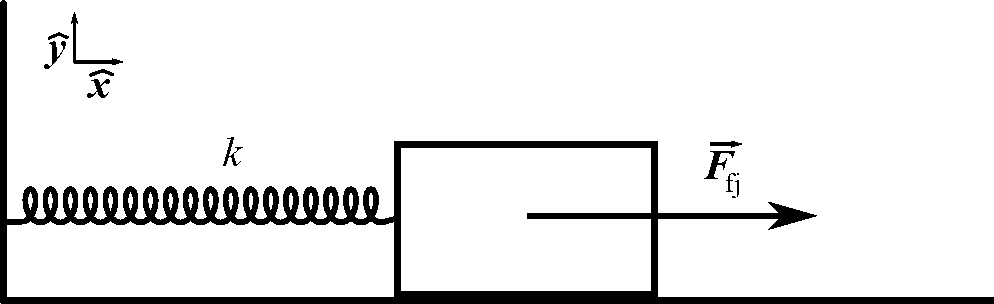
\includegraphics[width=.75\textwidth]{Analytisk-Mekanik/Fjeder.pdf}
	\caption{En klods, med massen $m$, fastspændt på en fjeder, med fjederkonstant $k$, hvor det hele er på en friktionsløs overflade. På tegningen er fjederen sammenpresset, hvorfor fjederen påvirker klodsen med en kraft, $\v{F}_\mathrm{fj}$, i den viste retning. Enhedsvektorerne i venstre hjørne viser at $x$-aksen er vandret, og $y$-aksen er lodret.} \label{fig:fjeder}
\end{figure*}
%
På figur \ref{fig:fjeder} ses en illustration af en fjeder fastspændt på en klods, hvor overfladen som klodsen bevæger sig på er friktionsløs. Fjederen har fjederkonstanten $k$ og klodsen har massen $m$. Her ses bort fra alle former for friktion, hvilket betyder at fjederkraften er den eneste kraft, der virker på klodsen. Inden dette problem løses, er det værd at overveje, hvilken løsning der forventes at få. Når fjederen er presset sammen, vil den forsøge at udvide sig, og når den er udstrakt, vil den forsøge at trække sig sammen. Det betyder, at klodsen svinger frem og tilbage omkring et ligevægtspunkt. Det forventes også, at udsvinget har en maksimal værdi samt at bevægelsen er periodisk, det vil sige at bevægelsen gentager sig. Her defineres koordinatsystemet således at klodsen i sin hvileposition er i $x = 0$, hvorved klodsens bevægelse kan beskrives med en sinus- eller cosinusfunktion, og her vælges cosinus\footnote{Havde man valgt sinus, ville det bare ændre værdien af $\delta$ med $\pi/2$. Pr. konvention vælges ofte cosinus, hvorfor det samme gøres her.} på formen
%
\begin{align} \label{eq:FjederSted}
	x(t) = A\cos(\omega t + \delta) \: ,
\end{align}
%
hvor $t$ er tiden, og $A$, $\omega$ og $\delta$ er konstanter. Cosinusfunktionen svinger mellem $-1$ og $1$, hvorfor $A$ er den maksimale afstand fra $x=0$, som klodsen kan have. $\omega$ er vinkelfrekvensen, og den hænger sammen med, hvor hurtigt klodsen svinger frem og tilbage. Fjederkonstanten $k$ er et udtryk for, hvor "hård"\;fjederen er, eller hvor meget energi det kræver, at presse fjederen sammen, mens massen $m$ er et mål for, hvor meget der skal til, for at ændre klodsens bevægelse. En logisk forventning ville derfor være, hvis $\omega$ på en eller anden måde afhænger af $k/m$. $\delta$ er en faseforskydningskonstant, og dens betydning ses ved at kigge på funktionen til tiden $t=0$. Her bliver $x(0) = A\cos\delta$, hvorfor $\delta$ er et udtryk for, hvor lodet er til tiden $t=0$. Cosinus er en periodisk funktion, der svinger frem og tilbage, hvorfor det giver mening at kunne beskrive klodsen på den måde. \\

At ligning \eqref{eq:FjederSted} faktisk beskriver klodsen, vil vi nu vise. Klodsen vil opleve en fjederkraft, $F_\mathrm{fj} = -kx$, som afhænger af fjederens forskydning fra dens ligevægtspunkt, hvilket kaldes  opførsel efter Robert Hooke. Det at fjederkraften har den form, er der ingen dybere teoretisk grund for, men det skyldes at eksperimenter viser, at fjedre kan beskrives på den måde, hvis de ikke deformeres.\footnote{Fjederkraften stiger jo mere der trækkes eller skubbes til fjederen, men trækker man for meget i fjereden, strækkes den så meget, at den holder op med at opføre sig som en fjeder. Her ses kun på tilfældet hvor $x$ ikke bliver så stor at fjederen ødelægges.} Det er antaget, at fjederkraften er den eneste i systemet, hvorfor Newtons 2. lov i 1 dimension giver, at $-kx = ma$, hvor $m$ er klodsens masse. Accelerationen $a$ er netop positionen af klodsen differentieret 2 gange med hensyn til tiden, $a = \dif[2]{t}{x}$ (differentieres et koordinat mht. tiden benyttes priknotationen, $\dif{t}{x} = \dt{x}$ og for dobbeltafledt $\ddt{x}$, fremover). Dette betyder, at vi faktisk har en 2. ordens differentialligning, der relaterer variablen $x$ til dens dobbeltafledte $\ddt{x}$
%
\begin{align} \label{eq:FjederDiffLign}
	m\ddt{x} = -kx.
\end{align}
%
Det særlige ved Newtons 2. lov er, at den giver os mulighed for, på en let og simpel måde, at opskrive de bevægelsesligninger (differentialligninger), som vi skal løse, for at kunne beskrive vores system. En beskrivelse af differentialligninger, kan findes i matematikafsnittet i appendiksetet, afsnit \ref{sec:difflign}. I modsætningen til almindelige ligninger, hvis løsninger er tal, så er løsningen til differentialligninger funktioner, og det er i matematikafsnittet bliver det forklaret, at differentialligninger kan være komplicerede at løse. Det er dog en hel del simplere at vise, at en funktion er en løsning til en differentialligning, end at finde en generel løsningsform dertil. At et tal er en løsning til en almindelige ligning, kan eftervises ved at sætte tallet ind på den ubekendtes plads, og så eftervise at ligningen går op. Det samme kan gøres med differentialligninger, hvor det så er funktionen, der indsættes. Det blev påstået at ligning \eqref{eq:FjederSted} beskriver klodsen, og derfor prøver vi nu at indsætte det i differentialligningen, ligning \eqref{eq:FjederDiffLign}. For at gøre det skal den dobbelt tidsafledte bestemmes
%
\begin{equation}
\begin{aligned}
	\ddt{x} &=\dif[2]{t}{}\left(A\cos(\omega t +\delta) \right) \\
	&= \dif{t}{}\left( -\omega A \sin(\omega t + \delta) \right) \\
	&= -\omega ^2 A \cos(\omega t + \delta ) \\
	&= -\omega^2x \: ,
\end{aligned}
\end{equation}
%
og indsættes det i ligning \eqref{eq:FjederDiffLign} fås
%
\begin{align}
	m(-\omega^2x) &= -kx \nonumber\\
	\implies \omega^2 &= \frac{k}{m} \: .
\end{align}
%
Her ses det at ligning \eqref{eq:FjederSted} opfylder ligning \eqref{eq:FjederDiffLign}, hvis $\omega^2 = k/m$. Med et snakkeargument fandt vi frem til, at $\omega$ måtte afhænge af $k/m$, og den præcise afhængighed er her opnået. Dette illustrerer at alt information, om hvordan et system opfører sig, er indeholdt i de differentialligninger, der kan opskrives ud fra Newtons love. Det kræver bare lige at de kan løses, hvilket eksempelvis kan gøres som her, ved at have et kvalificeret bud og så prøve efter, om det rent faktisk er en løsning. Man kan i nogle tilfælde bruge integration til at løse differentialligninger, hvilket kaldes separation af de variable. Ellers må man slå løsninger op eller finde numeriske løsninger med en computer.\footnote{Numeriske løsninger findes ved at sætte en computer til at regne en masse punkter, ud fra differentialligningen, til at forudsige opførslen af et bestemt system. Dette gøres tit, hvis der ikke kan laves fornuftige approksimationer til et system, eller for at teste fornuftigheden af de approksimationer man har lavet.} \\

%I vores nuværende problem med det skrå kast tager vi dog kun højde for én kraft, nemlig tyngdekraften, som i vores tilfælde er konstant $F_g = m\cdot g$, og altid rettet nedad mod jorden (dvs. i -y retningen). Da vi arbejder i to dimensioner giver dette os to rigtig simple differentialligninger, når vi anvender Newtons 2. lov:
%\begin{align}
%	F_{x,res} &= 0 = m\cdot \ddt{x} \\
%	F_{y,res} &= -m\cdot g = m\cdot \ddt{y}.
%\end{align}
%Dvs. at for det første ved vi ved reduktion af den første ligning, at $a_x = \ddt{x} = 0$, og for det andet ved vi, at $a_y = \ddt{y} = -g$. Altså at accelerationen i y-retningen er konstant -g, og at accelerationen i x-retningen er konstant 0. \\
%Nu har vi så vores to differentialligninger: hvad så? Hvordan løser vi dem så? \\
%Nu har vi jo allerede en ide om, hvordan vores bevægelse skal se ud, så lad os prøve med de tidligere nævnte udtryk for $x(t)$ og $y(t)$. \\

%Hvis $y(t) = v_{0,y} \cdot t - \frac{1}{2} \cdot g \cdot t^2$ differentieres 1 gang med hensyn til tiden får vi $v_y(t) = \dt{y} = v_{0,y} - g\cdot t$. Hvis vi gør det en gang til får vi $a_y(t) = \ddt{y} = -g$ netop som vores differentialligning giver os. Hvis vi gør det samme med $x(t) = v_{0,x}\cdot t$ får vi først $v_x(t) = \dt{x} = v_{0,x}$ og dernæst $a_x(t) = \ddt{x} = 0$, også i overensstemmelse med vores differentialligning. \\
%Derved er vi altså sikre på, at vi godt kan beskrive vores skrå kast ud fra de allerede kendte relationer for $x$ og $y$. \\ 
%
Det kan måske virke lidt som spildt arbejde at benytte differentialligningerne, hvis man kan gætte sig til en funktion, der beskriver systemet. Det svarer lidt til, at det i nogle tilfælde er ganske praktisk, at kunne gætte sig til en løsning til en almindelig ligning, men den metode afhænger af, at man har et godt gæt. Derfor er det smart at have en metode til faktisk at løse problemet, uden at skulle gætte sig frem. \\

Det skal vise sig fremadrettet at være en rigtig smart og sikker fremgangsmåde først og fremmest at finde differentialligningerne (eller nærmere bevægelsesligningerne) for ens system, hvis man ikke kender bevægelsesligningerne på forhånd. For hvis man kan finde bevægelsesligningerne, så er det eneste man mangler, nemlig at løse differentialligningen, hvor man ofte kan lave nogle simplificerende antagelser, hvis løsningen ikke er oplagt.

\section{Koordinater generelt}
I matematikafsnittet med polære koordinater, afsnit \ref{sec:PolKoord}, blev et relevant eksempel på et anderledes koordinatsystem end de kartesiske koordinater ($x,y,z$ koordinater) gennemgået, som kan være en fordel at benytte til at beskrive sit system. Indenfor mekanik er det netop denne tilgang, man har til koordinatsystemer. Man benytter dem som et redskab, til at beskrive sit system bedst og lettest muligt. Der er ikke en dybere fortolkning af ens valg af koordinater. \\

For eksempel kan et to-dimensionelt system beskrives med to rumlige, kartesiske, koordinater, $x$ og $y$. Hvis det vurderes fordelagtigt, i stedet at beskrive systemet med tre eller flere koordinater, så er man velkommen og indenfor al ret til at gøre dette. Dog mindskes kompleksiteten af et problem oftest ved at begrænse mængden af koordinater anvendt til den mindst nødvendige mængde. Ethvert almindeligt klassisk problem kan altid beskrives ud fra tre rumlige dimensioner per objekt/legeme i systemet. 
Generelt er et valgt koordinatsystem udtryk for, hvor mange dimensioner det forventes, at der skal bruges for nøjagtigt at beskrive problemet. Dette hænger tit sammen med, hvor mange retninger det forventes at et legeme kan bevæge sig i, totalt uafhængigt af andre retninger. Eksempelvis kan to uafhængige variable $a$ og $b$, samt en variabel $f(a,b)$ betragtes. At $a$ og $b$ er uafhængige af hinanden betyder her, at hvis værdien af $a$ ændres, så ændres værdien af $b$ ikke, og omvendt. Modsat er $f(a,b)$ afhængig af både $a$ og $b$, og kan derved ikke kaldes en uafhængig variabel. Ofte støder man på variable, der er implicit afhængige, hvilket betyder at man ikke skriver (eksplicit) at variablen afhænger af en anden. Dette ses tit med koordinater, hvor man ofte skriver eksempelvis $x$ i stedet for $x(t)$, idet man antager det for kendt, at $x$ afhænger af $t$. Dette er vigtigt, da man ønsker at beskrive systemet med så få uafhængige koordinater som muligt. \\ % Dette er uklart i forhold til tidsafhængighed og frie variable. Der skelnes ikke her mellem frie variable som t, og de variable vi finder udtryk for til at beskrive vores system (som afhænger af enten t eller en anden tidsafhængig variabel).
%

At koordinatsystemet her betragtes som givende udtryk for det \textit{forventede} antal uafhængige bevægelser, forklares ud fra, at det ikke altid kan vides på forhånd, hvorvidt en variabel er afhængig af andre variable eller ej. Dette finder man ud af, når man analyserer systemet, som man har med at gøre, hvorefter man kan tilrette sine koordinater efter det. Som eksempel på dette tages et simpelt pendul, som vi vil analysere senere. Umiddelbart kan pendulets bevægelse beskrives ud fra to kartesiske koordinater, $x$ og $y$, der varierer i tiden $t$, eller alternativt med to polære koordinater, med en vinkel $\phi$ og en pendullængde $r$, der også begge varierer med tiden. I dette tilfælde viser det sig dog, at længden $r$ er konstant og ikke variabel, hvormed systemet burde kunne beskrives udelukkende ud fra et udtryk for vinklen $\phi$ til tiden $t$. Men hvad med de to kartesiske koordinater $x$ og $y$? Her kan det senere vises, at den ene af de to koordinater er overflødige, da der kan findes et funktionsudtryk, som beskriver pendulets bevægelse i den ene retning ud fra dens bevægelse i den anden. Dette er dog ikke altid tilfældet, hvormed det giver god mening, at starte ud med begge koordinater. Herefter kan man altid fjerne koordinater, der ikke er nødvendige, ved ændre på sit koordinatsystem. \\

Som det vil blive nævnt senere i afsnittet om generaliserede koordinater, så er det smart at vælge sine koordinater, efter at man har gjort sig nogle indledende overvejelser omkring sit system, for at begrænse den opfattede kompleksitet af ens system. Tit vil ens system nemlig have symmetrier eller lignende restriktioner i sin bevægelse, som så vil sætte begrænsninger på antallet af koordinater (senere nævnt som frihedsgrader), der er nødvendige for at beskrive systemet. Dette bliver anvendt til, at løse de fleste af problemerne I bliver præsenteret for i dette kapitel, samt i de andre kapitler, specielt kapitlet om planetbevægelse. Udover at nævne pendulet som eksempel igen, er det dog værd at nævne, at mange systemer, med to legemer, har disse begrænsninger, og flere endda kan reduceres til kun at have en variabel (i stedet for to til hvert legeme), hvormed hele systemets bevægelse kan beskrives ved bare at kende en enkelt værdi.

\section{Roterende legemer}
Legemers bevægelse kan, i den Newtonske mekanik, deles op i to kategorier - translatorisk og rotationel bevægelse. Her menes bevægelse med og uden rotation. Vi starter med at se på den rotationelle del af legemers bevægelse, hvor der vil fokuseres på stive legemer, hvilket vil sige faste objekter, der ikke kan bøje eller deformeres. Beskrivelsen af legemers bevægelse deles op i tre dele - kinematik, energi og dynamik. Kinematik er beskrivelsen af legemers bevægelse, når bevægelsens oprindelse ikke tages med i betragtning. Dynamik beskriver hvorfor ting bevæger sig som de gør, og hvordan kinematiske bevægelser opstår. Det viser sig at energi er en vigtig størrelse at undersøge, når man skal beskrive bevægelse, hvorfor vi vil kigge på energien i både translatorisk og rotationel bevægelse.

\subsection{Kinematik}
I den translatoriske bevægelse beskrives et legemes position med en stedvektor $\v{r}$, der kan udtrykkes i forskellige koordinatsystemer. I det kartesiske koordinatsystem ser vektoren ud på en af følgende måder
%
\begin{align*}
	\v{r} = \xyz{x}{y}{z} = x\xhat + y\yhat + z\zhat \: ,
\end{align*}
%
hvilket betyder at legemet befinder sig i punktet $(x,y,z)$. Ud fra stedvektoren defineres hastighed $\v{v}$ og acceleration $\v{a}$ som\footnote{Man kan selvfølgelig differentiere stedvektoren ligeså mange gange man lyster, og selvom højere afledede bruges meget sjældent, har de faktisk nogle navne (på engelsk), som man kan underholde sig selv ved at google. Den tredjeafledede $\d^3\v{r}/\d t^3$ er dog værd at fremhæve, da den på engelsk hedder "jerk".}
\begin{equation}
    \v{v} \equiv \dt{\v{r}} \: , \qquad \v{a} \equiv \ddt{\v{r}}.
\end{equation}
%
\begin{figure}[h!]
\centering
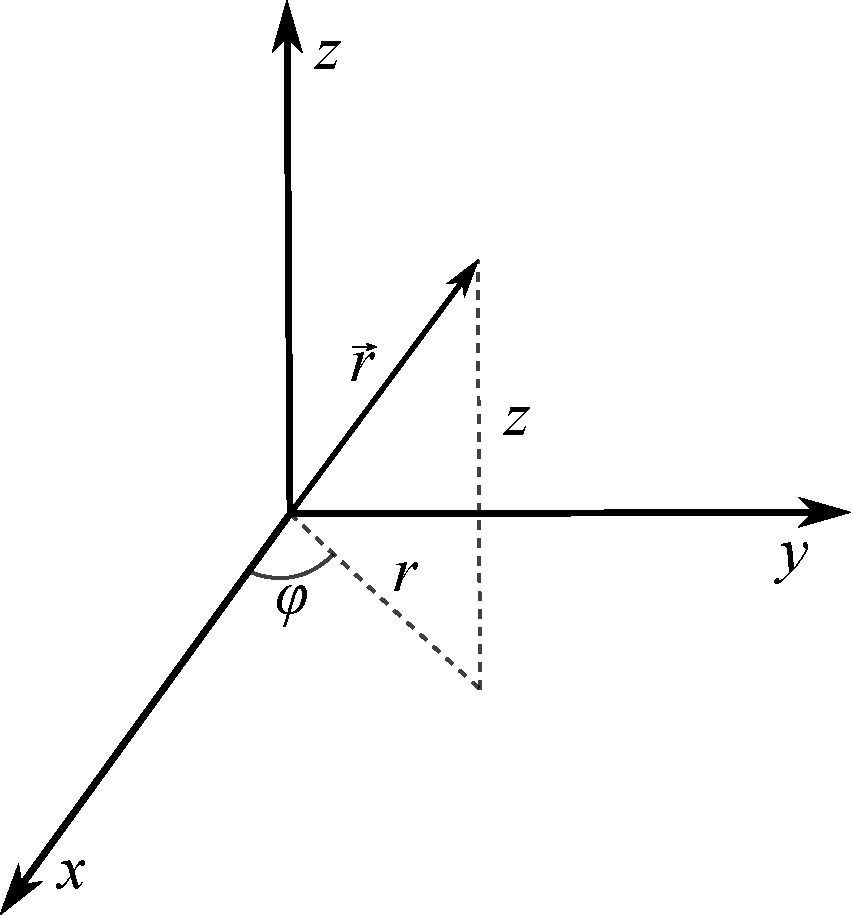
\includegraphics[width=.4\textwidth]{Analytisk-Mekanik/CylindriskeKoordinater}
\caption{I det cylindriske koordinatsystem angives afstanden til $z$-aksen som første koordinat, samt forskydningen langs samme akse som $z$-koordinat. Derudover angives vinklen med polæraksen, her ækvivalent med $x$-aksen. $z$-koordinatet er derved det samme i det kartesiske og cylindriske koordinatsystem.}
\label{fig:CylindriskeKoordinater}
\end{figure}
%
%
\subsubsection{Cylindrisk polære koordinater}
Til beskrivelsen af roterende legemer benyttes ofte cylindriske koordinater i stedet for kartesiske koordinater. Cylindriske koordinater er en tredimensionel udvidelse af de todimensionelle polære koordinater, hvor 3. koordinatet, $z$, forskyder punktet parallelt med en akse, der er ortogonal (vinkelret) på den todimensionelle plan udspændt af de polære koordinater, gennem origo, (0,0,0). I polære koordinater defineres et punkt  som origo, og ud fra det en polærakse, der angiver placeringen af vinklen på $\phi = 0$ radianer. Et punkts afstand til origo, $r$, og dets vinkel med polæraksen, $\phi$, angiver så de polære koordinater. Defineres koordinatsystemet således at polæraksen og $x$-aksen i et tilsvarende kartesisk koordinatsystem er sammenfaldende, ville $\phi$ være vinklen ift. $x$-aksen i $xy$-planen og $z$ er forskydningen ift. polærplanen, se figur \ref{fig:CylindriskeKoordinater}. Det bemærkes, at det kartesiske 3. koordinat og det cylindriske 3. koordinat er ens, og at afstanden $r$ ved udvidelsen fra polære til cylindriske koordinater forbliver uændret; det vil sige at en ændring i $z$ ikke giver en ændring i $r$. Da der kun fokuseres på legemers rotation om én akse, kan $z$-aksen defineres til at være denne rotationsakse, hvorved det cylindriske 3. koordinat forbliver uændret i tid.  \\

I polære koordinater er der en meget nyttig sammenhæng mellem et legemes totale fart og den tidsafledte af vinkelkoordinatet $\dt{\phi}$. Det antages at førstekoordinatet, $r$, er konstant i tid, $\dt{r} = 0$. Derfor kan ligning \eqref{eq:kartesisk/polaer} fra matematikafsnittet\footnote{I matematikafsnittet hedder vinklen $\theta$, hvor den her hedder $\phi$. Det betyder ikke det store hvad man kalder den, men her i kapitlet bruges $\phi$, hvor denne notation bruges konsekvent.} benyttes til at opskrive de tidsafledede af de kartesiske koordinater udtrykt ved de polære koordinater
%
\begin{equation}
\begin{aligned}
	\dt{x} &= -r\sin\phi\dt{\phi} \: , \\
	\dt{y} &= r\cos\phi\dt{\phi} \: .
\end{aligned}
\end{equation}
%
Da hastighed er en vektor, $\v{v} = \dot{x} \xhat + \dot{y} \yhat$, så er den totale fart længden af hastighedsvektoren, og den kan bestemmes vha. Pythagoras sætning
%
\begin{equation} \label{eq:SmartFart}
\begin{aligned}
	v &= \sqrt{\dt{x}^2 + \dt{y}^2} \\
	&= \sqrt{(-r\sin(\phi)\dt{\phi})^2 + (r\cos(\phi)\dt{\phi})^2} \\
	&= \sqrt{r^2\dt{\phi}^2(\cos^2\phi + \sin^2\phi)} \\
	&= r\dt{\phi}\sqrt{\cos^2\phi + \sin^2\phi} \\
	&= r\dt{\phi} \: .
\end{aligned}
\end{equation}
%
Her er grundrelationen $\cos^2\phi + \sin^2\phi = 1$ benyttet, og dette resultat bliver super anvendeligt, når der skal bestemmes energier for roterende legemer, hvilket er en essentiel del af Lagrangemekanikken, som kommer senere. Differentieres ligning \eqref{eq:SmartFart} igen med hensyn til tid fås
\begin{align}
	a = r\ddt{\phi} \: .
\end{align}

\subsubsection{Vinkelhastighed og Vinkelacceleration}
%
\begin{figure}[h!]
\centering
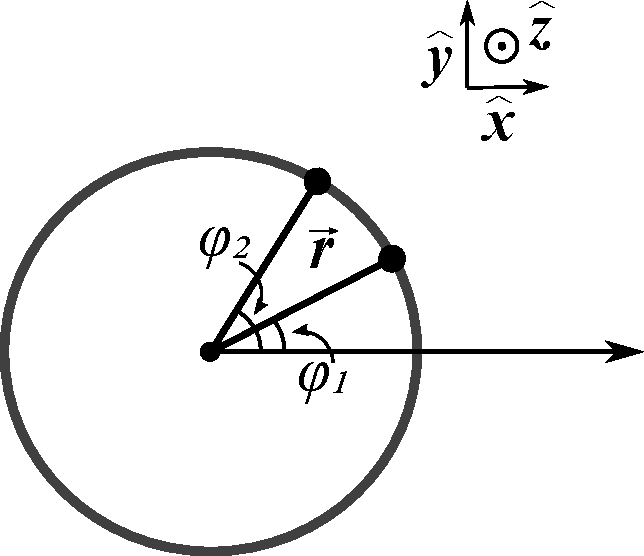
\includegraphics[width=.4\textwidth]{Analytisk-Mekanik/Roterende-Legeme}
\caption{Til to forskellige tider har det sorte punkt to forskellige vinkler med polæraksen (markeret med pil), der her er sammenfaldende med den kartesiske $x$-akse, mens legemet roterer om $z$-aksen. $\v{r}$ er en vektor fra origo til punktet, og har derfor længden $r$ og vinklen $\phi$ med polæraksen. Denne vektor ændrer sig i tid, som punktet flytter sig.}
\label{fig:Roterende-Legeme}
\end{figure}
%
Figur \ref{fig:Roterende-Legeme} viser hvordan vinklen $\phi$ ændrer sig fra tidspunktet $t_1$ til $t_2$. Helt analogt til den translatoriske bevægelse defineres vinkelhastigheden, $\omega$, og vinkelacceleration, $\alpha$, som
%
\begin{equation}
    \omega\equiv\dt{\phi} \: , \qquad \alpha\equiv\dt{\omega}=\ddt{\phi} \: .
\end{equation}
%
Vinkelhastigheden er et udtryk for, hvor hurtigt et legeme roterer og har enheden $\si{\radian/\second}$. Vinkelaccelerationen udtrykker, hvor hurtigt rotationshastigheden ændres i enheder af $\si{\radian/\second\squared}$. Her er "$\si{\radian}$"\;symbolet for enheden radianer.

\subsubsection{Inertimomentet}
Eksperimenter viser, at et legemes modstand mod acceleration ikke kun afhænger af legemets masse, men også placeringen af massen, hvorfor inertimomentet for et objekt defineres som\footnote{Symbolet $\equiv$ betyder indenfor fysik \textit{defineres som}, hvor $:=$ benyttes i matematik.}
%
\begin{equation} \label{eq:Inertimoment}
    I \equiv \sum m_ir_i^2 \: ,
\end{equation}
%
hvor $m_i$ er massen af det $i$'te masseelement og $r_i$ er samme masseelements afstand til rotationsaksen. Ethvert legeme kan tænkes som bestående af en masse små dele, kaldet masseelementer, og inertimomentet udtrykker så hvor langt fra rotationsaksen et legemes masse er placeret. Definitionen er en smule rigid, men en konceptuel forståelse er tilstrækkelig her. $I$ afhænger af den akse, som legemet  roterer om, hvilket kan forklares ved at legemer lettere kan sættes i rotation om bestemte akser end andre. Dette kan man afprøve ved at tage et objekt og prøve at rotere det på forskellige måder. Man vil mærke at nogle rotationer er lettere end andre.


\subsection{Kinetisk Energi}
For translatorisk bevægelse defineres kinetisk energi som
%
\begin{equation} \label{eq:Ktrans}
    K_{\text{trans}}=\frac{1}{2}mv_\textsc{cm}^2 \,,
\end{equation}
%
hvor $v_\textsc{cm}$ er massemidtpunktets fart. Hvis hele legemet bevæger sig med samme fart $v$ er $v_\textsc{cm} = v$, men hvis legemet eksempelvis roterer, bevæger forskellige dele af legemet sig med forskellige hastigheder. \\
Rotationskinetisk energi defineres tilsvarende som
%
\begin{equation} \label{eq:Krot}
    K_{\text{rot}}=\frac{1}{2}I\omega^2 .
\end{equation}
%
Bemærk at ligningerne \eqref{eq:Ktrans} og \eqref{eq:Krot} har præcis sammen form, idet energien i begge tilfælde er proportional med en form for inerti og en fart i anden. Den totale kinetiske energi for et roterende legeme er summen af de to ovenstående
%
\begin{equation} \label{eq:K}
    K_{\text{tot}}=K_{\text{trans}}+K_{\text{rot}} \: .
\end{equation}
%
At den totale kinetiske energi "bare"\;er summen af translatorisk og rotationel kinetisk energi, bør man strengt taget vise, men det er en smule omstændigt, hvorfor det undlades her.

\subsection{Dynamik}
%
\begin{figure}[h!]
\centering
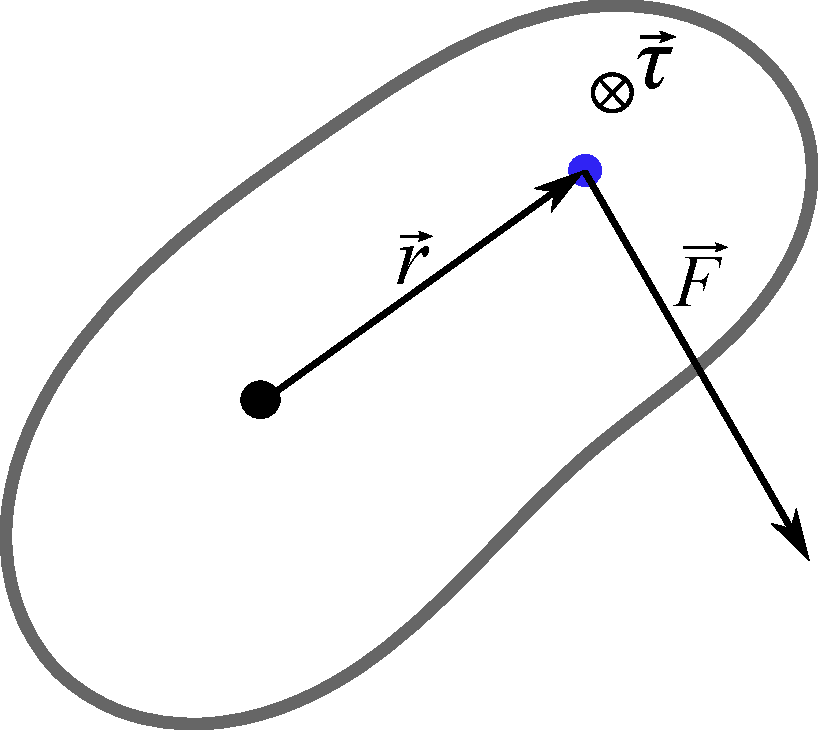
\includegraphics[width=.4\textwidth]{Analytisk-Mekanik/Kraftmoment}
\caption{En arbitrær kraft, $\v{F}$, virker i det blå punkt, hvorfor dette punkt kaldes kraftens angrebspunkt. Legemet roterer om en akse gennem det sorte punkt, der er ortogonal på tegningen. Det sorte punkt kan defineres som origo, hvorved vektoren fra rotationsaksen til kraftens angrebspunkt kaldes kraftens arm $\v{r}$. Kraftmomentet $\gv{\tau}$ peger ind i tegningen, hvilket højrehåndsreglen viser.}
\label{fig:Angrebspunkt}
\end{figure}
%
Kræfter er årsagen til bevægelse, som det kendes i fysik, og med hensyn til den translatoriske bevægelse er det ikke essentielt, hvor på legemet kraften virker, men det er det for rotationel bevægelse. Der findes mange dagligdags eksempler på dette, hvor et af de bedre er et værktøj, som en svensknøgle, der holder om en bolt. Jo længere nede på svensknøglen man holder, desto lettere er det at stramme eller løsne bolten. For at forstå fysikken bag dette, introduceres angrebspunktet for kraften $\v{F}$ som det punkt på et legeme, hvorpå kraften virker, se figur \ref{fig:Angrebspunkt}. Yderligere defineres en vektor fra rotationsaksen til kraftens angrebspunkt, hvilket kaldes kraftens arm $\v{r}$. Herved kan kraftmomentet, $\v{\tau}$, defineres
%
\begin{equation} \label{eq:Kraftmoment}
    \v{{\tau}} \equiv \v{r}\times\v{F} \: .
\end{equation}
%
Kraftmomentet er en vektor, der står ortogonalt på både kraften og dens arm, og den er parallel med rotationaksen. Kraftmomentets størrelse kan bestemmes som
%
\begin{equation} \label{eq:KraftmomentNorm}
\tau = rF\sin\theta \: ,
\end{equation}
%
hvor $\theta$ er vinklen mellem $\v{r}$ og $\v{F}$. Dette leder til Newtons 2. lov for roterende legemer
\begin{align}
	\sum\tau = I\alpha \: .
\end{align}
Det ville være super anvendeligt, hvis dette galt ligeså alment, som Newtons 2. lov, $\sum\v{F} = m\v{a}$, men det er desværre ikke tilfældet. Den gælder for legemer, der er symmetriske omkring rotationsaksen og kun for størrelsen af vektorerne.


%\begin{figure}[h!]
%\centering
%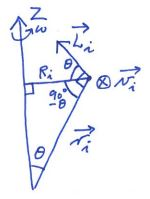
\includegraphics[width=.25\textwidth]{Analytisk-Mekanik/Impulsmoment}
%\caption{ Det $i$'te delelement af et arbitrær stift legeme, med hastighed og impulsmoment som vist, hvor kraftens arm er defineret ud fra et punkt på rotationsaksen.}
%\label{fig:Impulsmoment}
%\end{figure}

\subsubsection{Impulsmoment}
Impulsmomentet defineres ud fra den lineære impuls $\v{p}=m\v{v}$ som
%
\begin{equation} \label{eq:L}
    \v{\ell} \equiv \v{r}\times\v{p} \: .
\end{equation}
%
Størrelsen på impulsmomentet er
%
\begin{equation}
	\ell = rp\sin\theta \: ,
\end{equation}
%
hvor $\theta$ er vinklen mellem $\v{r}$ og $\v{p}$. Differentieres ligning \eqref{eq:L} med hensyn til tiden fås
\begin{equation}
    \dt{\v{\ell}} = \dif{t}{}\left(\v{r}\times\v{p}\right) = \dif{t}{\v{r}}\times m\v{v}+\v{r}\times m\dif{t}{\v{v}} = \v{v}\times m\v{v}+\v{r}\times m\v{a} = \v{r}\times\sum\v{F} = \sum\gv{\tau} \: ,
\end{equation}
idet et krydsprodukt af to parallelle vektorer er nul. Det er da vist at
\begin{equation} \label{eq:sum_tau_lig_aflede_impulsmoment}
    \sum\gv{\tau} = \dt{\v{\ell}} \: .
\end{equation}
Det kan vises at summen af de indre kraftmomenter er nul, og impulsmomentet er da bevaret, hvis og kun hvis summen af de ydre kraftmomenter er nul.

\subsection{Newtonsk beskrivelse af et pendul} \label{sec: Beskrivelse af pendul - Newton}

\begin{figure}[t]
\centering
\begin{subfigure}{.45\textwidth}
  \centering
  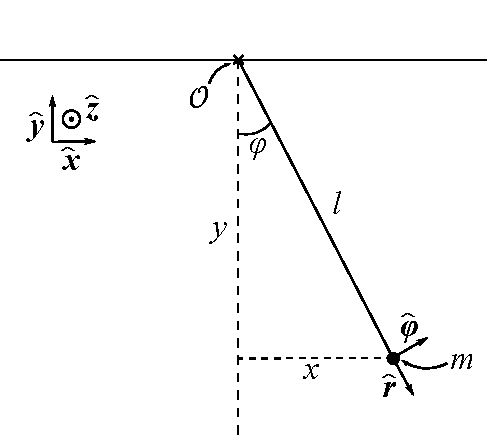
\includegraphics[width=\linewidth]{Analytisk-Mekanik/Pendul.pdf}
\caption{Skitsering af pendul med massen $m$ og længden $l$. Enhedsvektorerne til et kartesisk og cylindrisk polært koordinatsystem er indtegnet.}
\label{fig:Pendul}
\end{subfigure}
\hspace{5mm}
\begin{subfigure}{.45\textwidth}
  \centering
  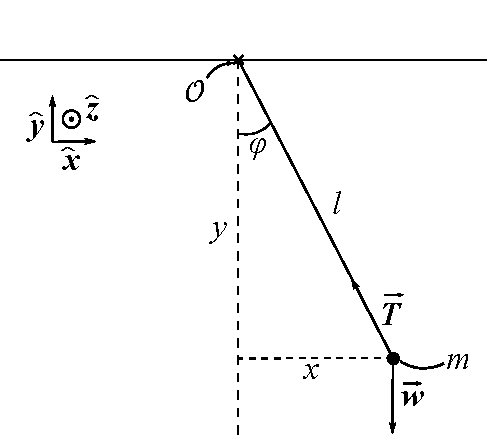
\includegraphics[width=\linewidth]{Analytisk-Mekanik/PendulKraft.pdf}
  \caption{Kraftanalyse af de på pendulloddet virkende kræfter, der alle antages at have angrebspunkt i massemidtpunktet.}
  \label{fig:Kraftanalyse}
\end{subfigure}
\caption{Tegning af pendulet, der blandt andet viser de valgte koordinatsystemer og de virkende kræfter.}
\end{figure}

I første omgang defineres et smart koordinatsystem til at beskrive pendulet. Som origo vælges pendulets ophængningspunkt, se figur \ref{fig:Pendul}. Pendulloddets position, til tiden $t$, beskrives ved en retningsvektor i cylindrisk polære koordinater $\v{r}(r,\phi,z,t)$, hvor $r$ er lodets afstand til aksen gennem origo, $\phi$ er polærvinklen, og $z$ er forskydningen fra polærplanen. Det antages at pendulet bevæger sig i ét plan, hvilket defineres som $z=0$, hvorfor $z$ forbliver uændret når tiden går. Det antages yderligere at lodets ophængning er et stift, ubøjeligt legeme, hvorfor $r=l \enspace\forall t$ \footnote{$\forall$ er matematisk notation for \textit{for alle}.}. Pendulet kan under disse antagelser beskrives fuldstændigt ved vinklen $\phi$, hvorfor stedfunktionen, $\phi(t)$, er interessant at bestemme. Pendulet kan også beskrives ved kartetiske koordinater, hvilket er indtegnet i figur \ref{fig:Pendul}, og det har visse fordele i forhold til den intuitive forståelse af systemet, når kraftanalysen udføres. \\

\noindent
På pendulet virker tyngdekraften, $\v{w}$, og en snorkraft, $\v{T}$, se figur \ref{fig:Kraftanalyse}. Det er de eneste kræfter på pendulet, idet friktion negligeres.\footnote{Det er muligt at regne med friktion, men det komplicerer situationen en del.} Tyngdekraften virker til alle tider, $t$, i negativ $y$-retning og skrives derfor som
\begin{align}
	\v{w} = -mg\yhat \: ,
\end{align}
hvor $g$ er tyngdeaccelerationen, og $\yhat$ er en enhedsvektor i $y$-retningen. Det bemærkes at $\yhat$ er en kartesisk enhedsvektor.\footnote{Teknisk set er $\yhat$ en enhedsvektor i begge koordinatsystemer, idet en enhedsvektor er en vilkårlig vektor med længden 1. Det vigtige er her at det er en enhedsvektor i den kartesiske basis og ikke i den polære.} \\
Defineres $\boldsymbol{\hat{r}}$ som en enhedsvektor parallelt med pendulets retningsvektor, hvilket også er en enhedsvektor i det polære koordinatsystem, kan snorkraften beskrives som
\begin{align}
	\v{T} = -T\boldsymbol{\hat{r}} \: ,
\end{align}
hvor $T$ er størrelsen på snorkraften, som vist på tegningen. Dette betyder, at hver kraft er simplest at beskrive i to forskellige koordinatsystemer, og faktoren $T$ har lige præcis den værdi, som får systemet til at passe. Dette viser en af svaghederne ved den Newtonske beskrivelse af mekanik - håndteringen af "tvangskræfter", eller "constraint forces" på engelsk, er kluntet. \\

\noindent
Pendulet roterer omkring ophængningspunktet, og har ved denne rotation inertimomentet $I$. Alle kræfter antages at virke på loddets massemidtpunkt, hvorfor alle kræfters arm kan beskrives som
%
\begin{align}
	\v{r} = l\boldsymbol{\hat{r}} \: ,
\end{align}
%
hvilket også er pendulloddets stedvektor. Nu kan kraftmomentet for alle de virkende kræfter bestemmes
%
\begin{equation}
\begin{aligned}
	\gv{\tau}_w &= \v{r} \times \v{w} = -mg \cdot \boldsymbol{r} \times \yhat = -mgl\sin\phi\zhat \: , \\
	\gv{\tau}_T &= \v{r} \times \v{T} = -Tl \cdot \v{r} \times \v{r} = \v{0} \: ,
\end{aligned}
\end{equation}
%
hvor subscriptet indikerer, hvilken kraft der behandles. Det samlede kraftmoment bliver derved
%
\begin{align}
	\sum\gv{\tau} = - mgl\sin\phi \zhat \: .
\end{align}
%
Antages pendulets udsvingsvinkel at være lille, kan en andenordens Taylorudvikling benyttes
%
\begin{align}
	\sin\phi\approx\phi \implies \sum\tau \approx -mgl\phi \: ,
\end{align}
%
hvor Newtons anden lov for rotationel bevægelse giver differentialligningen
%
\begin{align}
	\ddt{\phi} = \frac{1}{I}\sum\tau = -\frac{mgl}{I}\phi \: .
\end{align}
%
Denne differentialligning har løsningen
%
\begin{align} \label{eq:PendulFuld}
	\phi(t) = A\cos\left(\omega t + \delta\right), \quad \omega^2 = \frac{mgl}{I} \: ,
\end{align}
%
hvor $A$ og $\delta$ er konstanter, der er bestemt af startbetingelserne. Eftersom cosinusfunktioner giver værdier mellem $-1$ og $1$, så er $A$ den maksimalen udsvingsvinkel og $\delta$ er en faseforskydning, så pendulet kan være et hvilket som helst sted i sit udsving til tiden $t=0$.
Dette medfører, at pendulets periode bliver
%
\begin{align}
	T = \frac{2\pi}{\omega} = 2\pi\sqrt{\frac{mgl}{I}} \: .
\end{align}
%
Slutteligt kan pendulets $x$-koordinat beskrives som
%
\begin{align}
	x(t) = l\sin\phi(t) \approx l\phi(t) \: ,
\end{align}
%
hvor der til sidst igen gøres brug af en andenordens Taylorudvikling. Denne beskrivelse af et pendul kaldes et \textit{fysisk pendul}.

\subsubsection*{Matematisk pendul}
Antages pendulets masse at befinde sig i pendulets massemidtpunkt kan inertimomentet sættes til $I=ml^2$ i ligningerne fra det fysiske pendul:
%
\begin{align} \label{eq:PendulLigning}
	\ddt{\phi} = -\frac{g}{l}\phi \: ,
\end{align}
%
hvorved løsningen bliver
%
\begin{align}
	\phi(t) = A\cos\left(\omega t + \delta\right), \quad \omega^2 = \frac{g}{l} \: ,
\end{align}
%
hvilket giver en periode på
%
\begin{align}
	T = \frac{2\pi}{\omega} = 2\pi\sqrt{\frac{l}{g}} \: .
\end{align}
%
Ligning \eqref{eq:PendulLigning} er pendulligningen og rigtig mange ting i fysik kan approksimeres til en harmonisk oscillator, dvs. beskrevet ved en bevægelsesligning, for et koordinat $q$, på formen
%
\begin{align}
	\ddt{q} = -\omega^2q \: ,
\end{align}
%
hvorfor denne ligning er værd at huske på. Loddet på en fjeder var et andet eksempel på en harmonisk oscillator.

\section{Generaliserede koordinater}
I eksemplet med pendulet fremgik det, at koordinaterne $r$ og $z$ var overflødige. De var konstante i tid ved valg af et smart koordinatsystem og hele pendulet kunne beskrives ved ét koordinat, $\phi$. Dette er en generel tankegang i analytisk mekanik, da der ikke er nogen grund til at gøre problemet sværere, end det allerede er. Man kan prøve at regne pendul-eksemplet igennem, kun ved brug af de kartesiske koordinater $x$ og $y$, og man opdager hurtigt, at det er meget besværligt. Derfor introduceres konceptet generaliserede koordinater, der defineres som det sæt koordinater, der beskriver et fysisk system med det mindst mulige antal frihedsgrader. Antallet af frihedsgrader er antallet af uafhængige parametre, som beskriver et system, hvilket for pendulet er 1. Generaliserede koordinater har symbolet $q$, samt et indeks $i$, der fortæller hvilket koordinat der er tale om. Grunden til dette er, at teorien gælder for systemer med vilkårligt mange frihedsgrader. Beskrives fire partikler, som bevæger sig i en dimension, kan partiklernes koordinat noteres som $(q_1,q_2,q_3,q_4)$ eller $(q_1,q_2,...,q_4)$. Den sidste notation er ikke så praktisk i dette eksempel, men da teorien skal kunne beskrive $n$ partikler, så bliver den pludselig smart, idet koordinaterne bliver
%
\begin{align}
	(q_1,q_2,...,q_n) \: .
\end{align}
%
Ønsker man at beskrive noget som gælder for alle $n$ partikler, hvilket f.eks. kunne være at hastigheden for partiklen er givet som den tidsafledte skriver man
\begin{align}
	v_i = \dt{q}_i \: , \quad \forall \, i=1,2,...,n \: .
\end{align}
Fremover benyttes notationen $q_i$ for det $i$'te generaliserede koordinat, idet der tages højde for, at der kan være vilkårligt mange af disse, og at det også kan være nødvendigt med flere generaliserede koordinater for at beskrive én partikel. \\

Kunsten at bestemme de generaliserede koordinater bygger mange gange på at kunne genkende symmetrier. Symmetrier gør problemer lettere at håndtere, og det er derfor altid en god idé at overveje, om der er sådanne for et fysisk system. I pendul-eksemplet er der tale om cirkulær symmetri. Antagelserne at $r$ og $z$ er konstante i tid, gør at pendulets bevægelse bliver restringeret til en cirkel, hvilket kan kaldes cirkulær symmetri.

\section{Lagrangefunktion}
Generelt er Newtons love gode i sin simplicitet, med let forståelse af dem og deres anvendelse. Dette gør dem essentielle til, at have en generelt løsningsmetode til de fleste problemer. En af ulemperne ved dem er dog, at problemløsningen ofte er en slavisk proces, der kræver at man tager højde for alle kraftpåvirkninger på ens system, og kan gøre systemet mere kompliceret end det er. Et eksempel på dette er systemer, hvis bevægelse har restriktioner fra snorkræfter, normalkræfter eller lignende, der ikke udfører arbejde på systemet. Her menes der, at netop disse "constrained forces"\;sætter begrænsninger på, hvordan systemet kan bevæge sig, men at de i sig selv ikke tilføjer eller fratager energi fra systemet.Newtons love kræver dog, at de inkluderes i udregningerne for at kunne beskrive systemet korrekt. \\

Her introduceres fordelen ved Lagrangemekanikken, der tager udgangspunkt i en undersøgelse af den kinetiske og potentielle energi i et system, samt en opskrivning af differentialligninger ud fra dette, ligesom for Newtonsk mekanik (Newtons 2. lov beskriver, hvordan man opsætter differentialligninger for systemet, da $\sum\v{F} = m\v{a} = m\ddt{\v{r}}$). Ulempen ved Lagrangemekanik, i formen der introduceres her er, at den kun gælder for systemer udelukkende påvirket af konservative kræfter. Dette inkluderer derved ikke gnidningskræfter, luftmodstand og lignende.  \\

\noindent Systemet undersøges ud fra en funktion kaldet Lagrangefunktionen:
\begin{align} \label{Lagrange_funktion}
	L = K - V,
\end{align}
hvor $K$ er systemets kinetiske energi, og $V$ er systemets potentielle energi.

\subsection*{Euler-Lagrangeligningen i kartesiske koordinater}
Først vil vi beskrive vores energier ud fra kartesiske koordinater i et inertialsystem, hvilket altid kan gøres, og derefter kan det konverteres over til mere favorable, generaliserede koordinater, som vælges specifikt for hvert system. Disse gør normalt problemet lettere at løse. Vi vil desuden tage udgangspunkt i et system uden bundne kræfter (snorkraft, normalkraft), hvor vi senere kan gøre det mere generelt. \\
Den kinetiske energi er
%
\begin{align}\label{Kinetisk_kartesisk}
	K = \frac{1}{2} m v^2 = \frac{1}{2} m \dt{\v{r}}^2 = \frac{1}{2} m (\dt{x}^2 + \dt{y}^2 + \dt{z}^2) \: ,
\end{align}
%
og den potentielle energi er specifikt for systemet, men afhænger af de tre kartesiske koordinater:
%
\begin{align}\label{Potentiel_kartesisk}
	V = V(\v{r}) = V(x,y,z) \: .
\end{align}
%
Med Lagrangefunktionen opskrevet skal vi nu bruge en måde at frembringe bevægelsernes differentialligninger for systemet. Dette gøres ud fra Euler-Lagrangeligningerne:
%
\begin{equation} \label{Euler_lag_kartesisk}
\begin{aligned}
	\pdif{x}{L} &= \dif{t}{} \pdif{\dt{x}}{L} \: , \\[0.75em]
	\pdif{y}{L} &= \dif{t}{} \pdif{\dt{y}}{L} \: , \\[0.75em]
	\pdif{z}{L} &= \dif{t}{} \pdif{\dt{z}}{L} \: .
\end{aligned}
\end{equation}
%
Der fremgår altså en ligning til at udregne systemets bevægelsesligning i hver af de tre kartesiske koordinater, ud fra differentiation af Lagrangefunktionen. Det er værd at holde tungen lige i munden, når man skal udregne disse. Blandt andet skal det noteres, at der indgår to forskellige partielle differentiationer af $L$, samt en totadifferentiation med hensyn til tiden. Når der står $\partial L/\partial x$ menes der her, at man skal partielt differentiere $L$ med hensyn til $x$. Det betyder, at man skal betragte $x$ som værende den eneste variabel $L$ afhænger af, og se alle andre led som konstanter (det vil sige at eventuelle tidsafledte led $\dt{x}$ også skal ses som konstante, da der ikke eksplicit står $x$). Ydermere skal man ignorere, at $x$ også kan afhænge af tiden. Hvad så når der står $\partial L/\partial\dt{x}$? Her skal man i stedet betragte $\dt{x}$ som værende det eneste varierende led, og differentiere med hensyn til det. Derfor skal alle andre led, $x$, $y$, $z$, $\dt{y}$ og $\dt{z}$ ses som konstanter, når der differentieres. Slutteligt, så skal der totaldifferentieres med hensyn til tiden. Her skal den nye funktion $\partial L/\partial\dt{x}$ differentieres på traditionel vis med hensyn til tiden. Men det er ikke garanteret, at der eksplicit står et $t$-led nogle steder. Det skal dog huskes, at vores funktion har mulighed for at afhænge af $x,y,z,\dt{x},\dt{y},\dt{z}$, som hver især kan afhænge af tiden $t$. Derfor kan totaldifferentiationen gennemføres ved at betragte leddene $x,y,z,\dt{x},\dt{y},\dt{z}$ som funktioner, der også skal differentieres med hensyn til tiden. \\ %Kunne godt bruge et kort eksempel før vi går videre til generaliserede koordinater
%

En interessant bemærkning er faktisk, at i det ovenstående tilfælde med et system uden bundne kræfter, og ved valg af kartesiske koordinater, kan det relativt let vises at Newtons 2. lov giver præcis Euler-Lagrangeligningerne (hvilket forhåbentligt også skulle være tilfældet, da det er ækvivalente løsningsmetoder, som begge kan bruges til at komme frem til de relevante bevægelsesligninger for et system). Tag eksempelvis for $x$-koordinatet. Her fås to funktioner ved at partielt differentiere med hensyn til hhv. $x$ og $\dt{x}$:
%
\begin{align}
	\pdif{x}{L} &= \pdif{x}{}(K(\dt{x},\dt{y},\dt{z}) - V(x,y,z) ) \: , \\[0.75em]
	\pdif{\dt{x}}{L} &= \pdif{\dt{x}}{} (K(\dt{x},\dt{y},\dt{z}) - V(x,y,z) ) \: .
\end{align}
%
Her har vi, at kun $V$ afhænger eksplicit af $x$, og kun $K$ afhænger eksplicit af $\dt{x}$. Derved får vi de to resultater:
%
\begin{align}
	\pdif{x}{L} &= - \pdif{x}{V} = F_x \: , \\[0.75em]
	\pdif{\dt{x}}{L} &= \pdif{\dt{x}}{K} = \pdif{\dt{x}}{}\left(\frac{1}{2} m \left(\dt{x}^2+\dt{y}^2+\dt{z}^2\right)\right) = m\dt{x} = p_x,
\end{align}
%
hvor den totale kraft i $x$-retningen, $F_x = -\partial V/\partial x$, følger af at vi har antaget udelukkende konservative kræfter, hvorved:
%
\begin{align}
\subv{F}{res} = - \grad{V} = -\xyz{\partial V / \partial x}{\partial V / \partial y}{\partial V / \partial z} \: .
\end{align}
%Overvej om dette kan formuleres mere forståeligt, eller om det overhovedet skal med, hjælper det på forståelsen?
%
Når vi så tager Euler-Lagrangeligningen for $x$-koordinatet fåes
%
\begin{align}
	F_x = \dif{t}{p_x} = m\ddt{x},
\end{align}
%
hvilket er præcis Newtons 2. lov taget for $x$-komposanten af den resulterende kraft.

%Koordinaterne anvendt vil således være generaliserede koordinater $q_i$ $(q_1,q_2,...,q_n)$, som hver i sær udelukkende afhænger af tiden.
\subsection*{Euler-Lagrangeligningen i generaliserede koordinater}
Med den nyfundne forståelse for Lagrangefunktionen og Euler-Lagrangeligningen i kartesiske koordinater vil vi nu undersøge tilfældet, hvor vi i stedet anvender generaliserede koordinater. Fra afsnittet om generaliserede koordinater har vi, at generaliserede koordinater $(q_1,q_2,...,q_n)$ er et valgt koordinatsæt, hvor antallet af koordinater svarer til antallet af frihedsgrader for systemet. Det vil sige, at hvis vi kan nøjes med at beskrive systemet med en enkelt koordinat, som i tilfældet med det simple pendul, så har vi en generaliseret koordinat (som i dette eksempel ville være oplagt at vælge som pendulvinklen $\phi$). Her vil vi så have $n$ Euler-Lagrangeligninger, hvor $n$ er antallet af frihedsgrader for systemet, og derved antallet af generaliserede koordinater. Ud fra relationen mellem Newtons 2. lov og Euler-Lagrangeligningen for kartesiske koordinater vælges, at kalde de to relationer for henholdsvis generaliseret kraft og generaliseret impuls:
\begin{align}
	\pdif{q_i}{L} &= \text{(i'te komponent af den generaliserede kraft)} \: , \\[.5em]
	\pdif{\dt{q_i}}{L} &= \text{(i'te komponent af den generaliserede impuls)}.
\end{align}
Disse er ikke garanteret at være den fysiske kraft og impuls, som vi forstår dem, men er nærmere hvad vi ækvivalent kan forstå som dem i vores generaliserede koordinater (hvilket er grunden til navnet). Derved fås Euler-Lagrangeligningerne
%
\begin{align}\label{Euler-Lagrange}
	\pdif{q_i}{L} = \dif{t}{} \pdif{\dt{q_i}}{L}, \quad i = \{1,2,...,n\},
\end{align}
%
eller i ord:
%
\begin{align}
	\text{(generaliseret kraft)} = \text{(ændringsrate i generaliseret impuls)}.
\end{align}

\section{Eksempler på brugen af Lagrangemekanikken}
\subsection{Beskrivelse af pendul med Lagrangemekanik} \label{sec:PendulLagrange}
Igen kigges der på pendulet fra afsnit \ref{sec: Beskrivelse af pendul - Newton}, men denne gang gøres der brug af Lagrangemekanikken:

\begin{figure}[h!]
	\centering
	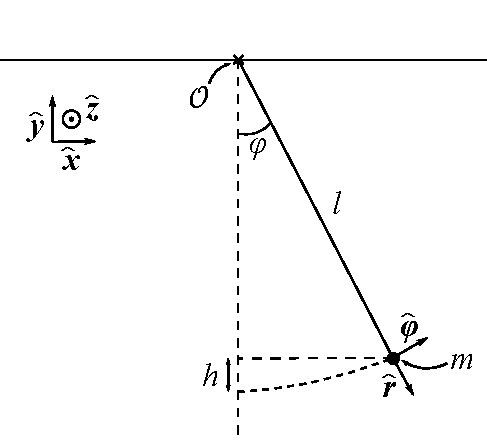
\includegraphics[width=.5\textwidth]{Analytisk-Mekanik/PendulLagrange.pdf}
	\caption{Samme pendul som i afsnit \ref{sec: Beskrivelse af pendul - Newton}. Pendulets højde, $h$, defineres ud fra nulpunktet for den potentielle energi, der vælges til at være pendulets ligevægtspunkt $(0,-l)$ (i kartesiske koordinater).}
	\label{fig:PendulLagrange}
\end{figure}

\noindent
Først kigger vi på pendulet, hvorved vi finder, at dets længde er $l$ og loddet for enden af det har masse $m$. Der defineres et nulpunkt for pendulet, hvor lodet befinder sig, når pendulet er i hvile, altså når det hænger lodret ned (se figur \ref{fig:PendulLagrange}).
Siden der kun er tale om en rotationel bevægelse, vælges et polært koordinatsystem. Den kinetiske energi af pendulet er givet ved
%
\begin{align}
	K &= \frac{1}{2} m v^2 \: ,
\end{align}
%
hvor hastigheden $v$ for en rotationel bevægelse er givet ved pendulets længde $l$ og dets vinkelhastighed $\dt{\phi}$, ligning \eqref{eq:SmartFart}, hvorfor den kinetiske energi bliver
%
\begin{align} \label{Pendul lagrange: Kinetisk energi}
	K &= \frac{1}{2} m (l \dt{\phi})^2 \: .
\end{align}
%
Den potentielle energi er givet ved
%
\begin{align}
	V &= mgh \: ,
\end{align}
%
hvor højden $h$ er givet som pendulets længde fratrukket dets projektion på $y$-aksen
%
\begin{align} \label{Pendul lagrange: Hoejde over nul}
	h &= l - l \cos(\phi) = l(1-\cos(\phi)) \: ,
\end{align}
%
hvorfor den potentielle energi bliver
%
\begin{align} \label{Pendul lagrange: Potentiel energi}
	V &= mgl \left(1-\cos(\phi) \right) \: .
\end{align}
%
I Lagrangefunktionen, ligning \eqref{Lagrange_funktion}, indsættes den kinetiske og den potentielle energi fra henholdsvis ligning \eqref{Pendul lagrange: Kinetisk energi} og ligning \eqref{Pendul lagrange: Potentiel energi}, hvilket giver følgende
%
\begin{align}
	L &= K - V = \frac{1}{2} m l^2 \phi^2 - mgl(1-\cos(\phi)) \: ,
\end{align}
%
hvorved de partielt afledede af Lagrangefunktionen med hensyn til $\phi$ og $\dt{\phi}$ bliver
%
\begin{align}
	\pdif{\phi}{L} &= - mgl \sin(\phi) \: , \label{Pendul Lagrange: Partiel afledede mht phi} \\[.5em]
	\pdif{\dt{\phi}}{L} &= m l^2 \dt{\phi} \: ,
\end{align}
%
og findes den tidsafledte af den sidste ligning fås
%
\begin{align}
	\dif{t}{} \left(\pdif{\dt{\phi}}{L}\right) &= m l^2 \ddt{\phi} \: . \label{Pendul Lagrange: Tidsafledede}
\end{align}
%
Indsættes i Euler-Lagrangeligningen, ligning \eqref{Euler-Lagrange}, den partielt aflede af Lagrangefunktionen med hensyn til $\phi$, ligning \eqref{Pendul Lagrange: Partiel afledede mht phi}, samt den tidsafledede af den partielt afledede af Lagrangefunktionen med hensyn til $\dt{\phi}$, ligning \eqref{Pendul Lagrange: Tidsafledede}, fås følgende:
%
\begin{align}
	\pdif{\phi}{L} &= \dif{t}{} \left(\pdif{\dt{\phi}}{L}\right) \nonumber \\
	\Rightarrow - mgl \sin(\phi) &= m l^2 \ddt{\phi} \: .
\end{align}
%
I ovenstående ligning isoleres vinkelaccelerationen $\ddt{\phi}$
%
\begin{align}
	\ddt{\phi} &= - \frac{g}{l} \sin(\phi) \: .
\end{align}
%
Antages det at pendulets udsving vil være små, da kan der gøres brug af Taylorudviklingen for $\sin(\phi)$, tabel \ref{Taylorseries_table}, hvorved der fås
%
\begin{align}
	\ddt{\phi} &\simeq - \frac{g}{l} \phi \: ,
\end{align}
%
hvilket er pendulligningen, ligning \eqref{eq:PendulLigning}. Hvorfor skulle dette være simplere på denne måde end den Newtonske beskrivelse? Så snart man bliver god til at differentiere rigtig, og opskrive Euler-Lagrangeligningen i nogle gode koordinater, så er denne metode markant lettere at benytte - det er bare et spørgsmål om træning.
%
\subsection{Pendul med rotationel og translatorisk bevægelse} \label{sec:elevator}
%
\begin{figure}[h!]
	\centering
	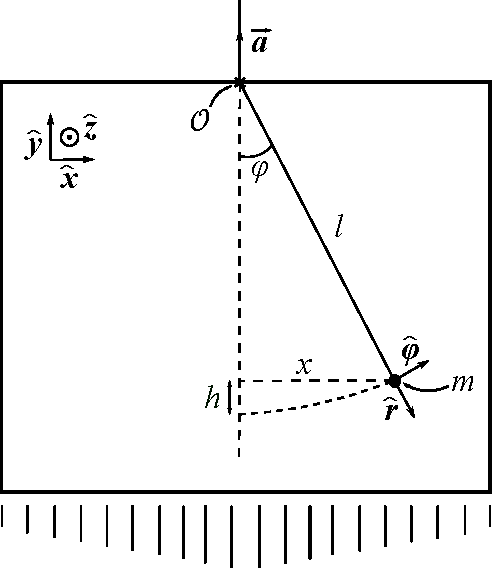
\includegraphics[scale=0.7]{Analytisk-Mekanik/PendulElevator.pdf}
	\caption{Samme pendul som i figur \ref{fig:PendulLagrange}, dog nu placeret i en lineært accelererende elevator.}
	\label{fig:PendulElevator}
\end{figure}
%
Et anden eksempel, hvor der kan gøres brug af Lagrangemekanikken er, når et problem indeholder både translatorisk og rotationel bevægelse, hvilket kan illustreres af et pendul i en elevator, figur \ref{fig:PendulElevator}. Her bevæger lodet i pendulet sig ved en rotationel bevægelse, hvorimens elevatoren bevæger sig med en translatorisk bevægelse, hvilket her er ved konstant acceleration. Først findes koordinaterne, $x$ og $y$, for loddet samt de tidsafledede af disse:
\begin{equation}
	\begin{aligned}
		x &= l \sin(\phi) \: , \\
		\dt{x} &= l \cos(\phi) \dt{\phi} \: , \\
		y &= l \big(1-\cos(\phi) \big) + \frac{1}{2} at^2 \: , \\
		\dt{y} &= l \sin(\phi) \dt{\phi} + at \: ,
	\end{aligned}
\end{equation}
hvor formlen for $y$ fremkommer som kombination af pendulets $y$-koordinat i forhold til elevatoren, ligning \eqref{Pendul lagrange: Hoejde over nul}, og elevatorens stedfunktion
\begin{align}
	y_{elevator}(t) &= \frac{1}{2}at^2 + v_{0,elevator} t + y_{0,elevator} \: ,
\end{align}
hvor $y_{0,elevator} = v_{0,elevator} = 0$ grundet vores valg af koordinatsystem. Dette valg foretages, da det gør $y$-koordinaten nemmere at regne med.

\noindent
Systemets kinetiske og potentielle energi findes herudfra som henholdsvis
%
\begin{align}
	K &= \frac{1}{2} m \left( \dt{x}^2 + \dt{y}^2 \right) \nonumber \\
	&= \frac{1}{2} m \left[ \left( l^2 \cos^2(\phi) \dt{\phi} \right) + \left( l^2 \sin^2(\phi) \dt{\phi} + a^2t^2 + 2 l \sin(\phi) \dt{\phi} a t \right) \right] \nonumber \\
	&= \frac{1}{2} m \left( l^2\phi^2 + a^2t^2 + 2l\sin(\phi)\dt{\phi}at \right) \, ,
\end{align}
%
og
%
\begin{align}
	V &= mgy = mg \left[ l \left( 1 - \cos(\phi) \right) + \frac{1}{2}at^2 \right] \: ,
\end{align}
%
hvorved Lagrangefunktionen bliver
%
\begin{align}
	L &= K-V = \frac{1}{2} m \left( l^2\dt{\phi}^2 + a^2t^2 + 2l\sin(\phi)\dt{\phi}at \right) - mg \left[ l \left( 1 - \cos(\phi) \right) + \frac{1}{2}at^2 \right] \: .
\end{align}
%
De partielt afledede af Lagrangefunktionen i forhold til henholdsvis $\phi$ og $\dt{\phi}$, samt den tidsafledede af sidste findes:
%
\begin{align}
	\pdif{\phi}{L} &= ml\cos(\phi)\dt{\phi}at - mgl\sin(\phi) \: , \\
	\pdif{\dt{\phi}}{L} &= ml^2\dt{\phi} + ml\sin(\phi)at \: , \\
	\dif{t}{} \left(\pdif{\dt{\phi}}{L}\right) &= ml^2\ddt{\phi} + ml\cos(\phi)\dt{\phi}at + ml\sin(\phi)a \: .
\end{align}
%
Indsættes dette i Euler-Lagrangeligningen fås
%
\begin{align}
	\pdif{\phi}{L} &= \dif{t}{}\left( \pdif{\dt{\phi}}{L} \right) \nonumber \\
	 \Rightarrow ml\cos(\phi)\dt{\phi}at - mgl\sin(\phi) &= ml^2\ddt{\phi} + ml\cos(\phi)\dt{\phi}at + ml\sin(\phi)a \: .
\end{align}
%
Heri isoleres vinkelaccelerationen
%
\begin{align}
	\ddt{\phi} &= - \frac{g+a}{l}\sin(\phi) \: ,
\end{align}
%
og antages pendulets udsving at være lille, kan dette Taylorudvikles til
\begin{align}
	\ddt{\phi} &\simeq - \frac{g+a}{l}\phi \: ,
\end{align}
hvilket er på samme form som pendulligningen, hvorfor dette kan ses som et stillestående system med en ændret tyngdeacceleration, $\tilde{g} = g + a$.

\subsection{Karrusel: System uden potentiel energi} \label{sec:Karrusel}
\begin{figure}
	\centering
	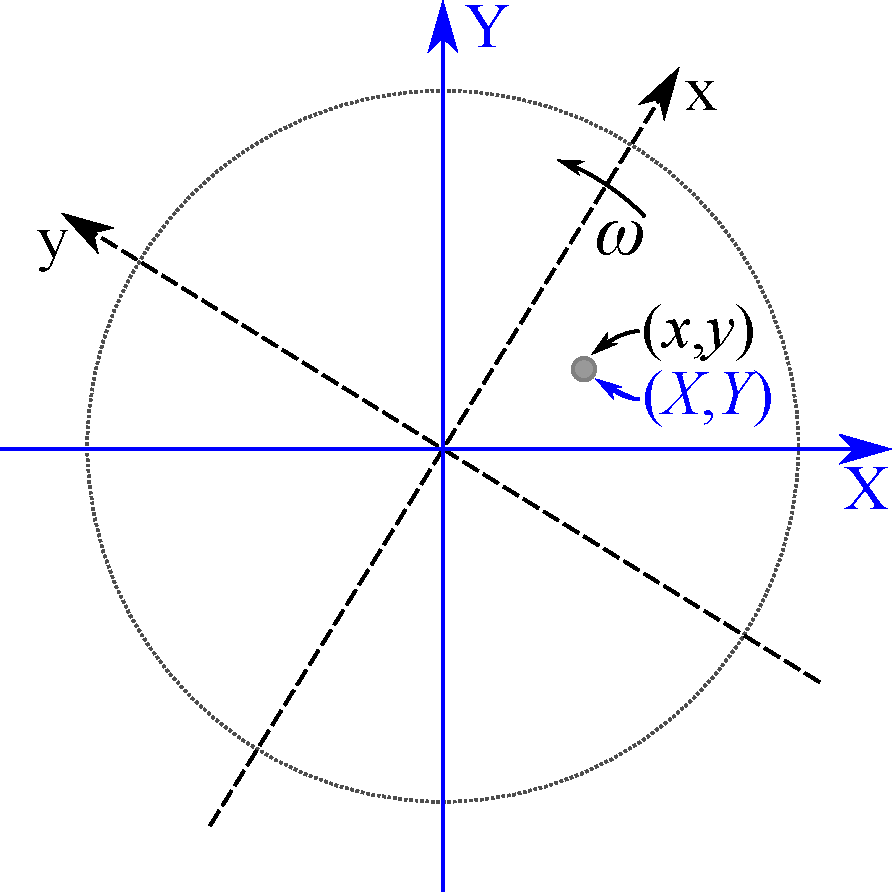
\includegraphics[width=0.4\columnwidth]{Analytisk-Mekanik/Karussel.pdf}
	\caption{Roterende karussel. Det stiplede sorte koordinatsystem roterer med karussellen således, at et punkt på karusellen i dette koordinatsystem altid har koordinaterne $(x,y)$. I det fastlåste blå koordinatsystem roterer karussellen, hvorfor førnævnte punkt i dette koordinatsystem vil have skiftende koordinater, der er givet ved $(X,Y)$, ligning \eqref{eq:Karussel_X_Y_koordinater}.}
	\label{fig:Karussel}
\end{figure}

Ovenfor har der været kigget på systemer, der har haft både kinetisk og potentiel energi, hvorfor der nu ses på et system uden potentiel energi: En karrusel, figur \ref{fig:Karussel}.

\noindent
I dette system betragtes en partikel med masse $m$, der bevæger sig relativt til et roterende koordinatsystem, som følger karrusellen (stiplet koordinatsystem i figur \ref{fig:Karussel}). I dette koordinatsystem har partiklen koordinaterne $(x,y)$. Betragtes dette system ud fra et stillestående koordinatsystem (blåt koordinatsystem i figur \ref{fig:Karussel}) med samme origo, vil karrusellen rotere med en vinkelhastighed $\omega$. I dette koordinatsystem vil partiklens koordinater være $(X,Y)$. Sammenhængen mellem partiklens koordinater i de to koordinatsystemer er givet ved\footnote{Dette fås ved at gange en rotationsmatrix på stedvektoren $\xy{x}{y}$, hvilket her bare tages for gode varer.}
%
\begin{equation} \label{eq:Karussel_X_Y_koordinater}
	\begin{aligned}
		X &= x \cos(\omega t) - y \sin(\omega t) \: , \\
		Y &= x \sin(\omega t) + y \cos(\omega t) \: .
	\end{aligned}
\end{equation}
%
For at finde den kinetiske energi, beregnes de afledede af koordinaterne, hvilket giver
%
\begin{equation}
	\begin{aligned}
		\dt{X} &= \dt{x} \cos(\omega t) - \omega x \sin(\omega t) - \dt{y} \sin(\omega t) - \omega y \cos(\omega t) \: , \\
		\dt{Y} &= \dt{x} \sin(\omega t) + \omega x \cos(\omega t) + \dt{y} \cos(\omega t) - \omega y \sin(\omega t) \: .
	\end{aligned}
\end{equation}
%
Hernæst beregnes summen af de kvadrerede $\dt{X}$- og $\dt{Y}$-koordinater:
%
\begin{align} \label{eq:KarusselHastighed}
	\dt{X}^2 + \dt{Y}^2 &= \dt{x}^2 + \omega^2 x^2 + \dt{y}^2 + \omega^2 y^2 - \dt{x}y \omega + x \dt{y} \omega + x \dt{y} \omega - \dt{x} y \omega \nonumber \\
	&= \dt{x}^2 - \dt{y}^2 + \omega(x^2 + y^2) + 2 \omega (x \dt{y} - \dt{x} y) \: .
\end{align}
%
De første fire led i ligning \eqref{eq:KarusselHastighed} fremkommer på samme måde, og her forklares blot fremkomsten af $\dt{x}^2$ leddet: Kvadreres $\dt{X}$ og $\dt{Y}$ fremkommer led som er kvadrerede, for eksempel
%
\begin{align*}
	[\dt{x} \cos(\omega t)]^2 &= \dt{x}^2 \cos^2(\omega t) \: , \\
	[\dt{x} \sin(\omega t)]^2 &= \dt{x}^2 \sin^2(\omega t) \: .
\end{align*}
%
Siden summen af de kvadredede $\dt{X}$- og $\dt{Y}$-koordinater beregnes, vil man få
\begin{align*}
	\dt{x}^2 \cos^2(\omega t) + \dt{x}^2 \sin^2(\omega t) &= \dt{x}^2 (\cos^2(\omega t) + \sin^2(\omega t)) = \dt{x}^2 \: ,
\end{align*}
%
da $\cos^2(\omega t) + \sin^2(\omega t) = 1$, hvilket kaldes grundrelationen.

\noindent
For de resterende fire led er der også gjort brug af grundrelationen, men her blot mellem krydsleddene: Tages et eksempel kan det ses at
%
\begin{align*}
	\left[\dt{x}\cos(\omega t)\right] \left[-\omega y\cos(\omega t)\right] &= -\dt{x}\omega y \cos^2(\omega t) \: , \\
	\left[\dt{x}\sin(\omega t)\right] \left[-\omega y\sin(\omega t)\right] &= -\dt{x}\omega y \sin^2(\omega t) \: .
\end{align*}
%
Sammenlægges disse to led fås
%
\begin{align*}
	-\dt{x}\omega y \cos^2(\omega t) -\dt{x}\omega y \sin^2(\omega t) &= -\dt{x}\omega y \left(\cos^2(\omega t) + \sin^2(\omega t)\right) = -\dt{x}\omega y \: .
\end{align*}

\noindent
De resterende krydsled fra sammenlægningen $\dt{X}$ og $\dt{Y}$ går ud med hinanden, eksempelvis
%
\begin{align*}
	\left[\dt{x}\cos(\omega t)\right] \left[-\omega x \sin(\omega t)\right] &= -\dt{x}x\omega\cos(\omega t)\sin(\omega t) \: , \\
	\left[\dt{x}\sin(\omega t)\right] \left[\omega x \cos(\omega t)\right] &= \dt{x}x\omega\cos(\omega t)\sin(\omega t) \: ,
\end{align*}
%
hvorfor disse ikke indgår i ligning \eqref{eq:KarusselHastighed}.

\noindent
Ud fra ligning \eqref{eq:KarusselHastighed} fås følgende kinetisk energi
%
\begin{align}
	K &= \frac{1}{2} m \left(\dt{X}^2 + \dt{Y}\right) = \frac{1}{2} m \left[ \dt{x}^2 - \dt{y}^2 + \omega(x^2 + y^2) + 2 \omega (x \dt{y} - \dt{x} y) \right] \: ,
\end{align}
%
og da der ingen potentiel energi er i systemet, bliver Lagrangefunktionen
%
\begin{align}
	L &= K = \frac{1}{2} m \left[ \dt{x}^2 - \dt{y}^2 + \omega(x^2 + y^2) + 2 \omega (x \dt{y} - \dt{x} y) \right] \: .
\end{align}
%
Fra denne Lagrangefunktion kan følgende partielt afledede med hensyn til $x$ og $\dt{x}$ findes
%
\begin{align}
	\pdif{x}{L} &= \frac{1}{2} m \left[ 2\omega^2x + 2\omega \dt{y} \right] = m \left( \omega^2x + \omega \dt{y} \right) \: , \\
	\pdif{\dt{x}}{L} &= \frac{1}{2} m \left[ 2 \dt{x} - 2\omega y \right] = m \left( \dt{x} - \omega y \right) \: , \\
	 \dif{t}{} \left( \pdif{\dt{x}}{L} \right) &= m \left( \ddt{x} - \omega \dt{y} \right) \: ,
\end{align}
%
hvorved Euler-Lagrangeligningen bliver
%
\begin{align}
	\pdif{x}{L} &= \dif{t}{} \left( \pdif{\dt{x}}{L} \right) \nonumber \\
	\Rightarrow m \left( \omega^2 x + \omega \dt{y} \right) &= m \left( \ddt{x} - \omega \dt{y} \right) \: ,
\end{align}
%
så bevægelsesligningen bliver
%
\begin{align} \label{eq:xKarusel}
	\ddt{x} &= \omega^2x + 2 \omega \dt{y} \: .
\end{align}

\noindent
For $y$ og $\dt{y}$ bliver de partielt afledede
%
\begin{align}
	\pdif{y}{L} &= \frac{1}{2} \left[ 2 \omega^2y - 2\omega\dt{x} \right] = m \left( \omega^2y - \omega \dt{x} \right) \: , \\
	\pdif{\dt{y}}{L} &= \frac{1}{2} \left[2 \dt{y} + 2 \omega x \right] = m \left( \dt{y} + \omega x \right) \: , \\
	\dif{t}{} \left(\pdif{\dt{y}}{L}\right) &= m \left( \ddt{y} - \omega \dt{x} \right) \: ,
\end{align}
%
hvorved Euler-Lagrangeligningen bliver
%
\begin{align}
	\pdif{y}{L} &= \dif{t}{} \left(\pdif{\dt{y}}{L}\right) \nonumber \\
	\Rightarrow m \left( \omega^2 y-\omega \dt x \right) &= m \left( \ddt{y} - \omega \dt{x} \right) \: ,
\end{align}
%
og der fås følgende bevægelsesligning for partiklen i $y$-retningen
%
\begin{align} \label{eq:yKarusel}
	\ddt{y} &= \omega^2y - 2 \omega \dt{x} \: .
\end{align}

\noindent
Det kan med nogle lettere bøvlede udregninger vises, at Corioliskraften og centrifugalkraften er givet som
%
\begin{equation} \label{eq:FiktiveKraefter}
\begin{aligned}
	\v{F}_\mathrm{cor} &= 2m\dt{\v{r}}\times\v{\Omega} \: , \\
	\v{F}_\mathrm{cf} &= m(\v{\Omega} \times \v{r}) \times \v{\Omega} \: ,
\end{aligned}
\end{equation}
%
hvor $\v{r}$ er stedvektoren for det legeme, som kræfterne påvirker, og $\v{\Omega}$ er vinkelhastighedsvektoren for det roterende koordinatsystem, som legemet befinder sig i. I dette eksempel roterer karrusellen med vinkelhastigheden $\omega$ omkring $z$-aksen, hvorfor $\v{\Omega} = \omega\zhat$. Enhver vektor kan i kartesiske koordinater skrives på formen $\v{r} = x\xhat + y\yhat + z\zhat$. Af denne grund kan Corioliskraften skrives som
%
\begin{equation}
\begin{aligned}
	\v{F}_\mathrm{cor} &= 2m(\dt{x}\xhat + \dt{y}\yhat + \dt{z}\zhat) \times \omega\zhat \\
	&= 2m\omega(-\dt{x}\yhat + \dt{y}\xhat) \: ,
\end{aligned}
\end{equation}
%
og tilsvarende bliver centrifugalkraften
%
\begin{equation}
\begin{aligned}
	\v{F}_\mathrm{cf} &= m[\omega\zhat \times (x\xhat + y\yhat + z\zhat)] \times \omega\zhat \\
	&= m\omega^2[x\yhat - y\xhat] \times \zhat \\
	&= m\omega^2(x\xhat + y\yhat) \: .
\end{aligned}
\end{equation}
%
Bruges Newtons 2. lov på summen af de fiktive kræfter fås
\begin{align}
	\sum\v{F} &= \v{F}_\mathrm{cor} + \v{F}_\mathrm{cf} \nonumber\\
	\Rightarrow m(\ddt{x}\xhat + \ddt{y}\yhat) &= 2m\omega(-\dt{x}\yhat + \dt{y}\xhat) + m\omega^2(x\xhat + y\yhat) \: ,
\end{align}
%
og samles $x$- og $y$-komposanterne for sig fås
%
\begin{equation}
	\begin{aligned}
		\ddt{x} &= \omega^2x + 2\omega\dt{y} \: , \\
		\ddt{y} &= \omega^2y - 2\omega\dt{x} \: .
	\end{aligned}
\end{equation}
%
Dette er præcis de samme ligninger, som ligningerne \eqref{eq:xKarusel} og \eqref{eq:yKarusel}, hvorfor ovenstående kan tænkes som en pseudoudledning af Coriolis- og centrifugalkraften, og det illustrerer også, at de er effekter, som rotationen skaber fra den kinetiske energi i systemet. Grunden til at det ikke er en rigid udledning er, at den er bundet op på det kartesiske koordinatsystem og én specifik rotation. Karrusellen illustrerer dog eksistensen af disse fiktive kræfter, til en vis grad hvor de kommer fra, og den belyser hvad disse kræfter er for nogle størrelser.


\section{Perspektiver i Analytisk Mekanik}
Euler-Lagrangeligningen giver én andenordens differentialligning for hvert generaliseret koordinat, men disse kan være svære at løse. Nogle gange er det simplere at få to koblede differentialligninger pr. generaliseret koordinat, hvilket kræver en ny formulering af mekanikken.

\subsection{Hamiltonformalismen}
Tankegangen minder meget om den fra Lagrangeformalismen, hvorfor der kan tages udgangspunkt i den til at illustre idéen. Her defineres en Hamiltonfunktion, $H$, af $n$ generaliserede koordinater ud fra Lagrangefunktionen
%
\begin{align} \label{eq:HamiltonDefinition}
	H(q_1,q_2,...,q_n,p_1,p_2,...,p_n,t) \equiv \sum_i^np_i\dt{q}_i - L \: ,
\end{align}
%
hvor $p_i$ er den generaliserede impuls svarende til det $i$'te generaliserede koordinat $q_i$. Det er vigtigt at pointere at en Hamiltonfunktion først kan kaldes en Hamiltonfunktion, når den er udtrykt udelukkende ved de generaliserede stedkoordinater og impulser. Det kommer til at give mening under udledningen af Hamiltons ligninger, der netop er udtrykt ved disse parametre. Den generaliserede impuls er defineret ud fra Lagrangefunktionen som
\begin{align} \label{eq:generaliseretImpuls}
	p_i \equiv \pdif{\dt{q}_i}{L} \: .
\end{align}
I mange tilfælde er Hamiltonfunktionen givet ud fra et systems energier
\begin{align} \label{eq:H=E}
	H = K + V = E \: ,
\end{align}
og den er faktisk ofte systemets samlede energi, hvilket dog ikke uddybes her. \\%, se opgave \ref{opg:HamiltonEnergi}. \\
Differentieres ligning \eqref{eq:HamiltonDefinition} partielt med hensyn til det $i$'te generaliserede koordinat fås
%
\begin{align}
	\pdif{q_i}{H} = p_i\pdif{q_i}{\dt{q}_i} + \pdif{q_i}{p_i}\dt{q_i} - \pdif{q_i}{L} - \pdif{\dt{q}_i}{L}\pdif{q_i}{\dt{q}_i} \: .
\end{align}
%
Alle disse differentialer kommer af at der er tale om en produktfunktion og en sammensat funktion, og man er nød til at tage højde for, at der kan være bidrag fra alle led. Ved brug af ligning \eqref{eq:generaliseretImpuls} ses det, at første og sidste led er ens, men med modsat fortegn. Derudover afhænger $p_i$ ikke eksplicit af $q_i$, hvorfor dens partielt afledte er nul. Dette skyldes at de generaliserede koordinater med tilhørende generaliserede impulser er en komplet basis for systemet, hvilket blandt andet betyder, at ingen af dem kan udtrykkes ved de andre, hvorfor deres partielt afledte med hensyn til hinanden skal være nul. \\
Ved brug af Euler-Lagrangeligningen, ligning \eqref{Euler-Lagrange}, og definitionen på generaliseret impuls, ligning \eqref{eq:generaliseretImpuls}, opnås den første af Hamiltons ligninger:
%
\begin{align}
	\pdif{q_i}{H} = -\pdif{q_i}{L} = -\el{\dt{q_i}} = -\dif{t}{p_i} = -\dt{p_i} \: .
\end{align}
%
Prøves det nu at opskrive den partielt afledede af Hamiltonfunktionen med hensyn til den generaliserede impuls fås
%
\begin{align}
	\pdif{p_i}{H} = p_i\pdif{p_i}{\dt{q}_i} + \pdif{p_i}{p_i}\dt{q_i} - \pdif{p_i}{L} - \pdif{\dt{q}_i}{L}\pdif{p_i}{\dt{q}_i} \: .
\end{align}
%
Pr. definition er Lagrangefunktionen en funktion at de generaliserede koordinater og disses afledte, hvorfor $\partial L/\partial p_i = 0$. Med henvisning til ligning \eqref{eq:generaliseretImpuls} ses det også, at første og sidste led er ens, og da den partielt afledte af en funktion med hensyn til sig selv er 1, fås det at
%
\begin{align}
	\pdif{p_i}{H} = \pdif{p_i}{p_i}\dt{q_i} =  \dt{q}_i \: .
\end{align}
%
Dette er Hamiltons 2. ligning, og skrives de to op sammen er det
%
\begin{equation}
\begin{aligned}
	\pdif{q_i}{H} &=  -\dt{p}_i \: , \\
	\pdif{p_i}{H} &=  \dt{q}_i \: .
\end{aligned}
\end{equation}
%
Her vil der ikke gås i detaljen med, hvorfor Hamiltonformalismen kan være smart sammenlignet med Lagrangeformalismen, og det virker da også umiddelbart som ekstra arbejde, at skulle omskrive Lagrangefunktionen til en gyldig Hamiltonfunktion og så indsætte i Hamiltons ligninger, når man bare kunne have indsat i Euler-Lagrangeligningen. Her må man som læser bare stole på, at der eksisterer tilfælde, hvor Hamiltonformalismen er nemmere at benytte. Et mindre flyvsk argument for at introducere Hamiltonformalismen er dog at kvantemekanikken bygger på netop dette, hvilket ses i form af Hamiltonoperatoren, og alt dette introduceres i kapitel \ref{cha:Kvant} om netop kvantemekanik.

% Herfra overlades det sidste til EHK at finde et hjem for =)

%\subsection{Fra klassisk mekanik til kvantemekanik}
%Kvantemekanikken bygger dog på Hamiltonformalismen, hvorfor idéen med dette afsnit er at introducere Hamiltonfunktionen, der omskrives til Hamiltonoperatoren, $\op{H}$, som kan betragtes som grundstenen for kvantemekanikken, fordi den tidsuafhængige eller stationære Schrödingerligning kan skrives som egenværdiproblemet
%
%\begin{align}
%	\op{H}\psi = E\psi
%\end{align}
%
%Her går $\psi$'erne ikke ud med hinanden, da dette er formuleret ved hjælp af den gren af matematikken, der hedder lineær algebra, hvilket gør matematikken meget lettere, når først man har styr på denne disciplin. Det er dog meget abstrakt at lære, hvorfor det ikke vil beskrives detaljeret her. Hamiltonoperatoren kan opskrives ud fra den klassiske Hamiltonfunktion ved at benytte at kinetisk energi kan udtrykkes på følgende måde for et generaliseret koordinat
%
%\begin{align} \label{eq:K(p)}
%	K =  \frac{p^2}{2m}
%\end{align}
%
%hvilket kan motiveres ved at den generaliserede impuls ofte kan skrives på formen $p = m\dt{q}$, som giver definitionen på kinetisk energi, ved indsættelse i ligning \eqref{eq:K(p)}. Derved giver ligning \eqref{eq:H=E} at
%
%\begin{align}
%	H = K + V = \frac{p^2}{2m} + V
%\end{align}
%
%som på operatorform er
%
%\begin{align}
%	\op{H} = \frac{\op{p}^2}{2m} + V
%\end{align}
%
%Benyttes impulsoperatoren i tabel \ref{tab:operatorer_i_kvant} nu, samt definitionen på tallet $i$, nemlig at $i^2 = -1$ fås hamiltonoperatoren fra samme tabel
%
%\begin{align}
%	\op{p}^2 &= \left(-i\hbar\pdif{x}{}\right)^2 = \hbar^2\pdif[2]{x}{} \\
%	\op{H} &= \frac{\op{p}^2}{2m} + V = -\frac{\hbar^2}{2m}\pdif[2]{x}{} + V
%\end{align}
%
%Der er hermed dannet en bro mellem klassisk mekanik og kvantemekanik, og målet med dette er at vise at en sådan bro eksisterer fremfor en rigid gennemgang af Hamiltonformalismen og dens klassiske mangfoldigheder. \\

%Konkluderende kan det siges at metoden til at analysere et kvantemekanisk system er at opskrive systemets kinetiske og potentielle energi, for derefter at opstille systemets Hamiltonfunktion. Denne omskrives til en Hamiltonoperator, som giver mening for systemet, og derefter løses den stationære Schrödingerligning. Dette kan lyde relativt simpelt, men der kan komme en del komplikationer i forbindelse med eksempelvis skridtet med at omskrive Hamiltonfunktionen til en passende Hamiltonoperator.
%\chapter{Analytisk Mekanik}
%
%
\section*{Koordinatsystemer}
\begin{opgave}{Gode koordinatsystemer}{1}
At få valgt et smart koordinatsystem er essentielt i analytisk mekanik.
\opg Beskriv hvad der kendetegner et smart valg af koordinatsystem?
\opg Hvorfor kan det smarte koordinatsystem identificeres ud fra symmetri?
\opg Hvilket koordinatsystem er smartes for et problem med: \\
a) Plansymmetri. \\
b) Cylindrisk symmetri. \\
c) Sfærisk symmetri. \\
Forklar hvorfor?
\end{opgave}
%
%
\begin{opgave}{Generaliserede koordinater}{1}
Betragt et objekt der er fanget på en ring med centrum i origo, $(0,0)$, og radius $R$.
\opg Definer et sæt polære koordinater $(r,\phi)$, og skriv de kartesiske koordinater op med disse.
\opg Hvor mange af de kartesiske koordinater ændres, når objektet bevæger sig på ringen?
\opg Hvor mange af de polære koordinater ændres, når objektet bevæger sig på ringen?
\opg Hvor mange koordinater skal der bruges for at beskrive objektets bevægelse?
\opg Hvad er det smarte koordinatvalg?
\end{opgave}
%
%
\begin{opgave}{Brint}{2}
Hydrogenisotopen $^1$H består af en proton med massen $m_p$ og ladningen $e$ (elementarladningen), samt en elektron med massen $m_e$ og ladningen $-e$. Fra elektrostatik\footnote{Elektrostatik er studiet af elektriske felter dannet af stillestående (statiske) elektriske ladninger.} oplyses det, at kraften fra en punktladning $Q_1$ med stedvektor $\v{r}_1$ på en punktladning $Q_2$ med stedvektor $\v{r}_2$ er
\begin{align} \label{eq:F_el}
	\v{F} = \frac{Q_1Q_2}{4\pi\epsilon_0}\frac{\v{r}_2-\v{r}_1}{|\v{r}_2-\v{r}_1|^3} \: ,
\end{align}
hvor $\epsilon_0$ er en konstant, der kaldes vakuumpermittiviteten. Punktladninger er ladninger uden udstrækning, hvorfor de eksisterer i ét punkt i rummet og kun det punkt. Elektroner og protoner er så små, at de kan beskrives som punktladninger, hvorfor ligning \eqref{eq:F_el} kan benyttes.
\opg Skitser situationen og indtegn systemets massemidtpunkt. Hint: Se formel (\ref{CM}) for definitionen af massemidtpunktet (på engelsk center of mass, forkortes CM).
\opg Hvad betyder $|\v{r}_2-\v{r}_1|$ fysisk?
\opg Indtegn kræfterne på begge ladninger i jeres tegning.
\opg Hvor er det smartest at placere origo? \\ \\
Massemidtpunktet for et tolegemesystem er defineret som
\begin{align}
\label{CM}
	\v{r}_\textsc{cm} = \frac{m_1\v{r}_1 + m_2\v{r}_2}{m_1 + m_2} \, .
\end{align}
\opg Hvad bliver $\v{r}_{\textsc{cm}}$ for vores system under approksimationen at $m_p \gg m_e$?
\opg Opskriv kraften på elektronen i dette koordinatsystem.
\end{opgave}
%
%
\section*{Energi}
%
%
\begin{opgave}{Energibevarelse}{1} \label{opg:Energibevarelse}
Energi er altid bevaret. Den kan omdannes mellem forskellige former, men den forsvinder aldrig.
\opg Opskriv nogle af de typer af energi, som du kan komme på.
\opg Forklar i egne ord hvad en konservativ kraft er.
\opg Summen af kinetisk og potentiel energi kaldes mekanisk energi, og er bevaret i et system, så længe det kun er påvirket af konservative kræfter. Angiv tre eksempler på systemer, hvor den mekanisk energi er bevaret, og tre hvor den ikke er.
\opg Angiv for hvert eksempel hvor den mekaniske energi ikke er bevaret, hvad årsagen er til dette.
\end{opgave}
%%
%%
\begin{opgave}{Frit fald}{1} \label{opg:FritFald}
Et legeme med massen $m$ frigives fra hvile i en afstand $h$ over Jordens overflade. Antag at tyngdeaccelerationen er konstant og har værdien $g$.
\opg Tegn et kraftdiagram for systemet.
\opg Hvorfor er den mekaniske energi ikke bevaret?
\opg Negliger nu den kraft der ødelægger energibevarelsen, og bestem legemets fart i det øjeblik det rammer Jorden.
\opg Diskuter hvor god en antagelse det er at negligere den "problematiske"\;kraft, og opstil et muligt kriterie for, at det er en god antagelse negligere denne.
\end{opgave}
%
%
\begin{opgave}{Kollisioner}{1}
Når to legemer kolliderer kan det inddeles i to grupper: elastiske og uelastiske kollisioner. Under kollisionen påvirker legemerne hinanden med en eller flere kræfter, og elastiske kollisioner defineres som kollisioner, hvor disse kræfter udelukkende er konservative. Der ses bort fra eventuelle ydre kræfter.
\opg Hvorfor er størrelsen af den samlede kraft fra legeme 1 på legeme 2, den samme som den samlede kraft fra legeme 2 på legeme 1?
\opg I hvilken retning går kraften på legeme 2 i forhold til kraften på legeme 1?
\opg Benyt Newtons anden lov til at vise, at systemets totale impuls er bevaret.
\opg Er den kinetiske energi bevaret for en \\
a) Elastisk kollision? \\
b) Uelastisk kollision?\\
\end{opgave}
%
%
\begin{opgave}{Bevægelse omkring ligevægt}{2}\label{mek:opg:equilibrium}
Det antages, at en masse $m$ er påvirket af den sfærisk symmetriske\footnote{Sfærisk symmetri i den potentielle energi betyder her, at det kun er massens afstand til nulpunktet, der betyder noget for den potentielle energi, men ikke hvor på sfæren med radius $r$ den er.} potentielle energi
\begin{align*}
V(r) = V_0\left(\frac{r}{R} + \lambda^2\frac{R}{r}\right) \, ,
\end{align*}
hvor $V_0,R,\lambda$ alle er positive konstanter.	Massens bevægelse omkring ligevægtspunktet ønskes nu undersøgt. \\
\opg Bestem den afledede af den potentielle energi $V(r)$, i forhold til $r$. Dvs. $\text{d}V / \text{d} r$.
\opg Bestem afstanden $r_0$, hvor $\d V/\d r = 0$.
\opg Find den andenafledede $\text{d}^2 V / \text{d} r^2$.
\opg Argumenter for at $r_0$ er det punkt, hvor den potentielle energi er mindst, altså at potentialet stiger, hvis $r$ afviger fra $r_0$.
\opg Nu defineres $x$ som afstanden, regnet med fortegn, fra $r_0$, det vil sige $x = r - r_0$. Udtryk den potentielle energi ved $x$, altså $V(x)$.
\opg Vis at den potentielle energi, $V(x)$, har formen for en harmonisk oscillator (periodisk svingning) for små $x$. \\
Hint: Vis at en Taylorudvikling til anden orden giver en potentiel energi på formen
\begin{align*}
	V(x) = c + \frac{1}{2}kx^2 \, ,
\end{align*}
hvor $c$ og $k$ er konstanter. 
\opg Bestemt vinkelfrekvensen for massens oscillationer under denne approksimation. \\
Hint: Under denne approksimation opfører systemet sig som en harmonisk oscillator analogt til klodsen på fjederen i afsnit \ref{k-sec:fjeder} i kompendiet.
\end{opgave}
%
%
\begin{opgave}{(Næsten) alt er en harmonisk oscillator}{3} \label{opg:HO}
En harmonisk oscillator har potentiel energi på formen $f(x) = c + \frac{1}{2}kx^2$, hvor $c$ og $k$ er konstanter. Betragt nu et arbitrært, endimensionelt system med potentiel energi $V(x)$, hvor $x$ er det generaliserede koordinat. Det vil sige, at $V(x)$ er en ukendt funktion, vilkårlig funktion\footnote{Dette skal forstås som at vi intet ved om den, fordi det resultat vi opnår så gælder for enhver funktion.}.
\opg Med henvisning til tabel \ref{k-Taylorseries_table} i kompendiet, opskriv Taylorpolynomiet til 2. orden for $V$ omkring punktet $x=0$.
\opg Hvad er kriteriet for, at systemet til 2. orden er en harmonisk oscillator?
\opg Giv eksempler på funktioner der opfylder kriteriet. \\ 
I eksemplerne er det gentagende gange benyttet, at nulpunktet for den potentielle energi kan vælges frit. Dette vil være smart at vise. \\
Lad derfor $V(x)$ være den potentielle energi fra før, og $\tilde{V}(x) = V(x) + \lambda$, hvor $\lambda$ er en konstant, være en ny potentiel energi. I Newtons formulering af mekanikken bestemmer kræfter legemers bevægelse, hvor det i Lagrangeformalismen er Euler-Lagrangeligningen. I begge tilfælde er det de afledede med hensyn til sted, der bestemmer, hvordan systemet opfører sig.
\begin{align}
	&\mathrm{Newton:} \qquad\qquad\quad\enspace F = -\pdif{x}{V} \label{eq:V_i_Newton} \\[1em]
	&\mathrm{Lagrange:} \enspace 
	\begin{aligned}
	\el{\dt{x}} &= \pdif{x}{L} \\
	\Rightarrow \dif{t}{}\left(\pdif{\dt{x}}{K}\right) &= \pdif{x}{K} - \pdif{x}{V}
	\end{aligned} \label{eq:V_i_Lagrange}
\end{align}
%hvor implikationen gælder, fordi den potentielle energi ikke afhænger af $\dt{x}$.
\opg Vis at begge potentielle energier $V(x)$ og $\tilde{V}(x)$, giver den samme fysik, dvs. ligningerne er ens.
\opg Brug dette til at vise at fysikken ikke ændrer sig ved at droppe 0. ordens ledet i Taylorpolynomiet. Med andre ord, vis at $V(x) \simeq c + \frac{1}{2}kx^2$ og $V(x) \simeq \frac{1}{2}kx^2$  opfører sig ens overfor ligningerne \eqref{eq:V_i_Newton} og \eqref{eq:V_i_Lagrange}.
\end{opgave}
%
%
\section*{Etlegemeproblemer}
%
%
\begin{figure}[h!]
\centering
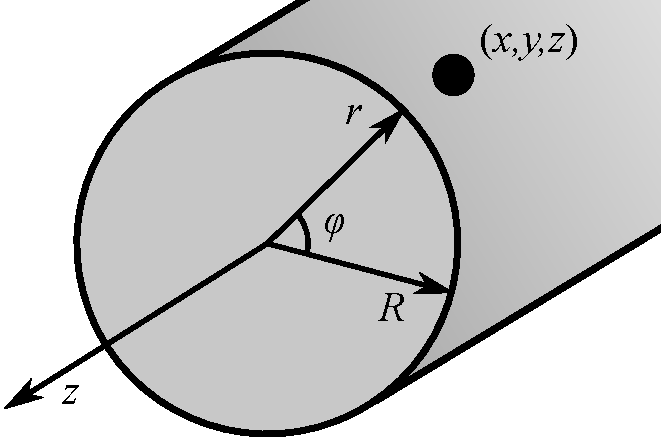
\includegraphics[width = .72\columnwidth]{Analytisk-Mekanik/cylinderopg_sh.pdf}
\caption{Partikel på cylinder.} \label{cyl-fig}
\end{figure}
%
%
\begin{opgave}{Partikel på en cylinder}{1} \label{opg:Cylinder}
Vi ser på en partikel, der kan bevæge sig frit på overfladen af en cylinder med radius $R$, som det ses på figur \ref{cyl-fig}. Her er det oplagt at bruge cylindriske koordinater:
\begin{align*}
x &= r\cos(\phi) \, , \\
y &= r\sin(\phi) \, , \\
z &= z \, .
\end{align*}
\opg Brug de cylindriske koordinater som generaliserede koordinater. Hvilke koordinater ændres, når partiklen bevæger sig?
\opg Udregn $\dt x$, $\dt y$ og $\dt z$ i de nye koordinater.
\opg Opstil den kinetiske energi, $K=\frac{1}{2}mv^2$.
\opg Opstil Lagrangefunktionen. Den potentielle energi er altid nul.
\opg Brug Euler-Lagrangeligningerne til at opstille anden ordens differentialligninger, for de koordinater der ændres, når partiklen bevæger sig.
\opg Hvordan bevæger partiklen sig?
\end{opgave}
%
%
\begin{figure}[h!]
	\centering
	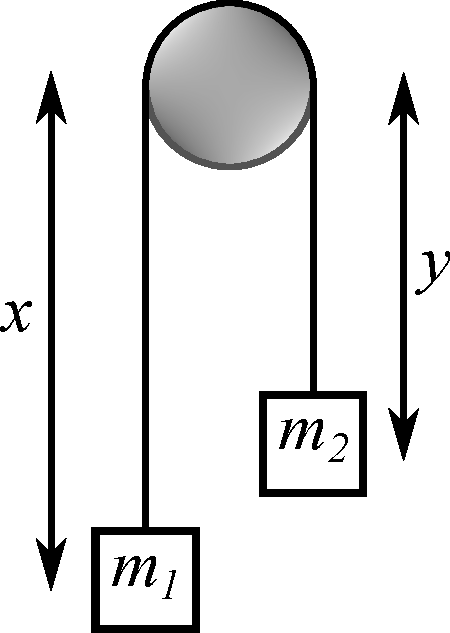
\includegraphics[width=.65\columnwidth]{Analytisk-Mekanik/Atwood.pdf}
	\caption{Illustration af Atwoods faldmaskine, hvor to lod forbindes med en snor over en trisse.} \label{fig:Atwood}
\end{figure}
%
%
\begin{opgave}{Atwoods faldmaskine}{1} \label{opg:Atwood}
I figur \ref{fig:Atwood} ses en illustration af Atwoods faldmaskine, hvori to lodder hænges i hver sin ende af en snor med konstant længde $l$. I figuren er to koordinater også defineret, og de to lodders masser er indtegnet.
\opg Argumenter for at der kun er ét generaliseret koordinat, og udtryk $y$ ved $x$.
\opg Udtryk $\dt{y}$ ved $\dt{x}$.
\opg Definer hhv. $x = 0$ og $y = 0$ som nulpunkt for den potentielle energi for hvert lod, og opskriv den totale potentielle energi\footnote{Har man svært ved at acceptere gyldigheden af at regne med negativ potentiel energi, kan man godt definere nulpunktet under faldmaskinen, hvilket gør at Lagrangefunktionen kommer til at indeholde nogle ekstra konstanter.}.
\opg Opskriv den kinetiske energi som summen af den kinetiske energi for hver af de to lodder.
\opg Vis at Lagrangefunktionen for systemet kan skrives på formen
\begin{align*}
	L(x,\dt{x},t) &= \frac{1}{2}(m_1+m_2)\dt{x}^2 \\
	&+ g\Big(m_1x + m_2(l-x-\pi R)\Big) \: .
\end{align*}
\opg Vis ved brug af Euler-Lagrangeligningen, at systemets bevægelsesligning er
\begin{align*}
	\ddt{x} = g\frac{m_1-m_2}{m_1+m_2} \: .
\end{align*}
\opg Vis ud fra bevægelsesligningen, hvad fortegnet af $\ddt{x}$ er afhængigt af om $m_1>m_2$ eller $m_2>m_1$. Hvilket af de to lodder vil falde ned (hvad betyder det for retningen af bevægelsen)?\\ 
Skrives bevægelsesligningen lidt om fås
\begin{align*}
	\dif[2]{t}{x} &= g\frac{m_1-m_2}{m_1+m_2} = a \\
	\implies \dif{t}{} \left( \dif{t}{x} \right) &= a \\
	\implies \dif{t}{x} &= \ubint{a}{t}\\
	\implies x(t) &= \ubiint{a}{t}{t}
\end{align*}
Det trick vi bruger her er, at integration og differentiation er hinandens omvendte operationer ligesom plus og minus er hinandens omvendte operationer.\footnote{Faktisk har vi også antaget, at to integrationskonstanter er $0$, men det er en mindre detalje.} 
\opg Bestem $x(t)$ ved ovenstående integral.\\ 
Hint: Regn det inderste integrale, så det yderste.
\end{opgave}
%
%
\begin{opgave}{Yoyo}{1} \label{opg:Yoyo}
Betragt yoyoen i figur \ref{fig:yoyo} med massen $m$ og de fysiske dimensioner som vist i figuren.
%
\begin{figure}[]
	\centering
	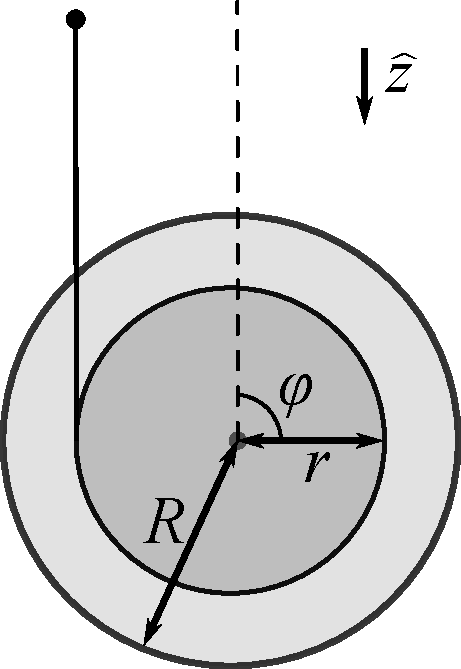
\includegraphics[width=.61\columnwidth]{Analytisk-Mekanik/yoyo.pdf}
	\caption{Skitse af en simpel yoyomodel med radier $r$ og $R$ i et tyngdefelt med i nedadgående retning med styrken $g$.} \label{fig:yoyo}
\end{figure}
%
Tyngdekraften har størrelsen $g$ i $z$-retningen, $\v{F}_\mathrm{g} = mg\zhat$, og den ideelle snor sidder fast i afstanden $r$ fra centrum. At snoren er ideel betyder, at den anses som ustrækkelig, masseløs, og derudover anses friktionen mellem snoren og yoyoen som værende så stor, at yoyoen ikke glider. Det kan vises, at yoyoens inertimoment i denne model er
\begin{align*}
	I = \frac{1}{2}mR^2 \: .
\end{align*}
Som generaliseret koordinat benyttes $z$, fordi $z$ og $\phi$ er koblede.
\opg Antagelsen at friktionen mellem snoren og yoyoen er tilpas stor, gør at det punkt hvor snoren slipper yoyoen står stille, hvilket betyder, at rotationen lige præcis udligner bevægelsen fra, at yoyoen falder nedad.\footnote{Dette kaldes ofte at yoyoen \textit{ruller uden at glide}, hvilket er en meget almindelig antagelse i fysik.} Det betyder, at farten $v$ i ligning \eqref{k-eq:SmartFart} er lig med farten $v_\textsc{cm}$ i ligning \eqref{k-eq:K}, hvor begge ligninger henviser til kompendiet. Brug disse ligninger til at vise at
\begin{align*}
	K = \frac{1}{2}m\dt{z}^2 + \frac{1}{4}mR^2\left(\frac{\dt{z}}{r}\right)^2 \: .
\end{align*}
\opg Argumenter for at den potentielle energi kan skrives på formen $V = -mgz$.
\opg Konkluder at Lagrangefunktionen for problemet er
\begin{align*}
	L = \frac{1}{2}m\left[1 + \frac{1}{2}\left(\frac{R}{r}\right)^2\right]\dt{z}^2 + mgz \: .
\end{align*}
\opg Bestem nu følgende afledede af Lagrangefunktionen
\begin{align*}
	\pdif{z}{L} &= \; ? \\
	\pdif{\dt{z}}{L} &= \; ? \\
	\el{\dt{z}} &= \; ?
\end{align*}
\opg Brug Euler-Lagrangeligningen, ligning \eqref{k-Euler-Lagrange} i kompendiet, til at vise at
\begin{align} \label{eq:YoyoDiffLign}
	\ddt{z} = \frac{g}{1 + \frac{1}{2}\left(\frac{R}{r}\right)^2} \: .
\end{align} \\[1mm]
Det kan vises at løsningen til denne differentialligning er
\begin{align} \label{eq:YoyoBevLign}
	z(t) = \frac{g}{2}\left[1 + \frac{1}{2}\left(\frac{R}{r}\right)^2\right]^{-1}t^2 + v_0t + z_0 \: ,
\end{align}
hvor $v_0$ er startfarten, og $z_0$ er startstedkoordinatet. Ved indsættelse i ligning \eqref{eq:YoyoDiffLign} kan det vises, at ligning \eqref{eq:YoyoBevLign} er en løsning, eller det kan udledes med samme metode som i opgaverne \ref{opg:Atwood} og \ref{opg:cylinder}.
\opg Overvej hvilke fordele og ulemper der er, ved at benytte Lagrangemekanikken til at løse dette problem frem for Newtonsk mekanik.
\end{opgave}
%
%
\begin{opgave}{Klods på en fjeder}{2}
I starten af kompendiets første kapitel blev det vist, at bevægelsesligningen for en klods på en fjeder, figur \ref{k-fig:fjeder} i kompendiet, er
\begin{align*}
	\ddt{x} = -\frac{k}{m}x \: .
\end{align*}
Til dette blev Newtons formulering af mekanikken brugt, men det samme kan også opnås med Lagrangeformalismen.
\opg Opstil Lagrangefunktionen for problemet.
\opg Benyt Euler-Lagrangeligningen til at komme frem til det samme.
\end{opgave}
%
%
\begin{opgave}{Cylinder på skråplan}{2}\label{opg:cylinder}
En cylinder med massen $m$, radius $R$ og inertimoment $I$ placeres på et skråplan med vinklen $\alpha$ i forhold til vandret.\\
\opg Skitser situationen.
\opg Indtegn på skitsen det koordinatsystem, der giver det færrest mulige afhængige koordinater.
\opg Opstil den potentielle energi $V$ for systemet, hvor der ses bort fra cylinderes udtrækning.
\opg Udtryk den kinetiske energi $K$ ved cylinderens fysiske parametre og tidsafledede af de valgte generaliserede koordinater.
\opg Opskriv problemets Lagrangefunktion.
\opg Vis at ved løsning af Euler-Lagrangeligningen fåes
\begin{align*}
\ddt{x} = -\dfrac{g\sin\alpha}{1+I/mR^2} \: .
\end{align*}
\opg Argumenter for at accelerationen er konstant.
\opg Lad nu accelerationen være $\tilde{g}$, og vis at bevægelsesligningens løsning er
\begin{align*}
x(t) = \frac{1}{2}\tilde{g}t^2 + v_0t + x_0 \: .
\end{align*}
\end{opgave}
%
%
\begin{figure}[h!]
	\centering
	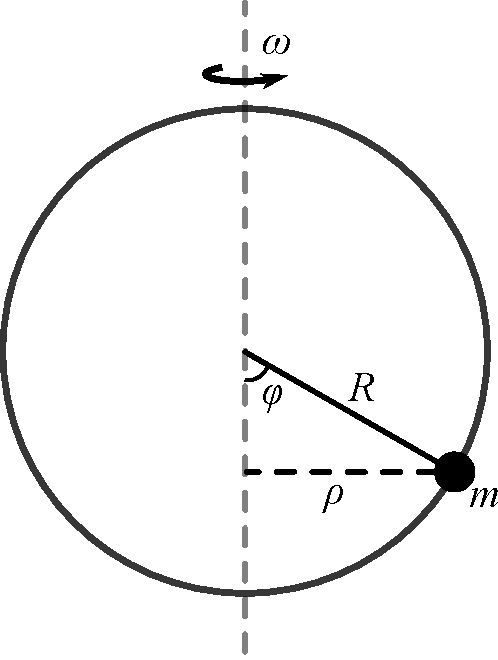
\includegraphics[width=.65\columnwidth]{Analytisk-Mekanik/BeadOnHoop.pdf}
	\caption{Illustration af situationen, hvor koordinater og andre parametre er indtegnet.} \label{fig:BeadOnHoop}
\end{figure}
%
%
\newpage
\begin{opgave}{Masse på roterende ring}{3}
Et lod med masse $m$ er placeret på en ring, hvorpå den kan bevæge sig friktionsløst, som i figur \ref{fig:BeadOnHoop}. Ringen har radius $R$, og den roterer om sin egen akse med vinkelhastigheden $\omega$. Massen kan beskrives udelukkende ved det generaliserede koordinat $\phi$, men for at indse dette gøres brug af koordinatet $\rho$.
\opg Udtryk den potentielle energi ved det generaliserede koordinat $\phi$, således at $V(\phi=0)=0$.
\opg Massens hastighed deles nu op i to komponenter - en der svarer til ind i tegningen og en langs ringen. Disse kaldes henholdsvis $v_\mathrm{ring}$, idet det er bevægelsen som følge af ringens rotation, og $v_\mathrm{lod}$ idet det er lodets bevægelse på ringen. Bestem disse komponenter udtrykt ved $\omega$, $\phi$ og $\dt{\phi}$, samt eventuelle geometriske parametre.\\
Hint: Benyt ligning \eqref{k-eq:SmartFart} i kompendiet.
\opg Brug dette til at bestemme den kinetiske energi, og vis dermed at Lagrangefunktionen er
\begin{align*}
	L = \frac{1}{2}mR^2\big[\dt{\phi}^2 + \omega^2\sin^2(\phi)\big] - mgR\big[1-\cos(\phi)\big] \: .
\end{align*}
\opg Benyt Euler-Lagrangeligningen til at vise, at bevægelsesligningen er
\begin{align*}
	\ddt{\phi} = \left[\omega^2\cos(\phi) - \frac{g}{R}\right]\sin(\phi) \: .
\end{align*}
\opg Hvad er kriteriet for henholdsvis et stabilt og ustabilt ligevægtspunkt fysisk og matematisk?
\opg Brug kriterierne til at bestemme systemets ligevægtspunkter, og forklar hvad de betyder fysisk.
\opg Eksister alle disse punkter for alle $\omega, R$ og $g$?
\opg Diskuter om ligevægtspunkterne er stabile eller ustabile i alle tilfælde fra sidste spørgsmål.\footnote{Ligevægtspunkterne $\phi_0 = 0,\pm\pi$ er ikke super komplicerede at vise stabiliteten af matematisk, men det sidste er svært, hvorfor dette bør tilgås med forsigtighed. Det er dog vist i facitlisten, hvordan dette gøres, hvilket kan være en gennemlæsning værd.}
\end{opgave}
%
%
\section*{Flerlegemeproblemer}
%
%
\begin{figure}[h!]
\centering
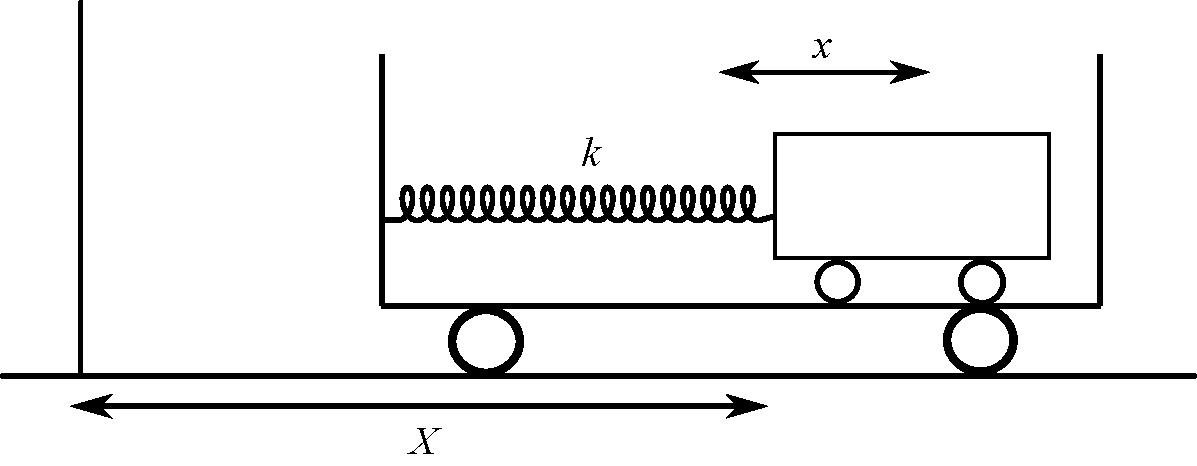
\includegraphics[width=\columnwidth]{Analytisk-Mekanik/ToKobledeVogne.pdf}
\caption{Illustration af problemet i opgave \ref{opg:ToKobledeVogne}. $X$ er stedkoordinatet for den store vogn, og $x$ er stedkoordinatet for den lille, hvor $x=0$ defineres som midtpunktet i den store vogn.}
\label{fig:ToKobledeVogne}
\end{figure}
%
%
\begin{opgave}{To koblede vogne}{2} \label{opg:ToKobledeVogne}
En lille vogn med massen $m$ placeres i en større vogn, og de to forbindes med en fjeder med fjederkonstant $k$. Den lille vogn antages at kunne bevæge sig friktionsløst i forhold til den store og den store i forhold til underlaget, og de generaliserede koordinater defineres som på figur \ref{fig:ToKobledeVogne}. Den store vogn tvinges til simpel harmonisk bevægelse, det vil sige $X = A\cos(\omega t)$, hvor $A,\omega$ er konstanter, og derudover kaldes den lille vogns naturlige vinkelfrekvens $\omega_0 = \sqrt{\frac{k}{m}}$.
\opg Argumenter for at den lille vogns hastighed i forhold til underlaget kan skrives som
\begin{align*}
v = \dt{x} + \dt{X} \: ,
\end{align*}
og brug dette til at indse, at
\begin{align*}
K = \frac{1}{2}m\left(\dt{x} + \dt{X}\right)^2 \: .
\end{align*}
\opg Argumenter for at den potentielle energi for den lille vogn er
\begin{align*}
V = \frac{1}{2}kx^2 \: ,
\end{align*}
og konkluder at
\begin{align*}
L = \frac{1}{2}m\left(\dt{x} + \dt{X}\right)^2 - \frac{1}{2}kx^2 \: .
\end{align*}
\opg Brug dette til at vise, at
\begin{align*}
\pdif{\dt{x}}{L} &= m(\dt{x} + \dt{X}) \: ,\\
\pdif{x}{L} &= -kx \: .
\end{align*}
\opg Vis at
\begin{align*}
\dif{t}{}\left(\pdif{\dt{x}}{L}\right) = m\ddt{x} - Am\omega^2\cos(\omega t) \: ,
\end{align*}
og konkluder at
\begin{align*}
\ddt{x} + \frac{k}{m}x = A\omega^2\cos(\omega t) \: .
\end{align*}
\opg Fastholdes den store vogn nu i $X=0$ bliver systemet i denne opgave ækvivalent til et system, uden den store vogn, hvor fjederen på den lille vogn er spændt fast på væggen, hvilket er en harmonisk oscillator. $X=0$ kan realiseres ved at sætte $A=0$. Vis at bevægelsesligningen i dette tilfælde reducerer til en harmonisk oscillator.
\opg Hvorfor er det relevant at tjekke at systemet reducerer til en harmonisk oscillator i grænsen $A=0$?\\ \\
\end{opgave}
%
%
\begin{figure}[h!]
\centering
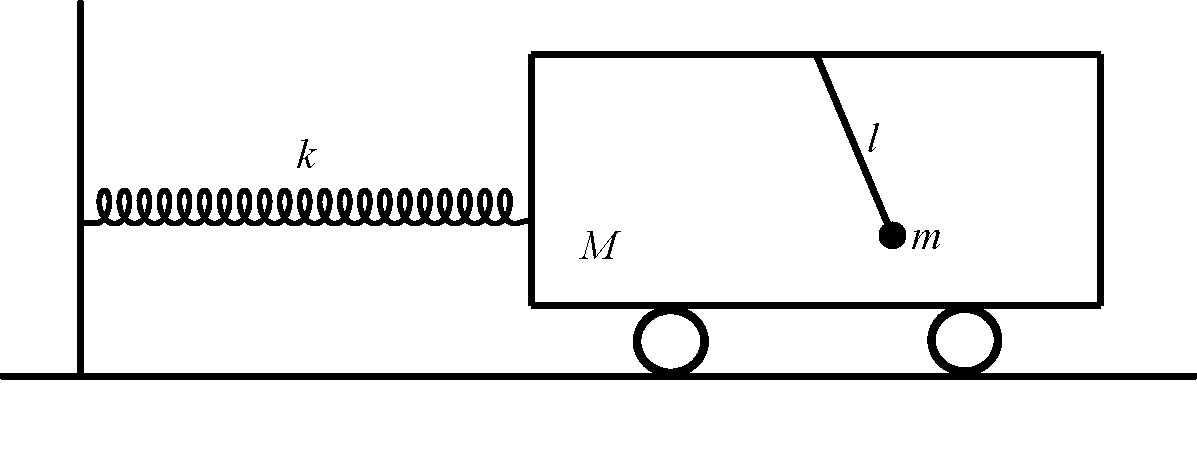
\includegraphics[width=\columnwidth]{Analytisk-Mekanik/PendulIVognOpg.pdf}
\caption{Pendul med massen $m$ og længden $l$ placeret i en vogn med massen $M$, der er fastgjort til en væg med en en fjeder med fjederkonstant $k$.}
\label{fig:PendulIVognOpg}
\end{figure} 
%
%
\begin{opgave}{Pendul i en vogn}{4}
I figur \ref{fig:PendulIVognOpg} er der tegnet et pendul, ophængt i en vogn, der tilmed er fastspændt med en fjeder til en væg, og de relevante fysiske størrelser er indtegnet.
\opg Identificer systemets generaliserede koordinater, indtegn enhedsvektorerne for et kartesisk koordinatsystem og definer origo. %(hint: Se beskrivelsen af pendulet med Lagrangeformalismen og opgave \ref{opg:ToKobledeVogne})
\opg Opskriv pendulets kartesiske koordinater, $(X_p,Y_p)$, udtrykt ved de generaliserede koordinater, samt vognens kartesiske $X$-koordinat, $X_v$, og argumenter for, at $Y_v$ er ubetydelig for problemet.
\opg Bestem systemets potentielle energi.
\opg Bestem systemets kinetiske energi og opskriv Lagrangefunktionen. %(hint: Anvend de kartesiske koordinater fra sidste opgave til først at bestemme de relevante hastigheder)
\opg Vis at løsningen til Euler-Lagrangeligningen er de koblede differentialligninger
\begin{align*}
a&) \quad M\ddt{x} + m\ddt{x} + ml\ddt{\phi}\cos\phi - ml\dt{\phi}^2\sin\phi = -kx \:, \\
b&) \quad ml^2\ddt{\phi} + ml\ddt{x}\cos\phi = -mgl\sin\phi \: .
\end{align*}
\opg Bestem Taylorudviklingen til 1. orden i $\phi$ af bevægelsesligningerne. \\ \\
Nu kigges på grænserne
\begin{align*}
&1. \quad k \rightarrow \infty \: ,\\
&2. \quad M \gg m \: .
\end{align*}
\opg Hvilken fysisk situation svarer hver grænse til?
\opg Hvad forventes systemet at blive til i de ovenstående grænser?
\opg Hvad bliver det til?
\end{opgave}
\newpage
%
%
\section*{Fiktive Kræfter}
%
%
\begin{opgave}{Fysiske og fiktive kræfter}{2} \label{opg:Fiktivekraefter}
Nu betragtes systemet fra karruseleksemplet i afsnit \ref{k-sec:Karrusel}, og der tilføjes en stedafhængig kraft til systemet med potentiel energi $V(x,y)$.
\opg Hvorfor giver antagelserne at følgende er sandt?
\begin{align*}
	\pdif{\dt{x}}{}V(x,y) &= 0 \\
	\pdif{\dt{y}}{}V(x,y) &= 0
\end{align*}
\opg Argumenter for at $V(x,y)$ ikke indgår i $\el{\dt{q}_i}$ for $q_i=x,y$. Med andre ord, at
\begin{align*}
	\el{\dt{x}} &= \dif{t}{}\left(\pdif{\dt{x}}{K}\right) \: , \\
	\el{\dt{y}} &= \dif{t}{}\left(\pdif{\dt{y}}{K}\right) \: .
\end{align*}
\opg Konkluder at bevægelsesligningerne for systemet er
\begin{align*}
	m\ddt{x} &= 2m\omega\dt{y} + m\omega^2x -\pdif{x}{}V(x,y) \: , \\
	m\ddt{y} &= -2m\omega\dt{x} + m\omega^2y -\pdif{y}{}V(x,y) \: ,
\end{align*}
som kan skrives på formen
\begin{align*}
	m\ddt{x} &= F_x^\mathrm{cor} + F_x^\mathrm{cf} - \pdif{x}{}V(x,y,z) \: , \\
	m\ddt{y} &= F_y^\mathrm{cor} + F_y^\mathrm{cf} - \pdif{y}{}V(x,y,z) \: .
\end{align*}
hvor superscriptet angiver, hvilken af de to fiktive kræfter, der er tale om, og subscriptet angiver retningen.
\opg Beskriv hvordan disse fiktive kræfter opfører sig overfor Newtons 2. lov og sammenlign med fysiske kræfter som for eksempel tyngdekraften. \vspace{3mm}\\
Det vigtige i denne opgave er ikke at regne eksemplet igennem på ny, men at gennemgå argumenterne for de konklusioner der drages, for at give en forståelse for begrebet \textit{fiktive kræfter}.
\end{opgave}
%
%
\begin{figure*}
	\centering
	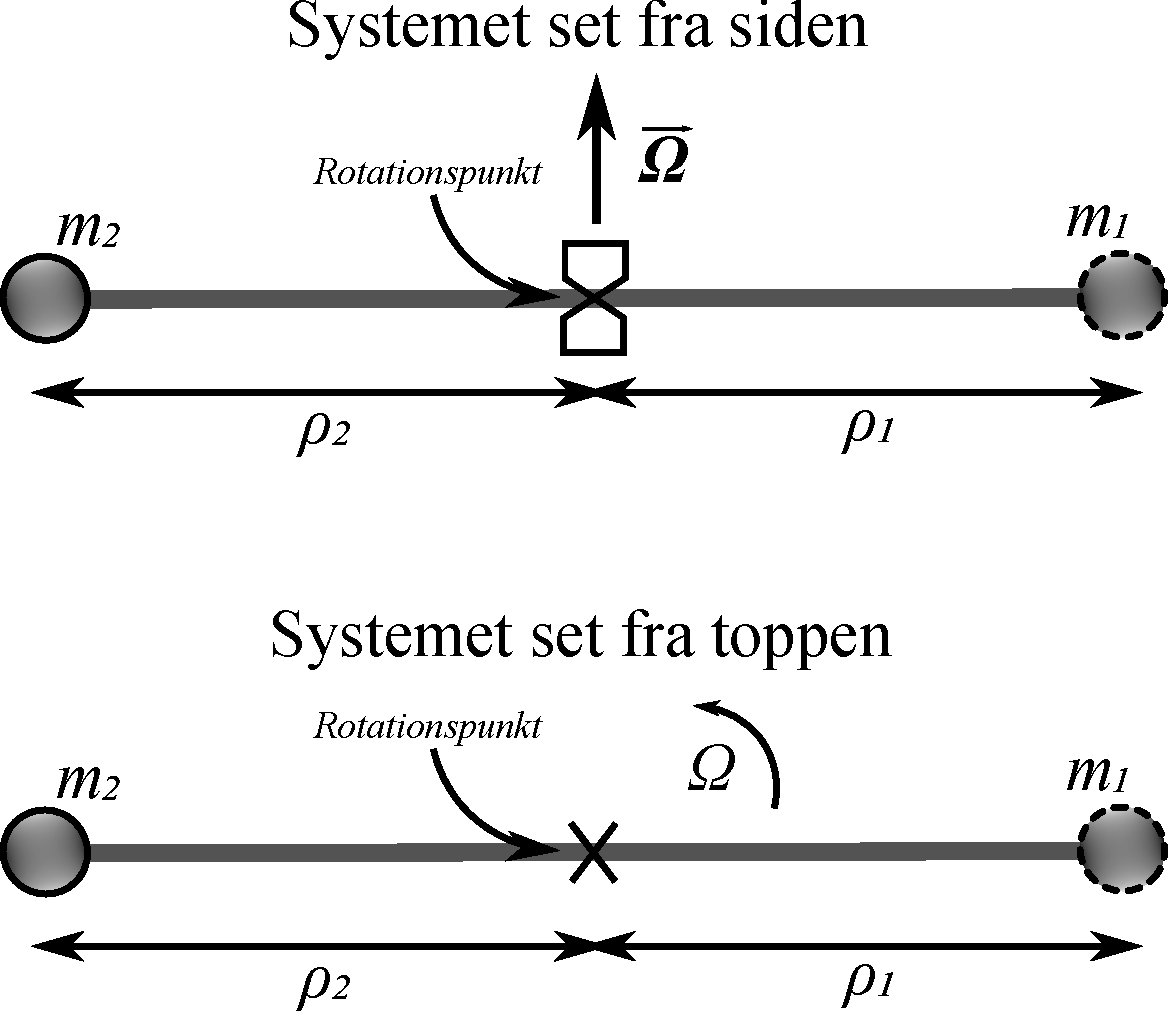
\includegraphics[width=.67\textwidth]{Analytisk-Mekanik/ToMasserRoterendeStang.pdf}
	\caption{Illustration af problemet, hvor stangen kan bevæge sig lineært gennem rotationspunktet udover at rotere med konstant vinkelhastighed $\Omega$.}	\label{fig:ToMasserRoterendeStang}
\end{figure*}
%
%
\begin{opgave}{To masser på en roterende stang}{3}
To legemer med masserne $m_1$ og $m_2$ fastspændes for enden af en stang. Denne stang monteres på et apparat, således at stangen kan rotere omkring apparatet med konstant vinkelhastighed $\v{\Omega}$, samtidig med at den kan bevæge sig friktionsløs frem og tilbage gennem apparatet. Afstanden fra legemerne til apparatet kaldes hhv. $\rho_1$ og $\rho_2$, og da vil $l = \rho_1 + \rho_2$, hvor $l$ er længden af stangen. Opstillingen kan ses på figur~\ref{fig:ToMasserRoterendeStang}.
\opg Identificer et logisk koordinatsystem at beskrive problemet i.
\opg Identificer de(n) generaliserede koordinat(er) for hvert legeme.
\opg Antagelserne giver en begrænsning af hvordan de to legemer kan bevæge sig i forhold til hinanden. Hvad er sammenhængen mellem de to legemers hastighed?
\opg Med henvisning til ligning \eqref{k-eq:FiktiveKraefter} i kompendiet bestem Coriolis og centrifugalkraften på hvert legeme, og inkluder begrænsningen på hastighederne.
\opg Tegn kræfterne der virker på hvert legeme, og beskriv hvilke antagelse tegningen bygger på.
\opg Argumenter for at Corioliskraften er ubetydelig for problemet grundet antagelserne.
\opg Benyt at summen af kræfter på et legeme i ligevægt er nul, $\sum\v{F} = \v{0}$, til at bestemme et systemets ligevægtskonfiguration.
\opg Hvordan forventes ligevægtskonfigurationen at se ud, under antagelse af at $m_1 = m_2$.
\opg Stemmer forventningen og det beregnede udtryk overens?
\end{opgave}
%
%
\begin{opgave}{Er fiktive kræfter trælse?}{3}
Betragt nu de fiktive kræfter, som givet i ligning \eqref{k-eq:FiktiveKraefter} i kompendiet.
\opg Afhænger hver af de fiktive kræfter af sted eller hastighed?
\opg Det er bøvlet, hvis eksempelvis funktionen indgår som sig selv, samt sin første og anden afledede. Med tanke på hvad de kræfter, der er arbejdet mest med i kapitlet, giver nogle af de fiktive kræfter så anledning til differentialligninger, der er specielt vanskelige at løse?
\opg Hvis differentialligningen kan skrives på formen
\begin{align*}
\dif[2]{t}{f(t)} = k\dif{t}{f(t)}
\end{align*}
kan den relativt simpelt løses. Hvorfor?
\end{opgave}
%
%
\section*{Perspektiverende Problemer}
%
%
\begin{opgave}{Tennis Racket Theorem}{4}
Indtil videre har vi kun kigget på rotationer om én akse, men ofte roterer ting om flere akser, hvilket komplicerer tingene en hel del. I denne opgave vil vi ikke forsøge at udlede bevægelsesligningerne for et sådant system, men forsøge at forstå hvilken information de kan give os. Det kan vises at bevægelsesligningerne for et stift legeme, der kan rotere om tre akser med hver sit inertimoment er
\begin{align*}
	I_x\dt{\omega}_x &= (I_y-I_z)\omega_y\omega_z \: , \\
	I_y\dt{\omega}_y &= (I_z-I_x)\omega_z\omega_x \: , \\
	I_z\dt{\omega}_z &= (I_x-I_y)\omega_x\omega_y \: ,
\end{align*}
eller på vektorform
\begin{align} \label{eq:TRT_DiffLign}
	\xyz{I_x\dt{\omega}_x}{I_y\dt{\omega}_y}{I_z\dt{\omega}_z} = \xyz{(I_y-I_z)\omega_y\omega_z}{(I_z-I_x)\omega_z\omega_x}{(I_x-I_y)\omega_x\omega_y} \: .
\end{align}
Her er $I_i$ og $\omega_i$ henholdsvis inertimomentet og vinkelhastigheden for rotation om den $i$'te akse, og yderligere antages det at $I_x>I_y>I_z>0$.
\opg Antag at $\omega_y \approx \omega_z$ er meget små og brug dette til at vise, at
\begin{align} \label{eq:TRT_DiffLignX}
	\dif{t}{}\xyz{I_x\dt{\omega}_x}{I_y\dt{\omega}_y}{I_z\dt{\omega}_z} \simeq \xyz{0}{(I_z-I_x)\dt{\omega_z}\omega_x}{(I_x-I_y)\omega_x\dt{\omega}_y} \: .
\end{align}
Hint: $\omega_y$ og $\omega_z$ er så små, at andenordensled med dem, dvs. led på formen $\omega_i\omega_j$ hvor $i=y,z$ og $j=y,z$, er nul, mens førsteordensled ikke er.
\opg Vis ved brug af ligningerne \eqref{eq:TRT_DiffLign} og \eqref{eq:TRT_DiffLignX}, at
\begin{align} \label{eq:TRT_DDiffLignX}
	\dif{t}{}\xyz{I_x\dt{\omega}_x}{I_y\dt{\omega}_y}{I_z\dt{\omega}_z} \simeq \xyz{0}{\omega_x^2\omega_y(I_z-I_x)(I_x-I_y)/I_z}{\omega_x^2\omega_z(I_x-I_y)(I_z-I_x)/I_y} \: .
\end{align}
\opg Konkluder ud fra ligning \eqref{eq:TRT_DDiffLignX} at fortegnet for $\ddt{\omega}_y$ og $\ddt{\omega}_z$ er modsat af henholdsvis $\omega_y$ og $\omega_z$.
\opg Antag nu at $\omega_x \approx \omega_z$ er meget små, analogt til spørgsmål 1), og brug helt samme metode til at vise, at
\begin{align} \label{eq:TRT_DiffLignY}
	\dif{t}{}\xyz{I_x\dt{\omega}_x}{I_y\dt{\omega}_y}{I_z\dt{\omega}_z} \simeq \xyz{\omega_y^2\omega_x(I_y-I_z)(I_x-I_y)/I_z}{0}{\omega_y^2\omega_z(I_x-I_y)(I_y-I_z)/I_x} \: .
\end{align}
\opg Benyt nu ligning \eqref{eq:TRT_DiffLignY} til at konkludere, at fortegnene for $\ddt{\omega}_x$ og $\omega_x$ er ens og ligeledes for $\omega_z$.
\opg Legemet sættes til at rotere om sin $i$'te akse, hvor vinkelhastigheden om de andre akser er små. Hvis legemet fortsætter med stort set kun at rotere om den $i$'te akse, da betragtes rotation om den $i$'te rotationsakse som stabil. Argumenter for at rotation om den $i$'te rotationsakse er stabil, hvis $\ddt{\omega}_j \propto - \omega_j \, \forall \, j\neq i$.
\opg Ved analoge udregninger fås, at $\ddt{\omega}_x \propto -\omega_x$ og $\ddt{\omega}_y \propto -\omega_y$ hvis $\omega_x\approx\omega_y$ er små. Konkluder at rotation om $x$- og $z$-aksen er stabil, mens rotation om $y$-aksen er ustabil. Dette resultat kaldes \textit{Tennis Racket Theorem}, \textit{Intermediate Axis Theorem} eller \textit{Dzhanibekov Effect}\footnote{Løses differentialligningen i ligning \ref{eq:TRT_DiffLign} fås en bevægelse som denne: \url{https://www.youtube.com/watch?v=1n-HMSCDYtM}} efter Dzhanibekov, der bemærkede det under en mission i rummet.
\opg Den eneste antagelse der er lavet, er at legemet er stift\footnote{Det er også antaget at legemet ikke er påvirket af ydre kræfter i udledningen af ligning \ref{eq:TRT_DiffLign}, men det betyder bare at konklusionen om stabilitet af rotationsakser ikke afhænger af nogle ydre kræfter.}. Brug dette til at undersøge dette fænomen med virkelige objekter, forklar hvilke rotationsakser, der er mulige for objektet, samt den relative størrelse af inertimomentet for rotation omkring de forskellige akser.
\end{opgave}
%
%
\begin{opgave}{Hamiltonfunktionen og et systems energi}{3} \label{opg:HamiltonEnergi}
Antag at et systems kinetiske energi kan skrives på formen $K = \frac{1}{2}A(q)\dt{q}^2$, hvor $A(q)$ er en arbitrær funktion af $q$, som er det eneste generaliserede koordinat. Den potentielle energi kaldes $V(q)$, og der antages kun, at den er stedsafhængig.
\opg Opskriv systemets Lagrangefunktion.
\opg Bestem den generaliserede impuls ud fra dennes definition.
\opg Udtryk $\dt{q}$ ved $p$ og $A(q)$.
\opg Benyt definitionen af Hamiltonfunktion til at bestemme denne.
\opg Vis at hvis et systems kinetiske energi kan skrives på formen $K = \frac{1}{2}A(q)\dt{q}^2$, så er $H = E$.
\opg Argumenter for at disse argumenter generaliserer til $n$ generaliserede koordinater, hvor den kinetisk energi på tilsvarende vis antages at være
\begin{align*}
	K = \sum_i\frac{1}{2}A(q_i)\dt{q}_i^2 \: .
\end{align*}
\end{opgave}
%
%
\begin{opgave}{Fra klassisk mekanik til kvantemekanik}{3}
Her vil sammenhængen mellem klassisk mekanik og kvantemekanik belyses gennem en metode til at opskrive Hamiltonoperatoren for et system, ved at starte med en klassisk analyse af problemet. Der kigges her på én partikel.
\opg Antag at den generaliserede impuls kan skrives på formen $p = m\dt{q}$. Benyt dette til at opskrive den kinetiske energi udtrykt ved impulsen $p$.
\opg Benyt resultatet fra opgave \ref{opg:HamiltonEnergi} til at opskrive systemets Hamiltonfunktion.
\opg For at kunne beskrive systemet kvantemekanisk, skal Hamiltonfunktionen skrives om til en Hamiltonoperator. Hvilke elementer i Hamiltonfunktionen skal omskrives, for at stå på operatorform?
\opg Omskriv de før angivne elementer til operatorform ved hjælp af tabel \ref{k-tab:operatorer_i_kvant} i kompendiet, og bestem derved Hamiltonoperatoren.
\end{opgave}
%
%
\begin{opgave}{Energibevarelse i Hamilton}{4}
I opgave \ref{opg:HamiltonEnergi} blev det vist at Hamiltonfunktionen i nogle tilfælde er lig med et systems energi. Det kunne derfor være interessant at undersøge, under hvilke omstændigheder Hamiltonfunktionen er bevaret over tid.
\opg Beskriv forskellen på den fuldstændige differentiation, f.eks. $\d/\d t$, og den partielle differentiation, eksempelvis $\partial/\partial t$. \footnote{Differentialoperatorerne er her skrevet med hensyn til tid, men det er bare for at give et eksempel. Der tænkes her på den generelle forskel.} 
\opg Opskriv den fuldstændigt tidsafledede af en generel Hamiltonfunktion af ét generaliseret koordinat, $\d H/\d t$, vha. kædereglen.
\opg Benyt nu Hamiltons ligninger til at simplificere summen.
\opg Konkluder at
\begin{align*}
\dif{t}{H} = \pdif{t}{H} \: .
\end{align*}
\opg Under hvilke omstændigheder er Hamiltonfunktionen bevaret i tid?
\opg Med henvisning til opgave \ref{opg:HamiltonEnergi}, hvad betyder det fysisk for systemet, at Hamiltonfunktionen er bevaret i tid?
\opg Opskriv $\d H/\d t$ for en generel Hamiltonfunktion af $n$ generaliserede koordinater, og vis at ovenstående er sandt for $n$ generaliserede koordinater.
\end{opgave}
\documentclass[crop=false, class=memoir]{standalone}

\usepackage[utf8]{inputenc}%Nødvendig for danske bogstaver
\usepackage[danish]{babel}%Sørger for at ting LaTeX gør automatisk er på dansk
\usepackage{csquotes}
\usepackage{geometry}%Til opsætning af siden
\geometry{lmargin = 2.5cm,rmargin = 2.5cm}%sætter begge magner
\usepackage{lipsum}%Fyldtekst, til brug under test af layoutet
\usepackage{float}
\usepackage{graphicx}%Tillader grafik
\usepackage{epstopdf}%Tillader eps filer
\usepackage{marginnote}% Noter i margen
\interfootnotelinepenalty=10000 %undgår at fodnoter bliver spilittet op.
\usepackage[sorting=none]{biblatex}
\addbibresource{litteratur.bib}
\usepackage[hidelinks]{hyperref}%Tillader links
\usepackage{subcaption} % Tillader underfigurer
\usepackage[font={small,sl}]{caption}	% Caption med skrå tekst ikke kursiv

\usepackage{xcolor} %Bruges til farver
\usepackage{forloop} %Bruges til nemmere for loops

\newcounter{opgave}[chapter] %Definerer opgavenumrene og hvornår de nulstilles
\renewcommand{\theopgave}{\thechapter.\arabic{opgave}} %Definerer udseende af opgavenummereringen
\newcounter{delopgave}[opgave] %Definerer delopgavenumrene
\newcounter{lvl} %Definerer en "variabel" til senere brug

\definecolor{markerColor}{rgb}{0.0745098039, 0.262745098, 0.584313725} %Definerer farven af markøren
\newcommand{\markerSymbol}{\ensuremath{\bullet}} %Definerer tegnet for markøren
\newlength{\markerLength} %Definerer en ny længde
\settowidth{\markerLength}{\markerSymbol} %Sætter den nye længde til bredden af markøren

\newenvironment{opgave}[2][0]{%Definerer det nye enviroment, hvor sværhedsgraden er den første parameter med en default på 0
\newcommand{\opg}{\refstepcounter{delopgave}\par\vspace{0.1cm}\noindent\textbf{\thedelopgave)\space}}%Definerer kommando til delopgave
\refstepcounter{opgave}%Forøger opgavenummer med 1 og gør den mulig at referere til
\setcounter{lvl}{#1}%Sætter "variablen" lvl lig med angivelsen af sværhedsgraden
\noindent\hspace*{-0.75em}\hspace*{-\value{lvl}\markerLength}\forloop{lvl}{0}{\value{lvl}<#1}{{\color{markerColor}\markerSymbol}}\hspace*{0.75em}%Sætter et antal af markører svarende til sværhedsgraden
\textbf{Opgave \theopgave : #2}\newline\nopagebreak\ignorespaces}{\bigskip} %Angiver udseende af titlen på opgaverne samt mellemrummet mellem opgaver



\usepackage{mathtools}%Værktøjer til at skrive ligninger
\renewcommand{\phi}{\varphi}%Vi bruger varphi
\renewcommand{\epsilon}{\varepsilon}%Vi bruger varepsilon
\usepackage{physics}%En samling matematikmakroer til brug i fysiske ligninger
\usepackage{braket}%Simplere kommandoer til bra-ket-notation
\usepackage{siunitx}%Pakke der håndterer SI enheder godt
\DeclareSIUnit\clight{\text{\ensuremath{c}}} % Lysets fart i vakuum som c og ikke c_0
\usepackage{chemmacros}
\usechemmodule{isotopes}
\usepackage{tikz}
\usepackage[danish]{cleveref}
\usepackage{nicefrac}
% \renewcommand{\ref}[1]{\cref{#1}}
\creflabelformat{equation}{#2(#1)#3}
\crefrangelabelformat{equation}{#3(#1)#4 to #5(#2)#6}
\crefname{equation}{ligning}{ligningerne}
\Crefname{equation}{Ligning}{Ligningerne}
\crefname{section}{afsnit}{afsnitene}
\Crefname{section}{Afsnit}{Afsnitene}
\crefname{figure}{figur}{figurene}
\Crefname{figure}{Figur}{Figurene}
\crefname{table}{tabel}{tabellerne}
\Crefname{table}{Tabel}{Tabellerne}
\crefname{opgave}{opgave}{opgaverne}
\Crefname{opgave}{Opgave}{Opgaverne}
\crefname{delopgave}{delopgave}{delopgaverne}
\Crefname{delopgave}{Delopgave}{Delopgaverne}

\newcommand{\eqbox}[1]{\begin{empheq}[box=\fbox]{align}
	\begin{split}
	#1
	\end{split}
\end{empheq}}

\newcommand{\kb}{\ensuremath{k_\textsc{b}}}

\DeclareSIUnit{\parsec}{pc}
\DeclareSIUnit{\lightyear}{ly}
\DeclareSIUnit{\astronomicalunit}{AU}
\DeclareSIUnit{\year}{yr}
\DeclareSIUnit{\solarmass}{M_\odot}
\DeclareSIUnit{\solarradius}{R_\odot}
\DeclareSIUnit{\solarluminosity}{L_\odot}
\DeclareSIUnit{\solartemperature}{T_\odot}
\DeclareSIUnit{\earthmass}{M_\oplus}
\DeclareSIUnit{\earthradius}{R_\oplus}
\DeclareSIUnit{\jupitermass}{M_J}

% Infobokse og lignende
% http://mirrors.dotsrc.org/ctan/graphics/awesomebox/awesomebox.pdf
% \usepackage{awesomebox}


% Egen infobokse (virker kun med begrænsede symboler)

\usepackage[framemethod=tikz]{mdframed}
\usetikzlibrary{calc}
\usepackage{kantlipsum}

\usepackage[tikz]{bclogo}

\tikzset{
    % lampsymbol/.style={scale=2,overlay}
    % lampsymbol/.pic={\centering\tikz[scale=5]\node[scale=10,rotate=30]{\bclampe}}.style={scale=2,overlay}
    infosymbol/.style={scale=2,overlay}
}

\newmdenv[
    hidealllines=true,
    nobreak,
    middlelinewidth=.8pt,
    backgroundcolor=blue!10,
    frametitlefont=\bfseries,
    leftmargin=.3cm, rightmargin=.3cm, innerleftmargin=2cm,
    roundcorner=5pt,
    % skipabove=\topsep,skipbelow=\topsep,
    singleextra={\path let \p1=(P), \p2=(O) in ($(\x2,0)+0.92*(1.1,\y1)$) node[infosymbol] {\bcinfo};},
    % singleextra={\path let \p1=(P), \p2=(O) in ($(\x2,0)+0.5*(2,\y1)$) node[infosymbol] {\bcinfo};},
]{info}

% Skal bruges som
% \begin{info}[frametitle={Titel}]
%     Tekst
% \end{info}

\begin{document}

\chapter{Kvantemekanik}



\end{document}
\chapter{Exoplaneter} \label{cha:Astro}
\section{Introduktion} \label{exointro}
Et af de spørgsmål, der nok altid har optaget menneskeheden er, om vi er alene, eller der andre som os et sted? Engang var svaret ja - vi har mødt både neanderthalere og andre menneskearter gennem tiden. Men i alle områder, vi har undersøgt godt nok, kan vi ikke længere finde andre, der minder særligt meget om os selv mht. tænkemåde og teknologi. Et andet spørgsmål, der altid har optaget os er, hvordan vi og verden omkring os opstod. Er der andre steder som dette? Vi har kigget mod stjernerne og undret os over, hvad der findes langt borte.

Nu har vi endelig teknikken til at undersøge disse spørgsmål mere i dybden ved at lede efter exoplaneter, som er planeter uden for Solsystemet. Indtil videre har fokus ligget på at detektere så mange planeter som muligt og karakterisere dem, hvilket er nemmest for de store og tunge, men i fremtiden vil vi blive bedre til at analysere de jordlignende planeter. \\

%Astrointro om det observerbare univers, nukleosyntese og planetdannelse
\noindent
For at diskutere astrofysik, er det nyttigt at kende nogle begreber:\\

\noindent
\textbf{Luminositet} eller lysstyrke er den totale energi $E$ et objekt udsender i alle retninger per tid $t$.
\begin{align}
    L=\dif{t}{E}
\end{align}
\noindent
\textbf{Flux} beskriver hvor meget af noget man opfanger over et bestemt areal - sagt med andre ord, hvor meget der strømmer igennem et areal. Ofte siger man bare flux, når man egentlig mener energiflux - altså hvor meget af kildens energi vi opfanger. Fluxen $F$ måles i denne sammenhæng som energi $E$ per tid $t$ og areal $A$.
\begin{align}
    F=\frac{1}{A}\pdif{t}{E}
\end{align}
Det svarer til hvor meget af luminositeten, man opfanger over et bestemt areal, fx. på Jorden. Hvis man har et bestemt areal at måle med, og flytter det længere væk fra kilden, bliver det ramt af færre fotoner, så fluxen skal aftage. Fluxen følger
\begin{align}
    F=\frac{L}{4\pi D^2}, \label{afstandskv}
\end{align}
hvor $D$ er afstanden til objektet. Dette kaldes \emph{Afstandskvadratloven}, da fluxen falder med kvadratet på afstanden. Så objekter, der er langt væk, ser vi meget svagt. Afstandkvadratloven ser sådan ud, fordi man antager at stjerner udtråler isotropt, det vil sige lige meget i alle retninger, hvorfor den målte flux i en afstand $D$ fra kilden, er den fra kilden udsendt flux, over hvor stort et areal den har spredt sig over, hvilket er overfladen af en kugle.

\iffalse
    \textbf{Intensitet} er et mål for for meget lys der bliver udsendt i en bestemt retning. Det minder om flux, der bare også er divideret med hvor stor en vinkel af himlen man måler på. Vinklen $\d\Omega$ kaldes rumvinklen (solid angle på engelsk). 
    \begin{align}
        I=\frac{\partial^3E}{\partial t \partial A \partial\Omega}
    \end{align}
    Det interessante ved intensitet er, at det er uafhængigt af hvor langt man er fra kilden. Afstandskvadratloven siger at fluxen vil aftage, men til gengæld vil kilden også fylde mindre på himlen, og de effekter opvejer hinanden, så intensiteten bliver konstant.
\fi
\subsection{Dopplerforskydning}
Du kender nok til, at når en ambulance kører forbi, så lyder sirenens tone højere, når den nærmer sig, og dybere når den kører væk. Det skyldes et fænomen kaldet \emph{Dopplerforskydning}. %Find gerne lydklip til undervisningen
Det skyldes at lydbølgerne, eller mere præcist bølgens bølgelængde, skubbes sammen eller strækkes ud, afhængigt af hvilken hastighed de udsendes med i forhold til lytteren. Hvis en ambulance kører mod dig, og du står stille, vil du høre bølgerne sammenpresset. Men hvis du selv kører med samme hastighed foran ambulancen, så vil du høre dem på samme måde, som de bliver udsendt - altså på samme måde, som hvis både du og ambulancen står stille, da det er den relative hastighed, som er afgørende.
\begin{figure}[h!]
	\centering
	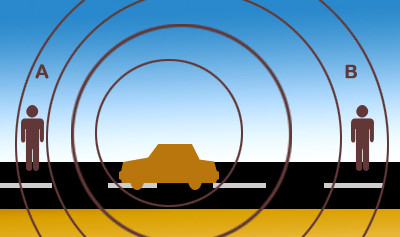
\includegraphics[width=0.5\textwidth]{Astrofysik/billeder/doppler.jpg}
	\caption{Dopplerforskydning af lyden fra en bil, der kører mod venstre. Person A vil høre en højere tone end person B, og personen i bilen vil høre noget et sted derimellem. Ringene viser et fast punkt på lydbølgerne.} % Kan man ikke ligeså godt skrive at ringene viser bølgetoppe, da det vel er dem man tegner pr. konvention?
	\label{doppler}
\end{figure}

Det samme sker for lys. Hvis en ambulance kører væk, vil både tonen blive dybere og lyset fra den en smule rødere, fordi bølgelængden bliver længere. Da rød svarer til lange bølgelængder og blå til korte (indenfor det synlige spektrum), så refererer rødforskydning til noget, som bevæger sig væk fra os og vice versa. 

Bemærk dog, at selvom fotoner og lydbølger har højere energi ved korte bølgelængder, så mister de ikke energi ved Dopplerforskydning - der er bare sket et skift i perspektivet, man ser bølgerne fra. Fra bølgens eget synspunkt (hvis man følger den) har den samme bølgelængde og energi hele tiden. På figur \ref{doppler} ses hvordan bølgerne "presses sammen" foran en kilde der bevæger sig, når man ser det fra et andet perspektiv.



\subsection{Spektre} \label{sec:spektrer}
Et spektrum viser intensiteten af lys ved forskellige bølgelængder eller frekvenser, fx som på figur \ref{spektrum}. Om bølger gælder det, at $v = f\lambda$, hvor $v$ er bølgens fart, $f$ er bølgens frekvens\footnote{Et andet almindeligt brugt symbol er det græske bogstav $\nu$, men her benyttes $f$, da det ikke minder så meget om det latinske bogstav $v$, der bruges om fart.} og $\lambda$ er bølgens bølgelængde. Lys bevæger sig med lysets fart, der afhænger af det medie lyset udbredes i, men det vigtige er, at den er kendt, hvorfor man simpelt kan regne $f$ ud fra $\lambda$ og omvendt. Pointen med dette er, at den eneste forskel på om et spektrum viser bølgelængde eller frekvens, er hvordan tallene skal fortolkes (fx vil spektret være spejlvendt, da de er omvendt proportionale).\footnote{For at gøre forvirringen total anvendes $\tilde{\nu} = \frac{1}{\lambda}$ også på nogle områder. Alt dette er traditioner og konventioner, der varierer fra område til område.} \\
\begin{figure}[h!]
	\centering
	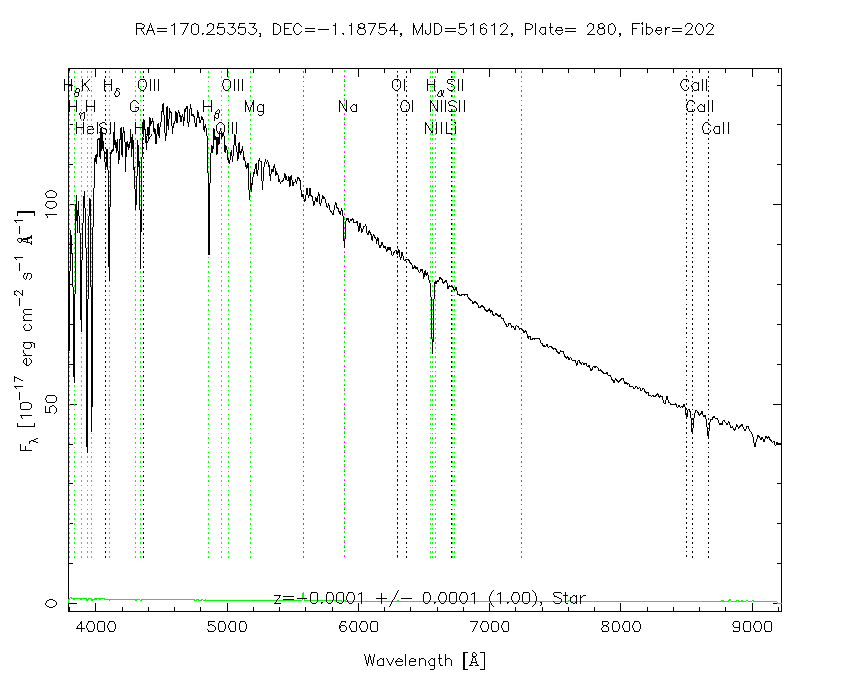
\includegraphics[width=0.7\textwidth]{Astrofysik/billeder/spektrum.png}
	\caption{Et typisk stjernespektrum. $y$-aksen skal forstås som intensitet, mens der
		på $x$-aksen er bølgelængde i Ångstrøm (\si{\angstrom}) (\SI{1}{\angstrom} = \SI{1e-10}{\metre}). Dykkene i intensitet
		er angivet med en overgang tilhørende et grundstof, som er identificeret i stjernens
		atmosfære.}
	\label{spektrum}
\end{figure}

I kapitlet Kvantemekanik blev tanken om kvantiserede energiniveauer introduceret, og denne teori videreføres i kapitlet Atom- og Molekylefysik til atomer. Eksempelvis er et hydrogenatom i et laboratorium på Jorden og et hydrogenatom i en stjerne langt væk i sidste ende samme grundstof, hvilket betyder at de opfører sig ens, hvis de er udsat for samme betingelser. Det betyder, at man kan bruge sin viden om grundstofferne her på Jorden til at få viden om f.eks. stjerner i universet. \\
Lidt oversimplificeret kan det siges, at stjerner er så varme og tætte i kernen, at atomkerner har energi nok til at kunne overkomme deres indbyrdes elektriske frastødning.\footnote{Dette ville ikke være muligt, hvis det ikke var for kvantetunnelering. Kvantetunnelering er kort sagt, at partikler kan passere gennem en energibarriere for at komme hen til et område med lav potentiel energi. Dette svarer til at en bold kan komme forbi en meget stor bakke, som den egentlig ikke har nok energi til, for at komme hen på den anden side af bakken, hvor der er en dyb dal bolden gerne vil ned i. Dette kan jo ikke lade sig gøre for en bold, men det er essentielt set det der sker inde i stjerner hele tiden.} Når atomkernerne kolliderer, fusionerer de til en tungere kerne, hvilket frigiver energi. Dette kan lade sig gøre, fordi den specielle relativitetsteori siger, at masse og energi i virkeligheden er to sider af samme sag; $E=mc^2$. Denne energi kan danne lys, som passerer ud gennem stjernen, men det sker ikke uhindret. Der er langt fra stjernens centrum til dens overflade, og lys og atomer påvirker hinanden. Bliver et atom ramt af en foton med lige præcis nok energi til at excitere en elektron fra en tilstand til en anden, vil denne elektron skifte energiniveau. På et senere tidspunkt henfalder elektronen til en lavere energitilstand under udsendelse af den overskydende energi i form af en foton. Denne fotons energi er netop karakteristisk for overgangen mellem de to omtalte energiniveauer. I en stjerne er der mange atomer udenfor kernen, så når fotonerne skal igennem det, vil rigtig mange af de mulige excitationer ske. Så når lyset passerer igennem vil de bølgelængder der lige passer med energiforskellene absorberes, og derfor kan vi se de mangler, når vi kigger på stjernen. Ved at sammenligne med kendte energiforskelle fra forskellige grundstoffer og kemiske forbindelser i laboratoriet, kan vi bestemme hvilke stoffer, der har påvirket et spektrum, og hvor meget af hver.  \\

En fotons energi kan af ligning \eqref{kvant:fotonEnergi} udtrykkes som $E=hc/\lambda$, hvor $\lambda$ er fotonens bølgelængde, $h$ er Plancks konstant, og $c$ er lysets fart. Fordi energiforskellene mellem elektronbaner i et atom er helt specifikke, er de tilhørende bølgelængder det også. Da vi kender grundstofferne godt, ved vi hvilke energiniveauforskelle, der er karakteristiske for hvert atom, så vi også kan finde dem i spektret fra en stjerne. Når vi kan genkende energiforskellene fra et bestemt grundstof, kan vi dermed finde ud af hvad stjernens overflade består af, se figur \ref{spektrum}. Kigger man grundigt på denne figur ser man, at hver absorptionslinje, hvilket man kalder dykkene, har en udbredelse - de har ikke kun én bestemt bølgelængde. Dette skyldes en kombination af mange ting, hvoraf to af dem er Dopplerforskydningen og Heisenbergs usikkerhedsrelation\footnote{Den mest kendte af disse er relationen mellem sted og impuls, men der eksisterer en tilsvarende tid og energi.}
\begin{align}
    \sigma_E^2\sigma_t^2 \geq \frac{\hbar}{2}
\end{align}
Pga. usikkerhedsrelationen har energien en usikkerhed, så den ikke nødvendigvis er, præcis hvad vi ellers forventer. Derudover står atomer ikke stille i stjernen, men bevæger sig i alle mulige retninger, med vidt forskellige hastigheder og energier.\footnote{Partikler i en gas følger approksimativt Maxwell-Boltzmannfordelingen, hvilket den interesserede læser kan finde andet materiale om.} Effekten af dette er, at atomerne er i bevægelse, når de udsender fotonen, der senere observeres på Jorden, og Dopplereffekten er netop en forskydning af bølgelængderne, som følge af at kilden bevæger sig. Det at atomerne bevæger sig i alle mulige retninger, gør at Dopplerforskydningen trækker i alle mulige retninger, hvilket resulterer i en udbredning af linjen frem for et skift i dens placering. Jo varmere en gas er, desto hurtigere bevæger gassens atomer sig. Det vil sige at absorptionslinjerne fra en varm stjerne er bredere end dem fra en kold stjerne. Yderligere har stjernens temperatur også indflydelse på dens grundstofsammensætning, da nogle stjerner kan være så varme, at bestemte grundstoffer ikke er stabile. I forhold til exoplaneter er stjernens sammensætning blandt andet interessant, fordi den påvirker sandsynligheden for forskellige typer af planeter. 
\section{Detektionsmetoder}
Der er mange måder at detektere exoplaneter på, men fælles for dem alle er, at de involverer lys fra enten planeten selv eller en anden lyskilde. At opdage planeter kræver derfor en forståelse af lys, hvordan det opstår og påvirkes af sine omgivelser. Det er dog muligt at få en god forståelse af de fysiske fænomener, der ligger til grund for disse metoder, uden en dybdegående forståelse af de teorier, der detaljeret beskriver fænomenerne. Eksempelvis kan gravitationslinsemetoden, som beskrevet senere, sagtens forstås overfladisk uden kendskab til generel relativitetsteori, hvis man er villig til at acceptere, at lys er påvirket af tyngdekraften analogt til objekter med masse. Formålet med dette afsnit er derfor at give en fænomenologisk og forhåbentlig intuitiv forståelse af, hvordan vi mennesker på Jorden kan opdage planeter uden for Solsystemet.\footnote{Til dette formål kan der med fordel henvises til nogle særdeles glimerende animationer på \url{https://exoplanets.nasa.gov/5-ways-to-find-a-planet/}.}

\subsection*{Direkte observation}

Den mest nærliggende metode er nok at pege sit teleskop mod et stjernesystem, og direkte se om noget ligner en planet. Dette er dog svært i praksis. Problemet er at exoplaneter fylder meget lidt på himlen, når de er så langt væk, så den eneste måde vi ville kunne se dem, var hvis de lyste. Men det er faktisk muligt. For hvis vi kigger i den infrarøde del af spektret, så lyser Solen fx kun 100 gange mere end Jupiter. %For når en stjerne lyser på en planet, kan planeten reflektere en del af lyset, og på den måde kan vi se den. 
Men hvilke planeter er så lettest at se? \\
Svaret er, at jo større en planet er, des mere lys vil den udsende. Derfor er planeterne detekteret ved direkte observation så store, at de er på grænsen til at være brune dværgstjerner. %reflekterer mere lys jo tættere den er på stjernen (der er mere lys at reflektere) og jo større den er (større planetoverflade til at reflektere lyset). Man kunne måske tænke planetens farve også har noget at sige, men denne effekt er meget mindre. %citation needed
%
%Indsæt formel
%
Lysstyrken bliver dog aldrig særlig høj sammenlignet med stjerner. Dette betyder, at metoden kun virker for gaskæmper, der kredser meget langt fra deres stjerner. Store planeter lyser mere, og afstanden gør at lyset kan skelnes fra stjernens. Vi kan kun se dem der kredser om stjerner tæt på vores eget solsystem, så fluxen ikke er faldet for meget med afstanden, for ligesom alt andet lys, aftager fluxen her som $F\propto D^{-2}$ ifølge afstandskvadratloven i ligning \eqref{afstandskv}. %varme jupita? Jupitorer?
%
Et eksempel på planeter opdaget ved direkte observation, er dem om stjernen HR 8799 på figur \ref{DI}. Her har man blokeret selve stjernens lys, så det ikke blænder for den smule infrarødt lys, vi modtager fra planeterne omkring den.

\begin{figure}[h!]
    \centering
    \begin{subfigure}{.45\textwidth}
        \centering
        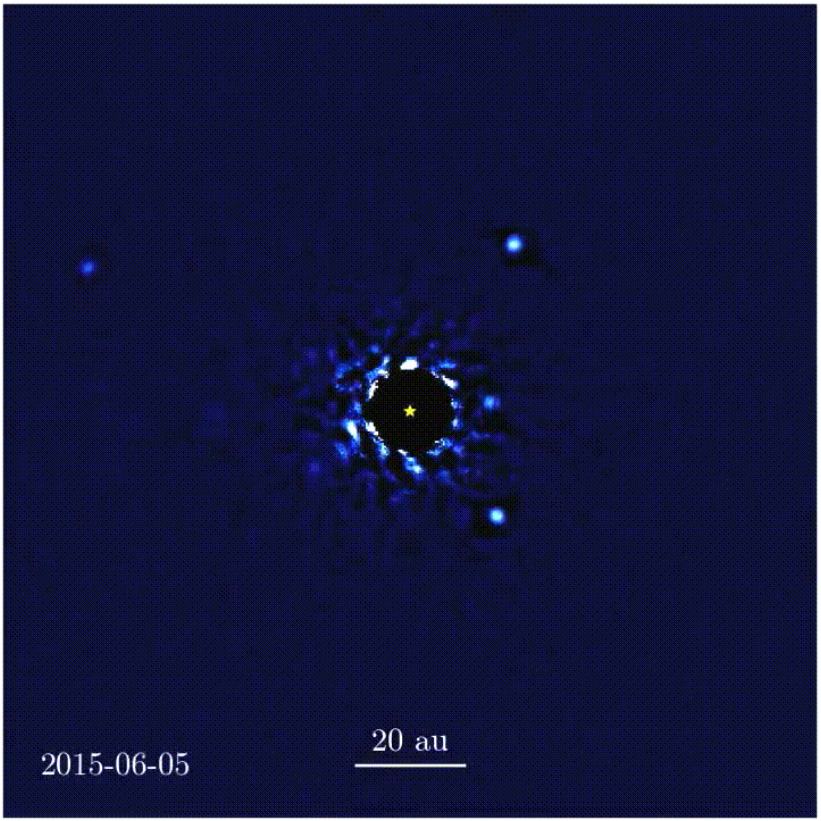
\includegraphics[width = 0.95\textwidth]{Astrofysik/billeder/Direct_imaging_image.PNG} 
        \caption{Direkte observation af mindst 4 store exoplaneter om stjernen HR 8799. AU står for astronomical unit og er afstanden fra Jorden til Solen. Til sammenligning er Jupiter 5 AU fra Solen.}
        \label{DI}
    \end{subfigure}
    \hspace{5mm}
    \begin{subfigure}{.45\textwidth}
        \centering
        \vspace{2mm}
        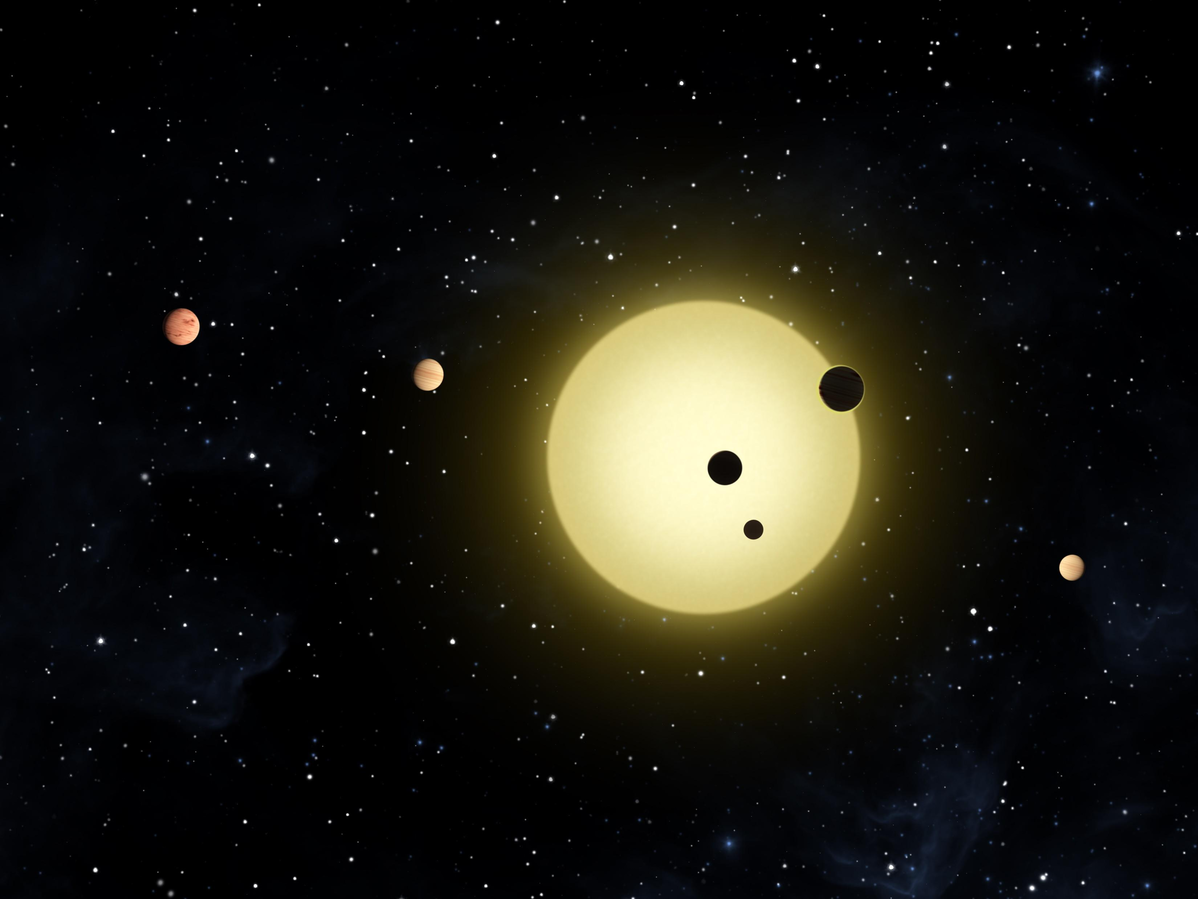
\includegraphics[width = 0.95\textwidth]{Astrofysik/billeder/Kepler11.png}
        \vspace{6mm}
        \caption{Kunstnerisk afbildning af stjernen Kepler 11 med planeter i transit.}
        \label{Kepler11}
    \end{subfigure}
    \caption{Til venstre ses en direkte observation af exoplaneter og til højre en illustration af transitmetoden, hvor planeter skygger for stjernen.}
\end{figure}

\subsection*{Transitmetoden}
%https://www.paulanthonywilson.com/exoplanets/exoplanet-detection-techniques/the-exoplanet-transit-method/

Den metode, vi har fundet flest exoplaneter med, er transitmetoden. Essensen af metoden er, at når en planet passerer ind foran en stjerne, som i den kunstneriske fortolkning på figur \ref{Kepler11}, så falder stjernens lysstyrke. Der sker en lille formørkelse, ligesom det bliver mørkt på Jorden, når Månen formørker Solen. Forskellen er, at vi er så langt væk fra disse planeter, at de modsat Månen ikke kan dække hele stjernen - uanset hvad størrelse planeten har (så længe den er mindre end stjernen). Det ses af figur \ref{UbetydeligRadius}. Noget der er tæt på kan skygge for en stor del af himlen, mens noget langt væk skal være større for at skygge for den samme vinkel. Alle andre stjerner end Solen er ca. uendeligt langt væk (mindst 4 lysår), så lyset fra hver ende af stjernen rammer os stort set parallelt. Deres planeter er også ca. uendeligt langt fra os, og derfor skal planeten være (næsten) på størrelsen med stjernen, hvis man skulle få en total formørkelse.
\begin{figure}[h!]
    \centering
    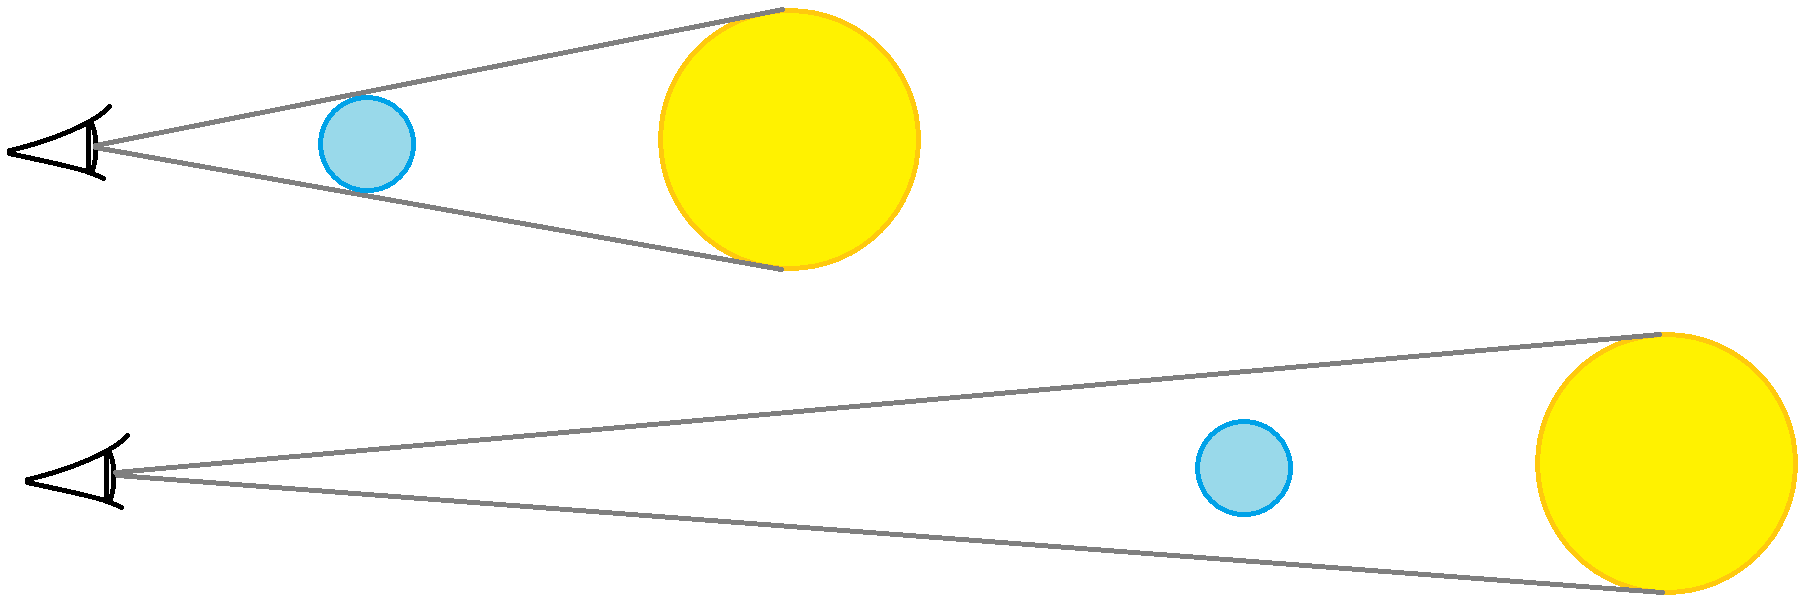
\includegraphics[width = 0.8\textwidth]{Astrofysik/billeder/UbetydeligRadius.png} 
    \caption{Illustration af at jo længere man er fra stjernen, des mindre afgørende er exoplanetens afstand til sin stjerne for hvor meget af lyset den dækker}
    \label{UbetydeligRadius} %misvisende navn
\end{figure}

Dette medfører også at planetens afstand til sin stjerne faktisk ikke har betydning for, hvor stor en formørkelse vi ser. Hvis lyset fra alle dele af stjernen flyver parallelt for at ramme os, så handler det kun om, hvor stor radius planeten har i forhold til stjernen. Antaget at lyset fra planeten er tæt på 0, er dybden af passagen

%Indsæt formlen med radier
\begin{align} \label{eq:DeltaL}
    \frac{\Delta L}{L_\star } = \left( \frac{R_p}{R_\star } \right)^2
    %F_{total} = F_\star  + F_p = \frac{I_\star }{}
\end{align}

Luminositeten af stjernen $L_\star $ kan vi nemt finde, da den hænger sammen med hvordan dens spektrum ser ud. $\Delta L$ er hvor meget lysstyrken falder under et transit, $R_p$ er planetens radius og $R_\star$ er stjernens radius. Så hvis vi kender stjernens egenskaber og måler dybdet af transittet, er planetens radius den eneste ubekendte, som vi derfor kan isolere i ligningen og beregne.
%
Metoden er selvfølgelig begrænset af, at stjernesystemet skal have en vinkel i forhold til os, hvor planetens bane krydser stjernen. Planeter der ikke opfylder dette, må vi detektere med andre metoder.
%
Fra Jorden kan vi måle fluxen fra en stjerne, så ved at gøre dette over tid, kan vi se om der er variationer, som indikerer tilstedeværelsen af en eller flere planeter. Man plotter en lyskurve med flux eller luminositet (ved at korrigere fluxen for afstanden) som funktion af tid, og ser efter mønstre i dette, som på figur \ref{transit}.
%
\begin{figure}
    \centering
    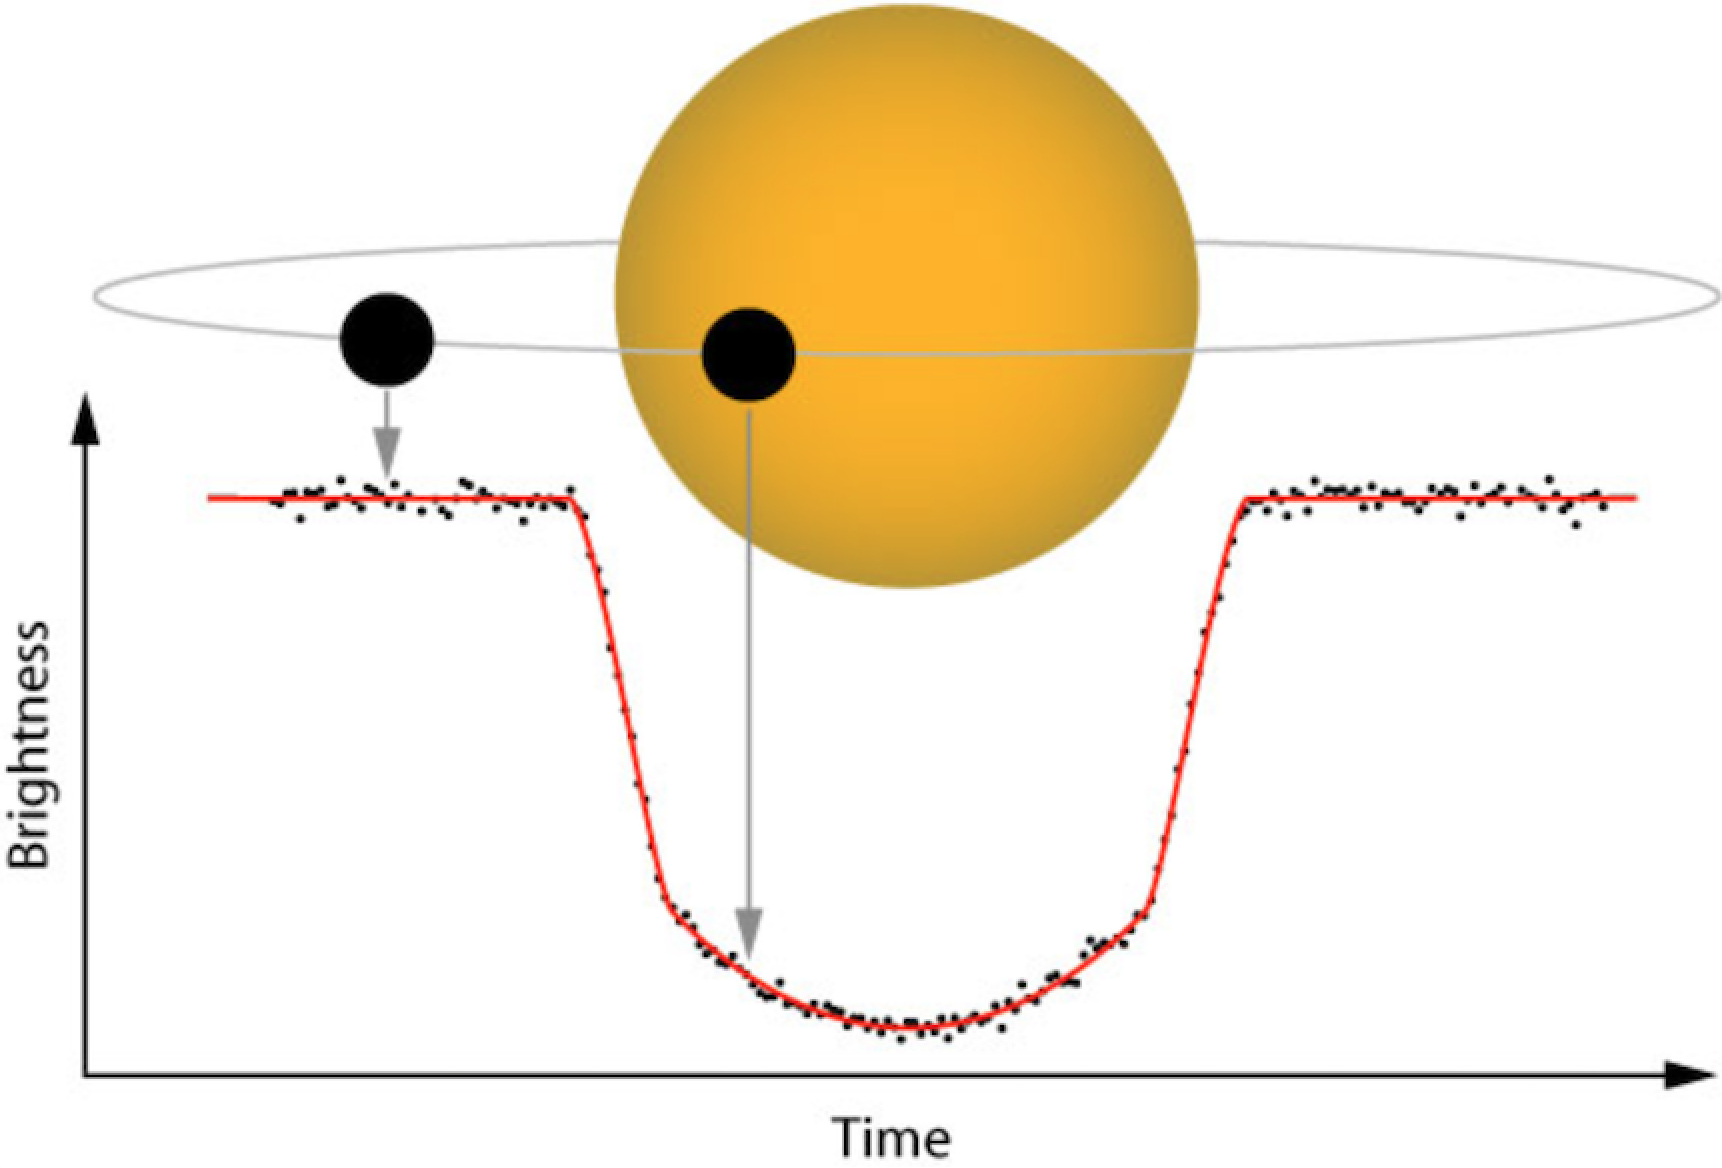
\includegraphics[width = 0.5\textwidth]{Astrofysik/billeder/transit.png}  
    \caption{Som planeten bevæger sig ind foran stjernen, skærmer den for mere af dens lys. På grafen vises luminositet som funktion af tid.}
    \label{transit}
\end{figure}
%
Når planeten først passerer ind over stjernen, ser vi et stejlt fald i lyskurven. Hældningen afhænger af planetens radius, da det for en stor planet vil tage længere tid før hele planeten er inde over stjernen. 
%
Derefter får vi en buet form i bunden af lyskurven, fordi stjernen lyser kraftigere i midten end ude i siden. Når planeten dækker stjernens midte, dækker den derfor en større andel af stjernens totale lys, end den ville, hvis den var ude i kanten af stjernen.
Når planeten passerer væk fra stjernen igen, ser vi det modsatte mønster. \\

Det er dog ikke det eneste interessante tidsrum. Når planeten ikke er ved at formørke stjernen, vil den nemlig stadig sende noget af dens lys i retning mod Jorden, og dermed øge lysstyrken. %\footnote{Planten reflekterer og udsender selvfølgelig hele tiden lys, men spørgsmålet er bare om det kan ses på Jorden. Hvis planeten er imellem dens stjerne og Jorden, vil planeten reflektere lys tilbage imod stjernen og altså væk fra Jorden.} 
Dette sker langsomt mens planeten bevæger sig om mod bagsiden af stjernen, hvor mere af mere af dens lys vil reflekteres - ligesom Månens faser ændrer sig som man nærmer sig fuldmåne. Men når planeten er direkte bag stjernen, får vi en planetformørkelse, hvor stjernen blokerer for lyset fra planeten, så der falder lyskurven til det niveau, der kun er genereret af stjernen selv. Dette kaldes det sekundære transit.
%
På figur \ref{fuld_lyskurve} ses en fuld lyskurve. Tidsaksen er elliptisk, så den følger hvordan planeten bevæger sig set fra Jorden. De stiplede linjer viser, hvordan fluxen ville være, hvis planeten og stjernen ikke påvirkede hinanden, mens den solide linje angiver den reelle lyskurve. Bemærk at selv natsiden af planeten vil bidrage med en smule lys. %Det kan fx skyldes refleksioner i atmosfæren og lys fra planeten selv.

\begin{figure}[h!]
    \centering
    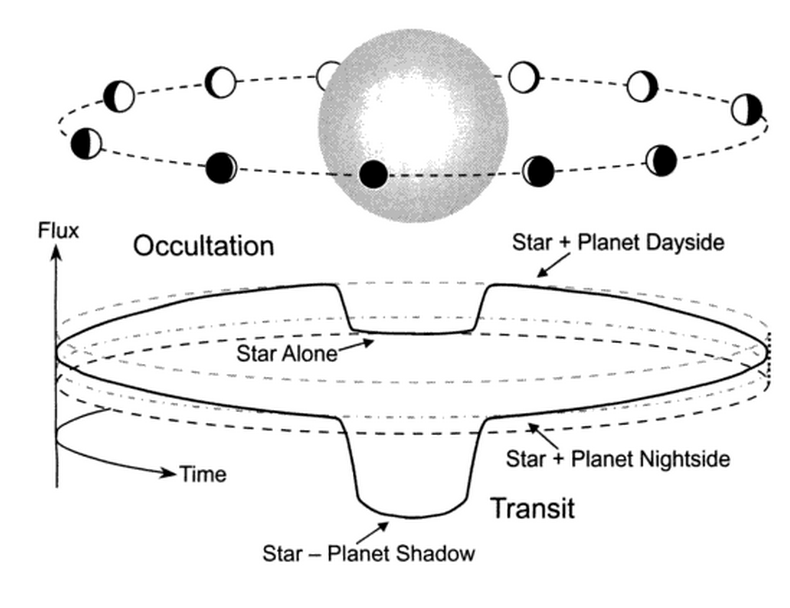
\includegraphics[width = 0.8\textwidth]{Astrofysik/billeder/fuld_lyskurve.png}  
    \caption{Lyskurven for et helt kredsløb med både primært og sekundært transit. Bemærk at tidensaksen er elliptisk, og fluxen er konstant hvis man holder en konstant højde over tidsaksen. \emph{Kilde: Aldaron, https://commons.wikimedia.org/w/index.php?curid=7274700}}
    \label{fuld_lyskurve}
\end{figure}

Ud fra transitmetoden kan man få mange oplysninger om planeten og dens stjernesystem:
\begin{itemize}
    \item \textbf{Planetens radius} kan fås fra hvor stor en del af stjernens lys der dækkes, men hænger også sammen med hældningen på lyskurven mens hele planetens overflade ikke dækker stjernen. Beregnet fra transittets dybde i enheder af stjernens luminositet $\frac{\Delta L}{L_\star }$ får man
    \begin{align}
        R_p = R_\star  \sqrt{\frac{\Delta L}{L_\star }}
    \end{align}
    \item \textbf{Inklinationsvinklen}, som er planetbanens hældning i forhold til os, kan vi også finde. Hvis planeten passerer ude i kanten af stjernen vil passagen nemlig tage kortere tid og lyskurvens form ændres.
    \item \textbf{Perioden} (dvs. årets længde for planeten) samt planetens \textbf{afstand} til stjernen hænger sammen ifølge Keplers 3. lov, hvis man kan estimere massen af systemet. De kan bestemmes ved at vente og se, hvornår dykket i lysstyrken vender tilbage, som følge af at planeten har været hele vejen rundt. Det øger desuden sikkerheden af, at vi virkelig har fundet en planet, jo flere gange signalet vender tilbage, da dyk i intensitet kan skyldes mange andre ting også. % + mange andre ting. "impact parameter", or how close to the center of the star the planet transits, the size of the star (or more precisely, how dense the star is), and the eccentricity of the planet's orbit, or how close to a circle the planet's orbit is"
    \item \textbf{Temperaturen} af planeten kan fås gennem det sekundære transit. Når planeten er i sekundært transit, måler vi kun stjernens lys og kan finde dens spektrum. Når planeten så er lige ved siden af stjernen og reflekterer mest muligt, kan vi tage et spektrum, som vil være summen af spektret fra planeten og det fra stjernen. Ved så at trække stjernens spektrum fra, får vi planetens spektrum. Hvor meget lys vi får fra den, kan afsløre dens temperatur.
    \item \textbf{Atmosfæresammensætningen} er rigtig interessant, hvis vi vil vide om der er liv på planeten, da fx oxygen er en god biomarkør. Den kan vi både se gennem planetens spektrum fra det sekundære transit, og gennem hvordan noget af stjernens lys kan blive absorberet under det primære transit. Her vil en del af det nemlig passere igennem atmosfæren. Dette uddybes i afsnit \ref{sec:liv}.
    \item \textbf{Solpletter} på stjernen kan også måles. Hvis planeten passerer henover en solplet, vil den kortvarigt skærme for en mindre del af stjernens lys, så der kommer et bump opad på lyskurven.
    \item \textbf{Planetens rotation} i forhold til stjernen kan bestemmes ved at se på, hvornår hvilke dele af spektret blokeres. Dette vil vi ikke komme nærmere ind på her, men det kaldes Rossiter-McLaughlin-effekten og viser overraskende at, op til 25 \% af planeter af typen "Hot Jupitors" drejer modsat deres stjerne. 
    \end{itemize}
    
Endvidere kan man opdage ekstra planeter indirekte, hvis man ser at transitplaneterne opfører sig, som om en ekstra planet hiver i dem. Vi kan altså opnå utrolig meget viden ud fra det lys, vi modtager fra et stjernesystem, og vi ser, at karakteriseringen af exoplaneter er meget afhængigt af vores forståelse af stjerner.

\subsection*{Radialhastighedsmetoden}
Radialhastighedsmetoden er en anden effektiv metode. Radialhastighed er den del af en hastighedsvektor der peger mod observatøren, også kaldet den radielle komponent, som illustreret på figur \ref{radvel}. Det er derfor et mål for, hvor meget noget bevæger i vores retning. Hvor hurtigt det kommer tættere på eller længere væk fra os, selv hvis det i virkeligheden ikke bevæger sig direkte mod os. Grunden til at vi bruger radialhastigheden er, at den er nem at måle, og fra den kan man opnå information om:

\begin{figure}[h!]
    \centering
    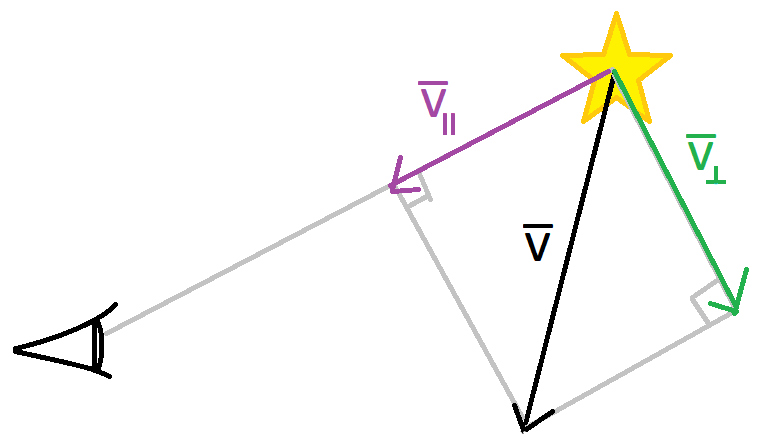
\includegraphics[width = 0.6\textwidth]{Astrofysik/billeder/radvel.png}  
    \caption{Illustration af en stjernes hastighed i forhold til en observatør. Den sorte pil angiver den totale hastighed, den grønne er den tangentielle hastighed, og den lilla er den radielle hastighed.}
    \label{radvel}
\end{figure}

\begin{itemize}
    %\item \textbf{Kraften} mellem stjernen og planeten fra Dopplerskiftet. %, hvilket er navnet på det fænomen at bølgers egenskaber påvirkes at kildens bevægelse. Dette er grunden til at lyden af et udrykningskøretøj ændres når det bevæger sig forbi en i trafikken.  %how % Dette har vi nu skrevet tidligere.
    \item \textbf{Perioden} hænger sammen med hvor ofte Dopplerforskydningen svinger mellem rødforskydning og blåforskydning. %Og perioden kan give os \textbf{afstanden} til stjernen gennem Keplers 3. lov.
    \item \textbf{Den radielle hastighed} af stjernen og planeten i deres fælles kredsløb kan godt findes, men den totale hastighed kræver andre metoder.
    \item \textbf{Massen} kan bestemmes, hvis vi kender stjernens masse, periode og radielle hastighed.
    %afstanden $r$ mellem stjernen og planeten og stjernens masse $M_\star$. $r$ og masserne $M_p$ og $M_\star$ hænger nemlig sammen ifølge Newtons tyngdelov. 
    Det er dog $M_p \sin(i)$ man finder, så uden at kende inklinationsvinklen $i$ har man kun en nedre grænse, da $\sin(i)$ kan være mellem 0 og 1. Men det plejer at passe inden for en faktor 2.  
    %\begin{align} \label{eq:FgNewton}
    %    F_g = G \frac{M_\star M_p}{r^2}
    %\end{align}
    \item \textbf{Densitet} kan man beregne ud fra massen og radius ved $\rho = \frac{M}{4/3 \pi R^3}$, hvis vi også kender radius fra at have observeret planeten med transitmetoden. Denne densitet er et gennemsnit over hele planeten, der her er antaget sfærisk.
    \item \textbf{Materialet} kan bestemmes fra densiteten. Dette gøres meget groft, men nogle materialer sætter øvre og nedre grænser på densiteten, og vi kan sammenligne med kendte planeter med lignende densiteter.
\end{itemize}

Radialhastighedsmetoden udnytter at planeten har masse, hvorfor både stjernen og planeten bevæger sig om et fælles massemidtpunkt. Eftersom stjernen er meget tungere end planeten, vil det resultere i at planeten bevæger sig meget mere end stjernen, og massemidtpunktet kan befinde sig inde i stjernen. Dette kan ses ud fra vægtstangsprincippet
\begin{align} \label{vstang}
    M_pr_p = M_\star r_\star 
\end{align}
hvor $M_p$ og $r_p$ er hhv. planetens masse og afstand til stjernen og planetens fælles massemidtpunkt, og ligeså for stjernen. For kontekstens skyld kan vores Solsystem nogenlunde approksimeres til kun at bestå af Solen og Jupiter, hvorfor afstanden fra Solens centrum til solsystemets massemidtpunkt, i solradier, er
\begin{align}
    r_\odot = \frac{M_\textit{\textsc{j}}r_\textit{\textsc{j}}}{M_\odot} = \SI{1.07}{R_\odot} \, ,
\end{align}
hvor subscriptet $\odot$ indikerer, at det er en af Solens egenskaber.\footnote{Jorden kan tilsvarende angives ved subscriptet $\oplus$.} Det ses altså, at Solen roterer om et punkt lidt uden for dens overflade, og det kan derfor konkluderes at Solen bevæger sig, men ikke ret meget ift. planeterne omkring den.\\

Stjernens bevægelse kan dog være nok til, at det kan ses fra Jorden. Vi har svært ved at observere stjernens bevægelse i andre retninger en den radielle, så stjernen ser ud som om den svinger skiftevis mod os og væk fra os. Lys er elektromagnetiske bølger og påvirkes derfor af Dopplerforskydning som beskrevet i sektion \ref{exointro}.
%lidt groft sagt kan det siges at når stjernen bevæger sig mod os, så skubber den bølgen sammen, hvorved bølgelængden bliver kortere og modsat når den bevæger sig væk fra os. Denne forskydning af bølgelængde som følge af kildens hastighed kaldes en Dopplerforskydning eller rød-/blåforskydning i astronomi, hvor farven angiver retningen.
%Da rød svarer til lange bølgelængder og blå til korte (indenfor det synlige spektrum), så refererer rødforskydning til noget som bevæger sig væk fra os og vice versa. Dette virker fordi en lyskildes spektrum afhænger meget distinkt af hvor lyset kommer fra og hvad det har skulle bevæge sig igennem for at nå til jorden. Stjerners overflader består af forskellige grundstoffer og forskellen mellem to energiniveauer i hvert grundstof svarer til en hel bestemt bølgelængde. Da der er mange mulige overgange for hvert atom kan det identificeres ud fra de spektrallinjer, atomet skaber i spektret, altså hvilke bølgelængder, der absorberes af atomet. 
Dopplereffekten gør det at hele spektret flyttes, og det betyder, at stjernes hastighed kan bestemmes ved at finde ud af, hvor meget spektret skal "flyttes" for at spektrallinjerne falder tilbage til den form det ville have, hvis det ikke var blevet Dopplerforskudt.

\begin{figure}[h!]
    \centering
    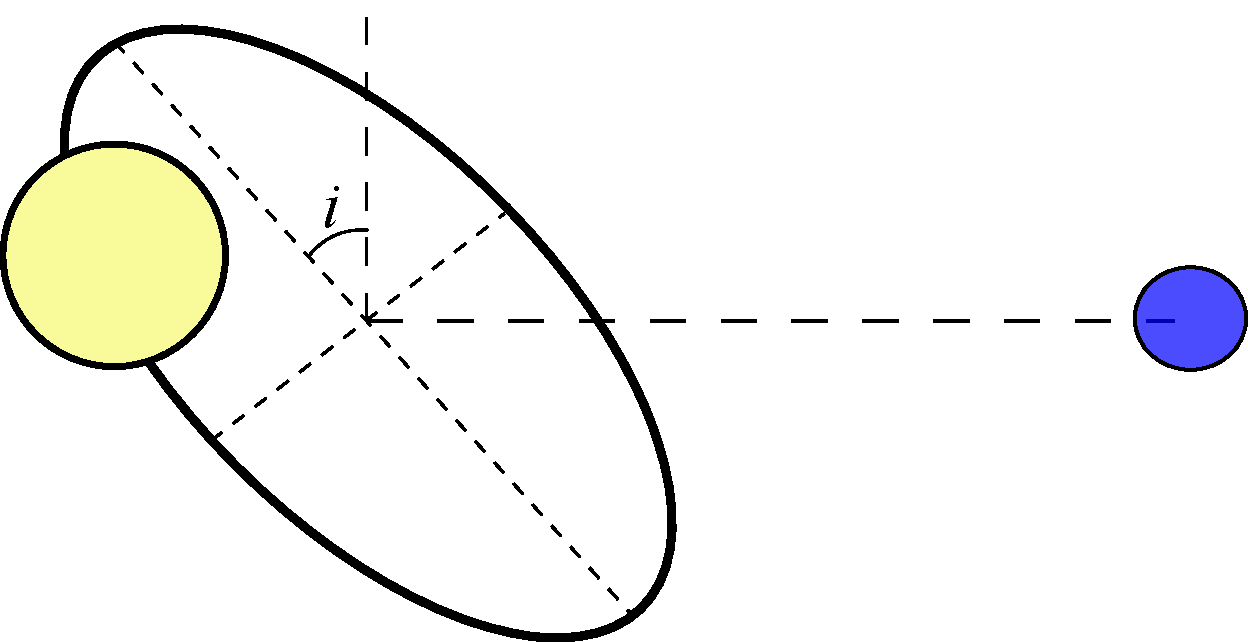
\includegraphics[width=.7\textwidth]{Astrofysik/billeder/Inklinitionsvinkel.pdf}
    \caption{Stærkt fortegnet illustration af situationen for radialhastighedsmetoden. Den hastighed vi kan bestemme på Jorden ud fra Dopplerforskydningen er en radielle bevægelse i samme plan som vi ser stjernen, dvs. langs med den stiplede linje fra Jorden. Stjernen kan dog også bevæge sig i de to andre dimensioner, som ikke kan "ses" fra Jorden. Den samlede fart afhænger derfor af inklinationsvinklen $i$, som er vinklen mellem den plan stjernen bevæger sig i og synslinjen til stjernen fra Jorden.} %Og en faktor mere, right? Det kan jo være elliptisk
    \label{fig:vsini}
\end{figure}

\subsubsection{Estimat af planetens masse fra radialhastighedsmetoden}
Planetens masse og afstand til sin stjerne er helt essentielle parametre, så dem vil vi forsøge at bestemme med udgangspunkt i Keplers 3. lov for to-legemesystemets fælles bevægelse
\begin{align} \label{kepler3lov}
    \frac{P^2}{r^3} = \frac{4\pi^2}{G(M_p+M_\star )}
\end{align}
hvor $P$ er stjernen og planetens fælles periode, $G$ er Newtons gravitationskonstant, $r$ er afstanden mellem dem, og det kan også udtrykkes som summen af afstandenene fra hhv. stjernen og planeten til deres fælles massemidtpunkt. Antager vi nu, at både planeten og stjernen er i jævn cirkelbevægelse omkring deres fælles massemidtpunkt, kan vi anvende ligning \ref{vstang} og få
\begin{align}
    r = r_\star+r_p  = r_\star  + \frac{M_\star r_\star }{M_p}
\end{align}
Det er dog afstanden i tredje, der skal bruges til Keplers 3. lov, som så det opskriver vi
\begin{align} \label{rvstang}
    r^3 = r_\star ^3\left(1 + \frac{M_\star }{M_p}\right)^3 = r_\star ^3\left(\frac{M_\star  + M_p}{M_p}\right)^3
\end{align}
Antagelsen om jævn cirkelbevægelse er nødvendig for at opnå et simpelt udtryk for planetens masse, selvom den ikke altid er lige god, men dog tilstrækkelig til at få en idé om størrelsen.\footnote{Det er en generel ting i fysik at jo mere præcist vi forsøget at beskrive verden desto mere kompliceret bliver det, og at vi derfor hurtigt bliver nødt til at approksimere, hvilket specielt ses i kapitlerne om analytisk mekanik og atom- og molekylefysik.} \\
Perioden er den tid det tager et objekt at bevæge sig en hel omgang om sit rotationspunkt, hvilket også kan udtrykkes som forholdet mellem den tilbagelagte afstand og hastigheden. For stjernen bliver det derfor (antaget cirkelbevægelse)
\begin{align}
    P_\star  = \frac{2\pi r_\star }{v} \label{Pstar}
    %P_\star  = \frac{2\pi r_\star }{v_\star ^\mathrm{rad}} \label{Pstar}
\end{align}
hvor $v$ er stjernens samlede fart. Problemet er bare, at med Dopplerforskydning kan vi kun se farten parallelt med vores synslinje dvs. den radielle hastighed $v_{||}$. Hvis stjernen ikke roterer i samme plan som vi ser den fra, er der en hastighedskomponent vi ikke får målt, se figur \ref{fig:vsini}. Fra denne figur ses det, at vi vha. trigonometri kan udtrykke den observerede hastighed $v_{||}$ som

%hvor $||$ er et superscript, der indikerer at der er tale om en radiel hastighed parallel med vores synslinje. Radialhastighedsmetoden er jo netop, at vi kan bestemme den radielle fart, $v_{||}$, ud fra spektroskopi (at kigge på spektrallinjer). Problemet er bare, at stjernen ikke nødvendigvis roterer i det plan vi ser den fra, se figur \ref{fig:vsini}. Fra denne figur ses det, at vi kan udtrykke den observerede hastighed $v_{||}$ vha. trigonometri.
\begin{align}
    v_{||} = v \sin(i) \, ,
    %\tilde{v} = v_{*,\,\mathrm{obs}}^\mathrm{rad} = v_\star ^\mathrm{rad}\sin(i)
\end{align}
hvor $i$ er inklinationsvinklen og $v$ er stjernens samlede fart. Herfra skiftes notationen, som indikeret ved det første lighedstegn ovenfor, da det er simplere at skrive. %da det er til at blive idiot af symbolet $v_{*,\,\mathrm{obs}}^\mathrm{rad}$, selvom det fortæller præcist hvad det betyder. 
Herved bliver perioden
\begin{align}
    P_\star  = \frac{2\pi r_\star \sin(i)}{v_{||}} 
\end{align}
Kombineres dette med Keplers 3. lov, ligning \eqref{kepler3lov}, fås
\begin{align} \label{eq:K3Fancy}
    \frac{4\pi^2}{G(M_p+M_\star )} = \frac{P_\star ^2}{r ^3} = \frac{P_\star ^3}{P_\star r ^3} = P_\star ^3 (P_\star r ^3)^{-1} = \left(\frac{2\pi r_\star \sin(i)}{v_{||}}\right)^3\left(P_\star r^3\right)^{-1}
\end{align}
Tricket med at forlænge brøken med perioden kan virke uintuitivt, men det tillader os at benytte ligning \eqref{rvstang} således
\begin{equation} \label{eq:m_planet}
\begin{aligned}
    \frac{1}{G} &= 2\pi\sin^3(i)\left[v_{||}^3P_\star \dfrac{(M_\star +M_p)^2}{M_p^3}\right]^{-1} \\
    \implies M_p^3\sin^3i &= \frac{P_\star v_{||}^3(M_\star +M_p)^2}{2\pi G}
\end{aligned}
\end{equation}
Det virker som om der sker en hel masse her, men i virkeligheden er der ikke sket andet, end indsættelsen af ligning \eqref{rvstang} og en efterfølgende reduktion af ligningen til en nogenlunde pæn form. Dette opfordres læseren til at tjekke efter. \\
Stjernen vil ofte være meget tungere end planeten, hvorfor kan være en rimelig antagelse, at summen af de to masser bare er stjernens masse, $M_\star  + M_p\approx M_\star $, hvorved følgende opnås
\begin{align}
    M_p\sin(i) \approx v_{||}\left(\frac{P_\star M_\star ^2}{2\pi G}\right)^{1/3}
\end{align}
Da udtrykket afhænger af $i$, kræver dette, at $i$ kan bestemmes på andre måder. Det er en klar svaghed ved metoden, da $i$ kan være svær at bestemme. Men man får en nedre grænse for massen. Derudover er radialhastighedsmetoden selektiv over for tunge planeter på tæt stjernen, da $v_{||}$ må være stor nok til at vi kan se, hvordan den trækker i stjernen.

\subsection*{Astrometri}
Udfordringen ved radialhastighedsmetoden er, at vi netop kun måler den radielle komponent af hastigheden, og ikke kender den fulde version. For at metoden kan virke optimalt, skal $\sin(i)$ helst være så stor som muligt, da Dopplerforskydningen så er størst (og man får et størst muligt minimum for massen). Er $\sin(i)$ meget lille, svarer det til at se systemet enten oppefra eller nedefra. Så bliver Dopplerforskydningen relativt lille, og radialhastighedsmetoden bliver svær at bruge. Men planeten vil stadig hive i stjernen langs andre akser - vinkelret på vores synsfelt. Teknisk set kan denne bevægelse ses, og kan dette gøres konsistent nok, er det muligt at bruge det til at detektere planeten i bane om stjernen. Stjerner er dog så langt væk, at selvom de bevæger sig meget, så ser bevægelsen lille ud herfra, og det kræver meget store teleskoper med meget god opløsning. \\

Med astrometri kan vi opnå information om %observere parametre omkring stjernen og planetens indbyrdes bevægelse, hvorfor der kan opnås information om
\begin{itemize}
    \item \textbf{Inklinationsvinklen} af systemet.
    \item \textbf{Massen} kan bestemmes, lidt parallelt til hvordan det gøres for radialhastighedsmetoden.
    \item Kan inklinationsvinklen bestemmes, samtidig med at der er data, som kan bruges til radialhastighedsmetoden, bliver det muligt at bruge denne til at bestemme fx massen med høj præcision.
    \item I kombination med direkte observation af planeten kan planetens banebevægelse beskrives med høj præcision.
\end{itemize}

\begin{figure}[h!]
    \centering
    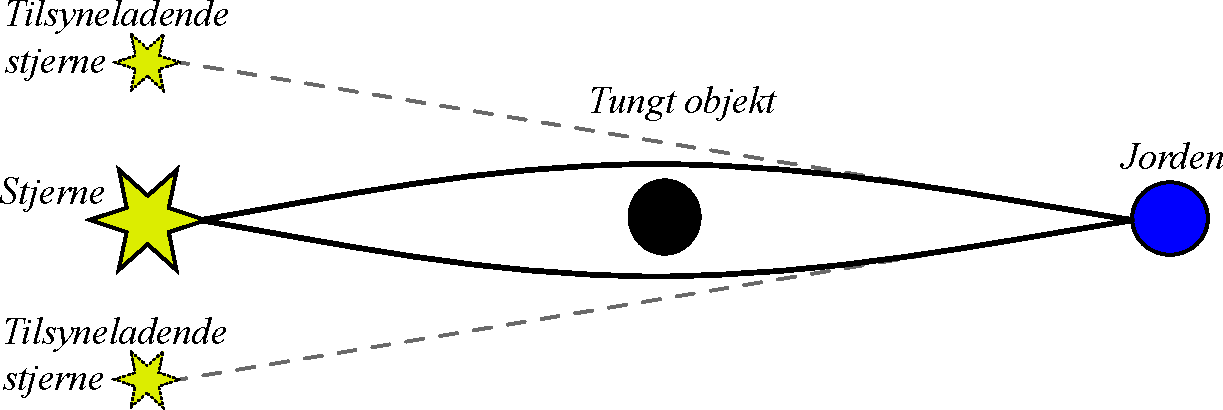
\includegraphics[width=\textwidth]{Astrofysik/billeder/GravLinse.pdf}
    \caption{Lys udsendt fra en fjerntliggende lyskilde afbøjes af tyngdefeltet fra objektet i midten. Som de grå stiplede linjer indikerer ser det ud til at der skulle være to mindre identiske stjerner, frem for én større, når de ses på Jorden.}
    \label{fig:GravLinse}
\end{figure}

%Liste med egenskaber man kan finde
\subsection*{Gravitationslinsemetoden} \label{sec:GravLinse}
Klassisk set er lys masseløse elektromagnetiske bølger, der ikke påvirkes af tyngdekraften. Det falder dog ud af den specielle relativitetsteori, at energi og masse er to sider af samme sag, og da lys har energi, så påvirkes det også af tyngdekraften. Det bevæger sig stadig i lige linjer, men vil se bøjet ud, fordi tyngdekraften ændrer på, hvad en lige linje er - det får selve rummet til at krumme, som beskrevet i generel relativitetsteori. Denne effekt er dog lille nok til, at den klassiske beskrivelse holder i mange situationer, hvorfor den klassiske beskrivelse ikke altid bør forkastes. Astrofysiske objekter kan dog være så tunge, at effekter af rumtidens krumning observeres. Dette ses blandt andet ved eksistensen af det, som kaldes \textit{gravitationelle linser}. En linse spreder eller fokuserer lys, hvilket uddybes i kapitel \ref{cha:Optik}. En gravitationel linse virker essentielt set på samme måde, som en almindelig konveks linse, da gravitation kun er tiltrækkende.\footnote{Dette gælder så længe negativ masse ikke er en ting, hvilket alt empiri peger mod.} I figur \ref{fig:GravLinse} ses en illustration af princippet i en gravitationel linse, hvor lyset fra den bagvedliggende kilde fokuseres omkring et tungt objekt. Det medfører at vi modtager mere lys, end hvis det midterste legeme ikke havde været der, og at lyskildens position på himlen bliver forskudt, forvrænget og måske splittet til flere versioner forskellige steder. Hvis objektet i midten bevæger sig, så ændres fluxen på Jorden sig markant. På denne måde kan tunge objekter, som ikke selv udsender nok lys, til at vi kan se dem, detekteres på Jorden. Hvis det midterste objekt er en stjerne med en tilhørende planet, vil der være et tidspunkt, hvor planetens position får fluxen fra den fjerne stjerne til i "kort"  tid at øges og falde igen. Så hvis man plotter fluxen på en lyskurve, vil det give et lille peak. Hvis dette peak kan karakteriseres ud fra flere målinger, og der er samme effekt alle stedet, så er det muligt at konkludere, at en ny planet er fundet. \\

Ud fra gravitationslinsemetoden, hvor det afbøjende objekt er et stjernesystem, kan man opnå information om
\begin{itemize}
    \item \textbf{Systemets masse} ved at se hvor forvrænget det bagvedliggende lys bliver. Hvis lyskilden danner en ring kan man fx måle dens størrelse. Man må tage højde for afstandene mellem lyskilden, stjernesystemet og Jorden, samt hvor langt objekterne er fra hinanden på himlen. Hvis lyskilden er næsten på samme synslinje fra Jorden som stjernesystemet, vil linseeffekten påvirke det mere.
    %\item \textbf{Einsteinringens størrelse} for stjernesystemet, der hænger sammen med systemets masse og de indbyrdes afstande mellem baggrundsstjernen, systemet der forårsager lensingen, og Jorden. Massen er dog den samlede masse, hvorfor den inkluderer både stjerne, planet og hvad der ellers skulle være i stjernesystemet.
    \item \textbf{Masseforholdet} mellem stjernen og planeten kan findes, ved at se hvor stor linseeffekten er, når planeten bidrager i forhold til når den ikke gør. Det medfører, at \textbf{planetens masse} kan bestemmes, forudsat at stjernens masse kan bestemmes på anden vis. Metoden er særligt interessant, fordi man med gravitationslinser kan se selv relativt små planeter på størrelse med Mars.
    \item \textbf{Afstanden} mellem baggrundskilden og stjernesystemet kan approksimeres, hvis området hvori de to objekter er, er relativt kendt. Har man en grov idé om, hvor de to befinder sig, kan man sammenligne deres relative bevægelse med, hvordan ting i de områder typisk bevæger sig, og på den måde komme frem til en indbyrdes afstand.
    %\item \textbf{Højsopløsningsdata} af exoplaneter, da man i dag har den teoretiske forståelse, til at benytte Solen som en gravitationel linse, der kan fokusere lys andre steder fra, og derved forbedre opløseligheden af målinger derfra. Man har endnu ikke den praktiske kunnen, men det er måske en mulighed i fremtiden. % Kilde: https://journals.aps.org/prd/abstract/10.1103/PhysRevD.96.024008#fulltext
    \item \textbf{Afstanden} fra planeten til stjernen kan ses, men kun ved et bestemt tidspunkt. %Perioden? Afstanden til stjernen?
\end{itemize}

Gravitationslinsemetoden er desuden speciel idet den tillader os at se planeter meget langt væk fra os selv - helt ind mod galaksens centrum.

En ulempe ved gravitationslinsemetoden er, at den den er afhængig af et objekt der passerer bagved stjernesystemet, og som sandsynligvis aldrig vender tilbage. Så man har kun kort tid til observationerne (timer til dage), og de kan ikke gentages.

Der kan desuden være en fremtid i at anvende Solen som gravitationel linse til at tage højopløsningdata fra fjerne objekter. Dette har vi dog ikke den praktiske kunnen til endnu.

% Kilde: http://spiff.rit.edu/classes/resceu/lectures/microlens/microlens.html

%\subsection*{Pulsartiming}


\begin{figure}[h!]
    \centering
    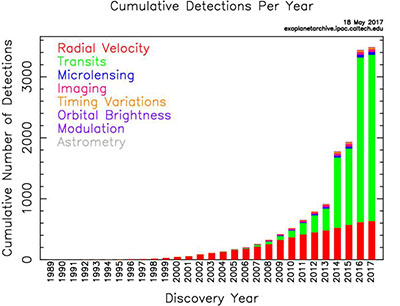
\includegraphics[width = 0.8\textwidth]{Astrofysik/billeder/AntalFundne.jpg}  
    \caption{Antal fundne exoplaneter efter årstal og sorteret efter metode. \textit{Kilde: NASA IPAC Exoplanet Science Institute}}
    \label{antal_fundne}
\end{figure}

\subsection*{Sammenligning}
Da der er så mange forskellige metoder at detektere exoplaneter med (også nogle vi ikke har nævnt), er det værdifuldt at have et overblik over deres styrker og svageheder. Af figur \ref{antal_fundne} ses, at vi generelt bliver bedre til at finde exoplaneter, hvilket der kan være mange årsager til. Den mest oplagte er at instrumenter, teknologier og vores viden om exoplaneter forbedres. Det handler langt hen af vejen om at se små ændringer i det lys en stjerne udsender, sammenlignet med hvordan det ellers ville have set ud. Jordens atmosfære kan både sprede lys, absorbere dele af det og udsende mere, hvorfor det giver mere præcise målinger at benytte rumteleskoper for at undgå disse forstyrrelser. Så når vi får flere af disse, og dedikerer mere af deres tid til exoplaneter, vil vi også gøre flere opdagelser i feltet. Der er fx høje forventninger til James Webb Space Telescope, som med sin høje præcision måske vil kunne afgøre, om der er liv på andre planeter.  %Som flere missioner bliver iværksat gøres mere data tilgængeligt for forskere, hvorfor der er flere mulige stjerner at kigge på. 
Erfaringen fra tidligere missioner kan også forbedre de næste. Derudover må nogen jo betale for forskningen, og når først der er publicerede artikler, der viser at noget er muligt, og at det kan være interessant at undersøge noget, så bliver det lettere at skaffe penge til. \\ %Det er derfor ikke urealistisk at antage, at mængden af tid og penge, der bruges på at finde exoplaneter, er stigende. \\

Det ses også at radialhastighedsmetoden var dominerende i starten, indtil den i 2014 blev overhalet af transitmetoden i antal opdagede planeter. %En mulig årsag til dette kan være at transitmetoden måske kræver en højere præcision i målingerne af stjernens lys.
Keplersatelitten blev sat i kredsløb om Jorden i 2009 og har siden 2011 sendt data tilbage om tusindvis af exoplaneter, primært fundet vha. transitmetoden. %til Jorden om det galaktiske nabolag. Keplers tilstedeværelse giver bedre data, der gør det muligt at detektere flere exoplaneter. Som rumteleskob bliver Keplersatelitten ikke påvirket af Jordens atmosfære, som teleskoper nede på jorden, hvilket kan være afgørende for opdagelsen af exoplaneter. \\

Nogle detektionsmetoder er meget afhængige af, hvordan stjernen og planetens bevægelse er orienteret, ift. det plan hvori vi ser dem. Selvom en planet kan være kæmpestor og meget tæt på sin stjerne, så den hiver meget i stjernen, kan den være stort set usynlig for radialhastighedsmetoden, hvis $i\approx\SI{0}{\degree}$ eller $i\approx\SI{90}{\degree}$. Stjernen vil rigtig nok bevæge sig en hel masse, men ikke parallelt med synslinjen, så lyset ikke Dopplerforskydes meget. Denne planet ville dog være ideel til at detektere med astrometri, men med henvisning til figur \ref{antal_fundne} ses det, at astrometri ikke er nær så effektiv som radialhastighedsmetoden, hvorfor planeten måske overses. \\

\begin{figure}[h!]
    \centering
    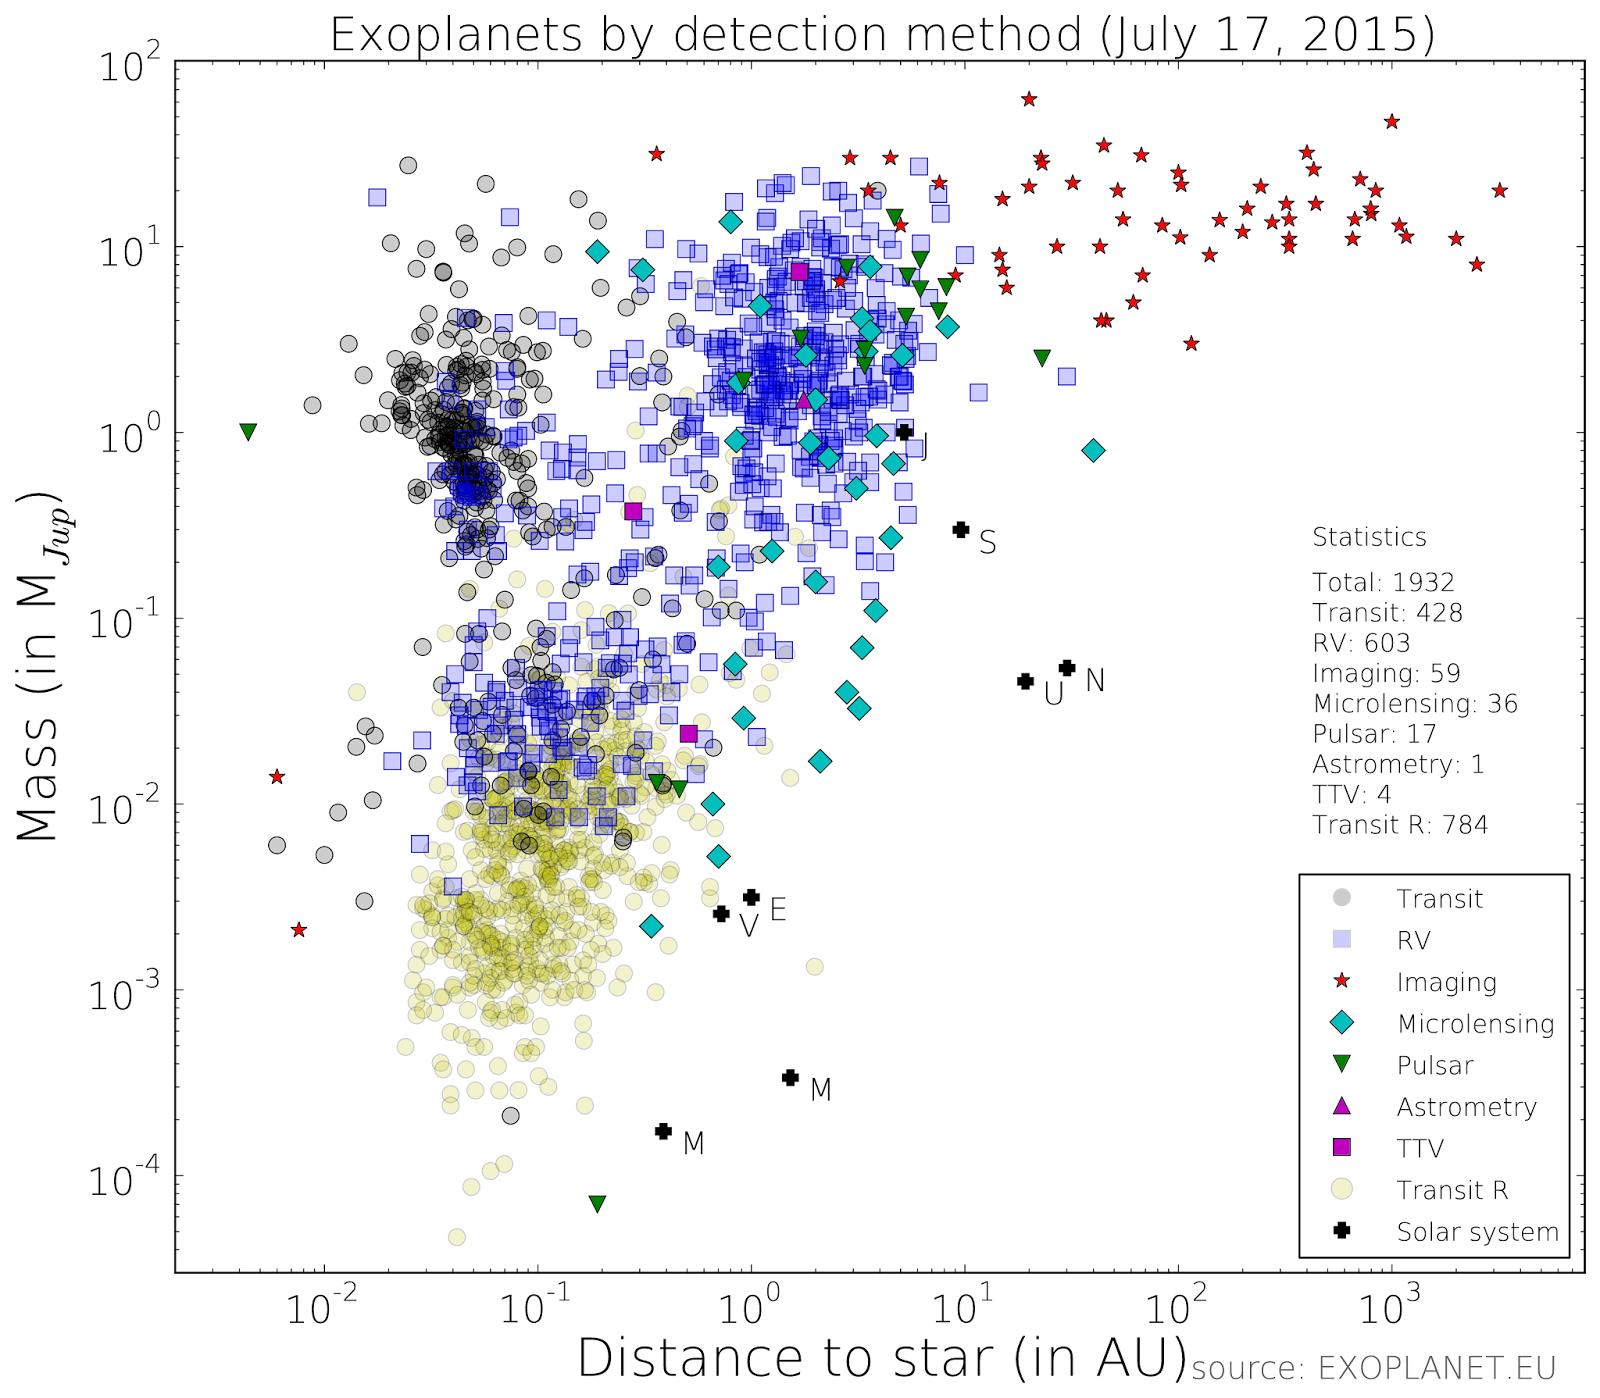
\includegraphics[width=.8\textwidth]{Astrofysik/billeder/sammenligning.PNG}
    \caption{Her ses de pr. 17. juli 2015 fundne exoplaneter, deres masse, afstand til den nærmeste stjerne, og den metode de er fundet ved. Yderligere er planeterne i Solsystemet indtegnet med sort. Det ses, at planeter meget langt fra deres stjerne kun er fundet ved direkte observation (dem fundet tæt på stjernen er formegentlig en fejl), samt at de andre metoder mest finder tunge planeter, tæt på deres stjerne. Bemærk de logaritmiske akser og enhederne - $M_{jup}$ er Jupitermasser og AU er Jordens afstand til Solen. \emph{Kilde: exoplanet-diagrams.blogspot.dk/2015/07/exoplanets-by-detection-method.html}}
    \label{fig:sammenligning}
\end{figure}

I afsnittet om transitmetoden fremgår det, at jo større planeten er relativt til stjernen, desto tydeligere vil den sænke systemets luminositet, se ligning \ref{eq:DeltaL}. Det betyder, at en "stor" planet i bane om en "lille" stjerne vil være lettere at detektere på denne måde end den modsatte situation. Dette er et eksempel på en relativt generel tendens i detektionsmetoderne. De fleste favoriserer store planeter tæt på deres stjerne, da de så påvirker stjernen mest. Det er vigtigt, da det ofte er stjernens lys, og ikke planetens, der ses på Jorden, og planeten detekteres ved den måde den får stjernen til at bevæge sig på. Dette kan ses fra Newtons tyngdelov,
\begin{align} \label{eq:FgNewton}
    F_g = G \frac{M_\star M_p}{r^2},
\end{align}
hvor kraften er proportional med planetens masse over dens kvadrerede afstand til stjernen. Denne effekt finder sted ligeså snart stjernens bevægelse benyttes, hvorfor det ikke er aktuelt for eksempelvis direkte observation, men som det fremgår af afsnittet favoriserer denne metode også store, tunge planeter, dog via nogle andre argumenter. \\

I figur \ref{fig:sammenligning} ses et plot over kendte exoplaneter, deres masse, afstand til nærmeste stjerne samt den metode vi har fundet dem med. Ovenfor blev det konkluderet at tunge planeter tæt på deres stjerne, er favoriseret af de fleste detektionsmetoder. Dette ses ved de mange punkter øverste venstre hjørne på figuren, sammenlignet med at nederste højre hjørne er fuldstændig tomt - men der er også en faktor fra, at der nok blot findes færre små planeter langt fra deres stjerner.  Det skal også nævnes at planeter markeret som "Transit R", adskiller sig udelukkende fra "Transit", ved at massen er et kvalificeret gæt. Man har brugt planetens radius, antaget en densitet der er rimelig for planeter af dens størrelse, og derved estimeret massen. Det ses også tydeligt at radialhastighedsmetoden og transitmetoden er de klart mest effektive, samt at transitmetoden har den mest markante favorisering af planeter, som er tæt på. For at noget kan kaldes en planet, er det ikke nok at observere ét transit, så transitmetoden kræver at årets længde på planeten er kort nok - men perioden hænger sammen med afstanden til stjernen ifølge  Keplers 3. lov, ligning \ref{kepler3lov}, så det sætter en begrænsning på afstanden. Radialhastighedsmetoden favoriserer hovedsageligt tunge planeter, som kan være lidt længere væk.  %Keplers 3. lov, ligning \ref{kepler3lov}, giver at perioden er stor, hvis også afstanden til stjernen er stor, hvilket betyder, at der går lang tid mellem transit, hvilket mindsker sandsynligheden for at observere det flere gange. \\
Det er også meget markant, hvordan direkte observationer skiller sig ud. Det er den eneste metode som har fundet de fjerne planeter, som i nogle tilfælde også ligger meget længere fra deres stjerne end Neptun gør fra Solen. De to små planeter, der er fundet med direkte observation, er der en risiko for at det er fejl,\footnote{\url{http://exoplanet-diagrams.blogspot.dk/2015/07/exoplanets-by-detection-method.html?m=1}} hvilket blot styrker konklusionen om, hvilke planeter direkte observation favoriserer. \\
Her er også plottet nogle planeter, der er fundet med metoder, der ikke er beskrevet her, men de er ikke essentielle for at forstå de generelle tendenser i plottet.

Det er ret markant som Solsystemets planeter stort set falder helt uden for den tendens, vi ser for fundne exoplaneter. Dette kan skyldes mange ting. En mulighed er, at Solsystemet er meget specielt, hvilket kunne reducere sandsynligheden for liv andre steder - for hvad nu hvis liv kræver specielle forhold, siden vi netop er i et usandsynligt system? En anden mulighed er, at Solsystemet bare er et af mange stjernesystemer, og at der intet specielt er ved det, men at vi ikke er i stand til at se tilsvarende planeter i andre stjernesystemet godt nok. Begge fortolkninger er plausible, men vi ved med sikkerhed at metoderne er biased, så helt repræsentative er de fundne planeter i hvert fald ikke.
\section{Liv på Exoplaneter} \label{sec:liv}

Der har været mange forsøg på at definere hvad liv er, og måske findes der versioner, vi end ikke vil kunne genkende som levende. Jagten på liv andre steder fokuserer dog på, at lede efter liv som os selv, da det er svært at sige, hvad vi ellers skulle kigge efter. Men vi leder også mere generelt efter noget, der ser unaturligt ud eller ude af balance for, hvad vi ville forvente af en planet uden liv.

\subsection*{Biomarkører}

Vi kan bruge spektre til at analysere, hvilke stoffer der findes i en gas. Så hvis vi har en lyskurve fra atmosfæren på en planet (fx fundet gennem transitmetoden, mens den passerer foran en stjerne), kan vi afgøre hvilke luftarter den består af. Jordens atmosfære er meget ude af ligevægt i forhold til, hvis der ikke fandtes liv. Oxygen er eksempelvis forholdsvis reaktivt, så hvis der ikke havde liv til at producere det, ville det have bundet sig til andre stoffer - vi kender fx, hvordan jern ruster og frugt bliver brunt, hvis man lader det stå ude. Oxygen i atmosfæren ville derfor være en god indikation på, at der findes liv på en planet - en biomarkør.

På figur \ref{fig:Biospektrer} ses spektre af atmosfærerne på Jorden, Mars og Venus. Her er det tydeligt, at Jordens atmosfære adskiller sig væsentligt i form af fx mere oxygen og vand. Man hører ofte om ozonlaget, der beskytter os mod ultraviolet stråling, hvilket ses i Jordens spektrum ved linjen markeret med O$_3$. Hvis det ikke var for absorptionen ville atmosfærenens spektre følge de stiplede linjer. På alle 3 planeter ses CO$_2$ tydeligt, men Jordens spektrum er særligt domineret af absorption fra vanddamp ved både lange og korte bølgelængder.

\begin{figure}[h!]
    \centering
    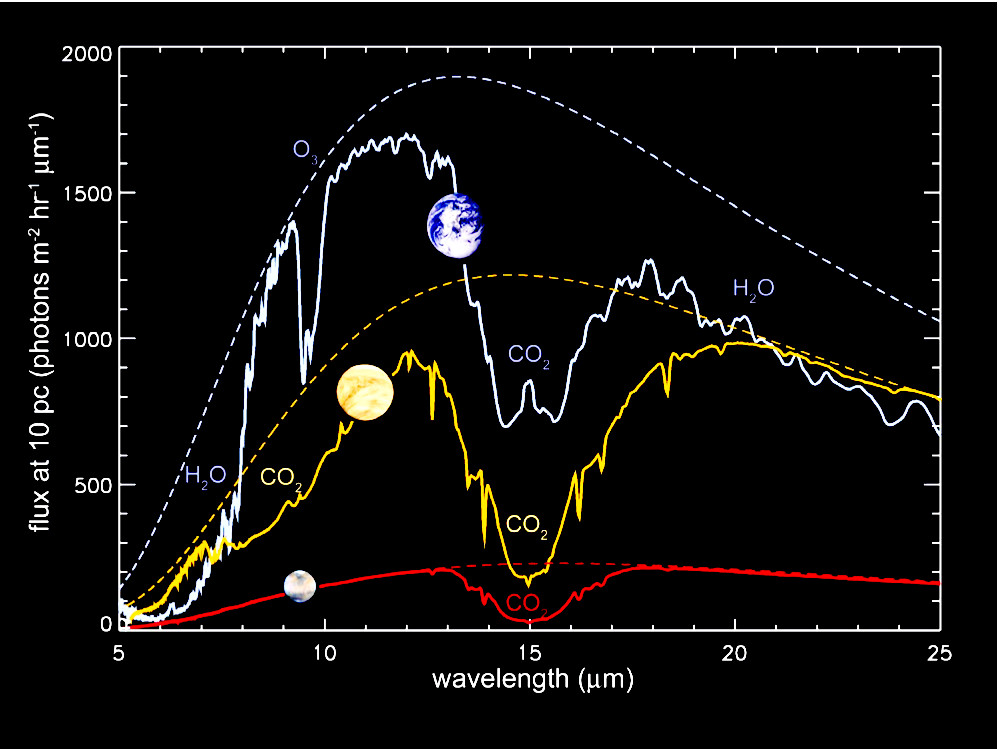
\includegraphics[width=.6\textwidth]{Astrofysik/billeder/venus-earth-mars_ir.jpg}
    \caption{Her ses spektre fra Jorden, Mars og Venus. De stiplede linjer angiver hvordan lyset ville være fordelt hvis ikke der skete absorption i atmosfæren.  \textit{Kilde: Franck Selsis and Giovanna Tinetti, Darwin proposal, 2007}} %https://light2015blogdotorg.wordpress.com/2015/03/02/searching-for-that-light-of-life/#more-756
    \label{fig:Biospektrer}
\end{figure}

\subsection*{Den Beboelige Zone}
For at finde genkendeligt liv, leder vi som sagt efter jordlignende planeter. Men hvilke krav skal vi stille til en planet, før den ligner os tilstrækkeligt?
Livet på Jorden er i høj grad baseret på kulstofforbindelser og vand. Man kunne muligvis også forestille sig liv baseret på kulstof og ammoniak eller silicium og ammoniak, men vi har aldrig fundet disse typer organismer. Livet på Jorden kan dog ikke klare sig med vand på hvilken som helst form - det kræver flydende vand. Så planeter der tillader flydende vand kan være særligt interessante.

Man har defineret et område omkring en stjerne kaldet "den beboelige zone", som ligger i den afstand fra stjernen, hvor en planet som Jorden kunne have flydende vand. Planetens atmosfære og masse har selvfølgelig betydning, men normalt vil man estimere zonen antaget en jordlignende planet. Er man for tæt på stjernen vil vandet fordampe, og er man for langt væk vil det fryse til is. Derfor er den beboelige zone tilpasset efter stjernens luminositet, så den er tæt på for små stjerner og langt væk for store stjerner. Et eksempel kan ses i figur \ref{fig:HZ}. At en planet er i den beboelige zone er dog bestemt ingen garanti for, at den er beboelig.

\begin{figure}[h!]
    \centering
    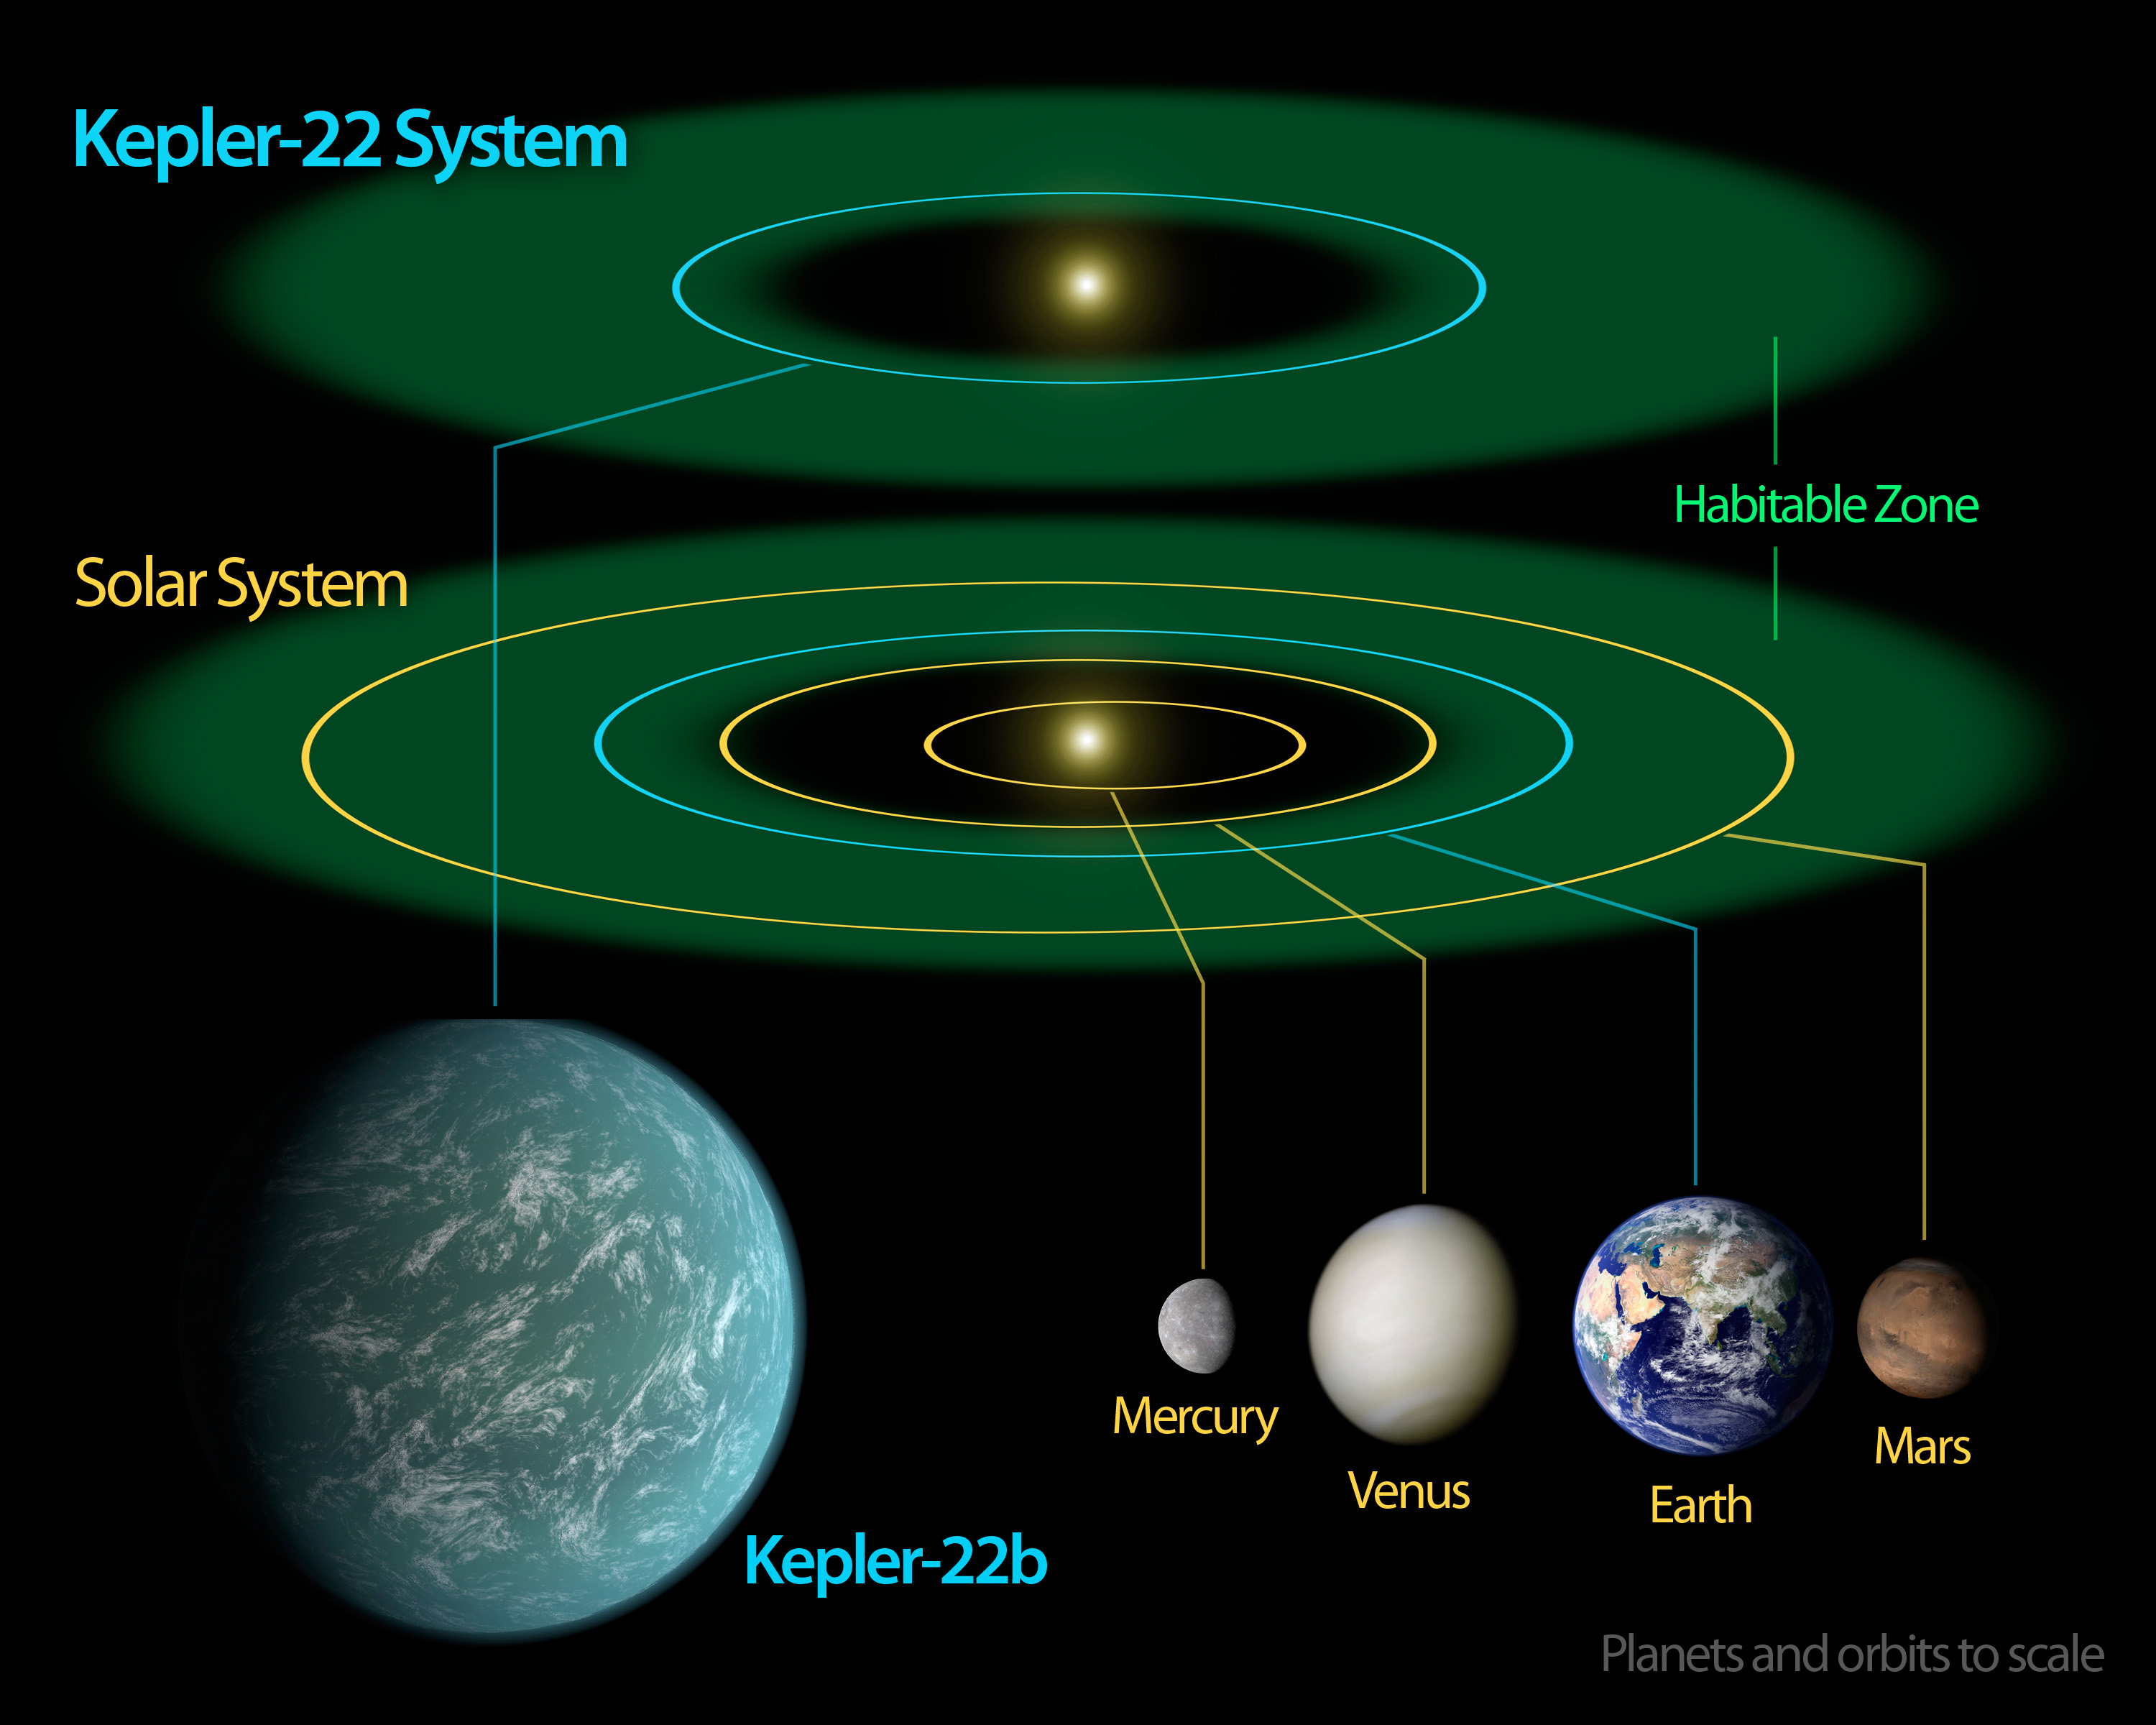
\includegraphics[width=.6\textwidth]{Astrofysik/billeder/Kepler-22_diagram.jpg}
    \caption{Illustration af et bud på den beboelige zone for Solsystemet og systemet om stjernen Kepler-22. 
    \textit{Kilde: https://commons.wikimedia.org/wiki/File:Kepler-22\_diagram.jpg}} %https://light2015blogdotorg.wordpress.com/2015/03/02/searching-for-that-light-of-life/#more-756
    \label{fig:HZ}
\end{figure}

%er den bedste taktik at lede efter en planet, der minder om Jorden, da der jo er liv her, men hvilke krav skal man stille til en såkaldt "jordlignende planet"? 
%Alt hvad vi kender til af liv på Jorden består hovedsageligt af organiske molekyler, og de interagerer på en eller anden led med molekyler som vand, ilt, kuldioxid og ammoniak. Vand er dog ikke bare vand, da liv ofte har det bedre i flyende vand, end is og vanddamp. 
Hvis man vil gå mere i dybden med om vand kan findes på den enkelte planet, kan man beregne dens overfladetemperatur, $T_p$, som
\begin{align} \label{eq:PlanetTemperatur}
    T_p = T_\star\left(\frac{1-A}{4}\right)^{1/4}\left(\frac{R_\star}{r}\right)^{1/2} \, ,
\end{align}
hvor $T_\star$ er stjernens overfladetemperatur, $R_\star$ er stjernens radius, $r$ er afstanden mellem stjernen og planeten og $A$ er planetens albedo. Albedoen er en enhedsløs konstant, der udtrykker hvor meget planeten reflekterer, da det jo kun er den energi planeten absorberer, der går til at varme den op. Denne formel bygger på en antagelse om, at der eksisterer en mekanisme, som fordeler energien på hele planetens overflade. Fx en hurtig rotationshastighed eller en atmosfære. Man kan også komme ud for at en planet er "låst" så den altid vender samme side mod Solen - i så fald vil den sandsynligvis være for varm på den ene side og for kold på den anden, men der kan være en stribe med lige den rette temperatur. Hvis der skal være flydende vand på planeten, så må $T_p$ være mellem $0$ og $\SI{100}{\degreeCelsius}$, under antagelse af nogenlunde atmosfærisk tryk. Dette illustrerer også hvor store dele af jagten på liv, der er præget af kvalificerede gæt og estimater. Hvis en planet har et tryk, der afviger meget fra \SI{1}{atm}, som vi har på Jorden, så vil temperaturintervallet, hvor vand kan eksistere i flydende form være helt anderledes eller måske ikke-eksisterende. Det er også en gråzone, hvis overfladetemperaturen jævnligt falder uden for intervallet. Det kunne fx ske hvis planetens bane er meget elliptisk, eller planeten blot er meget tæt på kanten af den beboelige zone. Det er derfor svært at sætte hårde krav til en planets afstand til sin stjerne. \\
Et andet problem med ligning \eqref{eq:PlanetTemperatur} er, at den bygger på, at planeten er i termodynamisk ligevægt, hvor den opvarmes af sin stjerne og nedkøles ved varmestråling. I Solsystemet findes der flere eksempler på, at der også er andre mekanismer i spil - fx overskydende varme i planetens indre og atmosfærer der holder på varmen. %Hvis en jordlignende planet befinder sig sådan ift. dens stjerne, at der kan eksistere flydende vand på overfladen af den, så siges planten at befinde sig i \emph{den beboelige zone}. 
\\

%Langt hen ad vejen er rummet et fantastisk vakuum, som man ikke umiddelbart skulle tænke som værende "farligt". Det er dog sådan at stjerner udsender en helt masse stråling, som er nødvendigt for eksempelvis at varme planeterne op til den nødvendige temperatur.
Selv hvis en stjernes lys er passende for flydende vand, er der andre krav for om liv også kan eksistere ved stjernen. Store stjerner lever kortere, og derved har livet formentlig ikke tid nok til at udvikles til avancerede former. Små stjerner er til gengæld meget aktive og har kraftige solvinde af partikler, der slynges ud mod planeterne. Disse består af ladede partikler med høj energi, der i værste fald kan blæse atmosfæren af en planet, hvis den ikke har et magnetfelt til at beskytte sig (og strålingen kan i sig selv være skadelig for liv at blive udsat for). Samtidig er den beboelige zone tæt på stjernen, hvis den er lille, så planeten ville blive påvirket endnu mere af solvindene. \\
%Jo højere energi strålingen har, desto mere destruktivt er det. Det kan ionisere og endda spalte ellers stabile molekyler. 
%Derudover er der også solvinde, som er en strøm af ladede partikler med ekstremt høj energi. Disse ladede partikler kan være elektroner, protoner eller heliumkerner og minder derfor om radioaktiv stråling. Forskellen er her at der er mange flere af dem og at de har ekstremt meget energi. Det der redder os på Jorden fra disse fænomener er Jordens magnetfelt og atmosfære. Uden disse ville vi ikke kunne overleve, da cellerne i kroppen ikke ville kunne klare det konstante strålingsbombardement - i stedet nøjes vi med at blive solbrændte. Derfor må det også kræves at en exoplanet kan opretholde en stabil atmosfære og gerne have et beskyttende magnetfelt. For at dette magnetfelt kan eksisterer må planeten på en eller anden led være opbygget af noget materiale, der er magnetisk i den tilstand det befinder sig i. \\

Planetens masse er også afgørende for om der kan eksistere liv, da tyngdekraften på overfladen af planeten hænger direkte sammen med massen. Hvis tyngdekraften er lidt svagere end på Jorden, kan man forvente højere organismer end her, og hvis tyngdekraften er stærkere vil det betale sig at være mere kompakt. Dette skyldes at en levende organisme skal være stabil, og jo stærkere tyngdekraften er, desto stærkere skal organismen også være, for at opretholde samme højde. Dette kan man forestille sig ved at tænke på, hvordan det føles at benytte en elevator. Når elevatoren accelereres opad presses man ned i gulvet, og når den så bremser ned igen, opnår man i kort tid en følelse af at være "lettere", hvilket blev vist teoretisk for et pendul i afsnit \ref{sec:elevator}. Denne analogi er helt valid, da en af byggestenene for den generelle relativitetsteori er Einsteins ækvivalensprincip, der kan formuleres som følgende:
\begin{center}
    \textit{Intet lokalt eksperiment kan skelne konstant acceleration og gravitation fra hinanden.}
\end{center}
Dette betyder, at i eksemplet med elevatoren er det umuligt at finde ud af om elevatoren står stille i et stærkere tyngdefelt, eller om den accelereres måske endda uden påvirkning af et tyngdefelt. \\
Der er en nedre grænse for, hvor lav planetens masse kan være, da den skal være stor nok til at kunne holde på en atmosfære - ellers vil den langsomt kunne fordampe væk. Mars lille størrelse er en af faktorerne, der har gjort, at den mistede sin. %Jordens atmosfære består af relativt små molekyler på gasform, hvorfor tyngdekraften skal have en vis styrke for at holde fast i disse. 
Er planeten for lille til at opretholde en atmosfære, vil der ikke være noget til at beskytte levende organismer og holde trykket for det flydende vand, hvilket vil gøre det umuligt, for det meste liv vi kender på Jorden at overleve. \\

Kobles massen sammen med radius til en densitet, kan vi også sætte begrænsninger på, hvad planeten kan bestå af, og det har betydning for hvilket liv der kan være. Jordens liv vil fx ikke have det særlig godt på en gasplanet. Hvis en planet er meget let, kan man godt konkludere at den må indeholde hydrogen, da intet andet ville kunne give så lav densitet. Der er også densiteter man vil forbinde med planeter af vand eller klippe. Hvis densiteten er meget høj må planeten også indeholde en vis mængde jern. \\
En anden metode til at undersøge en planets materiale er spektroskopi, som beskrevet i afsnit \ref{sec:spektrer} under spektrer. Ved at analysere spektret af en planet, kan man afgøre hvad den må bestå af.\\

%blev det beskrevet, hvordan stjerners sammensætning kan identificeres ud fra hvilke absorbtionslinjer, der observeres. Passerer lys igennem planetens atmosfære, vil der ske præcis det samme, som når lyset rejser igennem stjernen - atomerne og molekylerne interagerer med lyset. Molekyler interaktion med lys er en smule mere kompliceret end atomers interaktion, men det vigtige er at det er muligt at identificere molekyler ud fra deres spektre.\footnote{Forskellige typer spektre er essentielt i specielt mange dele af kemien, da forskellige præparater kan undersøges meget præcist. Det bruges eksempelvis i forbindelse kemisk syntese til at undersøge hvorvidt man faktisk har fremstillet det molekyle, man var interesseret i.} Hvis det er muligt at finde ud af hvordan spektret ville have set ud, hvis planeten ikke havde været der, så kan man identificere de absorbtionslinjer, der skyldes planetens atmosfære. Har man absorbtionslinjerne, kan man så identificere hvilke atomer og molekyler, disse stammer fra, selvom det nu er en del lettere sagt end gjort. Det bemærkes dog at denne metode til at bestemme atmosfæresammensætning, er afhængig af lys fra en kendt lyskilde passerer igennem planetens atmosfære. Derfor er det ikke muligt, hvis planeten kun kan "ses" med eksempelvis radialhastighedsmetoden, da det nødvendige lys ikke er tilgængeligt. \\

Er det så muligt at finde liv andre steder end på Jorden, eller er det hele blot en jagt på en ikkeeksisterende nål i en høstak af astronomisk størrelse? Det korte svar er, at det ikke er til at vide. Det kan være, at det venter lige om hjørnet, og at en af de kommende missioner til Mars finder rester af liv der. Det kan også være, at man kan lede til tid og evighed uden nogensinde at finde noget. Men ved at lede, kan vi i hvert fald sætte grænser for hvor almindeligt liv er, og hvor specielle forhold vi har. Mange forskere mener, at vi sandsynligvis vil finde liv inden for 10 år, hvis det eksisterer, i forbindelse med projekter der leder endnu grundigere end nu.
%Det er dog usandsynligt at svaret ligger gemt i en ligning, som i filmen \textit{Interstellar}. 
Jagten på liv er utroligt kompleks og fascinerende, hvilket forhåbentlig er illustreret i dette kapitel, men én ting er sikkert: Hvis man ikke leder efter nålen, så finder man den i hvert fald ikke.
%\section{Opgaver}
\begin{opgave}{God opgave}{1}

Find noget
\opg Udled ligning \ref{Pstar}.
\opg Og nu denne ting. Wow.
\end{opgave}


\begin{opgave}{Gravitationelle linser}{1}
Ligning, hvor man beregner hvornår der fokuseres mest
\opg Denne ting
\opg Og nu denne ting. Wow.

(Hint: Udnyt at noget andet gælder)
\end{opgave}

\begin{opgave}{Atmosfærekrav}{3}
For at en planet kan have en stabil atmosfære er den nød til at kunne holde simple molekyler fanget i dens tyngdefelt. Massen af $O_2$ er $m_{O_2} = \SI{5,31e-26}{\kilo\gram}$.
\opg Benyt Newtons gravitationslov og Newtons 2. lov til at bestemme tyngdeaccelerationen på en planets overflade.
\opg Er det legemes kinetiske energi præcis ligeså stor som dens gravitationelle potentielle energi, vil den kunne undslippe det tyngdefelt det befinder sig i. Vis at denne hastighed, kaldet undvigelseshastigheden fra en planet, er givet som
\begin{align*}
	v_\mathrm{ecs}^2 = \frac{2M_pG}{R_p}
\end{align*}
\opg Det oplyses nu fra kinetisk gasteori at
\begin{align*}
	\frac{1}{2}m\bar{v}^2 = \frac{3}{2}k_BT
\end{align*}
hvor $\bar{v}$ er partiklerne i gassens gennemsnitlige fart, $m$ er partiklernes masse, $k_B$ er Boltzmanns konstant og $T$ er temperaturen i Kelvin. \\
Vis at
\begin{align*}
	\frac{M_p}{R_p} = \frac{3}{2}\frac{k_BT}{mG}
\end{align*}
hvis $v_\mathrm{ecs} = \bar{v}$.
\opg Er $v_\mathrm{ecs} = \bar{v}$ vil op mod halvdelen af molekyler med massen $m$ forsvinde væk fra planeten. Konkluder at for at en exoplanet kan fastholde $O_2$ i sin atmosfære, skal der om planeten gælde at
\begin{align} \label{eq:atm}
	\frac{M_p}{R_p} > \frac{3}{2}\frac{k_BT}{m_{O_2}G}
\end{align}
\opg Den gennemsnitlige temperatur på Jorden antages at være \SI{16}{\degree}. Opfylder Jorden ligning \ref{eq:atm}?
\end{opgave}

\begin{opgave}{Gravitationslinser}{1}
I afsnit \ref{sec:GravLinse} om gravitationslinsemetode blev det nævnt at begivenheden skal observeres af flere forskellige målinger.
\opg Hvorfor er 1 måling ikke nok?
\opg Hvorfor er det usandsynligt at observere samme planet med gravitationslinsemetoden mere en én gang?
\opg Hvordan medfører ovenstående at planeten skal kunne ses i flere forskellige uafhængige målinger, for at kunne kaldes en planet?
\end{opgave}

\begin{opgave}{Bose-Einstein kondensat og laserkøling}{3}
For at lave Bose-Einstein kondensater i laboratoriet skal man have nogle lette partikler, der køles ekstremt meget ned.\footnote{For den interesserede læser er et Bose-Einstein kondensat at atomernes bølgefunktioner udvider sig, som temperaturen falder, indtil de sidst overlapper så meget at du får samme bølgefunktion. De kan derfor betragtes som én stor partikel.} Mere præcist køles atomer (ofte alkalimetaller) ned til ~\SI{.1}{\micro\kelvin}, hvilket gøres ved først laserkøling og senere fordampningskøling. Laserkøling fungerer ved at udnytte at fotoner har impuls. Rammes et atom af en foton, der bevæger sig i modsat retning af atomet, exciteres den til et højere energiniveau, men dens fart falder også en smule, for at bevare impulsen. Når atomet henfalder udsendes fotonen igen, og den accelereres en smule i en tilfældig retning. Sker dette mange gange går disse små accelerationer ud med hinanden over tid, hvorved atomet bremses og atomskyen køles. Det virker dog kun, hvis an kan sikre sig at atomer kun interagerer med fotoner, der bevæger sig i modsat retning af dem selv.
\opg Hvad er sammenhængen mellem en fotons energi og bølgelængde?
\opg Hvad sker der hvis et atom rammes af en foton med en energi, der ikke svarer til en (tilladt) atomar overgang? \textit{Hint: Tænk på atomet kvantemekanisk.} \\

Ved laserkølings sendes laserstråler ind fra seks retninger (positiv og negativ retning af hver af de kartesiske akser). Nu simplificeres systemet ved kun at kigge på systemet i én dimension. Betragt nu to ens atomer, der bevæger sig i hver sin retning. Fotonerne kommer fra en laser, der står stille i laboratoriet.
\opg Skiftes referencesystem til hvert atoms referenceramme, ser laseren ud til at bevæge sig. Hvorfor bevæger laseren sig ikke lige hurtigt i begge atomers referencesystem?
\opg Eftersom laseren bevæger sig Dopplerforskydes lyset. Hvad betyder forskellen i bevægelse for Doppllerforskydningen?
\opg Kan begge atomer exciteres af fotoner med samme bølgelængde?
\opg Hvordan kan dette bruges til at bremse atomerne selektiv?
\opg Er opgavetitlen clickbait?
\end{opgave}

\newpage\newpage
\setcounter{opgave}{0}

\section{Facit}
\begin{opgave}{Atmosfærekrav}{3}
For at en planet kan have en stabil atmosfære er den nød til at kunne holde simple molekyler fanget i dens tyngdefelt. Massen af $O_2$ er $m_{O_2} = \SI{5,31e-26}{\kilo\gram}$.
\opg Newtons gravitationslov siger at tyngdekraften mellem legemer i afstand $r$ er
\begin{align*}
	F_G = G\frac{mM}{r^2}
\end{align*}
Bruges Newtons anden lov er
\begin{align*}
	mg &= G\frac{mM}{r^2} \\
	g &= G\frac{mM}{r^2}
\end{align*}
hvor $g$ er tyngdeaccelerationen.
\opg Fra mekanik er de omtalte energier
\begin{align*}
	K &= \frac{1}{2}mv^2 \\
	V &= mgh
\end{align*}
hvor $h$ er afstanden fra nulpunktet. Defineres planetens centrum som nulpunktet er $h = R_p$, og sættes de to energi lig hinanden fås
\begin{align*}
	\frac{1}{2}mv^2 = mgR_p
\end{align*}
Isoleres $v^2$ før tyngdeaccelerationen fra før indsættes, fås
\begin{align*}
	v_\mathrm{ecs}^2 = \frac{2M_pG}{R_p}
\end{align*}
\opg I ligningen fra kinetisk gasteori isoleres $\bar{v}^2/2$
\begin{align*}
	\frac{1}{2}\bar{v}^2 = \frac{3}{2}\frac{k_BT}{m}
\end{align*}
Kombineres dette med undvigelseshastigheden fås
\begin{align*}
	\frac{3}{2}\frac{k_BT}{m} &= \frac{M_pG}{R_p} \\
	\implies \frac{M_p}{R_p} &= \frac{3}{2}\frac{k_BT}{mG}
\end{align*}
\opg Udtrykket på venstre side af lighedstegnet er egenskaber ved selve planten, mens udtrykket på højre side er egenskaber ved plantens atmosfære, der udtrykker partiklerne i atmosfærens hastighed. Hvis planeten skal kunne fastholde atmosfæren må den hastighed ikke overskride undvigelseshastigheden, hvorfor uligheden må være
\begin{align}
	\frac{M_p}{R_p} > \frac{3}{2}\frac{k_BT}{m_{O_2}G}
\end{align}
\opg For Jorden er forholdet mellem masse og radius
\begin{align*}
	\frac{M_\oplus}{R_\oplus} &= \frac{\SI{5,972e24}{\kilo\gram}}{\SI{6371}{\metre}} \\
	&= \SI{9.3737e+17}{\kilo\gram\per\metre}
\end{align*}
Sættes tallene ind i højresiden fås
\begin{align*}
	\frac{3}{2}\frac{k_BT}{m_{O_2}G} &= \frac{3\cdot\SI{1.38065e-23}{\joule\per\kelvin}\cdot(273,15 + 16)\SI{}{\kelvin}}{2\cdot\SI{5,31e-26}{\kilo\gram}\cdot\SI{6.67408e-11}{\metre\cubed\per\kilo\gram\per\second\squared}} \\
	&= \SI{1.6886e+15}{\kilo\gram\per\metre}
\end{align*}
Ergo er ligningen opfyldt for Jorden.
\end{opgave}

\begin{opgave}{Gravitationslinser}{1}
I afsnit \ref{sec:GravLinse} om gravitationslinsemetode blev det nævnt at begivenheden skal observeres af flere forskellige målinger.
\opg Kigges der ud i verdensrummet er der mange ting der kan ses. En lyskurve, som beskrevet i afsnittet, kan også skyldes andre fænomener, skyldes en fejl i målingerne, eller bare et statistisk udsving. For at man kan konkludere noget naturvidenskabeligt, så er man derfor nød til at observere det samme fænomen på en sådan måde, sådan så der kun er en realistisk konklusion.
\opg Gravitationslinsemetoden kræver en meget specifik situation, netop at en stjerne med tilhørende planten bevæger sig ind foran en anden stjerne alt samme i et plan, hvori Jorden også er. For at "lensingen" kan ske er de to stjerne separeret af en anseelig afstand, hvorfor de ikke nødvendigvis påvirker hinanden gravitationelt signifikant. Det er derfor meget muligt at begivenheden kun forekommer én gang, og hvis den ene stjerne er i bane om den anden, så er perioden så kæmpe stor at det er urealistisk at vente lang nok tid til at se det igen.
\opg Hvis man kun har én mulighed for at observere begivenheden, men stadig vil kunne afvise at det er er andet end en planet, så er man for det første nød til at have så mange målinger med forskelligt udstyr, at man kan afvise at der er tale om en fejl i målingerne eller en statistisk afvigelse fra normen. Derudover er man også nød til på en eller anden måde at kunne verificere at det ikke kan skyldes andre fænomener. Den bedste måde at gøre dette på er at observere systemet i lang tid før og efter, med flere forskellige instrumenter, så man ved hvordan området på stjernehimlen normalt ser ud.
\end{opgave}

\begin{opgave}{Bose-Einstein kondensat og laserkøling}{2}
\opg $E = \frac{hc}{\lambda}$ hvor $h$ og $c$ er konstanter, hvorfor energien bliver større, hvis bølgelængden bliver kortere
\opg Ingenting (ideelt set), da atomets energiniveauer er kvantiseret, hvorfor der ikke kan ske noget, hvis ikke fotonens energi er lige præcis nok til at to at flytte elektronen fra ét energiniveau til et andet.
\opg For at holde styr på atomerne kaldes den der bevæger sig mod laseren (1), og den der bevæger sig væk fra (2). Kaldes retningen af atom (1) for den positive retning, gælder følgende: \\
(1) Laseren bevæger sig mod atomet, og altså i negativ  retning. \\
(2) Laseren bevæger sig væk fra atomet, og altså i positiv retning.
\opg Der kigges nu på samme foton fra de to referencesystemer. \\
(1) Fotonen er udsendt fra en kilde, der bevæger sig mod atomet, hvorfor fotonen er blåforskydt. \\
(2) Fotonen er udsendt fra en kilde, der bevæger sig væk fra atomet, hvorfor fotonen er rødforskydt.
\opg De to atomer ser ikke fotonen, som havende samme bølgelængde, og dermed ikke samme energi. Da atomerne er ens, har de samme energiniveauer, men da atomerne oplever fotonen forskelligt, så passer fotonen ikke med en overgang i begge atomer.
\opg Atomet skal gerne holdes samlet i midten af den fælde, hvori de holdes. De atomer, der bevæger sig væk fra fælden mod laseren ser laseren som blåforskudt. Vælges laserens til at have en bølgelængde, der er lidt længere end den, der svarer til overgangen hvis atomet står stille. Det betyder at kun atomer på vej ud af fælden oplever lyset, som værende Dopplerforskudt på den måde, der gør det muligt for atomet at interagere med lyset. Derved kan man sikre sig at man kun påvirker de rigtige atomer, og derved køler gassen.
\opg Dette kan opgavens forfatter ikke besvare. Ifølge JR er svaret entydigt "ja"!
\end{opgave}

\chapter{Atom- og Molekylefysik}\label{cha:AMO}
%\subfile{Atom-ogMolekylefysik/Sections/A.Intro.tex}
%\subfile{Atom-ogMolekylefysik/Sections/B.3D.tex}
\subfile{Atom-ogMolekylefysik/Sections/C.Atomstruktur.tex}
\subfile{Atom-ogMolekylefysik/Sections/D.L-S.tex}
\subfile{Atom-ogMolekylefysik/Sections/E.Hyperfin.tex}
%\subfile{Atom-ogMolekylefysik/Sections/F.Zeeman.tex}
\subfile{Atom-ogMolekylefysik/Sections/G.DIC.tex}
%\newpage
%\twocolumn
%\section{Opgaver}
%\subfile{Atom-ogMolekylefysik/opgaver/1.ombytning.tex}
%\subfile{Atom-ogMolekylefysik/opgaver/2.Finstruktur.tex}
%\subfile{Atom-ogMolekylefysik/opgaver/3.Hyperfinstruktur.tex}

%\onecolumn
%\newpage
%\twocolumn
%\section{Facit}
%\setcounter{opgave}{0}
%\subfile{Atom-ogMolekylefysik/opgaver/facit/finstruktur.tex}

%\onecolumn
%\chapter{Appendix}
%\subfile{Atom-ogMolekylefysik/Sections/Z-appendix.Hydrogen.tex}
%\subfile{Atom-ogMolekylefysik/Sections/Y-appendix.punktgrupper.tex}

\chapter{Planetbevægelse}\label{cha:Planet}
I dette kapitel skal vi undersøge klassisk bevægelse i stjernesystemer. Specifikt skal vi kigge på Keplers love og ud fra Lagrangemekanik undersøge, hvordan planeter, kometer og lignende bevæger sig omkring tungere objekter såsom stjerner. Vi vil tage udgangspunkt i det generelle tolegemeproblem, hvor to legemer påvirker hinanden med en indbyrdes centralkraft. Herefter vil vi kigge på det særlige tilfælde, hvor denne kraft er omvendt proportional med afstanden imellem de to legemer kvadreret, og til sidst sætter vi denne kraft til at være tyngdekraften. Til dette vil vi introducere keglesnit og vise, at bevægelserne der fremkommer kan beskrives ud fra de geometriske former, der fås ved at snitte en kegle på forskellige måder.


\section{Planetbaner og excentricitet}
Når objekter er i bevægelse om et centralt legeme, for eksempel en planet omkring en stjerne, kan deres baner generelt have tre forskellige former: Elliptiske, parabolske og hyperbolske. Formen af disse afhænger af banernes excentricitet $\epsilon$, som beskriver, hvor tæt banerne er på at være perfekt cirkelformede.

\subsection{Excentricitet fra keglesnit}
\begin{figure}[h!]
	\centering
	\begin{subfigure}{0.45\textwidth}
		\centering
		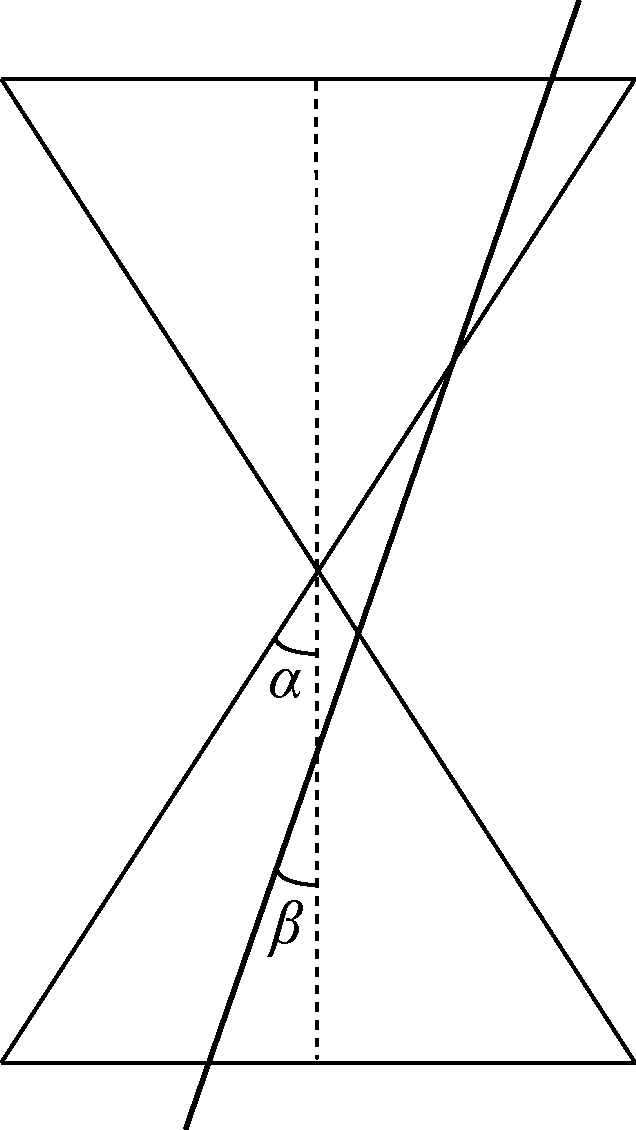
\includegraphics[width=0.55\textwidth]{Planetbevaegelse/KeglePlan.pdf}
		\caption{En dobbeltkegle med vinkel $\alpha$ til den horisontale akse (stiplet linje) skæres af et plan (breddere linje) med en vinkel $\beta$ til den vertikale akse.}
		\label{fig:KeglePlan}
	\end{subfigure}
	\hspace{5mm}
	\begin{subfigure}{0.45\textwidth}
		\centering
		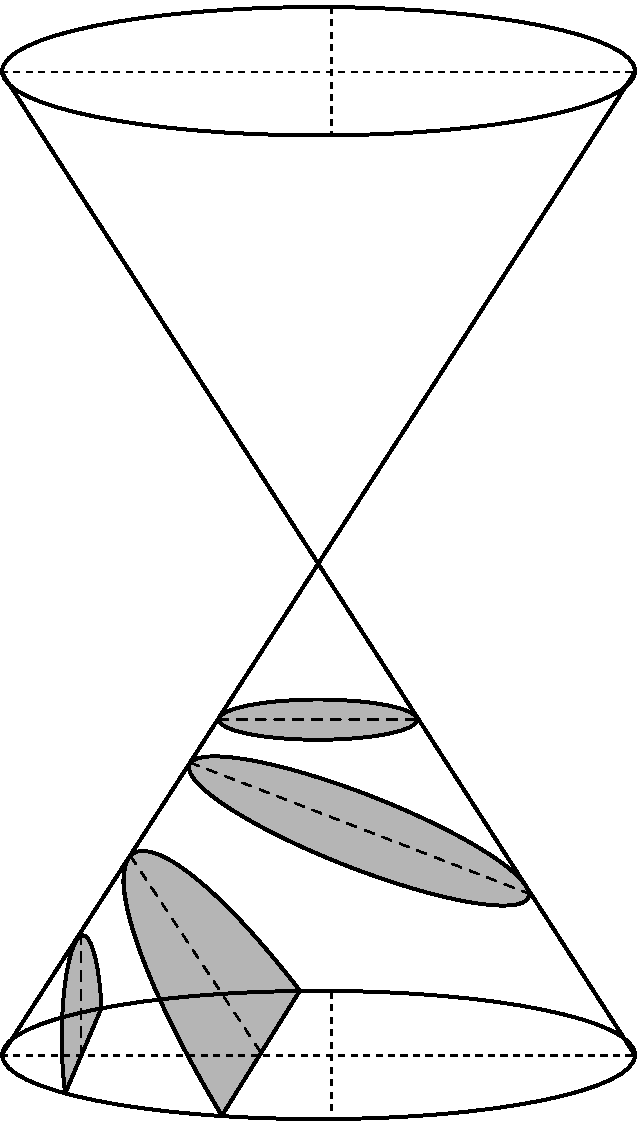
\includegraphics[width=0.55\textwidth]{Planetbevaegelse/KegleOrbit.pdf}
		\caption{Banerne fremkommer ved keglesnit med forskellige vinkler (fra øverst): Cirkel ($\epsilon = 0$), ellipse ($0 < \epsilon < 1$), parabel ($\epsilon = 1$) og hyperbel ($\epsilon > 1$).}
		\label{fig:KegleOrbit}
	\end{subfigure}
	\caption{En dobbeltkegle og dens keglesnit, som resulterer i forskellige planetbaner.}
\end{figure}

Ses på en dobbeltkegle dannet af en ret linje, der roterer omkring en fastlåst akse, og et plan der skærer denne kegle, figur \ref{fig:KeglePlan}, da kan excentriciteten af det keglesnit, der opstår, beskrives ved
\begin{align}
	\epsilon &\equiv \frac{\cos(\beta)}{\cos(\alpha)} \: .
\end{align}
Her betegner $\alpha$ og $\beta$ vinklen mellem den horisontale akse i keglen og henholdsvis keglesiden og planet. For $\alpha$ og $\beta$ skal det gælde, at $0<\alpha<\pi/2$, da keglen skal være en kegle og ikke blot en vertikal eller horisontal linje, og $0 \le \beta \le \pi/2$, da planet må være alt fra og med vertikalt til og med horisontalt.
Nogle af de keglesnit der fremkommer ved dette, kan ses på figur \ref{fig:KegleOrbit}, og de fremkommer på følgende måder:
\begin{itemize}
	\item \textbf{Elliptiske baner:} Idet planet skærer keglen i en vinkel større end keglens vinkel\footnote{Dette afsnit gør sig gældende så længe, at planet ikke skærer dobbeltkeglen i samlingspunktet mellem de to kegler, altså hvor de to kegles spidser mødes, da der så ville være tale om degenererede keglesnit.}, således at $\beta > \alpha$, vil elliptiske baner forekomme, da planet skærer begge sider af keglen, hvorfor banen er lukket. Excentriciteten af disse baner bliver derved $\epsilon < 1$. Cirkelbaner er et specialtilfælde af de elliptiske baner, hvor excentriciteten er $\epsilon = 0$.
	\item \textbf{Parabolske baner:} Når planet skærer keglen i en vinkel lig keglens vinkel, $\alpha = \beta$, opstår en parabolsk bane. Siden denne bane er parallel med keglesiden, vil denne være grænsen mellem lukkede og åbne baner. Excentriciteten af sådanne baner er $\epsilon = 1$.
	\item \textbf{Hyperbolske baner:} Tilbage er når planet skærer dobbeltkeglen i en vinkel mindre end keglens vinkel, så $\beta < \alpha$, hvorved der dannes en hyperbolsk bane, da planet kun skærer hver af keglerne i dobbeltkeglen ét sted, hvorfor der dannes en åben bane. Ud fra de givne vinkler er excentriciteten af en hyperbolsk bane givet ved $\epsilon > 1$.
\end{itemize}

\subsection{Fysisk definition af excentricitet}
\begin{figure}[h!]
	\centering
	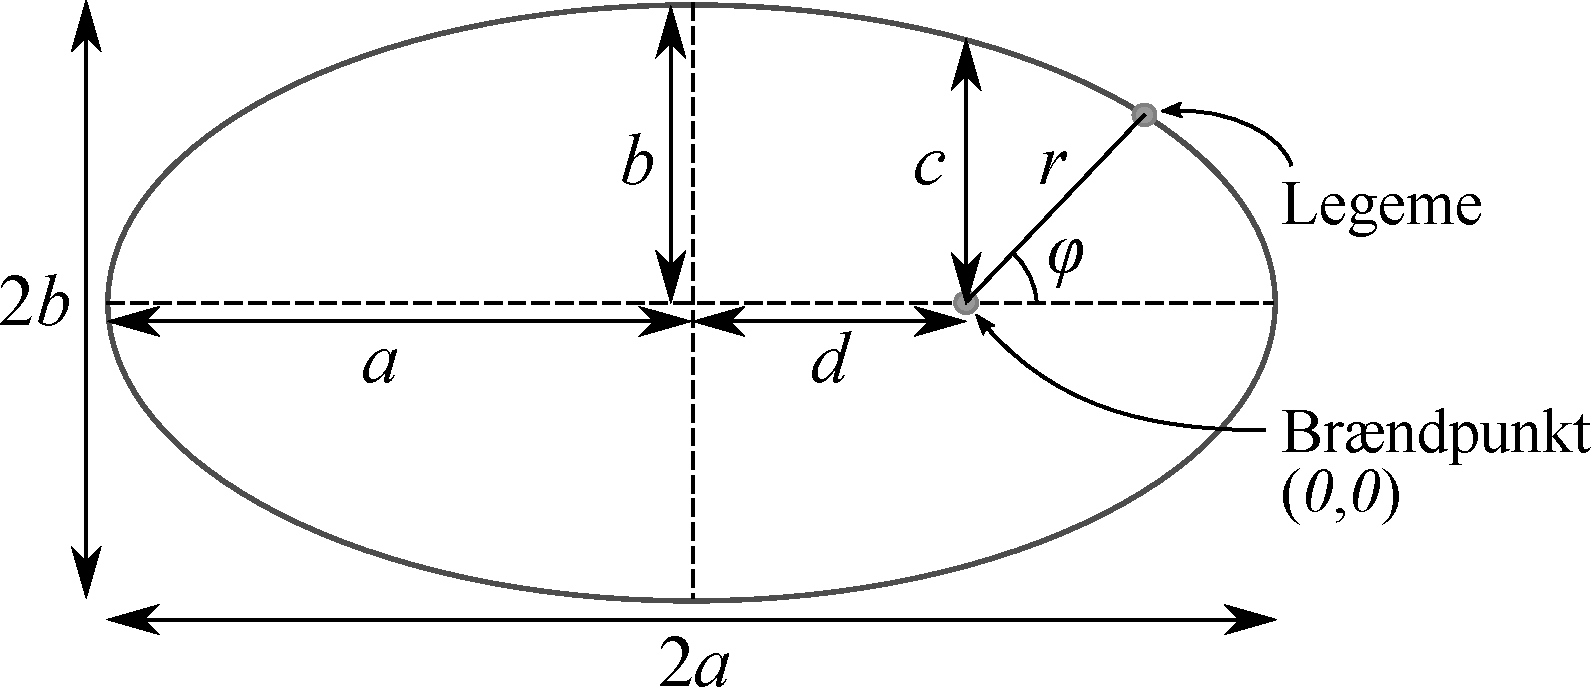
\includegraphics[scale=0.45]{Planetbevaegelse/Ellipse.pdf}
	\caption{Elliptisk bane hvor $a$ og $b$ betegner henholdsvis den halve storakse og den halve lilleakse, $d$ er forskydningen af brændpunktet fra ellipsens centrum, $c$ er afstanden af et linjestykke fra brændpunktet til punktet på ellipsen, hvor dette linjestykke er vinkelret på storaksen, og $r$ er afstanden fra brændpunktet til et virkårligt sted på ellipsen i en vinkel $\phi$. Ved udregninger antages brændpunktet at ligge i $(0,0)$.}
	\label{fig:Ellipse}
\end{figure}

Mens denne beskrivelse af excentricitet virker fint til matematisk at beskrive ellipser, parabler og hyperbler, da er den ikke specielt brugbar til beregning af excentriciteten af planetbaner, da man ikke har en kegle i rummet at gå ud fra. Af denne grund findes en anden og ækvivalent definition af excentricitet, som tager udgangspunkt i de parametre, som kan måles for en planetbane:
\begin{align}
	\epsilon &\equiv \frac{d}{a} \: .
\end{align}
Her er $a$ den halve storakse, og $d$ er afstanden fra et brændpunkt til centrum af banen, se figur \ref{fig:Ellipse}. \\
\noindent
Excentriciteten af en planetbane bruges til at beregne afstanden mellem to objekter, hvor det ene objekt befinder sig i bane om det andet i vilkårlig vinkel $\phi$, som angivet på figur \ref{fig:Ellipse}. Ligningen for banens radius, som funktion af vinklen af et objekt, ligning \eqref{eq:Ellipse_i_polaere_koordinater}, kan findes ved at konvertere formlerne for en elliptisk bane med nulpunkt i et brændpunkt, ligning \eqref{eq:Ellipse_i_kartesiske_koordinater}, en parabolsk bane, ligning \eqref{eq:Parabel_i_kartesiske_koordinater}, og en hyperbolsk bane, ligning \eqref{eq:Hyperbel_i_kartesiske_koordinater}, fra kartesiske koordinater:
\begin{align}
	1 &= \frac{(x+d)^2}{a^2} + \frac{y^2}{b^2} \label{eq:Ellipse_i_kartesiske_koordinater} \\
	y^2 &= c^2 - 2cx \label{eq:Parabel_i_kartesiske_koordinater} \\
	1 &= \frac{(x-\delta)^2}{\Gamma^2}-\frac{y^2}{\eta^2} \: , \label{eq:Hyperbel_i_kartesiske_koordinater}
\end{align}
hvor $a$, $b$ og $d$ er givet ved følgende formler:
\begin{equation} \label{eq:Planetbevaegelse_a_b_og_d}
	\begin{aligned}
		a &= \frac{c}{1-\epsilon^2} \\
		b &= \frac{c}{\sqrt{1-\epsilon^2}} \\
		d &= a\epsilon \: ,
	\end{aligned}
\end{equation}
og $\Gamma$, $\delta$, $\eta$ og $c$ er konstanter, til polære koordinater. Dette viser sig at give én og samme ligning
\begin{align} \label{eq:Ellipse_i_polaere_koordinater}
	r(\phi) &= \frac{c}{1+\epsilon\cos(\phi)} \: ,
\end{align}
hvilken vi senere viser at planetbaner opfylder.

\section{Tolegemeproblemet}
Til at udlede Keplers love, er det relevant at kende lidt mere til det problem vi arbejder med. Vi starter med et mere generelt tilfælde, end det vi vil undersøge, nemlig det generelle tolegemeproblem. Det er et system hvor følgende er opfyldt: Systemet skal indeholde præcis to legemer, der påvirker hinanden med en indbyrdes central, konservativ kraft. At kraften er central betyder, at den udelukkende afhænger af afstanden mellem de to legemer. At den er konservativ betyder, at arbejdet den udfører på et af legemerne, ikke afhænger af vejen taget, men kun af start- og slutpunkt for vejen.\\
Vi kigger på to legemer med massen $m_1$ og $m_2$, der betragtes som punktpartikler, se figur \ref{fig:planet_relativ}. Vi opskriver først systemet, som et inertialsystem, det vil sige et system, der bevæger sig med konstant hastighed i forhold til alle andre inertialsystemer. Dette system kan betragtes som værende i hvile, og det må ikke være roterende. I et inertialsystem har hvert legeme en vektor, der går fra origo og ud til legemet, henholdsvis $\subv{r}{1}$ og $\subv{r}{2}$. Legemerne påvirkes af en fælles tiltrækningskraft, henholdsvis $\subv{F}{21}$ og $\subv{F}{12}$, som antages at være konservativ og central. Da kræfterne er konservative, kan de udledes fra en potentiel energi $V(\subv{r}{1},\subv{r}{2})$. Vi vil senere sætte denne kraft til at være en gravitations kraft af størrelsen, $Gm_1m_2/|\subv{r}{1}-\subv{r}{2}|^2$, med tilhørende potentiel energi
\begin{align}
	V(\subv{r}{1},\subv{r}{2}) = -\frac{Gm_1m_2}{|\subv{r}{1}-\subv{r}{2}|}.
\end{align}
Bemærk her, at den potentielle energi kun afhænger af afstanden mellem legemerne, og ikke de individuelle vektorer. Dette er hvad det vil sige, at kraften er central, og det betyder også, at den potentielle energi ikke afhænger af hvilket inertialsystem, vi vælger. Potentielle energier, med denne egenskab, kaldes translationelt invariante. Det er altså lige meget for kraften og den potentielle energi, hvor origo ligger. \\
%
Der gælder derved nærmere, at $V(\subv{r}{1},\subv{r}{2}) = V(|\subv{r}{1}-\subv{r}{2}|)$, og det giver mening at introducere en ny vektor, $\v{r}$, som vi kalder den relative position:
\begin{align}
	\v{r} = \subv{r}{1}-\subv{r}{2}.
\end{align}
Afstanden imellem de to legemer, $r$, er således størrelsen af vektoren $\v{r}$, og $V=V(r)$. \\ \\
% Sæt figur op
%
\begin{figure}[h!]
\centering
	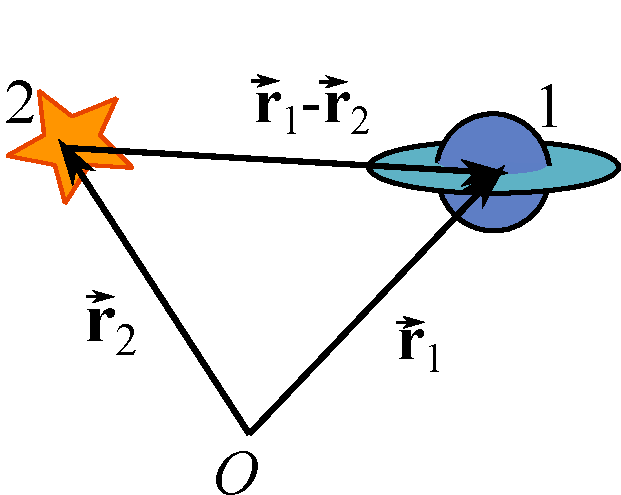
\includegraphics[width = 0.4\textwidth]{Planetbevaegelse/relativkoordinat_planet.pdf}
	\caption{Illustrerer vektorer $\v{r}_1$ og $\v{r}_2$ fra origo til hver af de to legemer, samt den relative positionsvektor $\v{r} = \v{r}_1 - \v{r}_2$ af legeme 1 i forhold til legeme 2.}
	\label{fig:planet_relativ}
\end{figure}
Nu kan problemets Lagrangefunktion opskrives:
\begin{equation}
\begin{aligned}
	L &= \frac{1}{2} m_1 \dt{\v r}_1^2 + \frac{1}{2} m_2 \dt{\v{r}}_2^2 - V(r) \\
	&= \frac{1}{2} m_1 \dt{\v{r}}_1^2 + \frac{1}{2} m_2 \dt{\v{r}}_2^2 + \frac{Gm_1m_2}{r}.
\end{aligned}
\end{equation}
Dette kunne også være opskrevet ud fra Newtons love, men i dette tilfælde holder vi os til vores nyligt lærte Lagrangemekanik.


\section{Massemidtpunkt, relative koordinater og reduceret masse}
Vi skal vælge hvilke generaliserede koordinater, vi vil opskrive og løse systemet i. Indtil videre har vi bare opskrevet problemet i et almindeligt inertialsystem med kartesiske koordinater og et vilkårligt nulpunkt. \\
%
Dog lægger systemet tydeligvis op til at man benytter et relativ koordinat, $\v{r}$, som en af vores generaliserede koordinater. Da systemet er centralt og kun involverer to legemer og kræfter, der følger en lige linje, behøver vi ikke mere end et 3-dimensionelt koordinat til hvert legeme\footnote{de oprindelige koordinater er $\subv{r}{1}$ og $\subv{r}{2}$}. Så indtil videre skal der bruges et koordinat mere, for at vi har lige så mange koordinater, som forventede frihedsgrader. Her vælges et koordinat, kaldet massemidtpunktet, eller "centre of mass coordinate"\;(med endepunkt CM), som betegnes $\v{R}$. Den er defineret som
\begin{align}\label{CM}
	\v{R} &= \frac{m_1 \subv{r}{1} + m_2 \subv{r}{2}}{m_1 + m_2} = \frac{m_1 \subv{r}{1} + m_2 \subv{r}{2}}{M} \, ,
\end{align}
hvor $M$ betegner den totale masse for systemet: $M = m_1 + m_2$. Da $\v{R}$ involverer en sum af de vægtede vektorer, viser det sig, at massemidtpunktet ligger på linjen mellem de to legemer, dannet af $\subv{r}{1} - \subv{r}{2}$. \\

%Figur 
%
\begin{figure}[h!]
\centering
	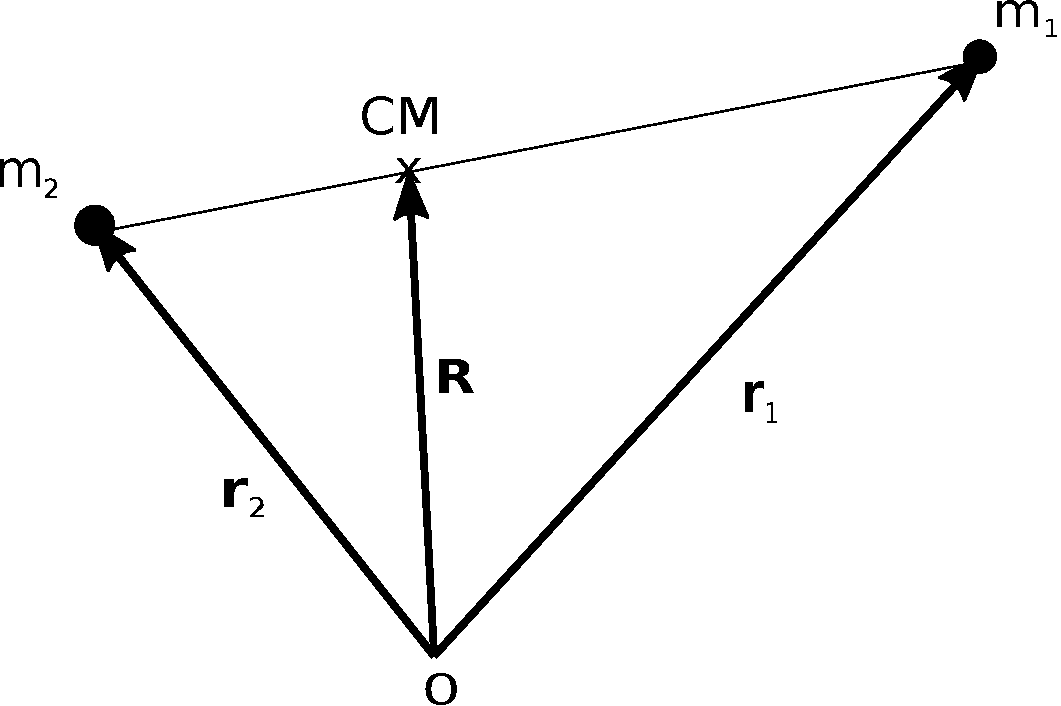
\includegraphics[width = 0.4\textwidth]{Planetbevaegelse/figur_CM.pdf}
	\caption{Massemidtpunktet for de to legemer ligger ved $\v{R} = (m_1 \v{r}_1 + m_2 \v{r}_2)/M$ på linjen mellem de to legemer.}
\end{figure}
Den totale impuls, $\v{P}$, for systemet er den samme, som den totale masse lagt til ændringsraten for $\v{R}$ i tiden:
\begin{align}
	\v{P} &= \dif{t}{} \left( m_1 \subv{r}{1} + m_2 \subv{r}{2} \right) = M \dt{\v{R}} .
\end{align}
Den totale impuls for systemet er konstant, da systemet ikke påvirkes af udefrakommende kræfter. Derfor må $\dt{\v{R}}$ være konstant, og der findes således et inertialsystem hvor $\dt{\v{R}}=\v{0}$ (inertialsystemer er systemer, der ikke accelererer). \\ \\
%
%
For at kunne introducere $\v{r}$ og $\v{R}$ som generaliserede koordinater i Lagrangefunktionen skal den kinetiske og potentielle energi omskrives til at være afhængig af dem, i stedet for de gamle koordinater. Vi ved allerede, at den potentielle energi let kan skrives, som afhængende kun af den relative afstand $r$. For den kinetiske energi skal vi først omskrive $\subv{r}{1}$ og $\subv{r}{2}$ til at afhænge af vores generaliserede koordinater. Fra definitionen af $\v{R}$ i ligning~\eqref{CM}, kan $\subv{r}{1}$ isoleres, og ved introduktion af definitionen af $\v{r}$ fås:
\begin{align}\label{Eq:r1}
	\subv{r}{1} = \v{R} + \frac{m_2}{M}\v{r}.
\end{align}
Det samme kan gøres med $\subv{r}{2}$, hvor der fås:
\begin{align}\label{Eq:r2}
	\subv{r}{2} = \v{R} - \frac{m_1}{M} \v{r}.
\end{align}
Den kinetiske energi bliver så:
\begin{equation}
\begin{aligned}
	K &= \frac{1}{2}(m_1 \dt{\v r}_1^2 + m_2 \dt{\v r}_2^2 ) \\
	  &=\frac{1}{2} \left(m_1 \left[\dt{\v{R}} + \frac{m_2}{M}\dt{\v{r}} \right]^2 + m_2 \left[\dt{\v{R}} - \frac{m_1}{M} \dt{\v{r}}\right] ^2 \right) \\
	  &= \frac{1}{2} \left( M \dt{\v{R}}^2 + \frac{m_1m_2}{M}\dt{\v{r}}^2\right),
\end{aligned}
\end{equation}
som reduceres yderligere til 
\begin{align}
	K = \frac{1}{2} M \dt{\v{R}}^2 + \frac{1}{2} \mu \dt{\v{r}}^2 \, ,
\end{align}
ved introduktion af en såkaldt "reduceret masse"\;$\mu$. Parameteren $\mu = \frac{m_1m_2}{M}$ har enheder af masse. \\
%
I de generaliserede koordinater er den kinetiske energi det samme, som en traditionel kinetisk energi for to "fiktive"\;partikler, en med massen $M$, der bevæger sig med samme hastighed som CM, og en med masse $\mu$, der bevæger sig med samme hastighed, som den relative position $\v{r}$. Derfor kan den samlede Lagrangefunktion splittes op i to dele, en for den relative bevægelse, og en for CM-bevægelsen:
\begin{equation}
\begin{aligned}
	L = K - V &= \frac{1}{2} M \dt{\v{R}}^2 + \left( \frac{1}{2}\mu \dt{\v{r}}^2 - V(\v r)\right) \\
	&= L_\text{CM} + L_\text{rel}.
\end{aligned}
\end{equation}
Derved kan de to koordinater løses som to separate problemer.
%
%
\section{Bevægelsesligningerne}
Ud fra den opskrevne Lagrangefunktion kan bevægelsesligningerne for systemet findes. Fra hovedemnet om Lagrangemekanik har vi Euler-Lagrange relationerne, ligning~\eqref{Euler-Lagrange}. Ved at benytte dem fås først bevægelsesligningerne for $\v{R}$ (bemærk her at $\v{R}$ teknisk set er en tre-dimensionel vektor, så der er tale om tre ligninger, for $X$, $Y$ og $Z$, som ellers er ens\footnote{Med ens menes der, at alle operationer vi benytter påvirker de tre koordinatligninger ens.}). Da Lagrangefunktionen ikke direkte afhænger af $\v{R}$ giver Euler-Lagrangeligningen i forhold til koordinatet $\v{R}$ at:
\begin{align}
	M\ddt{\v{R}} = \v{0},
\end{align}
som betyder, at $\dt{\v{R}}$ er konstant. Dette er allerede forklaret med, at den totale impuls for systemet er bevaret. Det kan også forklares ud fra, at Lagrangefunktionen er uafhængig af $\v{R}$, hvorfor der er tale om et negligibelt koordinat. Nærmere opfører $L_\text{CM}$ sig som en Lagrangefunktion for en fri partikel, med masse $M$ og position $\v{R}$. At det er et negligibelt koordinat betyder i sidste ende, at vores system nødvendigvis kun har en enkelt frihedsgrad, fremfor de to, som var forventet. \\ \\
%
%
Hvis Euler-Lagrangerelationen anvendes med hensyn til den 2. koordinat, $\v{r}$, fås:
\begin{align}
	\mu \ddt{\v{r}} &= - \grad{V(\v r)} = - \xyz{\partial V / \partial x}{\partial V / \partial y}{\partial V / \partial z} = \subv{F}{res}.
\end{align}
At gradienten af den samlede potentielle energi på et af legemerne, $\grad{V}$, er lig den resulterende kraft på legemet op til et fortegn, blev kort nævnt i mekanikkapitlet, men skyldes udelukkende, at vi kun arbejder med konservative kræfter. \\ \\
%
%
For at få bevægelsesen for det relative koordinat skal vi bare løse Newtons 2. lov for en enkelt partikel med reduceret masse $\mu$ og position $\v{r}$, i et potentiale $V(\v r)$.
%
%
\subsection*{Massemidtpunktsreferencesystemet}
Vi kan vælge et inertialsystem hvori $\dt{\v{R}} = \v{0}$, netop fordi $\dt{\v{R}}$ er konstant. Her vil den totale impuls for systemet være nul, og $L_\text{CM} = 0$. Derved bliver vores Lagrangefunktion
\begin{align}
	L = L_\text{rel} = \frac{1}{2} \mu \dt{\v{r}}^2 - V(\v r).
\end{align}
Problemet er reduceret til et etlegemeproblem, hvilket også var forventet, siden $\v{R}$ var et overflødig koordinat. \\ \\ % Lav en figur der viser bevægelsen i vores referencesystem

\subsection{Bevaring af impulsmoment}
Da der ikke er udefrakommende kræfter på systemet, må det, udover at betyde at totalimpulsen er bevaret, også betyde, at det totale impulsmoment (\textit{angular momentum}) også er bevaret. Det totale impulsmoment vil, ud fra de to oprindelige koordinater $\subv{r}{1}$ og $\subv{r}{2}$, være summen af de to legemers impulsmoment:
\begin{align}
	\v{L} &= \subv{r}{1} \times \subv{p}{1} + \subv{r}{2} \times \subv{p}{2} = \v r_1 \times m_1\dt{\v r}_1+\v r_2 \times m_2\dt{\v r}_2 \: .
\end{align}
Der benyttes her symbolet $\v{L} = \v{\ell}_1 + \v{\ell}_2$ for det totale impulsmoment, fordi man med ved brug af et stort bogstav indikerer, at der er tale om en sum af samme fysiske størrelse for flere legemer. I CM-referencesystemet, hvor origo er valgt til $\v{R} = \v 0$, fås specifikt fra ligningerne~\eqref{Eq:r1} og \eqref{Eq:r2} at:
\begin{align}
	\subv{r}{1} &= \frac{m_2}{M}\v{r} \\
	\subv{r}{2} &= -\frac{m_1}{M}\v{r}.
\end{align}
Derved fås, at det totale impulsmoment bliver:
\begin{equation}
\begin{aligned}
	\v{L} &= \frac{m_1 m_2}{M} \v{r} \times \frac{m_2}{M} \dt{\v{r}} - \frac{m_2 m_1}{M} \v{r} \times \left(-\frac{m_1}{M}\right) \dt{\v{r}} \\
	&= \frac{m_1m_2}{M^2}\left(m_2\v{r} \times \dt{\v{r}} + m_1 \v{r} \times \dt{\v{r}}\right) \\
	&= \v{r} \times \mu \dt{\v{r}}.
\end{aligned}
\end{equation}
hvor $m_1m_2/M$ er erstattet med den reducerede masse $\mu$. Herved ser vi også, at det totale impulsmoment for systemet i CM systemet svarer til det ækvivalente impulsmoment for en enkelt partikel med massen $\mu$ og positionen $\v{r}$. Da det totale impulsmoment er bevaret, må vektoren $\v{r} \times \dt{\v{r}}$ være konstant i både størrelse og retning. Dette betyder, at  de to vektorer beholdes indenfor et låst plan (2 dimensioner), som vi kan vælge som $xy$-planen. Derved har vi, udover at reducere tolegemeproblemet til et ækvivalent etlegemeproblem, desuden reduceret problemet fra et i 3 dimensioner til 2 dimensioner. Grunden til at vi tidligere har behandlet Lagrangefunktionen og tilhørende, som være en-dimensionel med hensyn til $\v{r}$, skyldes at alle operationer, vi har foretaget, på $\v{r}$, foretages ækvivalent på alle 3 rumlige dimensioner, og derved let kan overføres tilbage til et 3-dimensionelt system. \\
%
\subsection{De to bevægelsesligninger}
Vi har reduceret det oprindelige problem til kun at afhænge af en vektor $\v{r}$, og vi har reduceret $\v{r}$ til at være to-dimensionel. Dette betyder, at vi formentlig skal bruge to rumlige koordinater til, at beskrive problemets bevægelse fuldstændigt, hvor vi for eksempel kunne anvende $x,y$-koordinater. Da vi har med en bevægelse, der formentligt er cirkulær eller elliptisk, at gøre, er det nok smartere at vælge vores koordinater til at være polære, det vil sige en radius, $r$, (bemærk at denne er en skalar og ikke en vektor), og en vinkel, $\phi$. Dette giver en Lagrangefunktion på formen
\begin{align}
	L = \frac{1}{2}\mu\left(\dt{r}^2 + r^2 \dt{\phi}^2\right) - V(r).
\end{align}
Da Lagrangefunktionen ikke direkte afhænger af $\phi$ (udifferentieret), vil $\pdif{\phi}{L} = 0$, og derved giver Euler-Lagrangeligningen, at $\dif{t}{} \pdif{\dt{\phi}}{L} = 0$. Da må
\begin{align}
	\pdif{\dt{\phi}}{L} = \mu r^2 \dt{\phi} = \text{konstant} = \ell .
\end{align}
At konstanten her kaldes $\ell $ skyldes specifikt, at for polære koordinater (faktisk cylindriske koordinater), med et impulsmoment udelukkende i $z$-retningen, vil størrelsen af impulsmomentet $\ell $ for et legeme, være givet ved $m r^2 \dt{\phi}$. I dette tilfælde er vores problem netop ækvivalent med problemet for et enkelt legeme, hvor massen er givet ved $\mu$. \\
%
Da Euler-Lagrangeligningen for $\phi$ giver, at $\pdif{\phi}{L} = 0$, må $\phi$ være et negligibelt koordinat, og hele problemet burde altså kunne beskrives ud fra det ene koordinat $r(t)$, som et endimensionelt problem.\footnote{Det er nu endimensionelt netop fordi $r$ ikke er en vektor, men en skalar.} \\
%
Euler-Lagrangeligningen for det radielle komponent $r$ bliver
\begin{align}
	\pdif{r}{L} = \dif{t}{} \pdif{\dt{r}}{L}
\end{align}
og således
\begin{align}
	\mu r \dt{\phi}^2 - \dif{r}{V} = \mu \ddt{r}.
\end{align}

\subsection{Problemet ud fra kun $r$}
Da $\phi$ blev fundet til at være et negligibelt koordinat, kan vi nøjes med at beskrive systemet ud fra en enkelt koordinat $r$. $\phi$ ændrer sig altså stadigvæk i tiden, men pointen er her at vores Euler-Lagrangeligning fortæller os, at vi kan finde et udtryk, der kan beskrive bevægelsen i $\phi$ udelukkende ud fra bevægelsen i $r$. \\
%
Fra forrige afsnit kan vi finde, at
\begin{align}
	\dt{\phi} = \frac{\ell }{\mu r^2}.
\end{align}
Det lader os eliminere $\dt{\phi}$ fra vores bevægelsesligning for $r$.
\begin{equation}
\begin{aligned}
	\mu \ddt{r} &= -\dif{r}{V} + \mu r \frac{\ell  ^2}{\mu ^2 r^4} \\
	&= -\dif{r}{V} + \frac{\ell  ^2}{\mu r^3}.
\end{aligned}
\end{equation}
Denne ligning har samme form, som Newtons 2. lov for en partikel i 1 dimension med massen $\mu$, påvirket af en fysisk kraft $-\dif{r}{V}$ og en fiktiv udadgående centrifugalkraft $F_\text{cf}$. Her har centrifugalkraften formen
\begin{align}
	F_\text{cf} = \frac{\ell  ^2}{\mu r^3}.
\end{align}
Derved har vi reduceret problemet, vedrørende relativ bevægelse af to legemer i tre dimensioner, til et problem vedrørende et enkelt objekt, der bevæger sig i en dimension. \\
%
En centrifugalkraft kommer traditionelt frem, når man bruger et referencesystem, der ikke er et inertialsystem, men roterer i forhold til tilsvarende inertialsystemer. Det er en form for fiktiv tilføjelse til Newtons 2. lov, for at kompensere for, at man ikke befinder sig i et inertialsystem, men regner på det, som om man gør. I dette tilfælde giver det også mening, at der fremkommer en centrifugalkraft, da vi har reduceret vores bevægelse til en dimension, og derved betragter objekterne, som værende ikke-roterende i forhold til hinanden. \\
%
Centrifugalkraften kan betragtes ud fra en fiktiv addition til den potentielle energi, eller nærmere en såkaldt "centrifugalbarriere":
\begin{align}
	F_\text{cf} = - \dif{r}{} \left(\frac{l^2}{2\mu r^2}\right) = - \dif{r}{V_\text{cf}}.
\end{align}
Her er $V_\text{cf} = \frac{\ell ^2}{2\mu r^2}$ centrifugalkraftens fiktive addition til den potentielle energi, i forhold til vores referencesystem. Bevægelsesligningen kan så skrives
\begin{align} \label{Lign:radiel_bev}
	\mu \ddt{r} = -\dif{r}{} \left[V(r) + V_\text{cf} (r)\right] = -\dif{r}{} V_\text{eff}(r)
\end{align}
hvor der fås en effektiv potentiel energi for systemet, 
\begin{align}
	V_\text{eff}(r) = V(r) + V_\text{cf}(r) = V(r) + 	\frac{\ell ^2}{2\mu r^2}.
\end{align}

\subsection{Energibevarelse}
Hvis vi ganger med $\dt{r} = \dif{t}{r}$ på begge sider af vores radielle bevægelsesligning, ligning~\eqref{Lign:radiel_bev}, fås
\begin{align}\label{Lign:energi_rad}
	\mu \ddt{r} \dif{t}{r} = -\dif{t}{r} \dif{r}{} V_\text{eff}(r). 
\end{align}
På venstresiden skal vi anvende en kæderegel modsat for at omskrive udtrykket som vi gerne vil have. Der gælder, at 
\begin{align}
\dif{t}{} \left( \frac{1}{2} \mu \dt{r}^2 \right) = \frac{1}{2} \mu \dif{t}{} \dt{r}^2 = \frac{1}{2} \mu 2\dt{r} \ddt{r}.
\end{align}
På højresiden af ligning~\eqref{Lign:energi_rad} kan vi anvende følgende resultat af at bruge kædereglen:
\begin{align}
	\dif{t}{V(r(t))} = \dif{t}{r}\dif{r}{V}.
\end{align}
Dermed får vi den samlede ligning til at være;
\begin{align}
	\dif{t}{}\left(\frac{1}{2} \mu \dt{r}^2\right) = - \dif{t}{} V_\text{eff}(r).
\end{align}
Omskrives dette får vi:
\begin{align}
	\dif{t}{}\left(\frac{1}{2}\mu \dt{r}^2 + V_\text{eff}\right) = 0,
\end{align}
eller nærmere
\begin{align} \label{eq:Bevaegelsesligningerne_energi}
	\frac{1}{2} \mu \dt{r}^2 + V_\text{eff}(r) = \mathrm{konstant}.
\end{align}
Dette er rent faktisk den totale mekaniske energi for systemet (i vores valgte referencesystem), hvilket kan ses, hvis vi husker tilbage på, hvor $V_\text{eff}$ og $V_\text{cf}$ kom fra:
\begin{align}
	V_\text{eff} = V(r) + \frac{\ell  ^2}{2\mu r^2}.
\end{align}
Hvis vi erstatter $\ell $ med $\mu r^2 \dt{\phi}$ får vi netop at energiligningen er
\begin{align}
	\frac{1}{2}\mu \dt{r}^2 + \frac{1}{2} \mu r^2 \dt{\phi}^2 + V(r) = E,
\end{align}
da $\frac{1}{2}\mu \dt{r}^2 + \frac{1}{2} \mu r^2 \dt{\phi}^2$ netop er den kinetiske energi for en partikel med masse $\mu$, skrevet i polære koordinater. \\ \\
%
%
Hvorfor er det så relevant at kigge på energien for systemet? Man får netop, at hvis energien er positiv eller 0, så har man ikke en bunden interaktion mellem de to legemer. Det vil sige, at i eksemplet med en stjerne og en planet, så vil planeten undslippe stjernens gravitationelle indflydelse, og vil ikke kredse om den. Dette kan vi gå tilbage og vise senere.

\subsection{Baneligningen}
Ligning~\eqref{Lign:radiel_bev} er en differentialligning der giver $r$ som funktion af tiden:
\begin{align}
	\mu \ddt{r} = - \dif{r}{} V_\text{eff} (r).
\end{align}
Dog kunne det være mere interessant at kende radius som funktion af vinklen $\phi$ i stedet. Dette burde teknisk set være muligt at finde, da vi regner med, at vores baner er gentagne, det vil sige, at hvis de er lukkede, så rammer vi efter en hel omgang det samme punkt. Det vil nemlig være lettere at forklare banens form hvis $r = r(\phi)$. Vi ønsker derved at omskrive differentialligningen til en for $r$, hvor der differentieres med hensyn til $\phi$ i stedet for $t$. Til dette er det nødvendigt at foretage en substitution: $u = \frac{1}{r}$. Grunden til at foretage denne substitution er udelukkende, at det er lettere at komme frem til det resultat, som vi ønsker. Hvis vi finder en differentialligning for $u$ med hensyn til $\phi$, og kan løse denne, så er det nemlig let at substituere tilbage til $r$. \\ \\
%
%
Vi kan bruge kædereglen til at omskrive differentialoperatoren $\dif{t}{}$:
\begin{align}
	\dif{t}{} = \dif{t}{\phi} \dif{\phi}{} = \dt{\phi}\dif{\phi}{}.
\end{align}
Vi har tidligere fundet at $\dt{\phi} = \frac{\ell }{\mu r^2}$. Derved fås
\begin{align}
	\dif{t}{} = \frac{\ell }{\mu r^2} \dif{\phi}{}.
\end{align}
Når substitutionen til $u$ anvendes fås
\begin{align}
	\dif{t}{} = \frac{\ell u^2}{\mu} \dif{\phi}{}.
\end{align}
Nu skal dette benyttes til at omskrive venstre side af differentialligningen for $r$, ved at omskrive $\ddt{r}$. Først fås
\begin{equation}
\begin{aligned}
	\dt{r} &= \dif{t}{} r = \dif{t}{} \frac{1}{u} \\ 
	 &=\frac{\ell u^2}{\mu} \dif{\phi}{} \left(\frac{1}{u}\right).
\end{aligned}
\end{equation}
Her differentierer vi med en kæderegel igen! Så når $1/u$ differentieres gøres det ved først at differentiere med hensyn til $u$ og derefter differentiere $u$ i forhold til $\phi$.
\begin{align}
	\dif{\phi}{} \left(\frac{1}{u}\right) = -\frac{1}{u^2} \dif{\phi}{u}.
\end{align}
Så fås der:
\begin{align}
	\dt{r} = -\frac{\ell }{\mu} \dif{\phi}{u}.
\end{align}
Dette kan anvendes når der ønskes et udtryk for $\ddt{r}$:
\begin{equation}
\begin{aligned}
	\ddt{r} &= \dif{t}{}(\dt{r}) = \frac{\ell u^2}{\mu} \dif{\phi}{} \left(-\frac{\ell }{\mu} \dif{\phi}{u}\right) \\
	&= -\frac{\ell ^2 u^2}{\mu ^2} \dif[2]{\phi}{u}.
\end{aligned}
\end{equation}
Da den fysiske kraft (den ikke-fiktive kraft mellem legemerne) vi arbejder med, er konservativ, kan vores differentialligning for $r$, ligning~\eqref{Lign:radiel_bev}, skrives om, ved at anvende, at størrelsen af kraften, $F(r) = -\dif{r}{} V(r)$:
\begin{align}
	\mu \ddt{r} = F(r) + F_\text{cf}(r) = F(r) + \frac{\ell ^2}{\mu r^3}.
\end{align}
Når vi anvender substitutionen for $\ddt{r}$ og $r$ på begge sider fås:
\begin{align}
	-\frac{\ell ^2 u^2}{\mu} \dif[2]{\phi}{u} = F + \frac{\ell ^2 u^3}{\mu}.
\end{align}
Til sidst flyttes der rundt, så der fås en differentialligning for $u$, på formen
\begin{align} \label{eq:uDiffLign}
	\dif[2]{\phi}{u} = -u(\phi) - \frac{\mu}{\ell ^2 u(\phi)^2}F.
\end{align}
For en given central kraft mellem to legemer, har vi derved fået en transformeret radial ligning for den nye variabel $u(\phi)$. Hvis den kan løses for at få en ligning for $u(\phi)$, så er det let at substituere tilbage med $u = \frac{1}{r}$.

\subsection{Kepler banerne}
Indtil videre har de fleste af udledningerne været gjort generelt for et tilfælde, hvor der er tale om et hvilket som helst system, der opfylder følgende: Systemet skal indeholde præcis to legemer, der påvirker hinanden med en indbyrdes central, konservativ kraft. \\
%
Nu undersøges det mindre generelle system, hvor kraften, der omtales, afhænger af $\frac{1}{r^2}$, specifikt tilfældet hvor dette er den klassiske gravitationskraft, der følger Newtons gravitationslov.
%
\begin{align}
	F(r) = - \frac{G m_1 m_2}{r^2} = - G m_1 m_2 u^2.
\end{align} 
Når netop denne kraft indsættes i ligningen for $u$, ligning \eqref{eq:uDiffLign}, fås:
%
\begin{align}
	\dif[2]{\phi}{u} = -u(\phi) + \frac{Gm_1m_2 \mu }{\ell ^2}.
\end{align}
Det unikke ved netop den gravitationelle kraft\footnote{og lignende kræfter der afhænger af $\frac{1}{r^2}$} er, at de netop medfører at det sidste led i ligningen bliver en konstant. Dette gør ligningen betydeligt lettere at løse. \\ \\
%
%
For at løse den, laves der dog yderligere en substitution: $w(\phi) = u(\phi) - \frac{Gm_1m_2 \mu}{\ell ^2}$. Substitueres denne ind i ligningen for $u$ (samt den dobbelt differentierede udgave for $\phi$) fås differentialligningen:
\begin{align}
	\dif[2]{\phi}{w} = - w(\phi).
\end{align}
Denne differentialligning svarer til ligningen for en simpel harmonisk svingning, der har løsningen
\begin{align}
	w(\phi) = A\cos (\phi - \delta).
\end{align}
$A$ er en positiv konstant, og $\delta$ er en konstant der beskriver en forskydning fra vores valg af start af $\phi$. Det vil sige at $\delta$ kan sættes til 0 ud fra valget af nulpunkt for $\phi$, hvilket vi gør her. Hvis der substitueres tilbage til $u$ fås således:
\begin{align}
	u(\phi) - \frac{G m_1 m_2 \mu }{\ell ^2} = A \cos \phi,
\end{align}
eller,
\begin{align}
	u(\phi) = \frac{G m_1 m_2 \mu}{\ell ^2} + A \cos \phi.
\end{align}
Da $u$ må være en invers længde, må både $A$ og $\frac{Gm_1m_2 \mu}{\ell ^2}$ også være det. Derved kan der indføres en enhedsløs, positiv konstant $\epsilon = \frac{A \ell ^2}{G m_1 m_2 \mu}$, således at ligningen kan samles til
\begin{align}
	u(\phi) = \frac{G m_1 m_2 \mu}{\ell ^2} \left(1 + \epsilon \cos \phi \right).
\end{align}
Der introduceres desuden længdekonstanten $c = \frac{\ell ^2}{G m_1 m_2 \mu}$:
\begin{align}
	u(\phi) = \frac{1}{c}(1 + \epsilon \cos \phi).
\end{align}
Nu mangler vi blot at tage den reciprokke $1/u$ af det hele, for netop at substituere tilbage til $r(\phi)$:
\begin{align} \label{eq:r(phi)}
	r(\phi) = \frac{c}{1 + \epsilon \cos \phi}.
\end{align}
Dette er vores generelle løsning for ethvert system, der indeholder to legemer, som tiltrækker hinanden gravitationelt. Den beskriver afstanden mellem de to legemer, som en funktion af vinklen for vores samlede legeme i det valgte polære koordinatsystem, i termer af en ubestemt positiv konstant $\epsilon$ samt en længdekonstant $c = \ell ^2 /(Gm_1m_2\mu)$. \\ \\
%
%
Bemærk her, at den fundne ligning for systemet, er præcist den vi har for keglesnittene, med nulpunkt taget i brændpunktet for vores bevægelser. Her ses, at med $\epsilon = 0$, får vi en cirkulær bane, når $\epsilon \rightarrow 1$ er det en ellipse der bliver tynd og udstrakt. Når $\epsilon = 1$ fås en parabel, og når $\epsilon > 1$ en hyperbolsk bane. \\ \\
%
%
Nu skal det huskes, at det system vi har løst her, har været et tilsvarende system svarende til et legemes bevægelse, som er tiltrukket til et nulpunkt. Dette skyldes, at vi har anvendt det relative koordinat $r$ mellem de to legemer, og kun har regnet med en tiltrækkende kraft. Vi har vist, at dette er en gyldig måde at gøre det på, og at vi stadigvæk får ellipsebaner, for det bundne tilfælde. Vi har her vist, at det, for to vilkårlige legemer, som påvirker hinanden gravitationelt, er gyldigt at sætte brændpunktet i en af de to legemer, og stadigvæk få en ellipsebevægelse for det andet legeme. Perspektiverende kunne vi kigge på et system med jorden og solen. Vi vil få den præcist samme ellipsebane, hvis vi satte nulpunktet ved solen og regnede jordens bevægelse om solen, som vi ville gøre, hvis vi satte nulpunktet ved jorden og regnede solens bevægelse om jorden. \\
%
Normalt ville man dog i stedet betragte de elliptiske bevægelser, der fremkommer, når man sætter brændpunktet til at være i massemidtpunktet for de to legemer. Dette vil i stedet give de to legemer hver sin elliptiske bane, med samme excentricitet, men en skaleret halve storakse, i forhold til deres indflydelse på massemidtpunktet. \\
%
Det kan betragtes som om, at den ellipsebane, der fremkommer ved at sætte et af legemerne til, at være i brændpunktet, svarer til en sammenlægning af to elliptiske bevægelser.


\section{Baneskift}
I de tidligere afsnit er det blevet beskrevet, hvordan objekter i baner bevæger sig, men hvad nu hvis et objekt vil skifte fra en bane til en anden? I dette afsnit vil det blive beskrevet, hvordan et sådan baneskift vil kunne foretages, når der er tale om elliptiske baner, da det er disse baneskift, som vi er interesseret i, når vi for eksempel sender en satellit i kredsløb om Jorden. For disse elliptiske baner er den generelle formel
\begin{align} \label{eq:Generel_formel_r(phi)}
	r(\phi) &= \frac{c}{1+\epsilon\cos(\phi-\delta)} \: ,
\end{align}
hvorfra ligning \eqref{eq:r(phi)} er et særtilfælde med $\delta = 0$. I ligning \eqref{eq:Generel_formel_r(phi)} er $\delta$ en vinkel, der angiver forskydningen fra nulpunktet. Grunden til at $\delta$ ikke findes i ligning \eqref{eq:r(phi)} er, at der kun er tale om én bane, hvorfor der kan vælges et koordinatsystem således, at $\delta = 0$. Idet der nu er tale om et baneskift, vil der være tale om to baner, hvorfor koordinatsystemet ikke nødvendigvis kan lægges således, at $\delta$ er nul.

\noindent
Der betragtes nu et scenarie med en satellit, der skifter bane. Til at starte med befinder satelitten sig i en bane, der kan beskrives ved ligning \eqref{eq:Generel_formel_r(phi)}, og den har energien $E_1$, impulsmomentet $\ell_1$ og baneparametre $c_1$, $\epsilon_1$ og $\delta_1$. En almindelig måde at manøvrere en satellit på er, at affyre dens raketter i et kort tidsinterval, hvilket kaldes et boost. Man skelner imellem et positivt boost, hvor farten øges, og et negativt boost, hvor den sænkes. Sammenlignet med omløbstiden er boostet meget kortvarigt, hvorfor det derfor kan betragtes som øjeblikkeligt. Satellitten har således samme position før og efter boostet, men en ny hastighed. Sker boostet i en vinkel $\phi_0$ giver det, at $r_1(\phi_0) = r_2(\phi_0)$:
\begin{align} \label{eq:r1(phi0)=r2(phi0)}
	\frac{c_1}{1+\epsilon_1\cos(\phi_0-\delta_1)} &= \frac{c_2}{1+\epsilon_2\cos(\phi_0-\delta_2)} \: .
\end{align}
Ud fra den nye hastighed kan man finde energien for den nye bane, $E_2$, samt impulsmomentet for samme, $\ell_2$, hvorefter det er muligt at finde de nye baneparametre $c_2$ og $\epsilon_2$. Indsættes de fundne og kendte værdier i ligning \ref{eq:r1(phi0)=r2(phi0)}, vil den eneste ubekendte være $\delta_2$, som så kan beregnes.

\noindent
Der er nu fundet et udtryk til beregning af baneskift, og i det følgende vil der blive betragtet et særtilfælde af dette, nemlig hvor der forekommer et boost, når en satellit befinder sig i periapsis.


\subsection{Tangentielt boost i periapsis}

\begin{figure}
	\centering
	\begin{subfigure}{0.45\textwidth}
		\centering
		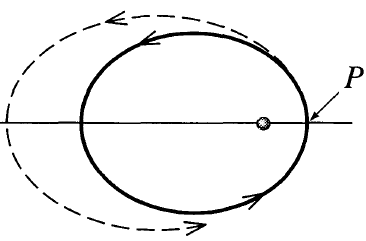
\includegraphics[width=0.85\textwidth]{Planetbevaegelse/Forward_thrust.png}
		\caption{Positivt boost således, at hastigheden øges, hvilket resulterer i et baneskift udad.}
		\label{fig:Forward_thrust}
	\end{subfigure}
	\hspace{5mm}
	\begin{subfigure}{0.45\textwidth}
		\centering
		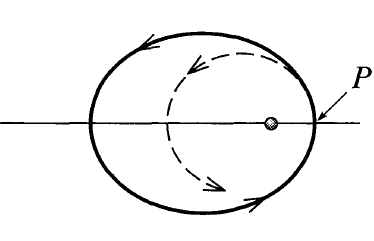
\includegraphics[width=0.85\textwidth]{Planetbevaegelse/Backward_thrust.png}
		\caption{Negativt boost således, at hastigheden sænkes, hvorved der foretages et baneskift indad.}
		\label{fig:Backward_thrust}
	\end{subfigure}
	\caption{Et objekts oprindelige bane er angivet med en streg, mens dets nye bane efter baneskift er vist med en stiplet linje. Baneskiftet foretages her i punktet $P$, hvilket kaldes periapsis, hvor punktet, der ligger lige modsat $P$ på den vandrette akse, kaldes apoapsis. (Kilde: \textit{Classical Mechanics}, John R. Taylor, figur 8.12.)}
	\label{fig:Boost_Forward_Backward}
\end{figure}

Først skal det lige fastsættes, hvad der menes med periapsis. Periapsis er det punkt på en bane, hvor der er mindst afstand mellem de to indgående objekter, hvilket i figur \ref{fig:Boost_Forward_Backward} er angivet med et $P$. Ligeledes findes et navn for det punkt på en bane, hvor der er størst afstand mellem de to indgående objekter, hvilket er apoapsis, og denne kan på figur \ref{fig:Boost_Forward_Backward} ses som liggende lige modsat $P$ på den vandrette akse.\footnote{Periapsis og apoapsis er de generelle betegnelser for disse punkter. For bestemte andre situationer findes også andre navne for disse punkter: For en bane omkring Solen benævnes periapsis og apoapsis henholdsvis perihelium og aphelium, og for en bane omkring Jorden benævnes disse henholdsvis perigæum og apogæum.}

\noindent
Scenariet, som betragtes nu, er en satellit, der foretager et baneskift, ved at affyre sine raketter enten fremad eller bagud tangentielt til dens bane, idet den befinder sig i periapsis, $\phi_0$. Koordinatsystemet for dette vælges således, at dets $x$-akse går gennem periapsis, hvor afstanden mellem Jorden og satellitten skal være kortest. Dette sker når argumentet til cosinus, $\phi_0-\delta_1$, er nul, da $\cos(0)=1$. Idet det vides, at $\phi_0$ er, når satellitten befinder sig i periapsis, og koordinatsystemets $x$-akse går gennem periapsis, da vil $\phi_0 = 0$, hvorfor $\delta_1 = 0$. Grundet at raketterne affyres i den tangentelle retning, vil satellittens retning ikke ændre sig under boostet, hvorfor den nye bane også vil have periapsis\footnote{Det er også muligt, at dette punkt kan være apoapsis, hvilket vil vise sig til sidst i afsnittet, så den mest præcise beskrivelse her ville være at sige, at den nye bane vil have apsis (et af yderpunkterne) i første banes periapsis, hvorfor $\delta = 0 \vee \delta = \pi$, men forskellen på disse er, om $\cos(\phi_0-\delta) = 1 \vee \cos(\phi_0-\delta) = -1$.} i $\phi_0$, og det derfor også må gælde, at $\delta_2 = 0$. På denne måde kan ligning \eqref{eq:r1(phi0)=r2(phi0)} reduceres til
\begin{align} \label{eq:Reduceret_r1(phi0)=r2(phi0)}
	\frac{c_1}{1+\epsilon_1} &= \frac{c_2}{1+\epsilon_2} \: .
\end{align}

\noindent
Der inføres nu en boostfaktor $\lambda$, som er svarende til forholdet mellem hastigheden efter, $v_2$, og før boostet, $v_1$,
\begin{align} \label{eq:Baneskift_boostfaktor}
	\lambda &= \frac{v_2}{v_1} \: .
\end{align}
Idet $\lambda > 1$ vil boostet være fremadrettet (positivt), da $v_2 > v_1$. For $0 < \lambda < 1$ vil boostet være tilbagerettet (negativt), da $v_2 < v_1$.

\noindent
Der laves nu to antagelser: For det første antages det, at satelittens masseændring grundet boostet er så lille, at den er negligibel, således at den reducerede masse $\mu$ er konstant før og efter boostet. For det andet antages det, at boostet foregår øjeblikkeligt, hvorfor satelitten er i samme punkt, $\phi_0$, før og efter boostet. Ud fra dette, og med viden om, at impulsmomentet er proportionelt med hastigheden, vil følgende gøre sig gældende:
\begin{align}
	\ell_2 &= \lambda \ell_1 \: ,
\end{align}
og da $c$ er proportional med $\ell^2$ fås følgende:
\begin{align} \label{eq:Baneskift_c2}
	c_2 &= \lambda^2 c_1 \: .
\end{align}
Indsættes dette i ligning \eqref{eq:Reduceret_r1(phi0)=r2(phi0)} og isoleres excentriciteten af bane 2, $\epsilon_2$, fås
\begin{align} \label{eq:Baneskift_epsilon2}
	\epsilon_2 &= \lambda^2\epsilon_1+(\lambda^2-1) \: .
\end{align}
%
Fra ligning \eqref{eq:Baneskift_epsilon2} kan det ses, at boostes satelitten positivt, $\lambda > 1$, vil den nye bane have en excentricetet større end den første bane, $\epsilon_2 > \epsilon_1$. De to baner vil altså have samme periapsis, men satelitten vil i den nye bane komme længere væk fra Jorden, se figur \ref{fig:Forward_thrust}. Ved en stor nok $\lambda$ vil excentriciteten af den nye bane blive større end $1$, hvilket er svarende til en hyperbolsk bane, hvilken er åben, hvorfor satellitten kan undslippe fra Jorden. \\
Hvis i stedet satellitten boostes negativt, således at $\lambda < 1$, vil den nye banes excentricitet være mindre end den første banes, $\epsilon_2 < \epsilon_1$, hvorfor den nye bane vil ligge indenfor den første bane, men de to baner vil stadig have samme periapsis. \\
Mindskes $\lambda$ nås et punkt, hvor $\epsilon_2 = 0$, og her kommer satelitten i en cirkulær bane omkring Jorden. Mindskes $\lambda$ fortsat opnås en negativ excentricitet, hvilket giver fin mening, når det indsættes i formlen for afstanden mellem to objekter, hvor det ene er i banebevægelse om det andet, ligning \eqref{eq:Generel_formel_r(phi)}, der så ser ud på følgende måde
\begin{align}
	r(\phi) &= \frac{c}{1-\epsilon\cos(\phi)} \: ,
\end{align}
hvilket er svarende til afstanden fra Jorden og til apoapsis, hvorfor periapsis i den første bane i dette tilfælde vil sammenfalde med apoapsis.
\chapter{Geometrisk Optik} \label{cha:Optik}

\section{Introduktion}
I geometrisk optik bruger man en simpel model for lys, hvor lyset beskrives som stråler, der bevæger sig i lige linjer. Denne model siger ikke noget om den præcise natur af lyset, men sammen med nogle få love er den tilstrækkelig til at give en beskrivelse af både refleksion og refraktion (brydning) af lys. På figur \ref{ind_ud_og_obj_img_def} del A) er der vist et eksempel på en indgående lysstråle, der reflekteres og brydes ved en overflade mellem to materialer. Der er også tegnet en stiplet linje på figuren, som er vinkelret på overfladen. En sådan linje kaldes for overfladens normal, og den bruges som en reference til at måle indgangsvinklen $\theta_a$, refleksionsvinklen $\theta_r$ og brydningsvinklen $\theta_b$, der også er vist på figuren. Disse processer er beskrevet ved de følgende to love.\\

\noindent
\textbf{Refleksionsloven}: Denne lov siger, at når en lysstråle reflekteres ved en overflade, så vil indgangsvinklen være lig refleksionsvinklen:
\begin{equation}
\theta_a = \theta_r
\end{equation}
\textbf{Brydningsloven}: Denne lov siger, at når en lysstråle brydes ved overgangen mellem to forskellige materialer $a$ og $b$, så er forholdet mellem indgangsvinklen og brydningsvinklen beskrevet ved den følgende formel\footnote{Nogle gange kaldes denne lov også for Snells Lov.}:
\begin{equation}
n_a \sin(\theta_a) = n_b \sin(\theta_b) 
\label{bryd_lov}
\end{equation}
Her er $n_a$ og $n_b$ brydningsindekserne for de to materialer. Brydningsindekset for et materiale er defineret som
\begin{equation}
n = \frac{c}{v},
\end{equation}
hvor $c$ er lysets fart i vakuum, og $v$ er lysets fart i materialet. I en mere komplet model, hvor lyset beskrives som elektromagnetiske bølger, kan man udlede begge disse love, men her vil de blot blive betragtet som eksperimentelle resultater.\\

Udover disse to love og vores simple model for lyset, er der to andre koncepter, som er helt centrale for geometrisk optik. Det første er konceptet om et \textit{objekt}, hvilket her defineres som enhver form for genstand, der kan udsende eller reflektere lys. Det andet er konceptet om et \textit{billede}, der er den reflekterede eller brudte version af objektet, som en observatør rent faktisk ser. Der er vist et eksempel på figur \ref{ind_ud_og_obj_img_def} del B), som illustrerer de to koncepter.
\begin{figure}[h!]
	\centering
	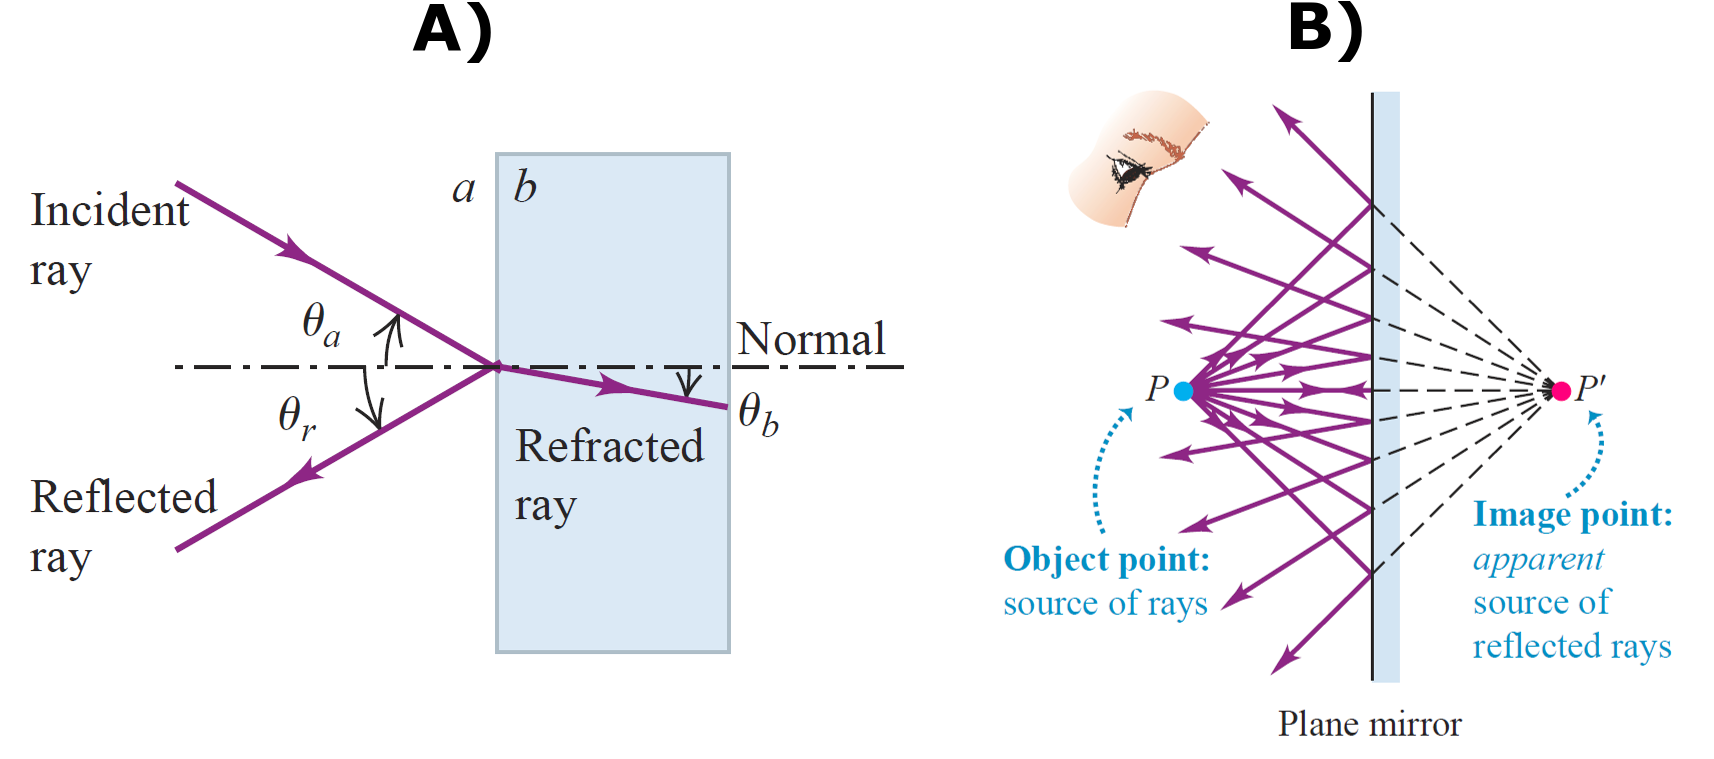
\includegraphics[scale=0.22]{Geometrisk-Optik/ind_ud_og_obj_img_def.PNG}
	\caption{På figurens del A) ses en indkommende lysstråle, der reflekteres og brydes ved overgangen mellem to materialer $a$ og $b$. På del B) ses et punktobjekt placeret i punktet $P$ og objektets billede i punktet $P'$, der er dannet af spejlet. Billedpunktet $P'$ er som illustreret det punkt, hvor observatøren ser objektet være.}
	\label{ind_ud_og_obj_img_def}
\end{figure}

\section{Billeddannelse}

\subsection*{Billeddannelse ved Fladt Spejl}

Som et første eksempel på billeddannelse betragtes et simpelt punktobjekt (et objekt uden en fysisk udstrækning), der placeres i nærheden af et fladt spejl, som det er vist på figur \ref{billeddannelse_flad_og_pil} del A). Her er $s$ afstanden mellem objektet og spejlet, der kaldes for objektafstanden, mens $s'$ er afstanden mellem billedet og spejlet, der kaldes billedafstanden. Derudover er der de to punkter, $P$ og $P'$, der angiver placeringen af objektet og billedet, og som derfor kaldes for henholdsvis objekt- og billedpunktet. På figuren er der også vist et eksempel på en lysstråle, der danner en vinkel $\theta$ i forhold til overfladens normal (stiplede linje). Det centrale at bemærke her er, at man lige så godt kunne have valgt en hvilken som helts anden vinkel $\theta'$, og man ville stadig have det samme billedpunkt.\\  

Når man skal arbejde med objekt- og billedafstandene, $s$ og $s'$, er der nogle fortegnskonventioner, som man skal huske at følge. Disse er givet ved de første 2 af de følgende regler. Den 3. regel er ikke relevant for eksemplet her med et fladt spejl, men den bliver vigtig, når man skal arbejde med refleksion og brydning ved krumme overflader. De 3 regler er som følger:\\

\noindent
1. \textbf{Regl for objektafstand:} Når et objekt er på samme side af den reflekterende eller brydende overflade som den indkommende lysstråle, er objektafstanden $s$ positiv. Ellers er den negativ.\\

\noindent
2. \textbf{Regl for billedafstand:} Når et billede er på samme side af den reflekterende eller brydende overflade som den udgåede lysstråle, er billedafstanden $s'$ positiv. Ellers er den negativ.\\

\noindent
3. \textbf{Regl for krumningsradius af en sfærisk overflade:} Når krumningscentrummet $C$ er på samme side som den udgående lysstråle, er krumningsradiusen $r$ positiv. Ellers er den negativ.\\

Kigger man igen på eksemplet med et fladt spejl, ser man hurtigt, at objektet altid vil være på samme side som den indgående lysstråle, og at billedet altid vil ligge på den anden side af den udgående lysstråle. Derfor kan man for et fladt spejl give følgende resultat:
\begin{equation}
s = -s' \quad \quad \quad \left( \text{for fladt spejl} \right)
\label{obj_img_fladt}
\end{equation}

\begin{figure}[h!]
	\centering
	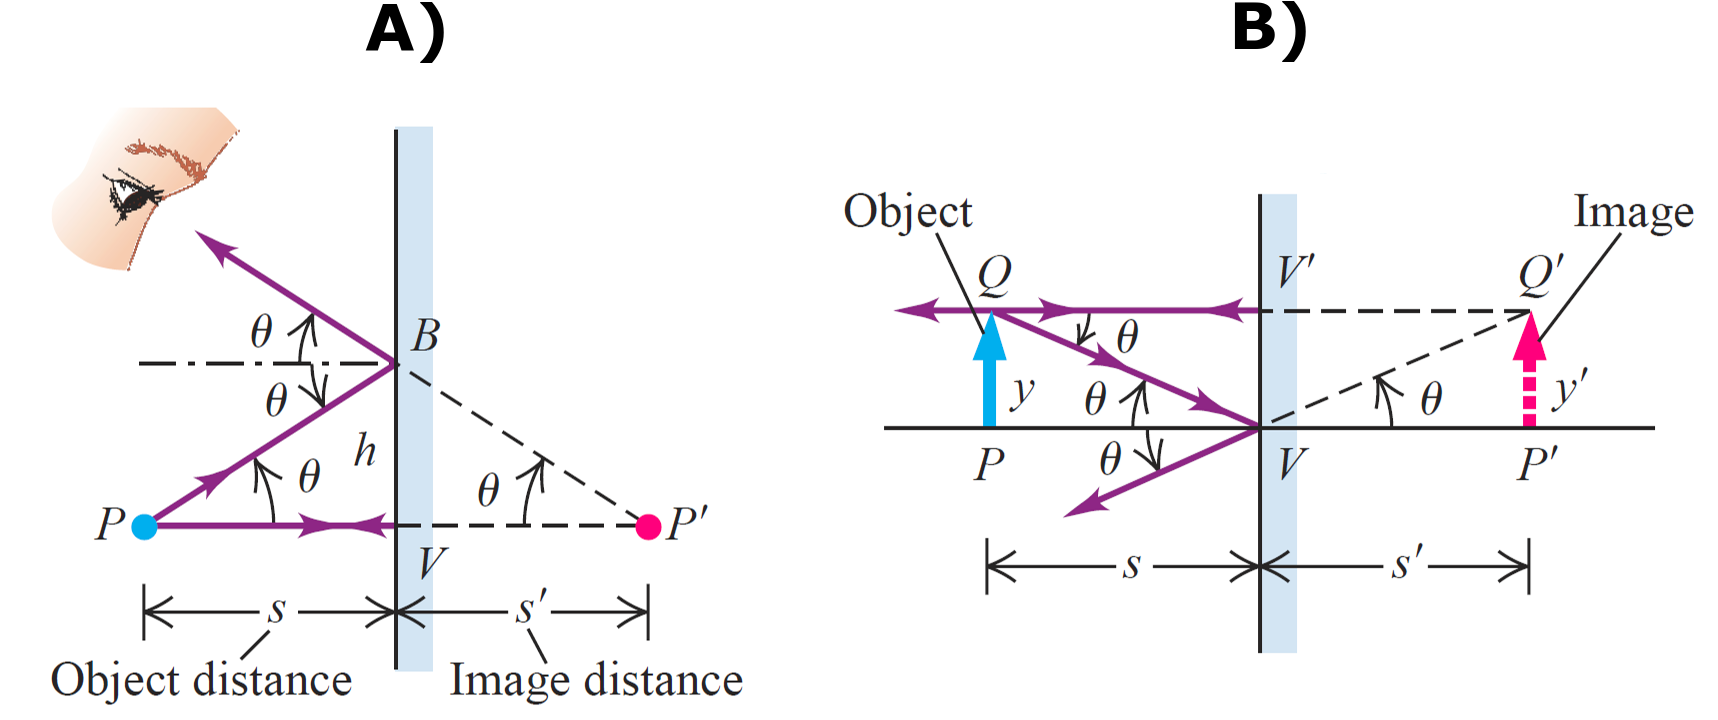
\includegraphics[scale=0.23]{Geometrisk-Optik/billeddannelse_flad_og_pil.PNG}
	\caption{På figurens del A) ses et punktobjekt og billedobjekt ved et fladt spejl samt objektafstanden $s$ og billedafstanden $s'$. På del B) ses en pil i blå der udgør objektet, som her har en udstrækning, mens billedet af objektet er angivet med den lyserøde pil, der også har en udstrækning. Også her er der angivet objekt- og billedafstand.}
	\label{billeddannelse_flad_og_pil}
\end{figure}
Selvom dette simple eksempel giver en god illustration af nogle af de grundlæggende begreber i geometrisk optik, er det ikke et særligt realistisk eller relevante eksempel, da punktobjekter ikke findes ude i naturen. Det er derfor oplagt at kigge på et lidt mere generelt tilfælde, hvor objektet har en fysisk udstrækning. Et eksempel på dette kan være en pil med en given længde $y$, som det er vist i figur \ref{billeddannelse_flad_og_pil} del B). Her ses det, at når man har et objekt med en udstrækning $y$, så får man også et billede med en udstrækning $y'$. I dette eksempel består objektet af alle punkter på linjen $PQ$, mens billedet består af alle punkter på linjen $P'Q'$. Kigger man på et enkelt punkt af objektet, f.eks $Q$, ser man også, at dette punkt svarer til et enkelt punkt af billedet, hvor det her er $Q'$. Altså vil en observatør, på samme side af spejlet som den indgående lysstråle, se pilespidsen ligge i punktet $Q'$ og ikke $Q$. En vigtig ting her er, at ligesom med $s$ og $s'$, så er der også en fortegnskonvention for størrelserne $y$ og $y'$. Denne konvention siger blot, at hvis objekt- og billedpilen peger i samme retning, så er $y$ og $y'$ positive, mens hvis objekt- og billedpilen peger i modsatte retninger, så er $y$ positiv og $y'$ er negativ.\\

Når man arbejder med objekter og billeder, der har en udstrækning, definerer man typisk en tværgående forstørrelse $m$ som forholdet mellem højden af billedet og objektet på følgende måde:
\begin{equation}
m = \frac{y'}{y}
\end{equation}
Benytter man fortegnskonventionen for $y$ og $y'$, ses det, at hvis objekt- og billedpilen peger i samme retning, så er $m$ positiv, og hvis de peger i modsatte retninger er $m$ negativ. Kigger man igen på figur \ref{billeddannelse_flad_og_pil} del B), kan man se, at objekt- og billedpilen altid vil pege i samme retning for et fladt spejl, og at $y$ og $y'$ vil være lige store. Dette giver altså følgende resultat
\begin{equation}
m = +1 \quad \quad \quad \left( \text{for fladt spejl} \right)
\end{equation}
Som det ses i de to gennemgåede eksempler ovenover, er det muligt at danne billeder af både punktobjekter og objekter med udstrækning ved et fladt spejl. Det er dog begrænset, hvor anvendeligt dette er, da man ikke kan variere den tværgående forstørrelse $m$, hvilket er essentielt, hvis man vil bruge geometrisk optik, til at lave forskellige teknologier som mikroskoper eller teleskoper. For at opnå denne frihed til at variere $m$, må man gå væk fra det simple tilfælde med et fladt spejl, og i stedet kigge på refleksion og brydning ved krumme overflader.  

\subsection*{Billeddannelse ved Krumme Overflader}

Det næste man kan kigge på indenfor geometrisk optik er, hvad der sker, hvis man skifter det flade spejl ud med et spejl med en krum overflade. Som et første eksempel er det oplagt at kigge på et hulspejl, hvor spejlet består af et udsnit af en cirkel, som det er vist på figur \ref{billeddannelse_krum}. Her er $R$ cirklens radius, $C$ kaldes for krumningscentrummet og ligger i cirklens centrum, $V$, der ligger i spejlets centrum, kaldes for spejlets vertex og den vandrette streg langs $CV$ kaldes for den optiske akse. 
%
\begin{figure}[h!]
	\centering
	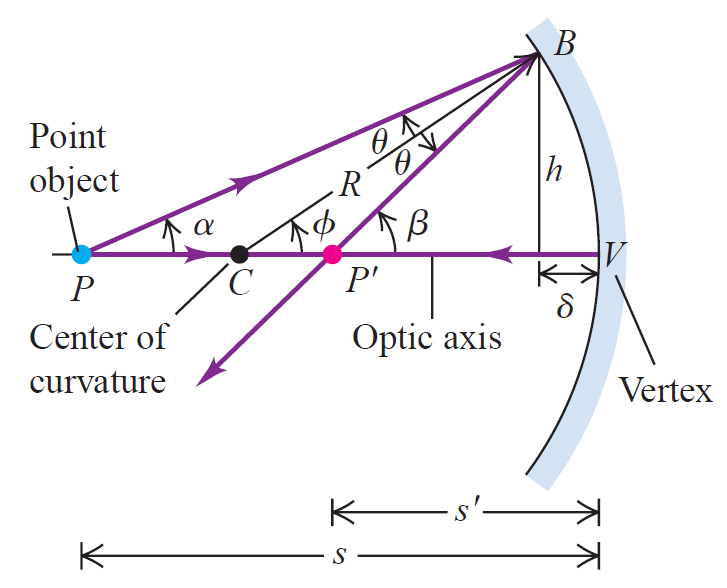
\includegraphics[scale=0.3]{Geometrisk-Optik/billeddannelse_krum.PNG}
	\caption{På figuren ses et punkobjekt placeret i punktet $P$ samt billedet af dette punktobjekt placeret i punktet $P'$ dannet ved et hulspejl.}
	\label{billeddannelse_krum}
\end{figure}
%
På samme måde som i \eqref{obj_img_fladt} vil man gerne finde en sammenhæng mellem objekt- og billedafstanden $s$ og $s'$. Dette kan gøres ved at lave nogle geometriske overvejelser ud fra figur \ref{billeddannelse_krum}. Kigger man først på trekanten $PBC$, ses det fra figuren at\footnote{Her angives vinklerne i radianer. Man finder en vinkel i radianer ud fra vinklen i grader ud fra formlen: $v_{\text{rad}} =  \pi \cdot \left( v_{\text{grad}} /180 \degree \right)$}
$$\pi = \alpha + \theta + x \, ,$$
hvor $x$ er den stumpe vinkel ved krumningscentrummet $C$. Dette siger blot, at alle tre vinkler i trekanten $PBC$ summer op til $\pi$ radianer (altså 180 grader). Man kan da bemærke, at vinklen $x$ i trekant $PBC$ og vinklen $\phi$ i trekant $CBP'$ til sammen udspænder $\pi$ radianer. Det betyder at
$$\pi = x + \phi \qquad \Rightarrow \qquad x = \pi - \phi$$
Sætter man dette ind i den ovenstående ligning, finder man da at
$$\phi = \alpha + \theta$$
På samme måde kan man kigge på trekanten $CBP'$, hvor man ved lignende overvejelser finder at
$$\beta = \phi + \theta$$
Ud fra disse to resultater kan man løse to ligninger med fire ubekendte, hvilket giver en ligning der relaterer $\alpha$, $\beta$ og $\phi$
\begin{equation}
\alpha + \beta = 2 \phi
\label{a_b_phi}
\end{equation}
Husker man da på fortegnskonventionerne fra det forrige afsnit, ses det, at både $s$, $s'$ og $R$ er positive størrelser. Ideen er da, at kigge på tangens til vinklerne $\alpha$, $\beta$ og $\phi$, og at udtrykke disse vha. størrelserne fra figur \ref{billeddannelse_krum}. Husker man, at tangens til en vinkel i en retvinklet trekant, forskellig fra den rette vinkel, kan skrives som den modstående divideret med den hosliggende katete, finder man at
$$\tan \alpha = \frac{h}{s - \delta}, \quad \quad \tan \beta = \frac{h}{s' - \delta}, \quad \quad \tan \phi = \frac{h}{R - \delta}. $$
Disse tre ligninger er ikke lige til at løse, men hvis man antager, at vinklen $\alpha$ er lille, således at $\beta$ og $\phi$ også er små, kan man lave en approksimation af tangens. Rent fysisk svarer dette til tilfældet, hvor objektafstanden $s$ er meget større end højden af spejlet $h$. I forhold til approksimationen af tangens gælder det, at $\tan x \approx x$, hvis $x$ er lille og angivet i radianer. Det bemærkes videre, at $\delta$ også vil være lille i dette tilfælde, så den kan også ignoreres. Dette giver tre ligninger
$$\alpha = \frac{h}{s}, \quad \quad \beta = \frac{h}{s'}, \quad \quad \phi = \frac{h}{R}.$$
Sætter man dette ind i relationen \eqref{a_b_phi}, får man da at
\begin{equation}
\frac{1}{s} + \frac{1}{s'} = \frac{2}{R}
\label{obj_img_krum}
\end{equation}
Som det næste er det interessant at kigge på, hvad der sker, hvis man tager objektet og flytter det uendeligt (i praksis meget) langt væk fra spejlet. Fysisk vil dette betyde, at alle de indgående stråler bevæger sig parallelt med den optiske akse, som illustreret på figur \ref{focal_point_12} del A). I dette tilfælde vil $1/s = 0$, hvilket ifølge \eqref{obj_img_krum} må give at
$$\frac{1}{s'} = \frac{2}{R} \quad \quad \Rightarrow \quad \quad s' = \frac{R}{2}$$
Det viser, at alle indkommende stråler vil have den samme billedafstand $s'$, og altså vil alle de indgående stråler samle sig i et enkelt punkt $F$, som det også er vist på figur \ref{focal_point_12} del A). Dette punkt kaldes for spejlets brændpunkt, og afstanden fra dette  til spejlets vertex kaldes for spejlets brændvidde, der betegnes $f$. Her har man, at brændvidden er givet ved
\begin{equation}
f = \frac{R}{2}
\label{focal_point_eq}
\end{equation} 
Som det ses af denne ligning afhænger brændvidden $f$ kun af $R$, hvilket betyder at både brændvidden $f$ og placeringen af brændpunktet $F$ er uafhængige af objekt- og billedafstanden $s$ og $s'$. brændpunkter er altså karakteristisk egenskab for et givet spejl.\\
Et andet interessant tilfælde, er det hvor objektet placeres i brændpunktet $F$, hvilket betyder at objektafstanden bliver $s = f = R/2$. Sætter man dette ind i \eqref{obj_img_krum} finder man således at
$$\frac{R}{2} + \frac{1}{s'} = \frac{R}{2} \quad \quad \Rightarrow \quad \quad \frac{1}{s'} = 0 \quad \quad \Rightarrow \quad \quad s' = \infty$$
Det viser, at billedet ligger uendeligt langt væk, således at alle de udgående lysstråler vil være parallelle med den optiske akse, som det er illustreret i figur \ref{focal_point_12} del B). Nu hvor brændvidden er blevet indført, er det mere konventionelt at skrive formel \eqref{obj_img_krum} på følgende form
\begin{equation}
\frac{1}{s} + \frac{1}{s'} = \frac{1}{f}
\label{ny_focal_s_s'}
\end{equation}

\begin{figure}[h!]
	\centering
	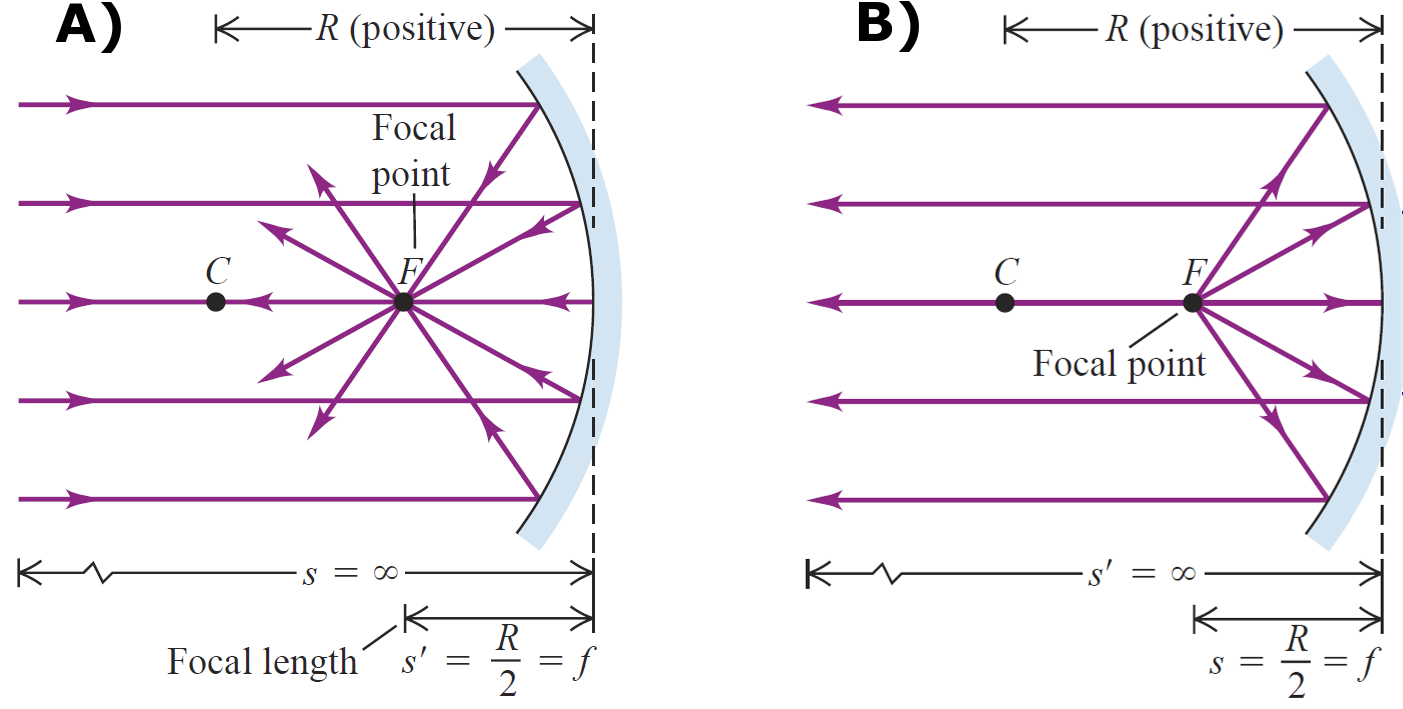
\includegraphics[scale=0.24]{Geometrisk-Optik/focal_point_12.PNG}
	\caption{På figurens del A) ses tilfældet hvor et objekt er placeret uendeligt langt fra et hulspejl, og hvor brændpunktet er placeret i punktet $F$. På del B) ses tilfældet, hvor objektet er placeret i brændpunktet $F$.}
	\label{focal_point_12}
\end{figure}
Det næste spørgsmål man kan stille sig selv er nu, hvad der sker, hvis man i stedet for et punktobjekt valgte et objekt med en udstrækning. Et eksempel på dette er vist på figur \ref{spejl_krum_pil}. Det vigtigste at bemærke her er, at man får to ensvinklede trekanter $PQV$ og $P'Q'V$. Det betyder specielt, at forholdet mellem længden af siderne $PV$ og $P'V$, er det samme som for siderne $PQ$ og $P'Q'$. Fra dette får man således
\begin{equation}
m = \frac{y'}{y} = - \frac{s'}{s}
\end{equation}

\begin{figure}[h!]
	\centering
	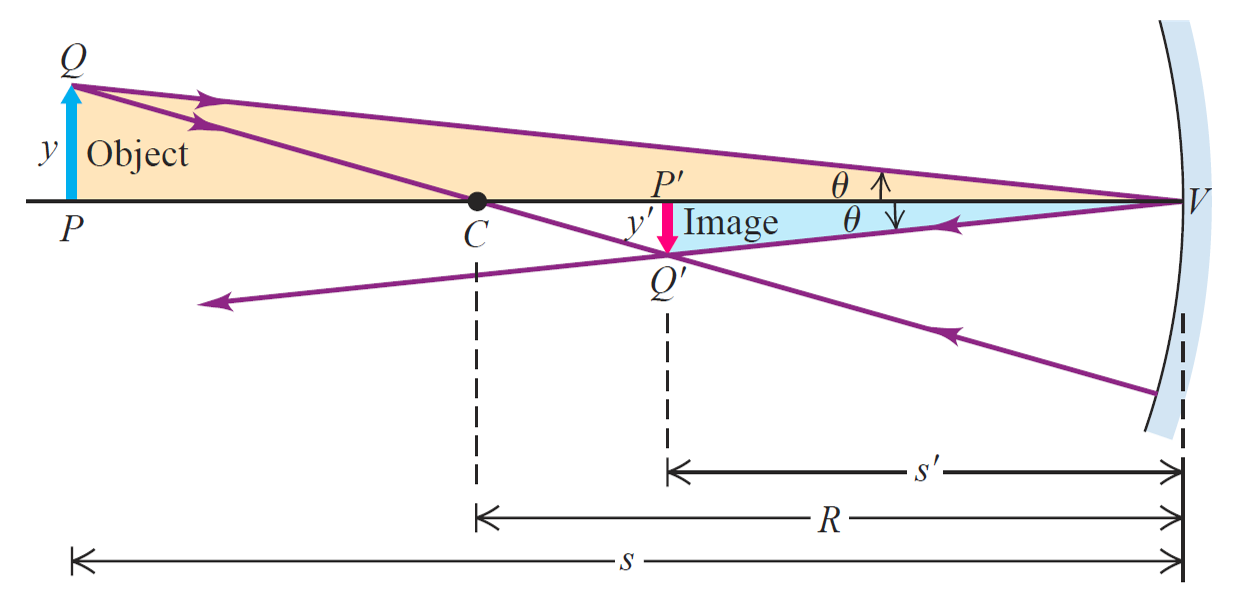
\includegraphics[scale=0.27]{Geometrisk-Optik/spejl_krum_pil.PNG}
	\caption{På figuren ses et eksempel på refleksion af et objekt med en udstrækning ved et hulspejl.}
	\label{spejl_krum_pil}
\end{figure} 
Nu hvor de fleste egenskaber ved refleksion fra et hulspejl er dækket, kan man kigge på hvad der sker, hvis man i stedet tager et såkaldt konvekst spejl, som er et spejl, der krummer væk fra observatoren i stedet for imod. To eksempler, hvor det ene er med et punktobjekt, og det andet er et objekt med en udstrækning, er vist på figur \ref{konveks_spejl}. På del A) af figuren kan man se, at krumningsradiusen $R$ her vil være negativ. Man kan da bruge den samme metode som for hulspejlet til at vise, at man her har relationen
\begin{equation}
\frac{1}{s} + \frac{1}{s'} = \frac{2}{R}
\end{equation}
På samme måde kan man også vise at
\begin{equation}
m = \frac{y'}{y} = - \frac{s'}{s}
\label{ref_for_jacob}
\end{equation}

\begin{figure}[h!]
	\centering
	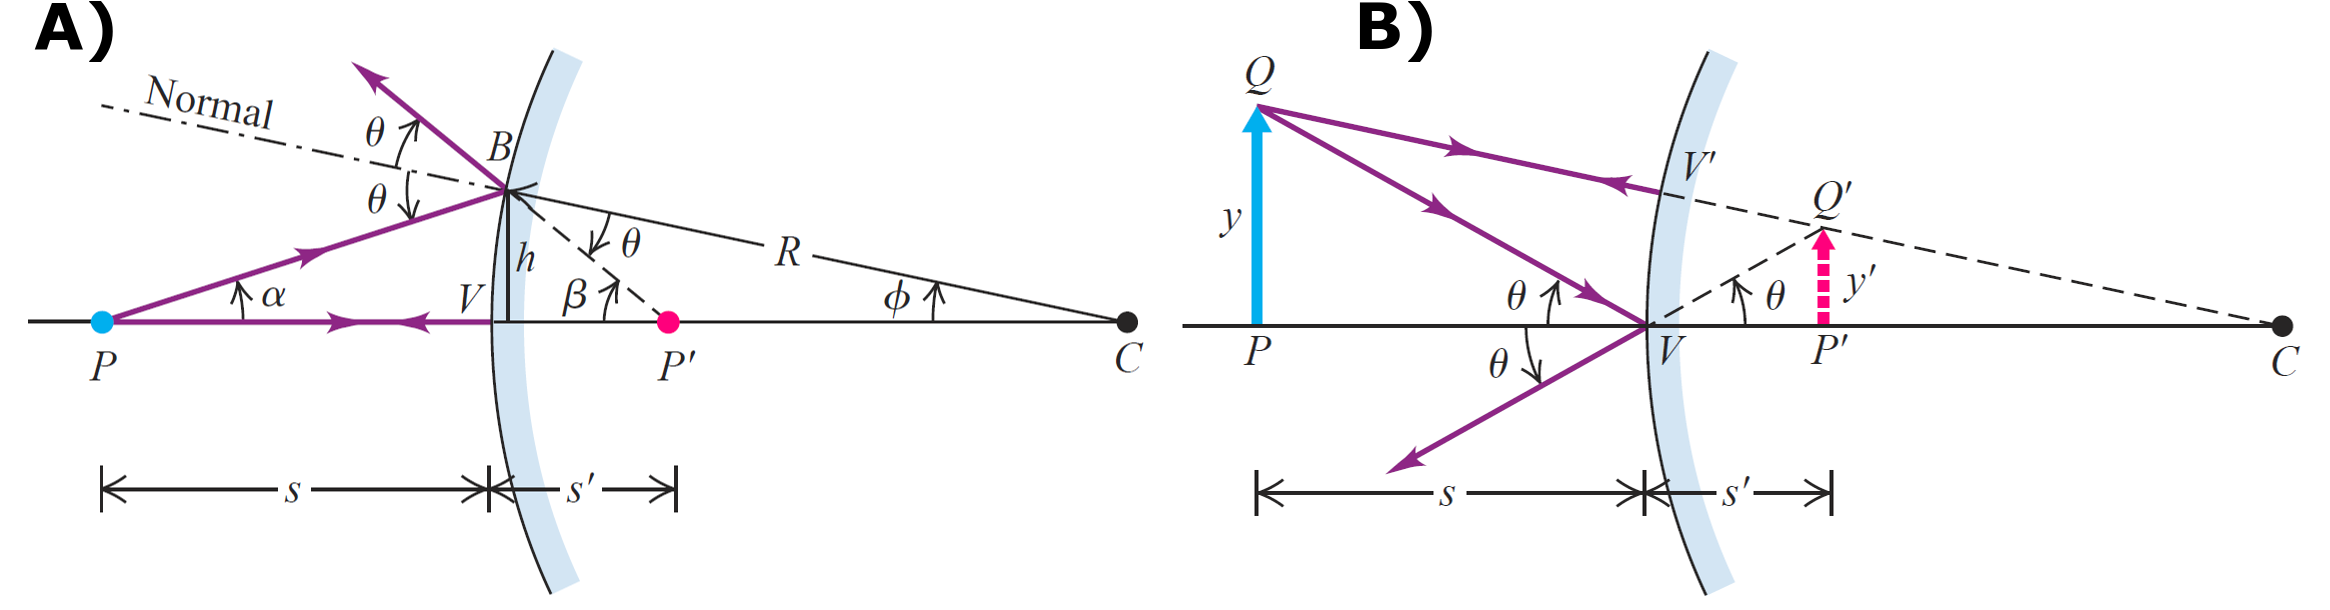
\includegraphics[scale=0.195]{Geometrisk-Optik/konveks_spejl.PNG}
	\caption{På figurens del A) ses et punktobjekt placeret i $P$, der ved refleksion ved et konvekst spejl danner billedet i $P'$. På del B) ses et objekt med en udstrækning, der også danner et billede ved refleksion.}
	\label{konveks_spejl}
\end{figure}
Ligesom for hulspejlet kan man også tale om brændpunkter og brændvidder for konvekse spejle. Kigger man på situationen i figur \ref{konveks_spejl2} del A), hvor de indkommende lysstråler er parallelle med den optiske akse, vil de ikke samle sig i et brændpunktet på samme måde, som det var tilfældet for hulspejlet. Til gengæld vil de udgående lysstråler se ud som om, at de kommer fra brændpunktet $F$ i en afstand $f$ bag spejlet. Her kalder man $f$ for brændvidden og $F$ for et virtuelt brændpunkt. Man finder også på samme vis som før at 
$$f = \frac{R}{2}$$
Den overordnede pointe er altså, at formlerne \eqref{spejl_krum_pil}, \eqref{obj_img_krum}, \eqref{focal_point_eq} og \eqref{ny_focal_s_s'} holder både for hulspejle og konvekse spejle, så længe man husker at bruge fortegnsreglerne for $s$, $s'$ og $R$ rigtigt.  
\begin{figure}[h!]
	\centering
	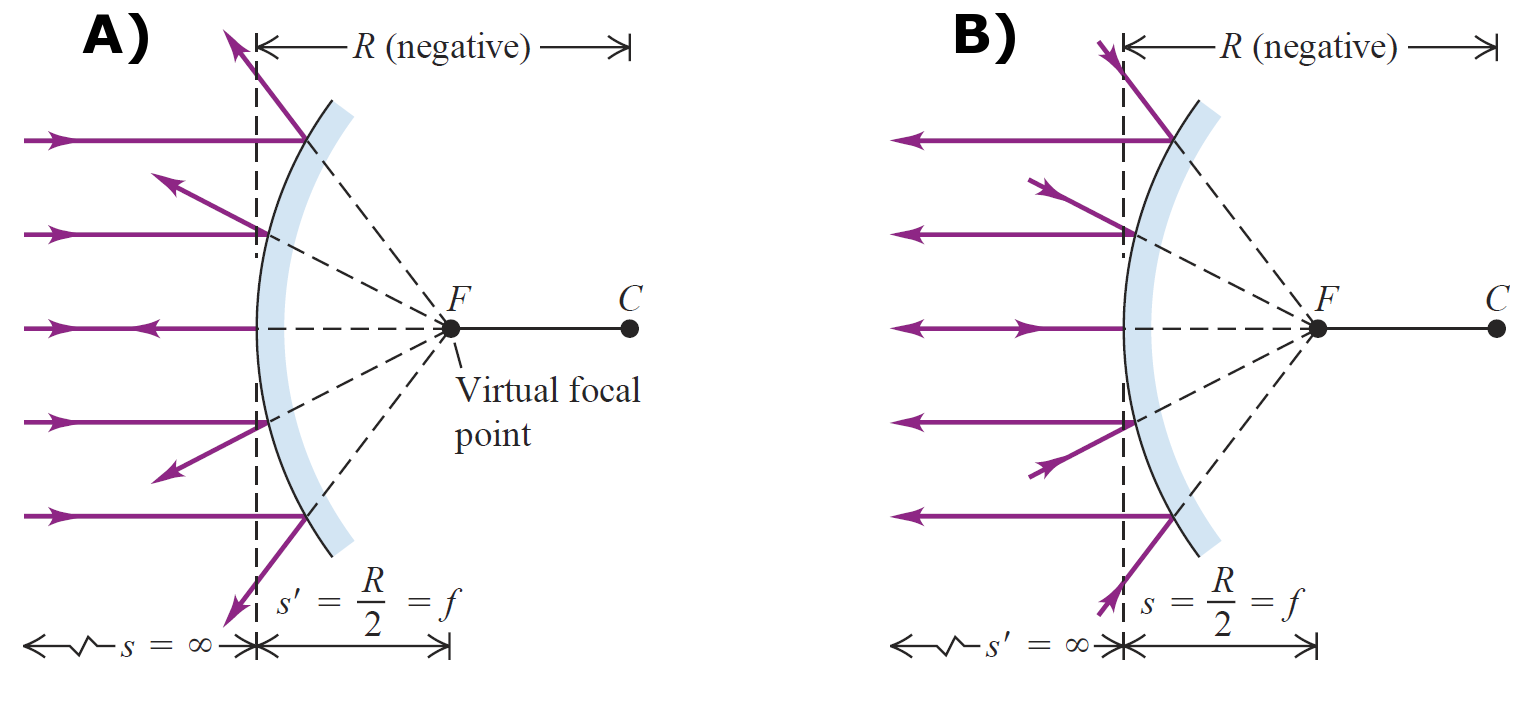
\includegraphics[scale=0.23]{Geometrisk-Optik/konveks_spejl2.PNG}
	\caption{På figurens del A) ses situationen, hvor objektet er placeret uendeligt langt væk fra spejlet. På del B) ses situationen, hvor objektet er placeret i det virtuelle brændpunkt $F$.}
	\label{konveks_spejl2}
\end{figure}
Før man går videre og kigger på, hvordan man kan bruge geometrisk optik til at beskrive linser, er det værd først at kigge på billeddannelse ved brydning for en krum overflade i stedet for ved refleksion, som det er gjort indtil nu. Et eksempel på dette, med et punktobjekt, er givet i figur \ref{konveks_brydning}. Det første man gerne vil, er at finde relationen mellem objekt- og billedafstanden. Dette kan igen gøres ved at lave nogle geometriske overvejelser. Kigger man først på trekanterne $PBC$ og $P'BC$, finder man at
$$\theta_a = \alpha + \phi \quad \quad \quad \quad \phi = \beta + \theta_b$$
Det næste man kan gøre, er da at bruge formel \eqref{bryd_lov} sammen med tangens til vinklerne $\alpha$, $\beta$ og $\phi$. Dette giver følgende udtryk
$$n_a \sin \theta_a = n_b \sin \theta_b \quad \quad \tan \alpha = \frac{h}{s + \delta} \quad \quad \tan \beta = \frac{h}{s' + \delta} \quad \quad \tan \phi = \frac{h}{R - \delta}$$
Det næste trin herfra er at antage, at $\alpha$ er lille, da det vil betyde, at alle de andre vinkler også er små. Derfor kan man lave en approksimation af både sinus og tangens til de forskellige vinkler, og bruge at $\delta$ bliver lille i forhold til $s$ og $s'$, så den også kan ignoreres. Det giver
$$n_a \theta_a = n_b \theta_b \, , \quad \quad \alpha = \frac{h}{s} \, , \quad \quad \beta = \frac{h}{s'} \, , \quad \quad \phi = \frac{h}{R} \, . $$
Bruger man udtrykket for $\theta_a$ fra før finder man da at
$$ \theta_b = \frac{n_a}{n_b} \left( \alpha + \phi \right) \, ,$$
og man kan da sætte det ind i udtrykket for $\phi$ fra før og få
$$\phi = \beta +  \frac{n_a}{n_b} \left( \alpha + \phi \right) \quad \quad \Rightarrow \quad \quad n_a\alpha + n_b \beta = \phi \left( n_b - n_a \right)$$
Endeligt kan man sætte de nye udtryk for $\alpha$, $\beta$ og $\phi$ ind i denne formel, hvilket giver det endelige resultat
\begin{equation}
\frac{n_a}{s} + \frac{n_b}{s'} = \frac{n_b - n_a}{R} 
\label{ref_til_jacob2}
\end{equation}
\begin{figure}[h!]
	\centering
	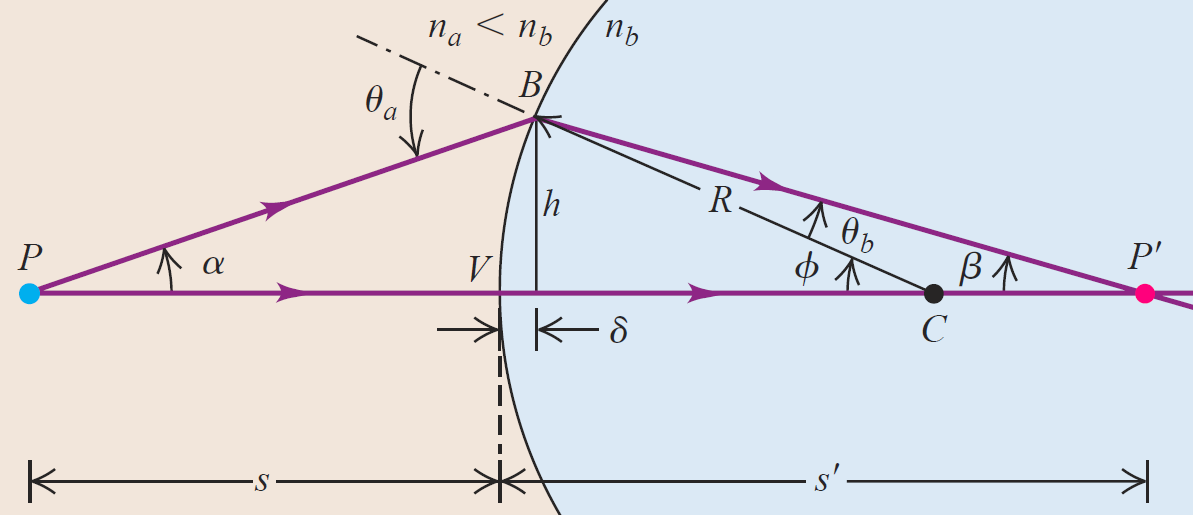
\includegraphics[scale=0.27]{Geometrisk-Optik/konveks_brydning.PNG}
	\caption{Figuren viser et eksempel på billeddannelse af et punktobjekt ved et konvekst spejl.}
	\label{konveks_brydning}
\end{figure}

Det sidste man gerne vil finde er forstørrelsen, når man har et objekt med en udstrækning. Dette gøres ved at betragte opsætningen på figur \ref{konveks_brydning2}. Det første man kan bemærke er, at man for trekanterne $PQV$ og $P'Q'V$ får
$$\tan \theta_a = \frac{y}{s} \, , \quad \quad \quad \quad \tan \theta_b = - \frac{y'}{s'} \, .$$
Fra \eqref{bryd_lov} får man også at
$$n_a \sin \theta_a = n_b \sin \theta_b$$
Så bruges det, at man for små vinkler har, at $\sin \theta \approx \tan \theta$, så man samlet set får at
$$\frac{n_a y}{s} = - \frac{n_b y'}{s'} \, ,$$
eller efter en lille omskrivning
\begin{equation}
m = \frac{y'}{y} = - \frac{n_a s'}{n_b s}
\end{equation}

\begin{figure}[h!]
	\centering
	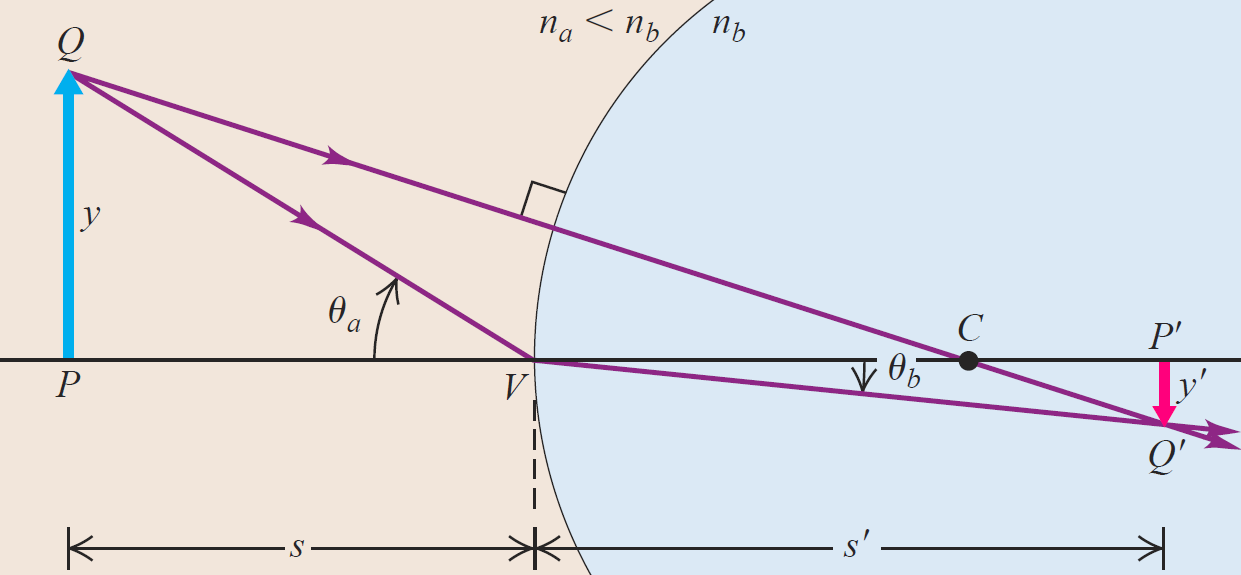
\includegraphics[scale=0.26]{Geometrisk-Optik/konveks_brydning2.PNG}
	\caption{Figuren viser et eksempel på billeddannelse af et objekt med en udstrækning ved et konvekst spejl.}
	\label{konveks_brydning2}
\end{figure} 

\section{Linser}
Vi vil i dette kapitel kigge nærmere på et af de mest brugte optiske værktøjer (efter det flade spejl), den tynde linse. Tynde linser bliver brugt i et utal af forskellige forsøgsopstillinger, så som optik, laser fysik og astronomi, og er derfor yderst interessante at undersøge

\subsection{Tynde linser}

En linse er et optisk system bestående af to brydende overflader, hvor den tynde linse består af to sfæriske overflader tæt nok på hinanden til, at afstanden imellem dem er negligerbar. I dette afsnit vil der blive gjort brug af resultaterne fra forrige afsnit omkring brydning ved sfæriske overflader. Der bruges herudover samme fortegnsregler som defineret tidligere. \\

\begin{wrapfigure}{r}{6cm}
	\centering
	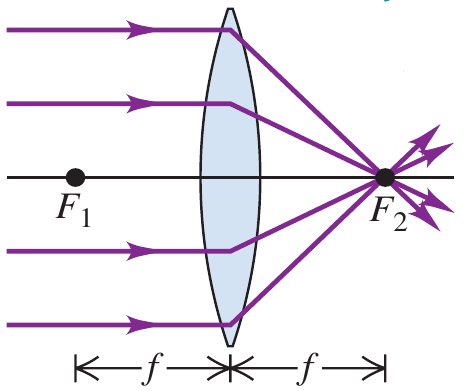
\includegraphics[width=4.5cm]{Geometrisk-Optik/conv_lens.PNG}
	\caption{Konvergerende tynd linse med brændpunkter $F_1$, $F_2$ og brændvidde $f$. } \label{fig:konv}
\end{wrapfigure}

\noindent En linse af formen vist i figur \ref{fig:konv} har den egenskab, at når stråler parallel til den optiske akse passerer igennem linsen, dannes der et billede ved punktet $F_2$. Omvendt, så vil stråler udsendt fra $F_1$ være parallelle til aksen efter at have passeret igennem linsen. Denne type af linse kaldes for en konvergerende linse. Punkterne $F_1$ og $F_2$ kaldes for hhv. det første og andet brændpunkt, mens afstanden $f$ (målt fra centrum af linsen) kaldes for brændvidden. For en konvergerende linse er brændvidden $f$ positiv. Bemærk her ligheden med det krumme spejl fra forrige kapitel. \\ 

\noindent Ligesom ved det krumme spejl, kan et konvergerende spejl danne et billede af et udstrakt objekt. Lad $s$ og $s'$ betegne hhv. objekt- og billedeafstanden og $y$ og $y'$ betegne hhv. objekt- og billedehøjden. På figur \ref{bla} ses strålen $QA$ brydes igennem $F_2$, mens strålen $QO$ passerer igennem uden at ændre retning, da vi har antaget at vi arbejder med en tynd linse, hvor overfladerne i centrum er parallelle. Vinklerne $\alpha$ er her ens, og derved må forholdet mellem siderne i trekanterne $PQO$ og $P'Q'O$ også være det,
\begin{equation}
\frac{y}{s} = -\frac{y'}{s'} \quad \text{eller} \quad \frac{y'}{y} = -\frac{s'}{s},
\label{eq:1}
\end{equation}

\noindent hvor det negative fortegn skyldes, at billedet er under den optiske akse. Vinklerne $\beta$ er også ens, hvilket medfører at forholdet mellem siderne i trekanterne $OAF_2$ og $P'Q'F_2$ også er ens, hvorved

\begin{equation}
\frac{y}{f}=-\frac{y'}{s'-f} \quad \text{eller} \quad \frac{y'}{y} = -\frac{s'-f}{f}
\label{eq:2}
\end{equation}

\noindent Ud fra ligning \eqref{eq:1} og ligning \eqref{eq:2} får vi relationen

\begin{equation}
\frac{1}{s}+\frac{1}{s'} = \frac{1}{f} \, ,
\label{eq:3}
\end{equation}

\noindent hvilket er den samme relation mellem objekt og billede, vi fandt for det konvekse spejl i ligning \eqref{ny_focal_s_s'}. Vi får herudover også et udtryk for den tværgående forstørrelse, ækvivalent til ligning \eqref{ref_for_jacob},

\begin{equation}
m = \frac{y'}{y} = -\frac{s'}{s}
\label{eq:4}
\end{equation}

\begin{figure}[h!]
	\centering
	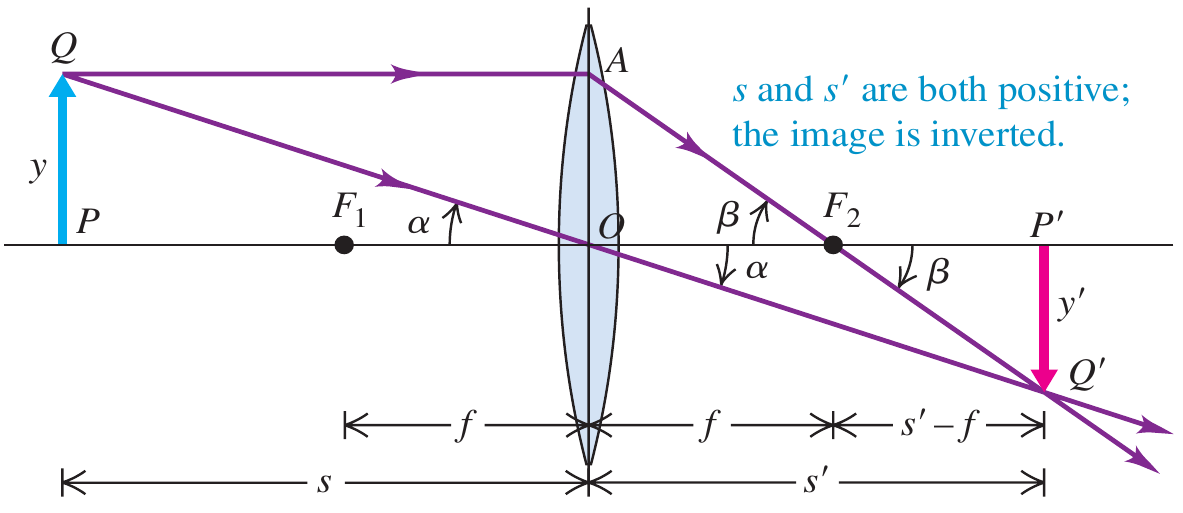
\includegraphics[scale=0.3]{Geometrisk-Optik/lens_objekt.PNG}
	\caption{Model til at finde objekt position for en tynd linse.}
	\label{bla}
\end{figure}

\noindent De to ovenstående ligninger er grundligningerne for tynde linser, og er som sagt af samme form som de tidligere fundne ligninger for sfæriske spejle. Det negative fortegn i ligning \eqref{eq:4} betyder, at når $s$ og $s'$ er positive, så vil billedet være inverteret , og $y$ og $y'$ vil have modsatte fortegn. Hvis vi antager at $f>0$ (en konvergerende linse), så giver ligning \eqref{eq:3} os, at når objektet er uden for det første brændpunkt $F_1$ ($s>f$) vil billedeafstanden $s'$ være positiv og billedet inverteret. Når billedeafstanden er positivt, er billedet per definition på den modsatte side af linsen end objektet, og kaldes for reelt. Omvendt så vil et objekt placeret inden for det første brændpunkt ($s<f$) danne et billede med negativ billedeafstand $s'$. Dette billede er ikke-inverteret, og placeret på samme side af linsen som objektet. Når billedeafstanden er negativ, og billedet befinder sig på samme side af linsen som objektet, kaldes billedet for virtuelt.

\newpage

\begin{wrapfigure}{r}{6cm}
	\centering
	\includegraphics[width=5cm]{Geometrisk-Optik/div_lens.PNG}
	\caption{Divergerende linse med negativ $f$, og brændpunkter $F_1$ og $F_2$.}
	\label{div}
\end{wrapfigure}

\noindent I figur \ref{div} vises en divergerende linse, en anden form for tynd linse. Lysstråler parallelle til den optiske akse divergere efter brydning. Brændvidden $f$ for divergerende linser er en negativ størrelse, mens brændpunkterne $F_1$ og $F_2$ er modsat placeret i forhold til den konvergerende linse. Parallelle stråler der brydes lader til at være udsendt fra punktet $F_2$, mens stråler der konvergerer mod punktet $F_1$ er parallelle til den optiske akse efter brydning, som set i hhv. figur \ref{div}a og figur \ref{div}b. Ud fra dette kan vi se at divergerende linser har det samme forhold til konvergerende linser, som konvekse spejle havde til konkave spejle i forrige kapitel. Man ville kunne foretage den samme geometriske analyse som tidligere i dette kapitel, for at vise at ligning \eqref{eq:3} og \eqref{eq:4} også er gældende for divergerende linser.\\

\subsection{Linsemagerens ligning}
\noindent Ud fra analysen af tynde linser påstår vi følgende, \\

\noindent \textsl{Enhver linse der er tykkere på midten end ved kanterne er en konvergerende linse, og enhver linser der er tykkere ved kanterne end på midten er en divergerende linse.} \\


\noindent Denne påstand kan vises ved at lave en dybdegående udledning af ligning \eqref{eq:3}, hvorved vi også vil udlede \textsl{Linsemagerens ligning}. Denne ligning beskriver forholdet mellem brændvidde $f$, linsens brydnings index $n$, og overfladernes radiusser $R_1$ og $R_2$. Vi starter generelt ud med en bi-konvergerende linse (bedre kendt som en bi-konveks linse) med tykkelse $t$ og med brydningsindeks $n_2$ omkredset af et materiale med brydningsindeks $n_1$, illustreret i figur \ref{bikonv}. De to sfæriske overflader har hhv. radiuserne $R_1$ og $R_2$. Vi betragter punktobjektet $P$, med objektafstand $s_1$ fra den første overflade. Lysstråler udsendt fra $P$ brydes af den første overflade og danner et virtuelt billede $Q'$ med billedeafstand $s'_1$. Ud fra de definerede fortegnskonventioner er $s_1>0$, $s_1'<0$ og $R_1>0$. Ud fra ligning \eqref{ref_til_jacob2} får man følgende relation,
\begin{equation}
\frac{n_1}{s_1}+\frac{n_2}{s'_1} = \frac{n_2-n_1}{R_1}
\label{eq:5}
\end{equation}

\noindent Det virtuelle billede $Q'$ danner nu et objekt med objektafstand $s_2 = \abs{s'_1}+t = t-s'_1$ for den anden sfæriske overflade. Stråler fra $Q'$ brydes og danner et reelt billede $Q$ med billedafstand $s'_2$. Her har vi at $s_2>0$, $s'_2>0$ og $R_2 < 0$. Vi kan da opstille relationen

\begin{equation}
\frac{n_2}{s_2}+\frac{n_1}{s'_2} = \frac{n_1}{s'_2} + \frac{n_2}{t-s'_1} = \frac{n_1-n_2}{R_2}
\label{eq:6}
\end{equation}

\begin{figure}[h!]
	\centering
	\includegraphics[scale=0.3]{Geometrisk-Optik/lensmaker.PNG}
	\caption{Brydning af lys igennem en bi-konveks linse med tykkelse $t$.}
	\label{bikonv}
\end{figure}


\noindent Ved at addere ligning \eqref{eq:5} og ligning \eqref{eq:6} får vi

\begin{equation}
\frac{n_1}{s_1}+\frac{n_2}{s'_1} + \frac{n_1}{s'_2} + \frac{n_2}{t-s'_1} = (n_2 - n_1) \left( \frac{1}{R_1} - \frac{1}{R_2} \right)
\end{equation}

\noindent For tynde linser er det gældende at $t\ll s'_1$, hvorved man får

\begin{equation}
\frac{1}{s_1}+\frac{1}{s'_2} = \left(\frac{n_2}{n_1}-1\right)\left( \frac{1}{R_1}-\frac{1}{R_2} \right)
\end{equation}

\noindent Her kan $s_1$ betragtes som objektafstanden $s$, $s'_2$ kan betragtes som billedeafstanden $s'$, og da vi oftest betragter linser i luft kan vi sætte $n_1=1$ og $n_2=n$, hvorved vi får følgende vha. ligning \eqref{eq:3}

\begin{equation}
\frac{1}{f} = \frac{1}{s} + \frac{1}{s'} = (n-1)\left( \frac{1}{R_1} - \frac{1}{R_2}\right)
\end{equation}

\noindent Den ovenstående ligning kaldes for Linsemagerens ligning, som er gældende for alle tynde linser. Ved brug af de definerede fortegnsregler, kan den tidligere påstand omkring konvergerende og divergerende linser vises, da linser der er bredere ved midten vil resultere i en positiv brændvidde, mens linser der er bredere ved enderne vil resultere i en negativ brændvidde. 






\appendix

%her skal matematik afsnittet sættes ind
\chapter{Matematik}
\label{cha:matematik}

I dette appendiks skal vi indføre nogle nyttige matematiske redskaber,
der er essentielle for fysikken. Selvom du måske kender noget af
matematikken i forvejen, så anbefaler vi alligevel kraftigt, at du
læser appendikset, fordi vi sandsynligvis præsenterer det på en anden
måde, end du er vant til fra gymnasiet.

\section{Polære Koordinater, Cosinus og Sinus}
Forestil dig en lille kugle for enden af en snor, der roterer rundt i
en cirkelbevægelse som på tegningen nedenfor.
\begin{center}
	\begin{tikzpicture}[scale=.8]
	\draw [->] (-3.2,0) -- (3.2,0);
	\draw [->] (0,-3.2) -- (0,3.2);
	\draw (0,0) circle (2.4);
	\draw (0,0) -- (1.49186,1.87998);
	\draw [fill] (1.49186,1.87998) circle (.07);
	\draw [dashed] (1.49186,1.87998) -- (1.49186,0);
	\draw [dashed] (1.49186,1.87998) -- (0,1.87998);
	\node [right] at (3.2,0) {$x$};
	\node [above] at (0,3.2) {$y$};
	\node at (1.17*1.49186,1.17*1.87998) {$P$};
	\node [below] at (1.49186,0) {$x$};
	\node [left] at (0,1.87998) {$y$};
	\draw [->] (1.2*.4,0) to[out=70, in=-25] (1.2*.2486,1.2*.3133);
	\node at (.7,.4) {$\theta$};
	\node [above,rotate=51] at (.5*1.49186,.5*1.87998) {$r$};
	\node [right] at (3,2.5) {$x = r \cos\theta$};
	\node [right] at (3,1.8) {$y = r \sin\theta$};
	\end{tikzpicture}
\end{center}
Kuglen roterer rundt i et to-dimensionelt plan. Lad os sige, at til et
bestemt tidspunkt befinder kuglen sig i punktet $P$. Når vi har lagt
et koordinatsystem som på tegningen kan vi beskrive punket $P$ ved at
angive dets $x$-værdi og $y$-værdi. Disse koordinater ($x$ og $y$)
kaldes \emph{kartesiske} koordinater. Det er muligt at beskrive $P$
ved hjælp af andre koordinater, fx er det i dette tilfælde smart at
beskrive $P$ ved at angive afstanden $r$ fra centrum (origo) og
vinklen $\theta$ mellem $x$-aksen og linjen fra origo til $P$, se
tegningen. Disse koordinater ($r$ og $\theta$) kaldes \emph{polære}
koordinater.

Fordelen ved polære koordinater er tydelig, når vi tænker
på en kugle i en snor, der roterer rundt: Til et senere tidspunkt har
kuglen flyttet sig til et andet punkt på cirklen. I kartesiske
koordinater vil det nye punkt have både en ny $x$- og $y$-værdi, men i
polære koordinater vil vinklen $\theta$ være ny, men radius $r$ er
uændret. Så i polære koordinater er det altså kun én koordinat, der
ændres, når kuglen roterer rundt, hvilket er nemmere at arbejde med end
to, der ændrer sig.

Relationerne mellem kartesiske og polære koordinater er:
\begin{equation} \label{eq:kartesisk/polaer}
\begin{aligned}
x &= r \cos \theta \\
y &= r \sin \theta \\
r &= \sqrt{x^2 + y^2} \\
\theta &= \arctan (y/x) \; ,
\end{aligned}
\end{equation}
hvor $\arctan$ er den inverse funktion til tangens, men udtrykket for
$\theta$ vil I ikke få brug for. I udtrykkene for $x$ og $y$ indgår
henholdsvis funktionerne cosinus og sinus. De er 
defineret som på tegningen: Hvis $\theta$ angiver vinklen mellem
$x$-aksen og et punkt, så er
\begin{align*}
&\cos \theta = \text{$x$-koordinaten for punktet på cirklen med
	radius $1$}\\
&\sin \theta = \text{$y$-koordinaten for punktet på cirklen med
	radius $1$}
\end{align*}
Cosinus og sinus har også noget med trekanter at gøre. Hvis vi kigger
på tegningen af cirklen igen, ser vi, at den indeholder to retvinklede
trekanter: $OxP$ og $OyP$, hvor $O$ betegner centrum. I de to
trekanter er hypotenusen $r$, og de to sidelænger er $x = r
\cos\theta$ og $y = r \cos\theta$. Vi kan altså lave følgende tegning,
der illustrerer længderne i en retvinklet trekant:
\begin{center}
	\begin{tikzpicture}[scale=.8]
	\draw [-] (0,0) -- (4,0) -- (4,3) -- (0,0);
	\draw [->] (.6,0) to[out=70, in=-30] (.5,.38);
	\node at (.9,.3) {$\theta$};
	\node [above,rotate=51] at (2,1.8) {$r$};
	\node [below] at (2,0) {$r \cos\theta$};
	\node [right] at (4,1.5) {$r \sin\theta$};
	\draw [-] (3.7,0) -- (3.7,.3) -- (4,.3);
	\end{tikzpicture}
\end{center}
Heraf følger at cosinus og sinus er forholdet mellem to længder i den
retvinklede trekant:
\begin{align*}
&\cos \theta = \frac{\text{hosliggende side}}{\text{hypotenusen}}\\
&\sin \theta = \frac{\text{modstående side}}{\text{hypotenusen}}
\end{align*}
Vi definerer også en funktion kaldet tangens:
\[
\tan \theta = \frac{\sin\theta}{\cos\theta}
= \frac{\text{modstående side}}{\text{hosliggende side}}
\]
Hvis vi sætter $r=1$ får vi fra Pythagoras' sætning at
\begin{equation*}
\cos^2 \theta + \sin^2 \theta = 1 \; ,
\end{equation*}
hvor vi har brugt notationen $\cos^2 \theta = (\cos\theta)^2$ og
$\sin^2 \theta = (\sin\theta)^2$.

\section{Differentialregning}
En bil kører på vejen, og dens position betegnes $x$. Fordi bilen
bevæger sig, ændrer dens position sig med tiden. Hvis vi lader $t$
betegne tiden, så er bilens position en \emph{funktion} af tiden, og
vi skriver $x(t)$. Vi siger også, at $x$ \emph{afhænger} af $t$. Nogle
gange er vi dovne og nøjes med at skrive $x$ i stedet for $x(t)$, men
vi husker på, at $x$ er en funktion af $t$. Måske er vi interesseret i
bilens hastighed $v$, hvilket er ændringen i position pr. ændringen i
tid. Hvis bilens position ændrer sig meget i løbet af kort tid, så er
bilens hastighed stor. Med andre ord er hastigheden til et bestemt
tidspunkt $t$ altså givet som hældningen af grafen for $x(t)$, og
hastigheden er altså selv en funktion af tiden, $v(t)$. Nedenfor ses
et eksempel, hvor bilen kører baglens for $t<5$ s, standser i $t=5$ s,
og kører fremad for $t>5$ s, hvorefter den kører hurtigere og
hurtigere som $v(t)$ vokser.

\begin{center}
	\begin{tikzpicture}
	\begin{scope}[shift={(0,0)}]
	\draw [->] (-.1,0) -- (3.3,0);
	\node [right] at (3.3,0) {$t$};
	\draw [->] (0,-.1) -- (0,2.5);
	\node [above] at (0,2.5) {$x(t)$};
	\draw [blue, domain=-.3:3.3, samples=100]
	% plot (\x, {.8+1.1*cos((\x + .56) r)*cos((3*\x) r)});
	plot (\x, {1/2*\x^2 - \x + 1/3});
	\node [left] at (-.1,0) {$0$};
	\draw (-.1,2) -- (.1,2);
	\node [left] at (-.1,2) {$2$ m};
	\node [below] at (0,-.1) {$0$};
	\draw (2,-.1) -- (2,.1);
	\node [below] at (2,-.1) {$10$ s};
	\end{scope}
	% 
	\begin{scope}[shift={(6,0)}]
	\draw [->] (-.1,0) -- (3.3,0);
	\node [right] at (3.3,0) {$t$};
	\draw [->] (0,-.1) -- (0,2.5);
	\node [above] at (0,2.5) {$v(t)$};
	\draw [blue, domain=-.3:3.3, samples=100]
	% plot (\x, {.8+1.1*cos((\x + .56) r)*cos((3*\x) r)});
	plot (\x, {\x - 1});
	\node [left] at (-.1,0) {$0$};
	\draw (-.1,2) -- (.1,2);
	\node [left] at (-.1,2) {$2$ m/s};
	\node [below] at (0,-.1) {$0$};
	\draw (2,-.1) -- (2,.1);
	\node [below] at (2,-.1) {$10$ s};
	\end{scope}
	\end{tikzpicture}
\end{center}

\subsection{Notation for Differentialkvotienter}
Differentialregning går ud på at beregne hældningen af en graf. Som
allerede illustreret med den kørende bil, så er dette yderst relevant
i fysik. En stor del af fysik har at gøre med hvordan noget ændrer
sig, når man ændrer et eller andet, f.eks. hvordan positionen ændrer
sig, når tiden ændrer sig. Tit afhænger fysiske størrelser af mere end
én variabel, men for at illustrer de grundlæggende principper ved differentiering starter vi med at kigge på funktioner af kun en variable, altså $f(x)$. Hældningen for $f$ mht. $x$ betegnes
\begin{align*}
\dif{x}{}f(x)
\qquad
\text{eller}
\qquad
\dif{x}{}f
\qquad
\text{eller blot}
\qquad
\dif{x}{f} \; ,
\end{align*}
og $\dif{x}{f}$ er en funktion af $x$, der kaldes \emph{differentialkvotienten} (eller \emph{den afledte}) af $f$ mht. $x$. Når vi beregner differentialkvotienten
siger vi, at vi \emph{differentierer} (eller \emph{afleder})
funktionen $f$ mht. $x$. Du har måske allerede stødt på dette, men
brugt mærke-notationen i stedet:
\begin{align*}
\dif{x}{f} = f'(x) \; .
\end{align*}
Mærke-notationen $f'(x)$ er uheldig, fordi den kun kan anvendes for
funktioner af én variabel; hvis funktionen afhænger af to variable,
hvilken én henviser mærket så til? Da $\dif{x}{f}$ også er en funktion,
kan vi differentiere den igen, hvilket giver
\begin{align*}
\dif{x}{} \left(\dif{x}{f}\right)
= \dif{x}{} \dif{x}{f}
= \dif[2]{x}{f}
\end{align*}
I det særlige tilfælde, hvor vi differentierer en funktion mht. tiden
$t$, så bruger vi tit en særlig prik-notation:
\begin{align*}
\dif{t}{f} = \dt{f}
\qquad
\text{og}
\qquad
\dif{t}{} \dif{t}{f} = \dif[2]{t}{f} = \ddt{f} \; .
\end{align*}
\textsl{Sidebemærkning:} Hvis man vil, kan man tænke på $\dif{x}{}$ som
en operator, der opererer på funktionen $f$. Når vi ganger operatoren
$\dif{x}{}$ på $f$ fra venstre, vil dens operation være at finde
hældningen af $f$ mht. $x$. I sig selv giver $\dif{x}{}$ ikke så meget
mening, men når den får lov til at operere på en funktion $f$, så får
vi en ny funktion, $\dif{x}{f}$.

\subsection{Regneregler}
Vi skal ikke gå i detaljer med, hvordan man matematisk finder
differentialkvotienter. Derimod vil vi postulere en række regneregler,
og dem skal vi bruge til at regne differentialkvotienten ud for en
masse funktioner. Nedenfor er $f$ og $g$ to funktioner af $x$, og $a$ er en
konstant (dvs. afhænger ikke af $x$).

\begin{enumerate}
	\item\label{itm:d-skalering} \textbf{Konstant skalering.}\\
	Hvis $a$ er en konstant kan den trækkes udenfor differentiationen.
	\[
	\dif{x}{}(a f) = a  \dif{x}{f} \; .
	\]
	\item\label{itm:d-sum} \textbf{Sum.}\\
	En sum differentieres ved at differentiere hvert led.
	\[
	\dif{x}{}(f+g) = \dif{x}{f} + \dif{x}{g} \; .
	\]
	\item\label{itm:d-produkt} \textbf{Produkt.}\\
	Et produkt differentieres ved skiftevis at differentiere hver faktor.
	\[
	\dif{x}{}(f \cdot g) =
	\left(\dif{x}{f}\right) \cdot g + f \cdot \left(\dif{x}{g}\right) \; .
	\]
	\item\label{itm:d-kvotient} \textbf{Kvotient.}\\
	En kvotient differentieres på følgende vis.
	\[
	\dif{x}{} \left( \frac{f}{g} \right)
	= \frac{\left(\dif{x}{f}\right)
		\cdot g - f \cdot \left(\dif{x}{g}\right)}{g^2} \; .
	\]
	\item\label{itm:d-kaederegel} \textbf{Kædereglen.}\\
	En sammensat funktion, $f(g(x))$, differentieres ved at
	differentiere den indre funktion, $g(x)$, mht. $x$ og gange med den
	ydre funktion $f(g)$ differentieret mht. den indre funktion, $g$.
	\[
	\dif{x}{} f(g(x)) = \dif{x}{g} \cdot \dif{g}{f} \; .
	\]
\end{enumerate}
Med de ovenstående regler kan differentialkvotienten af enhver
funktion simplificeres, så den kan beregnes ved at kende
differentialkvotienten af nogle simplere funktioner. Nu giver vi en
liste over differentialkvotienter for en række simple funktioner.

\begin{enumerate}[resume]
	\item\label{itm:d-konstant} \textbf{Konstant.}\\
	\[
	\dif{x}{}a = 0 \; .
	\]
	\item\label{itm:d-potens} \textbf{Potensfunktion.}\\
	\[
	\dif{x}{} x^a = a x^{a-1} \; .
	\]
	Specielt gælder der at
	\begin{align*}
	&\dif{x}{}x = 1 &&(a=1)\\
	&\dif{x}{}x^2 = 2 x &&(a=2)\\
	&\dif{x}{}x^3 = 3 x^2 &&(a=3)\\
	&\dif{x}{}\sqrt{x} = \frac{1}{2\sqrt{x}} &&(a=\tfrac{1}{2})\\
	&\dif{x}{} \frac{1}{x} = - \frac{1}{x^2} &&(a=-1)\\
	&\dif{x}{} \frac{1}{x^2} = - \frac{2}{x^3} &&(a=-2)
	\end{align*}
	Kombineret med regel 1 og 2, får man for polynomier
	\[
	\dif{x}{} (a_0 + a_1 x + a_2 x^2 + a_3 x^3 + \dots + a_n x^n)
	= a_1 + 2a_2 x + 3a_3 x^2 + \dots + na_n x^{n-1}
	\]
	Specielt for en lineær funktion og en parabel har vi
	\begin{align*}
	&\dif{ x }{} (a_0 + a_1 x) = a_1 && (n=1)\\
	&\dif{ x }{} (a_0 + a_1 x + a_2 x^2) = a_1 + 2a_2 x && (n=2)
	\end{align*}
	\item\label{itm:d-exp} \textbf{Eksponentialfunktion.}\\
	\[
	\dif{x}{}e^x = e^x \; .
	\]
	\item\label{itm:d-ln} \textbf{Naturlig logaritme.}\\
	\[
	\dif{x}{} \ln x = \frac{1}{x} \; .
	\]
	\item\label{itm:d-sin} \textbf{Sinus.}\\
	\[
	\dif{x}{} \sin x = \cos x \; .
	\]
	\item\label{itm:d-cos} \textbf{Cosinus.}\\
	\[
	\dif{x}{} \cos x = - \sin x \; .
	\]
\end{enumerate}

\subsection{Eksempel 1}
Vi vil differentiere funktionen $F(x) = (3 - x^2) e^{-x^2}$
mht. $x$. Vi starter med at betragte $F(x)$ som et produkt af to
funktioner, $3-x^2$ og $e^{-x^2}$, og bruger derfor regel 3.
\[
\dif{x}{F} =
\left(\dif{x}{}(3-x^2)\right) \cdot e^{-x^2}
+ (3-x^2) \cdot \left(\dif{x}{} e^{-x^2}\right)
\]
Fra regel 8 for en parabel med $a_0 = 3$, $a_1 = 0$ og $a_2 = -1$ har vi, at
\[
\dif{x}{} (3-x^2) = -2x \; .
\]
Dernæst vil vi differentiere $e^{-x^2}$, som vi betragter som en
sammensat funktion. Regel 5 med $g(x) = -x^2$ og $f(g(x)) = e^{g(x)}$
giver, at
\[
\dif{x}{} e^{-x^2} = \dif{x}{} (-x^2) \cdot \dif{g}{} e^g
= -2x \cdot e^g
= -2x e^{-x^2} \; .
\]
Vi kan nu samle resultaterne og beregne
\[
\dif{x}{F} = (-2x) \cdot e^{-x^2} + (3-x^2) \cdot (-2x e^{-x^2})
= -2x(4 - x^2) e^{-x^2} \; .
\]

\begin{figure}[h!]
	\centering
	\begin{tikzpicture}
	\begin{scope}[shift={(0,0)}]
	\draw [->] (-3,0) -- (3,0);
	\node [right] at (3,0) {$x$};
	\draw [->] (0,-.1) -- (0,3.3);
	\node [above] at (0,3.3) {$F(x)$};
	\draw [blue, domain=-3:3, samples=300]
	plot (\x, {(3-\x*\x)*exp(-\x*\x)});
	\draw (-.1,1) -- (.1,1);
	\node [left] at (-.1,1) {$1$};
	\node [below] at (0,-.1) {$0$};
	\draw (-1,-.1) -- (-1,.1);
	\node [below] at (-1,-.1) {$-1$};
	\draw (1,-.1) -- (1,.1);
	\node [below] at (1,-.1) {$1$};
	\end{scope}
	% 
	\begin{scope}[shift={(8,0)}]
	\draw [->] (-3,0) -- (3,0);
	\node [right] at (3,0) {$x$};
	\draw [->] (0,-2.5) -- (0,3.3);
	\node [above] at (0,3.3) {$\dif{x}{F}$};
	\draw [blue, domain=-3:3, samples=300]
	plot (\x, {-2*\x*(4-\x*\x)*exp(-\x*\x)});
	\draw (-.1,1) -- (.1,1);
	\node [left] at (-.1,1) {$1$};
	\draw (-1,-.1) -- (-1,.1);
	\node [below] at (-1,-.1) {$-1$};
	\draw (1,-.1) -- (1,.1);
	\node [below] at (1,-.1) {$1$};
	\end{scope}
	\end{tikzpicture}
	\caption{$F(x)$ fra Eksempel 1 og dens afledte $\dif{x}{F}$, der
		angiver hældningen af $F(x)$.}
	\label{fig:eks1}
\end{figure}

\subsection{Funktioner af Flere Variable}
Det næste vi nu skal kigge på, er tilfældet hvor man har en funktion, der afhænger af mere end en variabel, altså $f(x,y,z,\ldots)$. Her taler man om to forskellige måder at differentiere på, der kaldes for hhv. \emph{total differentiering} og \emph{partiel differentiering}, og som skrives på to forskellige måder
\begin{align*}
\dif{x}{f} \qquad \text{total differentiering} \qquad \text{og} \qquad \pdif{x}{f} \qquad \text{partiel differentiering}
\end{align*} 
Den grundlæggende forskel på de to er, at man ved en total differentiering antager, at de andre variable kan afhænge af den variabel man differentierer i forhold til, mens man ved en partiel differentiering antager, at de andre variable er konstante, og altså ikke afhænger af den variabel man differentierer i forhold til. Det betyder specielt, at partiel differentiering fungerer på samme måde, som differentiering af funktioner af en variable, som det er introduceret ovenfor, og vi kan derfor genbruge de regneregler, som allerede er blevet gennemgået. Dette er illustreret i eksempel 2 i slutningen af afsnittet. \textbf{skriv om total afledt}.

\subsection{Eksempel 2}
Vi vil nu partielt differentiere funktionen $G(x,y) = x^2 \sin y$
mht. $x$ og mht. $y$. Vi starter med at beregne $\pdif{x}{G}$, og
derfor betragter vi $y$ som en konstant.
\[
\pdif{x}{G} = \pdif{x}{} x^2 \sin y
= \left(\pdif{x}{} x^2 \right) \sin y = 2 x \sin y \; .
\]
Nu partielt differentierer vi $G$ mht. $y$, og betragter derfor $x$ som en
konstant.
\[
\pdif{y}{G} = \pdif{x}{} x^2 \sin y
= x^2 \left(\pdif{y}{} \sin y \right) = x^2 \cos y \; .
\]





\section{Integralregning}
I det tidligere kapitel var vi interesseret i at se på hvordan en
funktion ændrer sig mht. en givet variabel, såsom tiden. Hvis vi
nu havde $v(t)$ grafen fra forrige kapitel, som ses nedenunder, og
ville finde ud af hvor langt bilen har kørt mellem tiderne
$t_1=5\, s$ og $t_2 = 12\,s$, hvordan ville vi så kunne bære os an
med det? Hvis vi overvejer hvad grafen viser os, så er det hastigheden
langs y-aksen og tiden langs x-aksen. Hvis man multiplicerer disse to
får man en afstand $x = v\cdot t$. Vi kan altså finde den afstand bilen
har bevæget sig i et givet tidsrum ved at finde arealet under funktionen,
og i dette tilfælde har vi med en trekant at gøre, hvorved det areal er
$x=\frac{1}{2}\cdot h \cdot g = \frac{1}{2} \cdot v(t_2) \cdot (t_2 - t_1)$

\begin{center}
	\begin{tikzpicture}
	\begin{scope}[shift={(6,0)}]
	\draw [->] (-.1,0) -- (3.3,0);
	\node [right] at (3.3,0) {$t$};
	\draw [->] (0,-.1) -- (0,2.5);
	\node [above] at (0,2.5) {$v(t)$};
	\draw [blue, domain=-.3:3.3, samples=100]
	% plot (\x, {.8+1.1*cos((\x + .56) r)*cos((3*\x) r)});
	plot (\x, {\x - 1});
	\node [left] at (-.1,0) {$0$};
	\draw (-.1,2) -- (.1,2);
	\node [left] at (-.1,2) {$2$ m/s};
	\node [below] at (0,-.1) {$0$};
	\draw (2,-.1) -- (2,.1);
	\node [below] at (2,-.1) {$10$ s};
	\end{scope}
	
	%Indsæt figur med areal under plot shaded
	\end{tikzpicture}
\end{center}
Hvad gør vi så hvis vi befinder os i et tilfælde hvor vores funktion ikke er
lige så "simpelt" som i det forrige tilfælde? Hvad nu hvis vores $v(t)$ var et
2-grads polynomium, hvordan ville vi så kunne finde arealet under grafen i et
givet tidsrum?

Man kunne dele tidsrummet $t_2 - t_1$ op i $n$ antal tids intervaller 
$\Delta t = \frac{t_2-t_1}{n}$, og multiplicere med funktionsværdien 
i centrum af disse $\Delta t$'er. Herved vil vi få et antal rektangler,
hvor summen af deres areal vil give os en approksimation af arealet under
grafen. Hvis vi nu øger antallet $n$ af tids intervaller, så vil vores
approksimation blive bedre.

%Indsæt polynomie med rektangler

\subsection{Notation for integralregning}
Det forrige eksempel viser en praktisk anvendelse for integralregningen,
nemlig at finde arealet under en funktion i et givet interval, eller sagt
på en måde så finder vi ændringen i funktionsværdien i et givet interval.
Herudover giver integralregningen os muligheden for at udregne de funktioner
der hører til en given differentialkvotient. Dette gør integraler utrolig
brugbare inden for alle dele af fysikken.

Der findes to former for integraler, \emph{det bestemte integrale} og \emph{det ubestemte
	integrale}. Det bestemte integrale følger samme tankegang som det forrige eksempel,
hvor vi forsøger at udregne ændringen i funktionsværdien inden for et givet interval
$a$ og $b$, og defineres som
\begin{align*}
\int_{a}^{b} f(x) dx = [F(x)]_{a}^{b} = F(b) - F(x)
\end{align*}
Her er funktionen $F(x)$ stamfunktionen til $f(x)$. $F(x)$ defineres som den funktion,
der når den differentieres, giver $f(x)$.

Det andet form for integrale er det ubestemte integrale. Når man udregner et ubestemt
integrale indsættes der intet interval $a$ og $b$, men man udregner blot stamfunktion $F(x)$,
\begin{align*}
\int f(x) dx = F(x) + C
\end{align*}
I det ubestemte tilfælde er det vigtigt at huske at tilføje en integrationskonstant til
stamfunktionen, da alle mulige løsninger til integralet skal inkluderes.

\subsection{Regneregler}
Vi skal ikke gå i detaljer med, hvordan man matematisk finder
stamfunktioner. Derimod vil vi postulere en række regneregler,
og dem skal vi bruge til at regne stamfunktioner ud for en
masse funktioner. Nedenfor er $f$ og $g$ to funktioner af $x$ og $a$ er en
konstant (dvs. afhænger ikke af $x$).

\begin{enumerate}
	\item\label{itm:d-skalering} \textbf{Konstant skalering.}\\
	Hvis $a$ er en konstant kan den trækkes udenfor integralet.
	\[
	\int(af(x))dx = a \, \int f(x) dx \; .
	\]
	\item\label{itm:d-sum} \textbf{Sum.}\\
	En sum integreres ved at integrere hvert led.
	\[
	\int(f(x)+g(x))dx = \int f(x) dx + \int g(x) dx \; .
	\]
	\item\label{itm:d-produkt} \textbf{Partiel integration.}\\
	Hvis $f(x)$ og $g(x)$ opfylder sammenhængen nedenfor,så kan 
	udtrykket forsimples ved følgende. Bemærk her at $f'(x)$ 
	notationen bruges til at betegne differentialkvotienter.
	\[
	\int f(x)\cdot g(x) dx = f(x)\cdot g(x) - \int f'(x) \cdot g(x) dx  \; .
	\]
	\item\label{itm:d-kvotient} \textbf{Substitution.}\\
	Hvis $f(x)$ og $g(x)$ befinder sig på formen $f[g(x)]\cdot g'(x)$ 
	eller kan omskrives til at være på denne form, gælder den følgende
	sammenhæng:
	\[
	\int f[g(x)]\cdot g' dx = F[g(x)] + C \; .
	\]
	På bestemt form er dette
	\[
	\int_{a}^{b} f[g(x)]\cdot g'(x)dx = \int_{g(a)}^{g(b)} f(t) dt = F[g(b)]-F[g(a)] \; .
	\]
	hvor $t=g(x)$.
\end{enumerate}

Med de ovenstående regler kan stamfunktionen af de fleste
funktion simplificeres, så den kan beregnes ved at kende
stamfunktionerne af nogle simplere funktioner. Nu giver vi en
liste over stamfunktioner for en række simple funktioner.

\begin{enumerate}[resume]
	\item\label{itm:d-konstant} \textbf{Konstant.}\\
	\[
	\int a dx = ax + C \; .
	\]
	\item\label{itm:d-potens} \textbf{Potensfunktion.}\\
	\[
	\int x^a dx = \frac{1}{a+1}\cdot x^{a+1} + C\; .
	\]
	hvor $a \neq -1$. Specielt gælder der
	\begin{align*}
	&\int x dx = \frac{1}{2} x^2 + C&&(a=1)\\
	&\int x^2 dx = \frac{1}{3} x^3 + C&&(a=2)\\
	&\int x^3 dx = \frac{1}{4} x^4 + C &&(a=3)\\
	&\int \sqrt{x} dx = \frac{2}{3} x^{\frac{3}{2}} + C &&(a=\tfrac{1}{2})\\
	&\int \frac{1}{x^2} dx = - \frac{1}{x} + C &&(a=-2)
	\end{align*}
	\item\label{itm:d-exp} \textbf{Eksponentialfunktion.}\\
	\[
	\int e^x dx = e^x + C \; .
	\]
	\item\label{itm:d-ln} \textbf{Naturlig logaritme.}\\
	\[
	\int \ln x dx = x\ln x - x + C \; .
	\]
	\item\label{itm:d-sin} \textbf{Sinus.}\\
	\[
	\int \sin x dx = -\cos x  + C\; .
	\]
	\item\label{itm:d-cos} \textbf{Cosinus.}\\
	\[
	\int \cos x dx = \sin x + C\; .
	\]
\end{enumerate}

\subsection{Eksempler}

\section{Differentialligninger} \label{sec:difflign}
En differentialligning er en ligning, hvor der indgår
differentialkvotienter af en funktion, og funktionen er den
ubekendte. Et eksempel kunne være
\[
\dif{x}{f} = -4 f(x) \; ,
\]
hvor vi løser ligningen ved at finde en funktion $f(x)$, således at
ligningen er sand. I modsætningen til almindelige ligninger, hvor de
ubekendte er tal, så er det her funktioner, der er de
ubekendte. Ligningen overfor løses af funktionen
\[
f(x) = e^{-4x} \; ,
\]
hvilket vi let kan checke ved at differentiere vha. regel 5 om sammensatte funktioner fra afsnittet om differentialregning. Sætter man $g(x) = -4x$, finder man da at:
\[
\dif{x}{f} = \dif{x}{} e^{-4x}
= \left( \dif{x}{} (-4x) \right)  \cdot \left( \dif{g}{} e^{g} \right)
= -4 e^{-4x} = -4 f(x) \; .
\]
Der er generelt ingen systematisk måde at løse differentialligninger
på, så man finder altid løsninger ved at komme med et godt
gæt. Heldigvis er det ofte de samme differentialligninger, man møder
gang på gang, og derfor er følgende liste over differentialligninger
og deres løsninger meget praktisk.

\begin{enumerate}[resume]
	\item\label{itm:d-lign1} \textbf{Førsteordensligning.}\\
	Ligningen
	\[
	\dif{x}{f} = k f(x) \; ,
	\]
	hvor $k$ er en konstant løses af
	\[
	f(x) = A e^{kx} \; ,
	\]
	hvor $A$ er en arbitrær konstant, som man kan fastsætte, hvis man
	ved, at løsningsfunktionen skal tage en bestemt værdi i et bestemt
	punkt.
	\item\label{itm:d-lign2} \textbf{Andenordensligning.}\\
	Ligningen
	\[
	\dif[2]{x}{f} = -k^2 f(x) \; ,
	\]
	hvor $k$ er en konstant løses af
	\[
	f(x) = A \sin (kx) + B \cos (kx)
	\qquad \text{og} \qquad
	f(x) = A \cos (kx + \phi) \; ,
	\]
	hvor $A$, $B$ og $\phi$ er arbitrære konstanter. De to løsninger er
	faktisk ens, så man kan selv vælge hvilken, man bruger.
\end{enumerate} 

\section{Taylorrækker} \label{sec:Taylor}
I fysikken prøver man generelt at give en så præcis beskrivelse af virkeligheden som muligt, men i mange tilfælde kan det ikke lade sig gøre at løse et givet problem eksakt. Derfor må man tit vælge enten at kigge på specialtilfælde af problemet, der kan løses, eller at finde en approksimativ løsning til problemet, som kan give noget information omkring, hvordan ens fysiske system opfører sig. Et eksempel på dette kunne fx. være et pendul, hvor man tit kan antage at vinklerne er små, hvilket giver en betydeligt simplere bevægelsesligning for pendulet. Et vigtigt redskab til dette formål er Taylorrækker, som er en måde at skrive en given funktion $f(x)$ omkring et bestemt punkt $x=a$, vha. en sum af polynomier $1,x,x^2,\ldots$ Definitionen af en funktions Taylorrække omkring punktet $x=a$ er
\begin{equation} \label{eq:TaylorInf}
f(x) = \sum\limits_{n = 0}^{\infty} \frac{f^{(n)}(a)}{n!} (x-a)^n \ .
\end{equation}
Her skal $f^{(n)}(a)$ læses som funktionen $f(x)$ differentieret $n$ gange, og derefter evalueret i punktet $a$. Denne formel er måske lidt svær at gennemskue, så vi vil derfor bruge noget tid på at give lidt intuition omkring, hvorfor formlen ser ud som den gør. Lad os derfor kigge på funktionen $f(x) = e^x$ og prøve at approksimere den omkring punktet $a = 0$. Den simpleste approksimation man kan lave, er at approksimere $f(x)$ som en konstant. Da vi gerne vil beskrive funktionen omkring punktet $a=0$, er den bedste konstante approksimation $f(x)$ selv evalueret i punktet $a$. Altså
$$f(x) \approx f(a) = e^a = e^0 = 1$$
Det næste man kan gøre er da, at tilføje en hældning til vores approksimation. Det bedste valg er hældningen af $f(x)$ i punktet $a$. Den er
$$f^{(1)}(a) = \left. \dif{x}{f(x)} \right|_{x=a} = \left. \dif{x}{} e^x \right|_{x=a} \left. e^x \right|_{x=a} = e^a = 1$$
Det giver den nye approksimation af $f(x)$
$$f(x) \approx 1 + x \ ,$$
som netop opfylder både at antage værdien og hældningen af $f(x)$ i punktet $a$. Man kan så også tilføje en krumning (ændringen i hældningen) til vores approksimation. Igen er det bedste valg krumningen af $f(x)$ i punktet $a$, hvilket giver
$$f^{(2)}(a) = \left. \dif[2]{x}{f(x)} \right|_{x=a} = \left. \dif[2]{x}{} e^x \right|_{x=a} \left. e^x \right|_{x=a} = e^a = 1$$
Den nye approksimation bliver da
$$f(x) \approx 1 +  x + \frac{1}{2} x^2 \ ,$$
hvor $\tfrac{1}{2}$ er taget med for at sikre at krumningen af approksimation er lig med krumningen af $f(x)$ i punktet $a$. Ideen herfra er da blot at tilføje flere og flere led, så den flere og flere gange differentierede af $f(x)$ og approksimationen er lig med hinanden i punktet $a$. Ideen er også illustreret på figur \ref{Taylorseries_figure}, hvor approksimationen er vist for flere og flere led, der er taget med.
\begin{figure}[h!]
	\centering
	\includegraphics[scale=0.65]{matematik/Taylorseries_figure.pdf}
	\caption{Eksempel på hvordan en Taylorapproksimation af en funktion bliver mere og mere præcis jo flere led der tages med.}
	\label{Taylorseries_figure}
\end{figure}
Som en hjælp til opgaver har vi samlet Taylorrækkerne for nogle af de mest almindelige funktioner omkring $a = 0$ i tabel \ref{Taylorseries_table}.
\begin{table}[h!]
	\centering
	\caption{Taylorrækker for forskellige funktioner omkring punktet $a=0$.}
	\label{Taylorseries_table}
	\bgroup
	\def\arraystretch{2}
	\begin{tabular}{|c|c|c|c|}
		\hline
		\textbf{Funktioner}   & $e^x$ & $\cos(x)$ & $\sin(x)$  \\ 
		\hline
		\textbf{Taylorrækker} & $\sum\limits_{n = 0}^{\infty} \frac{(x-a)^n}{n!}$ & $\sum\limits_{n=0}^{\infty} (-1)^n \frac{x^{2n}}{(2n)!} $ & $\sum\limits_{n=0}^{\infty} (-1)^n \frac{x^{2n+1}}{(2n+1)!}$  \\ \hline
	\end{tabular}
	\egroup
\end{table}

\section{Komplekse Tal}

Formålet med dette afsnit er at give en kort introduktion til komplekse tal, da de er et vigtigt redskab i store dele af fysikken. Vi vil her ikke gå i dybden med den stringente matematiske konstruktion af de komplekse tal, men i stedet fokuserer på anvendelse og forskellige specifikke egenskaber, der er relevante for de ting, som I skal arbejde med på campen.\\

Før vi definerer, hvad komplekse tal er, vil vi først kigge på den imaginære enhed $i$, som er et meget vigtigt tal i forhold til at beskrive, hvad komplekse tal er. Den imaginære enhed er defineret som følger
\begin{eqnarray}
i^2 = -1 \ ,
\end{eqnarray}
og blev oprindeligt indført som løsningen til ligningen $x^2 = -1$, der ikke kan løses med reelle tal. Men med den imaginære enhed kan man løse denne type ligning på følgende måde
$$x^2 = -1 \quad \Rightarrow \quad x^2 = i^2 \quad \Rightarrow \quad x = \pm \sqrt{i^2} = \pm i \ .$$
Det virker måske lidt underligt, sådan at indføre et nyt tal som $i$ for at løse en ligning, men det skal understreges at tallet $i$ matematisk set er lige så rigtigt som de reelle tal. Nu hvor vi har indført den imaginære enhed, er vi nu klar til at give definitionen på et komplekst tal $z$. Definitionen lyder 
\begin{equation}
z = a+ib \ ,
\label{kompleks_def}
\end{equation}  
hvor $a$ og $b$ er reelle tal, der kaldes henholdsvis realdelen og imaginærdelen af det komplekse tal $z$\footnote{At $b$ kaldes imaginærdelen skyldes, at tal på formen $ib$, hvor $b$ er et reelt tal, kaldes for imaginære tal.}.  Dette skrives ofte som $\text{Re}(z) = a$ og $\text{Im}(z) = b$. Det næste spørgsmål vi skal kigge på er, hvordan man regner med komplekse tal. Mere specifikt skal vi starte med at kigge på addition, subtraktion, multiplikation og division, da disse regneoperationer dækker langt de fleste beregninger, som involverer komplekse tal. Lad derfor $z_1 = a+ib$ og $z_2 = c+id$ være to komplekse tal, og starte med at kigge på addition og subtraktion. Dette er defineret på den naturlige måde
\begin{align}
\label{kompleks_add}
z_1+z_2 = (a+c) + i(b+d) \ , \\
\label{kompleks_sub}
z_2-z_2 = (a-c) + i(b-d) \ .
\end{align}
Man lægger/trækker altså realdelene og imaginærdelene til/fra hinanden hver for sig. Når man skal gange komplekse tal sammen, gøres det ganske som man ville forvente. Man regner blot som om, man gangede to parenteser ud
$$z_1 z_2 = (a+bi)(c+id) = ac + iad + ibc + i^2bd = (ac-bd) + i(ad+bc) \ ,$$
hvilket giver os definitionen for multiplikation af komplekse tal
\begin{equation}
\label{kompleks_mul}
z_1z_2 = (ac-bd) +i(ad+bc) \ .
\end{equation}
Endeligt er der division, som kan defineres ud fra multiplikation. Dette kan illustreres ved følgende beregning
$$\frac{z_1}{z_2} = \frac{a+ib}{c+id} = \frac{a+ib}{c+id} \cdot \frac{c-id}{c-id} = \frac{(ac+bd) + i(bc-ad)}{c^2 + d^2} = \frac{ac+bd}{c^2 + d^2} + i \frac{bc-ad}{c^2 + d^2} \ ,$$
og definitionen for division af komplekse tal kan da skrives
\begin{equation}
\label{kompleks_div}
\frac{z_1}{z_2} = \frac{ac+bd}{c^2+d^2} + i\frac{bc-ad}{c^2+d^2} \ .
\end{equation}
Nu da de grundlæggende regneregler for komplekse tal er blevet gennemgået, vil vi gå videre og kigge på nogle af de andre vigtige definition og egenskaber ved de kompleks tal. Den første af disse er det der kaldes for den komplekst konjugerede af et komplekst tal $z$, og som skrives $z^*$. Hvis vi skriver $z = a+ib$ kan den komplekst konjugerede defineres som
\begin{equation}
z^* = a - ib \ .
\end{equation}
Man finder således den komplekst konjugerede af et komplekst tal $z$ ved blot at skifte fortegn på imaginærdelen. Den næste egenskab ved komplekse tal er det der kaldes for tallets modulus, og som skrives $\abs{z}$. Definitionen af modulus er da
\begin{equation}
\abs{z} = \sqrt{a^2 + b^2} \ ,
\end{equation}
og minder altså meget om definitionen for længden af en vektor i to dimensioner. Ud fra definitionen af modulus kan man også vise følgende praktiske regneregler
\begin{align}
\abs{z} &= \abs{z^*} \ , \\
\abs{z_1 z_2} &= \abs{z_1} \abs{z_2} \ , \\
\abs{z^n} &= \abs{z}^n
\end{align}
Dette bringer os videre til normkvadratet for komplekse tal\footnote{Grunden til at det kaldes for et normkvadrat er, modulus $|z|$ også i nogle sammenhænge kaldes for normen af $z$. Her holder vi os dog til at kaldes $|z|$ for modulus og $|z|^2$ for normkvadratet.}, der er defineret som følger
\begin{equation}
\abs{z}^2 = a^2 + b^2 \ .
\end{equation}
Der er altså som sådan ikke så meget nyt ved normkvadratet i forhold til modulus, men da normkvadratet optræder typisk i fysik, er det vigtigt at nævne alligevel. Specielt er følgende lighed god at kende
\begin{equation}
\abs{z}^2 = zz^* \ ,
\end{equation} 
og kan nemt eftervises ved en hurtig beregning. Det sidste vi skal kigge på nu her er Eulers formel, som er en af de mest brugbare relationer indenfor komplekse tal. Eulers formel siger at
\begin{equation}
e^{ix} = \cos(x) + i \sin(x) \ ,
\end{equation}
hvor $x$ er et reelt tal. Dette virker nok som en lidt underlig lighed, og det er umiddelbart også svært at se, hvad en eksponentialfunktion har at gøre med cosinus og sinus. En måde at bevise denne formel på er at skrive $e^{ix}$ som sin Taylorrække, og se at denne Taylorrække er lig med summen af Taylorrækken for cosinus plus $i$ gange Taylorrækken for sinus.

\section{Vektorer}
Den simpleste måde at beskrive en vektor på, er som noget der har både en længde og en retning. I forhold til notation er der forskellige måder at skrive vektorer på, f.eks. som et bogstav med en pil over $\vec{v}$. I fysikken er der dog tradition for at skrive vektorer med fed, altså $\v{v}$, så det gør vi også her. En god måde at illustrere vektorer på er vha. en pil, som det ses på Figur \ref{vektorfig}. Denne måde at beskrive en vektor på har den fordel, at man tydeligt kan se både længden og retningen af vektoren.
\begin{figure}[h!]
	\centering
	\includegraphics[scale=0.6]{matematik/fig/vektor.pdf}
	\caption{Den sorte pil er vektoren, og der er indikeret både vektorens længde og retning. }
	\label{vektorfig}
\end{figure}
Typisk vil man dog gerne regne med vektorer, og selvom det godt kan gøres vha. en grafisk metode, er der en anden repræsentation af vektorer, som egner sig bedre til dette. Denne kaldes for \emph{komposantform} (eller \emph{matrixform})  og tager udgangspunkt i et koordinatsystem. Da man i fysikken arbejder med den virkelige verden, som jo har tre rumlige dimensioner, vil vi i resten af afsnittet bruge et 3-dimensionalt koordinatsystem, som vist på Figur \ref{koordsys}. Specielt bruges et højrehåndet koordinatsystem, hvilket betyder, at hvis man tager højre hånd og peger sin tommelfinger i $x$-retningen og sin pegefinger i $y$-retningen, så vil langefingeren vise $z$-retningen, som det også ses på Figur \ref{koordsys}.\\
Ideen med komposantformen er, at man i et koordinatsystem kan beskrive en vektor, $\v{v}$, ved at angive tre tal $v_x,  v_y,  v_z$, som angiver, hvor meget vektoren peger i hhv. $x$-, $y$-, og $z$-retningen. Disse tal kaldes for vektorens komposanter, og man skriver vektoren:
\begin{equation}
\v{v} = \xyz{v_x}{v_y}{v_z}
\end{equation}
For at finde længden af vektoren, som man skriver $\abs{\v{v}}$, på komposantform, bruges Pythagoras sætning i tre dimensioner. Man får altså at:
\begin{equation}
\abs{\v{v}} = \sqrt{v_x^2 + v_y^2 + v_z^2}
\label{length}
\end{equation} 
Til sidst er det også vigtigt at vide, hvornår to vektorer er lig med hinanden. Det er de, hvis de har både samme længde og samme retning. På komposantform kan dette skrives:
\begin{equation}
\v{v} = \v{u} \quad \quad \text{hvis} \quad \quad
\begin{matrix}
v_x = u_x \\
v_y = u_y \\
v_z = u_z \\
\end{matrix}
\end{equation}
To vektorer er altså lig med hinanden, hvis deres komposanter er ens.
\begin{figure}[h!]
	\centering
	\includegraphics[scale=0.9]{matematik/fig/koordsys}
	\caption{På billedet til venstre ses reglen for et højrehåndet koordinatsystem. På billedet til højre er der vist et højrehåndet 3-dimensionalt koordinatsystem, og der er også indtegnet en vektor, $\v{v}$, med sine tre komposanter $v_x,  v_y,  v_z$.}
	\label{koordsys}
\end{figure}

\subsection{Regneregler for Vektorer}
I dette afsnit skal vi se på, hvordan man regner med vektorer. Det første spørgsmål som man kunne stille sig selv i denne forbindelse er, om man kan lægge/trække vektorer til/fra hinanden. Det kan man godt, og det gøres ved at lægge/trække komposanterne til/fra hinanden i par. Det skrives:
\begin{equation}
\v{v} \pm \v{u} = \xyz{v_x}{v_y}{v_z} \pm \xyz{u_x}{u_y}{u_z} = \xyz{v_x \pm u_x}{v_y \pm u_y}{v_z \pm u_z}
\end{equation}
En anden ting som man kan gøre med en vektor, er at gange den med en konstant $a$. Det gøres ved at gange tallet på hver af komposanterne, altså:
\begin{equation}
a \cdot \v{v} = a \cdot \xyz{v_x}{v_y}{v_z} = \xyz{a \cdot v_x}{a \cdot v_y}{a \cdot v_z}
\end{equation}
Det næste naturlige spørgsmål er nu, om man kan gange og dividere vektorer med hinanden. Det viser sig at division af vektorer ikke er defineret, men at der til gengæld er to forskellige måder at gange vektorer sammen på, som begge kaldes for vektorprodukter.\\

Den første er \emph{skalarproduktet} (eller \emph{prikproduktet}) og kaldes sådan, fordi resultatet er en skalar (altså et tal). Skalarproduktet af to vektorer skrives $\v{v} \cdot \v{u}$ og er defineret som:
\begin{equation}
\v{v} \cdot \v{u} = \xyz{v_x}{v_y}{v_z} \cdot \xyz{u_x}{u_y}{u_z}
= v_x \cdot u_x + v_y \cdot u_y + v_z \cdot u_z
\end{equation} 
Man tager altså vektorenes komposanter, ganger dem sammen i par og lægger det hele sammen. Specielt kan man kigge på skalarproduktet af en vektor med sig selv, og hvis man sammenligner med udtrykket for længden af en vektor, ligning \eqref{length}, ses, at $\v{v} \cdot \v{v} = \left| \v{v} \right|^2$. Det giver os en alternativ definition på længden af en vektor; $\abs{\v{v}} = \sqrt{\v{v} \cdot \v{v}}$.\\ 
Skalarproduktet har dog også en mere geometrisk definition, som tager udgangspunkt i vektorenes længde og vinklen mellem dem. Det er her vigtigt at understrege, at når man taler om vinklen mellem to vektorer, så menes der den mindste vinkel mellem dem, når man placerer halerne af vektorene oveni hinanden, som det ses på Figur \ref{dot_cross}. Med denne definition er skalarproduktet:
\begin{equation}
\v{v} \cdot \v{u} = \abs{\v{v}} \cdot \abs{\v{u}} \cdot \cos \theta
\end{equation} 
Det andet af de to vektorprodukter er \emph{krydsproduktet}, hvor resultatet er en ny vektor. Krydsproduktet skrives $\v{v} \times \v{u}$ og er defineret:
\begin{equation}
\v{v} \times \v{u} = \xyz{v_x}{v_y}{v_z} \times \xyz{u_x}{u_y}{u_z} = \xyz{v_y \cdot u_z - v_z \cdot u_y}{v_z \cdot u_x - v_x \cdot u_z}{v_x \cdot u_y - v_y \cdot u_x}
\end{equation} 
En vigtig egenskab ved krydsproduktet, som man ikke sådan lige kan se ud af definitionen er, at den resulterende vektor, $\v{c} = \v{v} \times \v{u}$, er vinkelret på både $\v{v}$ og på $\v{u}$. Kigger man igen på Figur \ref{dot_cross}, kan man da se, at der er to muligheder for, hvilken vej vektoren $\v{c}$ kan pege, så den er vinkelret på $\v{v}$ og $\v{u}$; nemlig ind i eller ud af figuren. Der er selvfølgelig kun en af disse, som er den rigtige retning, og heldigvis er der en nem huskeregel (typisk kaldet højrehåndsreglen) til at finde den rigtige. Man tager højre hånd og peger tommelfingeren i retningen af den første vektor og peger så sin pegefinger i retningen af den anden vektor. Da vil langefingeren give retningen af den nye vektor, $\v{c}$, på samme måde som den angiver $z$-retningen i et højrehåndet koordinatsystem. Tager man eksemplet på Figur \ref{dot_cross}, vil $\v{c}$ pege ind i figuren.\\
Ligesom med skalarproduktet har krydsproduktet også en mere geometrisk fortolkning. Det gælder nemlig at størrelsen af den vektor, som man får, når man laver et krydsprodukt, kan udtrykkes vha. længden af de to vektorer som man krydser med hinanden og vinklen mellem dem. Der gælder:
\begin{equation}
\abs{\v{v} \times \v{u}} = \abs{\v{v}} \cdot \abs{\v{u}} \cdot \sin \theta 
\end{equation}

\begin{figure}[h!]
	\centering
	\includegraphics[scale=0.7]{matematik/fig/dot_cross.pdf}
	\caption{To vektorer og deres mellemliggende vinkel.}
	\label{dot_cross}
\end{figure}
Det sidste begreb er \emph{enhedsvektorer}, der er vektorer, som har en længde på 1. For at kunne kende forskel på en almindelig vektor og en enhedsvektor, bruger man en speciel notation, hvor man sætter en "hat" over vektoren, $\hatvec{v}$. Enhedsvektorer opfylder de samme regneregler som almindelige vektorer, og på den måde er der ikke meget nyt i dem. De er dog et vigtigt notationsmæssigt redskab og bruges i mange dele af fysikken. Specielt bruger man ofte enhedsvektorer, der peger langs en af de tre koordinatakser. Disse har en speciel notation og er skrevet op nedenfor:
\begin{equation}
\xhat = \xyz{1}{0}{0} \ , \quad \quad \yhat = \xyz{0}{1}{0} \ , \quad \quad \zhat = \xyz{0}{0}{1}
\end{equation}
Med disse tre enhedsvektorer kan man nu skrive enhver vektor, $\v{v}$, på følgende måde:
$$\v{v} = \xyz{v_x}{v_y}{v_z} = \xyz{v_x}{0}{0} + \xyz{0}{v_y}{0} + \xyz{0}{0}{v_z} = v_x \xhat + v_y \yhat + v_z \zhat$$
Denne metode, hvor man skriver en vektor som summen af flere andre vektorer, er vigtig at bide mærke i. Hvis en vektor, $\v{v}$, repræsenterer en fysisk størrelse, f.eks. en kraft, så vil den fysiske størrelse være uændret, om man skriver vektoren på den ene eller anden måde. Dette er praktisk, da man selv kan vælge på hvilken måde man skriver vektoren, alt efter hvilken fysisk problemstilling man prøver at løse. 
\chapter{Litteratur}
Hvis vi har vakt jeres interesse er her en liste over bøger, der kan give en dybere indsigt i de forskellige emner, og det er disse, selv vi har konsulteret i løbet af skriveprocessen til dette kompendium.\footnote{Mange af bøgerne findes i mange forskellige versioner og endda fra forskellige forlag. Denne liste er bare de udgaver, kompendiets forfattere har benyttet.}
\subsection*{\ref{cha:Mekanik}~~Analytisk Mekanik}
\begin{itemize}
\item Taylor, John R., \textit{Classical Mechanics}, University Science Books, 2005
\item Young, Hugh \& Freedman, Roger, \textit{University Physics}, Pearson Education, 2016
\end{itemize}
\subsection*{\ref{cha:Kvant}~~Kvantemekanik}
\begin{itemize}
\item Griffiths, David J., \textit{Introduction to Quantum Mechanics}, Cambridge University, 2016
\end{itemize}
\subsection*{\ref{cha:Astro}~~Exoplaneter}
\begin{itemize}
\item Cockell, Charles, \textit{Astrobiology and the Search for Extraterrestrial Life}, MOOC af The University of Edinburgh
\item Jørgensen, Uffe Gråe, \textit{Exoplanets and Astrobiology}, 2017
\item Ryden, Barbara \& Peterson, Bradley M., \textit{Foundations of Astrophysics}, Pearson Education, 2010
\end{itemize}
\subsection*{\ref{cha:AMO}~~Atom- og Molekylefysik}
\begin{itemize}
\item Griffiths, David J., \textit{Introduction to Quantum Mechanics}, Cambridge University, 2016
\item Rayner-Canham , Geoff \& Overton, Tina, \textit{Descriptive Inorganic Chemestry}, W.H. Freeman and Company, 2014
\end{itemize}
\subsection*{\ref{cha:Planet}~~Planetbevægelse}
\begin{itemize}
\item Taylor, John R., \textit{Classical Mechanics}, University Science Books, 2005
\end{itemize}
\subsection*{\ref{cha:Optik}~~Geometrisk Optik}
\begin{itemize}
\item Young, Hugh \& Freedman, Roger, \textit{University Physics}, Pearson Education, 2016
\end{itemize}
%\subsection*{\ref{cha:matematik}~~Matematik}
%\begin{itemize}
%\item Steward, James, \textit{Calculus - Concepts \& Contexts}, Thomson Brooks/Cole, 2006
%\end{itemize}
\backmatter

%\printbibliography % BibLaTeX

%\bibliography{bach}{} % ikke BibLaTeX
%\bibliographystyle{alpha} % ikke BibLaTeX

\end{document}

